%% ----------------------------------------
%%
%% NYU PhD thesis template.
%% Created by José Koiller 2007--2008.
%% Modified by Siddharth Krishna, 2019.
%%
%% ----------------------------------------


%% Use the first of the following lines during production to
%% easily spot "overfull boxes" in the output. Use the second
%% line for the final version.
%\documentclass[12pt,draft,letterpaper]{report}
\documentclass[12pt,oneside,letterpaper]{report}
% \usepackage[UTF8]{ctex}
\def\draftversion{}
% Use or comment this to enable/disable draft version
\newcommand{\draftfinal}[2]{\ifdefined\draftversion#1\else#2\fi}
\newcommand{\draftonly}[1]{\draftfinal{#1}{}}
\newcommand{\finalonly}[1]{\draftfinal{}{#1}}


% ----------------------------------------
% Macro to switch between draft version and final version
% ----------------------------------------




% ----------------------------------------
% Thesis metadata
% ----------------------------------------

%% Replace the title, name, advisor name, graduation date and dedication below
%% with your own. Graduation months must be January, May or September.
\newcommand{\thesistitle}{Synergistic Geometry Processing:\\ from Robust Geometric Modeling to Scalable Physical Simulation}
\newcommand{\thesisauthor}{Zhongshi Jiang}
\newcommand{\thesisadvisor}{Professor Daniele Panozzo}
\newcommand{\thesisdept}{Computer Science}
\newcommand{\gradmonth}{September}
\newcommand{\gradyear}{2022}
%% If you do not want a dedication, scroll down and comment out
%% the appropriate lines in this file.
\newcommand{\thesisdedication}{}


% ----------------------------------------
% Layout and formatting
% ----------------------------------------

% Uncomment to get a big black box to spot "overfull hboxes"
% \setlength{\overfullrule}{5pt}


%% Page layout (customized to letter paper and NYU requirements):
\RequirePackage[margin=1in, includefoot, letterpaper]{geometry}


%% Color definitions:
\RequirePackage[prologue]{xcolor}
\definecolor[named]{ThesisBlue}{cmyk}{1,0.1,0,0.1}
\definecolor[named]{ThesisYellow}{cmyk}{0,0.16,1,0}
\definecolor[named]{ThesisOrange}{cmyk}{0,0.42,1,0.01}
\definecolor[named]{ThesisRed}{cmyk}{0,0.90,0.86,0}
\definecolor[named]{ThesisLightBlue}{cmyk}{0.49,0.01,0,0}
\definecolor[named]{ThesisGreen}{cmyk}{0.20,0,1,0.19}
\definecolor[named]{ThesisPurple}{cmyk}{0.55,1,0,0.15}
\definecolor[named]{ThesisDarkBlue}{cmyk}{1,0.58,0,0.21}

% School color found from university's graphic identity site:
% http://www.nyu.edu/employees/resources-and-services/media-and-communications/styleguide.html
\definecolor{SchoolColor}{rgb}{0.3412, 0.0235, 0.5490} % purple
\definecolor{chaptergrey}{rgb}{0.2600, 0.0200, 0.4600} % dialed back a little
\definecolor{midgrey}{rgb}{0.4, 0.4, 0.4}

\usepackage{hyperref}
\hypersetup{colorlinks,
  linkcolor=ThesisDarkBlue,
  citecolor=ThesisPurple,
  urlcolor=ThesisDarkBlue,
  filecolor=ThesisDarkBlue}


%% Captions of Figures, tables
\RequirePackage[labelfont={bf,sf,small,singlespacing},
                textfont={sf,small,singlespacing},
                % justification={justified,RaggedRight},
                % singlelinecheck=false,
                margin=0pt,
                figurewithin=chapter,
                tablewithin=chapter]{caption}

%% Chapter headings, captions
\usepackage{fix-cm}
\RequirePackage[raggedright,sc]{titlesec}
\definecolor{gray75}{gray}{0.75}
\newcommand{\hsp}{\hspace{20pt}}

\titleformat{\chapter}[hang]
{\Huge\sc}
{\textcolor{SchoolColor}{\thechapter}\hsp\textcolor{gray75}{|}\hsp}
{0pt}{\Huge\sc\raggedright}
% [\textcolor{gray75}{|}\hsp\textcolor{SchoolColor}{\thechapter}]


%% The following makes chapters and sections, but not subsections,
%% appear in the TOC (table of contents). Increase to 2 or 3 to
%% make subsections or subsubsections appear, respectively. It seems
%% to be usual to use the "1" setting, however.
\setcounter{tocdepth}{2}

%% Sectional units up to subsubsections are numbered. To number
%% subsections, but not subsubsections, decrease this counter to 2.
\setcounter{secnumdepth}{3}

%% Use the following commands, if desired, during production.
%% Comment them out for final version.
%\usepackage{layout} % defines the \layout command, see below
%\setlength{\hoffset}{-.75in} % creates a large right margin for notes and \showlabels

%% Controls spacing between lines (\doublespacing, \onehalfspacing, etc.):
\usepackage{setspace}

%% Use the line below for official NYU version, which requires
%% double line spacing. For all other uses, this is unnecessary,
%% so the line can be commented out.
\finalonly{
  \doublespacing % requires package setspace, invoked above
}

%% For generating sample text.
%% Can be removed when you've replaced all \lipsum commands with your text.
\usepackage{lipsum}


% ----------------------------------------
% Comments and TODOs:
% ----------------------------------------

% Uncomment this to remove all comments
\newcommand{\nocomments}{}

% Uncomment this to remove all TODOs
\newcommand{\notodos}{}

% Comments and TODOs
\newcommand{\fcomment}[2]{\ifdefined\nocomments{}\else\footnote{\textcolor{red}{#1:} #2}\fi}
\newcommand{\todo}[1]{\ifdefined\notodos{}\else\textcolor{red}{TODO\ifstrempty{#1}{}{: #1}}\fi}
\newcommand{\ftodo}[1]{\ifdefined\notodos{}\else\fcomment{TODO}{#1}\fi}

% Author comments:
\newcommand{\aen}[1]{\fcomment{Emmy}{#1}}


% ----------------------------------------
% User-specific packages and macros
% ----------------------------------------

%% This inputs your auxiliary file with \usepackage's and \newcommand's:
%% It is assumed that that file is called "defs.tex".
% ----------------------------------------
% Packages
% ----------------------------------------

% 
% Place here your \usepackage's. Some recommended packages are already included.
%

% Graphics:
\ifdefined\draftversion
\usepackage[draft]{graphicx}
\else
\usepackage{graphicx}
\fi
\usepackage{hyperref}
\hypersetup{
    colorlinks,
    citecolor=black,
    filecolor=black,
    linkcolor=black,
    urlcolor=black
}

%\usepackage{graphicx} % use this line instead of the above to suppress graphics in draft copies
%\usepackage{graphpap} % \defines the \graphpaper command

% Uncomment this to indent first line of each section:
% \usepackage{indentfirst}

% Good AMS stuff:
\usepackage{amsthm} % facilities for theorem-like environments
\usepackage[tbtags]{amsmath} % a lot of good stuff!

% Fonts and symbols:
\usepackage{amsfonts}
\usepackage{amssymb}

% Set the fonts
\RequirePackage[T1]{fontenc}
\ifxetex
  \RequirePackage[tt=false]{libertine}
\else
  \RequirePackage[tt=false, type1=true]{libertine}
\fi
\RequirePackage[varqu]{zi4}
\RequirePackage[libertine]{newtxmath}


% For typesetting inference rules
\usepackage{mathpartir}
% \usepackage{pftools}  % A local package
\newcommand{\bmmax}{2}
\usepackage{bm}

% Formatting tools:
%\usepackage{relsize} % relative font size selection, provides commands \textsmalle, \textlarger
%\usepackage{xspace} % gentle spacing in macros, such as \newcommand{\acims}{\textsc{acim}s\xspace}

% Page formatting utility:
%\usepackage{geometry}

\usepackage{booktabs}   %% For formal tables:
                        %% http://ctan.org/pkg/booktabs
\usepackage[labelformat=simple]{subcaption} %% For complex figures with subfigures/subcaptions
                        %% http://ctan.org/pkg/subcaption
% Options to subcaption are to label and refer to subfigures as Fig 1(a) etc.
\renewcommand\thesubfigure{(\alph{subfigure})}

\usepackage[T1]{fontenc} % needed for scaling fancy fonts (?)
\usepackage[utf8]{inputenc} % not sure this is needed

\usepackage{amssymb}
%\usepackage[table]{xcolor}

% For code
\usepackage[final]{listings}
\lstset{mathescape=true}

% For code highlighting
% \usepackage{bold-extra}

% Tikz
\usepackage{tikz}
\usetikzlibrary{matrix,arrows,positioning,calc,fit,backgrounds}

% To control enum item labelling/numbering
\usepackage[shortlabels, inline]{enumitem}
% To give custom item labels and reference them
\makeatletter
\newcommand{\myitem}[1][]{
  \protected@edef\@currentlabel{#1}%
\item[#1]
}
\makeatother

% To stop aligned env swallowing up []s
\usepackage{mathtools}

% To use ifstrempty
\usepackage{etoolbox}

% For math mode tables
\usepackage{array}
% A text column in array
\newcolumntype{L}{>$l<$}

% For \llbracket and \rrbracket
\usepackage{stmaryrd}

% For dashed boxes
\usepackage{dashbox}

% For big separating conjunction
\usepackage{scalerel}

% For mathpar environment
\usepackage{mathpartir}

\usepackage{xspace}
\usepackage{multirow}

% To stop citations overflowing lines
\usepackage{breakcites}

% For citet command
\usepackage{natbib}
\setcitestyle{%
    authoryear,%
    open={[},close={]},citesep={;},%
    aysep={},yysep={,},%
    notesep={, }}
\let\cite\citep

%%
%% Place here your \newtheorem's:
%%

\theoremstyle{plain}
\newtheorem{theorem}{Theorem}[chapter]
\newtheorem{conjecture}[theorem]{Conjecture}
\newtheorem{proposition}[theorem]{Proposition}
\newtheorem{lemma}[theorem]{Lemma}
\newtheorem{corollary}[theorem]{Corollary}
\theoremstyle{definition}
\newtheorem{example}[theorem]{Example}
\newtheorem{definition}[theorem]{Definition}
\theoremstyle{plain}


% ----------------------------------------
% Generic definitions
% ----------------------------------------
% Required packages: listings, tikz

% A footnote without a marker
\newcommand\blfootnote[1]{%
  \begingroup
  \renewcommand\thefootnote{}\footnote{#1}%
  \addtocounter{footnote}{-1}%
  \endgroup
}

\renewcommand{\le}{\leqslant}
\renewcommand{\ge}{\geqslant}
% \renewcommand{\emptyset}{\ensuremath{\varnothing}}
% \newcommand{\ds}{\displaystyle}

% ----------------------------------------
% Paper specific macros & commands
% ----------------------------------------


% Put your definitions here


%%% Local Variables:
%%% mode: latex
%%% TeX-master: "thesis"
%%% End:

\usepackage{color}
\usepackage{amssymb}
\usepackage{amsmath}
\usepackage{url}
\usepackage[utf8]{inputenc}
\usepackage{appendix}
\usepackage{pifont}
\usepackage{algorithm2e}
\usepackage[normalem]{ulem}


\renewcommand{\topfraction}{0.9}     % max fraction of floats at top
\renewcommand{\bottomfraction}{0.8}     % max fraction of floats at bottom
\setcounter{topnumber}{4}
\setcounter{bottomnumber}{4}
\setcounter{totalnumber}{8}     % 2 may work better
\setcounter{dbltopnumber}{4}    % for 2-column pages
\renewcommand{\dbltopfraction}{0.95}     % fit big float above 2-col. text
\renewcommand{\textfraction}{0.07}     % allow minimal text w. figs
\renewcommand{\floatpagefraction}{0.7}     % require fuller float pages
\renewcommand{\dblfloatpagefraction}{0.7}     % require fuller float pages

\usepackage{microtype}
\usepackage{wrapfig}
\usepackage{minted}

%%% Math Symbols

%%% prism def.
\newcommand{\T}{\mathcal{T}}
\renewcommand{\P}{\mathcal{P}}
\renewcommand{\S}{\mathcal{S}}
\newcommand{\M}{\mathcal{M}}
\newcommand{\V}{\mathcal{V}}
\newcommand{\Tet}{\boldsymbol{T}}
\renewcommand{\H}{\mathcal{H}}
\newcommand{\C}{\mathcal{C}}
\newcommand{\N}{\mathcal{N}}
\newcommand{\Prism}{\Delta}
\newcommand{\D}{\mathcal{D}}
\newcommand{\J}{\boldsymbol{J}}

%%scaf


% section for terminology in method section
\DeclareMathOperator{\Mesh}{\mathcal{M}}

% \DeclareMathOperator{\V}{\mathcal{V}}
\DeclareMathOperator{\F}{\mathcal{F}}
\DeclareMathOperator{\ScaF}{\mathcal{S}}

\DeclareMathOperator{\matV}{\mathbf{V}}
\DeclareMathOperator{\matF}{\mathbf{F}}
\DeclareMathOperator{\matS}{\mathbf{S}}
\DeclareMathOperator{\matU}{\mathbf{U}}

\DeclareMathOperator{\Distort}{\mathcal{D}}

\DeclareMathOperator{\R}{\varmathbb{R}}

\DeclareMathOperator*{\argmin}{argmin}
\DeclareMathOperator{\round}{round}
\newcommand{\norm}[1]{\lVert #1 \rVert}


%%% bichon def
% \newcommand{\M}{\mathcal{M}}
% \newcommand{\T}{\mathcal{T}}
\newcommand{\B}{\mathcal{B}}
% \renewcommand{\P}{\mathcal{P}}
% \newcommand{\F}{\mathcal{F}}
% \newcommand{\V}{\mathcal{V}}
\newcommand{\PS}{\overline{\mathcal{S}}}
\newcommand{\prS}{\widetilde{\mathcal{S}}}
\newcommand{\ps}{projection shell}
% \newtheorem{proposition}[theorem]{Proposition}

% \DeclareMathOperator*{\argmin}{arg\,min}
\DeclareMathOperator*{\tr}{tr}
\DeclareMathOperator*{\isinside}{is\_inside}
\DeclareMathOperator*{\issection}{is\_section}
\usepackage{adjustbox}

% \newcommand{\listappendicesname}{Appendices}
% \newlistof{appendices}{apc}{\listappendicesname}
% \newcommand{\appendices}[1]{\addcontentsline{apc}{appendices}{#1}}


\newenvironment{longlisting}{\captionsetup{type=listing}}{}



% ----------------------------------------
% Document header
% ----------------------------------------

%% Cross-referencing utilities. Use one or the other--whichever you prefer--
%% but comment out both lines for final version.
%\usepackage{showlabels}
%\usepackage{showkeys}

\begin{document}
%% Produces a test "layout" page, for "debugging" purposes only.
%% Comment out for final version.
%\layout % requires package layout (see above, on this same file)


%%%%%% Title page %%%%%%%%%%%
%% Sets page numbering to "roman style" i, ii, iii, iv, etc:
\pagenumbering{roman}
%
%% No numbering in the title page:
\thispagestyle{empty}
%
\vspace*{25pt}
\begin{center}
  {\Large
    \begin{doublespace}
      {\textcolor{SchoolColor}{\textsc{\thesistitle}}}
    \end{doublespace}
  }
  \vspace{.7in}

  by
  \vspace{.7in}

  \thesisauthor
  \vfill

  \begin{doublespace}
    \textsc{
    A dissertation submitted in partial fulfillment\\
    of the requirements for the degree of\\
    Doctor of Philosophy\\
    Department of \thesisdept\\
    New York University\\
    \gradmonth, \gradyear}
  \end{doublespace}
\end{center}
\vfill

\noindent\makebox[\textwidth]{\hfill\makebox[2.5in]{\hrulefill}}\\
\makebox[\textwidth]{\hfill\makebox[2.5in]{\hfill\thesisadvisor}}

\newpage


%%%%%%%%%%%%% Copyright page %%%%%%%%%%%%%%%%%%
\thispagestyle{empty}
\vspace*{25pt}
\begin{center}
  \scshape \noindent \small \copyright \  \small  \thesisauthor \\
  all rights reserved, \gradyear
\end{center}
\vspace*{0in}
\newpage


%%%%%%%%%%%%%% Dedication %%%%%%%%%%%%%%%%%
%% Comment out the following lines if you do not want to dedicate
%% this to anyone...
% \cleardoublepage
% \phantomsection
% \addcontentsline{toc}{chapter}{Dedication}
% \vspace*{\fill}
% \begin{center}
%   \thesisdedication
% \end{center}
% \vfill
% \newpage


%%%%%%%%%%%%%% Acknowledgements %%%%%%%%%%%%
%% Comment out the following lines if you do not want to acknowledge
%% anyone's help...
\chapter*{Acknowledgements}
\addcontentsline{toc}{chapter}{Acknowledgments}

% I am priviledges to be able to finish the work, in the turbulent time.
Working remotely from my home.

Something about COVID.

\begin{itemize}
  \item nTopology Inc, Suraj, support.
  \item Adobe: Vova
  \item Mentor: Daniele, Denis, 
  \item Collaborators: Scott, Teseo, 
  \item Labmates: Francis, Francisca, Chase, Julian, Qingnan, Davi, Yixin, YunFan, Jiacheng, Jeremie
  \item Officemates: Junbo, Xiang Z, Xifeng G, 
  \item Staff: Shenglong, Hong
  \item Friends and family: 
\end{itemize}



\newpage


%%%% Abstract %%%%%%%%%%%%%%%%%%
\chapter*{Abstract}
\addcontentsline{toc}{chapter}{Abstract}

Various applications, from artistic creation, to scientific computing, require the processing and reasoning of 3D digital objects.
The computational modeling of 3D geometric shapes, materials, and textures, as well as the simulation of their deformation and interactions, is essential to bring the algorithmic power of computing to real-life manufacture, architecture, and medical device design.
Depending on the specific numerical properties, better algorithm designs might prefer 3D data with different representations, for example, in planes, surfaces, or inside volumes.
This thesis investigates the problem related to the representations of data on 3D shapes and across different domains,
so computations for different stages within a pipeline, may come together synergistically without manual tuning that disrupts an automated data flow.
I propose novel geometrical principles in various geometric modeling and processing stages.
I also showcase various geometric computing applications that easily integrate such principles to guarantee the geometry validity and algorithm effectiveness of surface parameterization, rendering, deformation/animation, and mechanical simulation.
In addition, we can finally explore creative solutions that reliably coarsen the surface. Such simplification accelerates everyday geometric modeling operations; the contribution also includes a scalable method to construct coarse and curved meshes for fast animation and scientific computing.
Furthermore, the thesis provides a declarative way to formulate mesh processing and adaptation algorithms to facilitate the practical development of robust and reliable mesh processing software.
Finally, the thesis includes extensive numerical validations involving tens of thousands of complex geometry shapes. %And to maintain replicability and foster further research in this direction, I also released the implementation and generated data to be open source and accessible.


\newpage


%%%% Table of Contents %%%%%%%%%%%%
\tableofcontents


%%%%% List of Figures %%%%%%%%%%%%%
%% Comment out the following two lines if your thesis does not
%% contain any figures. The list of figures contains only
%% those figures included within the "figure" environment.
\cleardoublepage
\phantomsection
\addcontentsline{toc}{chapter}{List of Figures}
\listoffigures
\newpage


%%%%% List of Tables %%%%%%%%%%%%%
%% Comment out the following two lines if your thesis does not
%% contain any tables. The list of tables contains only
%% those tables included within the "table" environment.
\cleardoublepage
\phantomsection
\addcontentsline{toc}{chapter}{List of Tables}
\listoftables
\newpage
% \listofappendices


%%%%% Body of thesis starts %%%%%%%%%%%%
\pagenumbering{arabic} % switches page numbering to arabic: 1, 2, 3, etc.


% ----------------------------------------
% Body of Thesis
% ----------------------------------------

\chapter{Introduction}
\label{chp:introduction}

% background, modeling and simulation are connected through complex shape
% 

% We make our objects with manufacture pipeline, starting from a digital engineering design.
% advanced manufacturing and design techniques more and more complex shapes (engineering design).
Most of the everyday objects that we invent and interact in the physical world, ranging from electronic devices to transportation vehicles, are manufactured through a digital aided production pipeline.
First, given a desirable functionality, the designer compose a shape, then prototype and test the object under specified physical conditions. e.g. stress, or heat, or fluidic. 
Therefore, automatic computer algorithms for the design and fabrication would ensure the reliability and accessibility of medical devices. To do so requires a clear understanding of physical simulation and geometry design.

% On the other hand
On the other hand, composition of digital assets are through the similar pipeline, including human avatars, or objects that we are growing essential for the  virtual environment, thanks for 3D scanning techniques to obtain a digital shape, and then perform editing, fairing, modifications and other modeling operations. larger and larger quantites, and versatile of organic shapes beyond bunny. (scanning) and we want the dynamic deformation/collision response, in the information rich virtual environment, for interaction and physics based deformation.

% In both sides of these processes, there is the problem of robustness. And the need to connect modeling with simulation. and to process the information back and forth.
Researchers usually examine the computational design and physical simulation separately, leading to different computational tools for the discretized geometry. Different representations between design methods and various adaptations of simulations, even for the same shape, are not reliably correlated. In the general case, the material, attribute, or experiment setting cannot be robustly re-used on another representation without laborious manually fixing. Such a pipeline demands the engineer or designer to understand precisely the properties of the specific numerical methods of choice. It also prohibits an automatic and robust pipeline from optimizing the desired physical durability or permeability structure. 

\fbox{\parbox{0.9\textwidth}{\textcolor{gray}{
This dissertation is primarily concerned with the problem of how to effectively dealing with attributes, in various scenarios.
\begin{itemize}
  \item SCAF: representations to store attributes in plane, and applying such techniques to volume parameterization. This is crucial step for reliable attribute transfer between surfaces and volumes. color texture materials.
  \emph{Robust}, \emph{Deformation}, \emph{Geometry}.
\item SHELL: building on top, novel parameterization strategies between surfaces, for complex geometry, with nontrivial topology. \emph{Robust}. \emph{Simulations}, \emph{Geometry}. 
\item CURVE: application of shell, transfer serving robust simulation. \emph{Robust}. \emph{Simulations}, \emph{Geometry}. 
\item WMTK: speed up, robustness, aforementioned conditions, easily integrate constraints into new apps. \emph{Robust}
\end{itemize}
Some geometrical constraints suitable for computation, that guarantees properties important to various aspect of design and simulation.
}}}

Through this thesis, I investigate, develop, and implement computational principle to relate information across digital design and simulation pipelines reliably. 
The central technique is to leverage auxiliary geometric constructions to introduce novel constraints. 
By integrating such geometric constraints into the parameterization, or mesh optimization pipeline,  I am able to achieve provable guarantees. 
At the same time, geometric algorithms are often troubled with numerical problems. For this, I perform extensive experiments to back up in real.

I will first introduce the method of SCAF, 
augment triangle with virtual doamin method.

\emph{Synergy.}

I showcased reliable, efficient, and robust simulations from an arbitrarily complex design setup using the principle. After establishing such connections, we are now ready to systematically evaluate and improve the computational bottlenecks on the entire engineering pipeline.
The central idea in this dissertation is to develop geometric computing tools that reliably associate different representations of discrete geometry entities at diverse design and simulation stages. Instead of re-assigning properties at various phases of the design-simulation pipeline, or whenever the required budget is different, a good association between geometry at different stages gives more freedom to the design and development of automatic and adaptive solvers. The adaptation can be bi-directional: on the one hand, with coarse and concise tessellation, the algorithm utilizes the information associated with the original design to obtain more faithful simulations. On the other hand, in early-stage prototyping and automatic data generation for deep learning, the principles established to simplify the shape and retain the settings provide a fast answer. 

%
Next, the reliable transfer between different representations allows for the encapsulation of the simulation process and promotes the adoption of advanced finite element methods from the scientific computing community. As a notable example, high order tetrahedral meshes accurately approximate a given computation domain, with much fewer degrees of freedom. These meshes enjoy orders of magnitude speed-up with a similar simulation setup compared to their more commonly used linear counterparts in a range of physical simulations, including solid mechanics and fluid dynamics. Is proposed the first robust algorithm that can reliably convert extensive complex geometry models (as surface triangle mesh) to valid and coarse high order tetrahedral meshes within specified geometry tolerance. The method is validated on various complex geometry, including mechanical parts, biological reconstructions, and microstructures. Additionally, the results are reliably associated with their input, making it an ideal substitute for simulation workload, with all the information kept intact. 
%The method is published in “Bijective and Coarse High-Order Tetrahedral Meshes,” Jiang et al., ACM Transaction on Graphics, 2021:


% Contributions goes with related works.
% Mathematical Contributions:
% we extend the computational fronts of bijective maps across surfaces, and computational vector fields

% Algorithmic contributions:
% Robust algorithms through experimental and theory.

% Educational:
% auxiliary line or helping line is a useful tool in elementry geometry proofs. It is usually overlooked in more advanced textbooks. However, as I have showcased in several applications, educations with such tools would make sense computationally.
% 
Outreach and impact:

% 
The rest of the thesis is structured as follows,
chapter 2 discuss our contributions and related works.
chapter 3 introduce bijective parameteriazations with triangulation augmentation, as a technique to speed up and guarantee the computation of bijective maps in 2d and 3D, as an crucial intermediate step for registering, storing, and processing surface and volume signals.
Chapter 4 transitions into shell map, a novel surface and volume mapping technique, that is suitable for attribute handlign during large scale robust processing. 
Chapter 5 further complete the technique in Chapter 4, and discuss , along the way, we showcase an important application: how to use the shell to generate conforming tetrahedral meshes, and high order curve meshes, which is promising building block in new paradigm of scalable physical simulations. 
While being useful in our various applications, such geometry constructions remains out of reach to be plugin into many existing algorithms and implementations, we abstract the problem, and introduce an new specification paradigm in Chapter 6, as a algorithm developement toolkit, aiming to make our contribution accesible for more researchers in the field between robust geometry modeling, and scalable physical simulation.
\section{Preliminaries}
\subsection{Finite Element Method}
Partial Diferential equations describe etc.
Finite element method is a widely used methods for engineering analysis and design.
And high order
\subsection{Unstructured Meshes}
And their edit, optimization, simplification.
\subsection{Computational Geometry}

\subsection{Numerics and predicates}
\subsection{maps}
\subsection{mathematical optimization}


\chapter{Related Works}
\label{chp:related}
\section{Mesh Data Structure in Computer Graphics}
\label{wmtk:sec:related}
Efficient data structures for representing solid geometry have been an intriguing
research topic since the early days of computer graphics \cite{Requicha1980}. As
a result, there is a large variety of mesh data structure designs, where they
are each optimized for different usage scenarios. Index-array-based mesh data
structure encodes each element as a list of vertex indices on its
boundary.  It is simple and memory efficient, but neighborhood query and local
operations are not directly supported.
Graph-based mesh data structures, including half-edge \cite{Maentylae1987},
winged-edge \cite{Baumgart1972}, quad-edge \cite{Guibas1985}, cell-tuple
\cite{Brisson1989}, etc., view meshes as graphs, where each element contains
links to its adjacent elements. This design allows for efficient local query
and update, making it ideal for algorithms like mesh simplification
\cite{garland1997surface}. 
{Closely related is the concept of generalized combinatorial maps \cite{lienhardt1994n, dufourd1991obj3}, and the CGoGN library \cite{kraemer2014cgogn} provide an efficient implementation which provide parallel traversal of the mesh.}
Linear-algebra-based mesh data structures, such as
\cite{Dicarlo2014,Zayer2017,Mahmoud2021}, encode adjacency information as sparse
matrices.  This design elegantly reduces neighborhood query and local operations
to sparse matrix computations, which are highly optimized for modern parallel
computing architecture. 

%
Our algorthim implementation in chapters~\ref{chp:scaf},~\ref{chp:shell},~\ref{chp:curve} make extensive use of matrix-based coordinate and connectivity representations. 
However, by design, mesh data structures provide a low-level interface to
manipulate vertices, edges, faces, and tetrahedra.
Different designs differ vastly in API and implementation details, making it hard to port algorithm from one data structure to another. 
Our contribution in this dissertation focus on algorithm specification, and would be integrated regardless of the choice of underlying mesh data structure. We further address in chapter~\ref{chp:wmtk} for the practical challenges in incorporating into the implementations. 

\paragraph{Domain specific languages in graphics}
For severeal subfields of computer graphics, there has been a variety of domain
specific languages (DSL) developed, that has proven to be useful for researchers and practitioners. For dense regularly structured data such
as images, Halide \cite{ragan2013halide} popularized the idea of decoupling image
processing operations from low level scheduling tasks. Similar abstraction that
separates algorithm description from low level data structure and/or parallel
architecture can also be found in other DSLs such as Simit
\cite{kjolstad2016simit} for simulation over triangle meshes, Taco
\cite{kjolstad2017taco} for dense and sparse tensor algebra, Taichi
\cite{hu2019taichi} for simulation over sparse volumetric data, and Penrose
\cite{ye2020penrose} for generating diagrams from math notation.
For mesh editing and modeling, due to the complexity of the data structure, there has been few effort.
In our final chapter~\ref*{chp:wmtk}, we take a first step towards an abstraction model of mesh processing algorithms. Our contribution is more of a software development kit, instead of a full language but I believe it would be beneficial for further efficient mesh editing algorithms.

\section{Maps and Parameterizations}

\subsection*{Injective Surface Parameterizatons}
We review only the most relevant prior works here and refer to the following surveys for more details~\cite{FloaterSurvey:2005,Sheffer:2006,Hormann:2007}.
 There are many methods that focus on creating locally injective maps, which amounts to requiring that triangles maintain their orientation (i.e. they do not flip). In mesh parameterization, many flip-preventing metrics have been developed: the idea is to force the metric to diverge to infinity as triangles become degenerate, inhibiting flips.  These metrics optimize various geometric properties such as angle~\cite{hormann2000mips,Degener:2003} or length~\cite{Sander:2001,Sorkine:2002,Aigerman:2014,Poranne:2014,Smith:2015} preservation.  Similar techniques in the context of deformation have been used to add barrier functions to enforce local injectivity in deformations~\cite{Schuller:2013}. Our method uses these techniques to prevent flips in the scaffold.

Many methods have also been developed to optimize these distortion energies including moving one vertex at a time~\cite{hormann2000mips}, parallel gradient descent~\cite{fu2015computing}, as well as other quasi-newton approaches~\cite{Smith:2015,Kovalsky:2016,rabinovich2017scalable}. Other approaches construct such maps by performing a change of basis, projecting to an inversion free space, and then constructing a parametrization from the result~\cite{Fu:2016}. While our method could potentially use any of these optimization methods, we use \cite{rabinovich2017scalable} for its large step sizes. We elaborate on this choice in Section~\ref{sec:general_form}.

In addition to (locally) injective constraints, bijective maps have the additional requirement that the boundary does not intersect.  One simple method for creating a bijective map in 2D involves constraining the boundary to a convex shape such as a circle~\cite{Tutte:1963,Floater:97}. Strictly speaking, such bijective is actually injective.  
Such parametrizations guarantee a bijective map in 2D but create significant distortion.  Even so, these methods are commonly used to create a valid starting point for further optimization \cite{Schuller:2013,Smith:2015,rabinovich2017scalable}. 
While methods that produce bijective maps with fixed boundaries exist~\cite{Weber:2014:LIP,Campen:2016}, we aim to produce maps where the boundary is free to move to reduce the distortion of the map.

\cite{Gotsman:2001, surazhsky2001morphing} introduced the concept of scaffolding where the free space is triangulated for the purpose of morphing without self-intersection. In \cite{Zhang:2005}, the scaffold triangles are given a step function for their error: zero if not flipped, otherwise infinity. Hence, the bijective condition becomes local in that the shape can evolve until a scaffold triangle flips, in which case the free space is retriangulated and the optimization continues. The main limitation of this work is the lack of an evolving triangulation during the line search and the absence of a rotationally invariant metric for the scaffold triangles, which lead to very small steps and an inefficient optimization.

The Deformable Simplicial Complex (DSC) method~\cite{Misztal:2012} utilize a triangulation of both the free space and the interior of an object to track the interface between the two volumes.  Similar to \cite{Zhang:2005}, the DSC retriangulates at degeneracies but also performs operations to improve the shape of the triangles.  This method changes the triangulation of the interface that it tracks, which works well for simulation, but it is not allowed in many other applications such as UV mapping.

Air meshes~\cite{Muller:2015} extends the technique of Zhang et al.~\cite{Zhang:2005} to add the concept of triangle flipping based on a quality measure during the optimization instead of simply retriangulating at the first sign of a degeneracy. However, this method does not maintain bijective maps as boundaries are allowed to inter-penetrate during optimization: the scaffold is only used to efficiently detect problematic regions, and the local injectivity requirement is a soft constraint in the optimization. The problem tackled in this chapter is much harder, because we do not allow any overlap during any stage of the optimization to guarantee that the resulting maps will be bijective.

\citep{Smith:2015} take a different approach: instead of using a scaffold triangulation, the authors introduce a locally supported barrier function for the boundary to prevent intersection and explicitly limit the line search by computing the singularities of both the distortion energy and the boundary barrier function. Such an approach is inspired by traditional collision detection and response methods that are discussed below. Given a  bijective starting point, this approach never leaves the space of bijective maps during optimization.  Its main limitation is that it is computationally expensive, especially for large models. Our method is two order of magnitude faster in chapter~\ref{chp:scaf} (Figure \ref{scaf:fig:smith}).

\paragraph{Global Parametrization} 

Conformal mesh parametrization algorithms adapt the mesh during optimization, as a fixed triangulation restricts the space of metrics realizable \cite{luo2004combinatorial,Campen:2017:SimilarityMaps,campen2018seamless,gu2018discrete,gu2018discrete2,springborn2019ideal,sun2015discrete}. Two very recent works \cite{Gillespie:2021:DCE,Campen:2021} introduce robust algorithms based on Ptolemy flips to compute conformal maps satisfying a prescribed metric. These methods require changing the mesh connectivity of a triangle mesh, and could additionally benefit from our framework in Chapter~\ref{chp:wmtk} to simplify their implementation and parallelize the mesh editing operations. 

\subsection*{Texture Seam Creation.}
In the context of parametrization, some approaches optimize the connectivity of the charts of the surface during parametrization to obtain a bijective map.  \cite{Levy:2002,Zhou:2004} parameterize the surface and then split charts based on whether they intersect~\cite{Levy:2002} or based on a level of distortion~\cite{Zhou:2004}.  Sorkine et al.~\cite{Sorkine:2002} employ a bottom-up approach and add triangles to a parametrization chart until bijectivity would be violated. The problem we are solving is more general (seams are only useful for texture mapping applications) and constrained (we preserve the prescribed seams). Our algorithm in Chapter~\ref{chp:scaf} could be used by these algorithms to parametrize single charts, which could reduce the number of additional seams. Also, \cite{li2018optcuts} incorporates our method to automatically produce seams from a given geometry.

\subsection*{Shell Maps}
2.5D geometric textures, defined around a surface, are commonly used in rendering applications \cite{wang2003view,wang2004generalized,porumbescu2005shell,peng2004interactive,lengyel2001real,chen2004shell,huang2007gradient,jin2019shell}. The requirement is to have a thin shell around the surface that can be used to map an explicit mesh copied from a texture, or a volumetric density field used for ray marching. Our shells are naturally equipped with a 2.5D parametrization that can be used for these purposes, and have the advantage of allowing users to  generate coarse shells which are efficient to evaluate in real-time. The bijectivity of our map ensures that the  volumetric texture is mapped in the shell without discontinuities. We show one example in Section \ref{prism:sec:applications}.

\paragraph{Isotopy between surfaces}
{\cite{chazal2005condition,chazal2010ball}} presents conditions for two {sufficiently} smooth surfaces {to be isotopic. Specifically, the projection operator is a homeomorphism.} \cite{mandad2015isotopic} extends this idea to make an approximation mesh that is isotopic to a region. However, they {did} not realize a map suitable for {transferring attributes}.

\section{Attribute Association and Transfer}
\label{related:transfer}
\paragraph{Common Domains Cross Parameterization}

An approach to transfer attributes is to map both the source and the target to a common parametrization domain, and to compose the parametrization of the source domain with the inverse parametrization of the target domain to define a map from source to target. In the literature, there are methods that map triangular meshes to disks \cite{Tutte:1963,Floater:97}, region of a plane 
\cite{maron2017convolutional,Aigerman:2015b,Aigerman:2014,Schuller:2013,Smith:2015,rabinovich2017scalable,jiang2017simplicial,Weber:2014:LIP,Campen:2016,Muller:2015,Gotsman:2001,surazhsky2001morphing,Zhang:2005,Fu:2016,litke2005image,schmidt2019distortion}, a canonical coarse polyhedra \cite{kraevoy2004cross,praun2001consistent}, orbifolds \cite{Aigerman:2015,Aigerman:2017,Aigerman:2016}, Poincare disk \cite{Springborn:2008,stephenson2005introduction,Kharevych:2006,Jin:2008}, spectral basis \cite{Ovsjanikov:2012,Shoham:2019,Ovsjanikov:2017}, and abstract domains \cite{kraevoy2004cross,Schreiner:2004,Pietroni:2010}.
While these approaches allow mappings between completely different surfaces, this is a hard problem to tackle in full generality fully automatically, with guarantees on the output (even some instances of the problem of global parametrization, i.e. maps from a specific type of almost everywhere flat domains to surfaces, lack a fully robust automatic solution).

%
Our approach in chapters~\ref{chp:shell},~\ref{chp:curve} uses a coarse triangular domain embedded in ambient space as the parametrization domain, and uses a vector field-aligned projection within an envelope to parametrize close-by surfaces bijectively to the coarse triangular domain. Compared to the methods listed above, our approach has both pros and cons. Its limitation is that it can only bijectively map surfaces that are similar to the domain, but on the positive side, it: (1) is efficient to evaluate, (2)  guarantees an exact bijection (it is closed under rational computation), (3)  works on complex, high-genus models, even with low-quality triangulations, (4) less likely to suffer from high distortion (and the related numerical problems associated with it), often introduced by the above methods.

 Our construction in Chapter~\ref{chp:shell} is not a full replacement for the fully general surface-to-surface maps (since it cannot map surfaces with large geometric differences), but as a complement designed to work robustly and automatically for the specific case of close surfaces, which is common in many geometry processing algorithms, as well as serve as a foundation for generating such close surfaces (e.g., surface simplification and improvement, see Section \ref{prism:sec:applications})


\subsection{Attribute Transfer}
\label{prism:sec:rel:transfer}

Transferring attributes is a common task in computer graphics to map colors, normals, or displacements on discrete geometries. 
The problem is deeply connected with the generation of UV maps, which are piecewise maps that allow to transfer attributes from the planes to surfaces (and composition of a UV map with an inverse may allow transfer between surfaces).  We refer to \cite{FloaterSurvey:2005,Sheffer:2006,Hormann:2007} for a complete overview, and we review here only the most relevant works.

\paragraph{Projection} 
Modifying the normal field of a surface has roots in computer graphics for Phong illumination \cite{phong1975illumination}, and tessellation \cite{boubekeur2008phong}.  Orthographic, spherical, and cage based projections are commonly used to transfer attributes, even if they often leads to artifacts, due to their simplicity {\cite{blender,nguyen2007gpu}}. 
Projections along a continuously-varying normal field has been used to define correspondences between neighbouring surfaces \cite{kobbelt1998interactive,lee2000displaced,panozzo2013weighted,Ezuz:2019}, but it is often discontinuous and non-bijective. While the discontinuities are tolerable for certain graphics applications (and they can be reduced by manually editing the cage), these approaches are not usable in cases where the procedure needs to be automated (batch processing of datasets) or when bijectivity is required (e.g., transfer of boundary conditions for finite element simulation).  These types of projection may be useful for some remeshing applications to eliminate surface details \cite{ebke2014level}, but it makes these approaches not practical for reliably transferring attributes. Our shell construction, algorithms, and associated projection operator, can be viewed as guaranteed continuous bijective  projection along a field. 

\paragraph{Attribute Tracking}

In the specific context of remeshing or mesh optimization, algorithms have been proposed to explicitly track properties defined on the surface \cite{garland1997surface,cohen1997simplifying,dunyach2013adaptive} after every local operation. By following the operations in reverse order, it is possible to resample the attributes defined on the input surface. These methods are algorithm specific, and provide limited control over the distortion introduced in the mapping. Our algorithm provides a generic tool that enables any remeshing technique to obtain such a map with minimal modifications.

\subsection{Envelopes}
Explicit \cite{cohen1996simplification,cohen1997simplifying} or implicit \cite{hu2016error} envelopes have been used to control geometric error in planar \cite{hu2019triwild}, surface {\cite{gueziec1996surface,hu2017, Cheng2019}}, and volumetric \cite{hu2018tetrahedral,Hu:2019:fTetWild} remeshing algorithms. Our shells can be similarly used to control the geometric error introduced during remeshing, but they offer the advantage of providing a bijection between the two surfaces, enabling to transfer attributes between them without explicit tracking \cite{cohen1997simplifying}. We show examples of both surface and volumetric remeshing in Section~\ref{prism:sec:applications}.
{Also, \cite{barnhill_opitz_pottmann_1992,bajaj2002hierarchical} utilize envelopes for function interpolation and reconstruction, 
where our optimized shells can be used for similar purposes.}


\section{Mesh Generation}\label{cumin:sec:related}


\subsection{Tetrahedral Mesh Generation}

Tetrahedral meshing algorithms heavily rely on mesh editing operations. The most common approaches are Delaunay methods \cite{shewchuk1998tetrahedral,ruppert1995delaunay,Remacle:2017:ATL,du2003tetrahedral,alliez2005variational,tournois2009interleaving,murphy2001point,CohenSteiner:2002:CDT,chew1989constrained,si2005meshing,shewchuk2002constrained,Si:2014:ICA,cheng2008practical,boissonnat2005provably,jamin2015cgalmesh,Dey:2008:DAD,Chen:2004:ODT,Shewchuk:1996,Cheng:2012:DMG,Bishop2016,Busaryev:RMI:2009,triangulation_in_cgal,tetgen}, which strive to generate meshes satisfying the Delaunay condition, grid methods \cite{Yerry1983,BERN1994,Molino:2003:TMG,Bronson:2013:LCC,Labelle:2007:ISF,Doran:2013:ISI,code:quartet}, which start from a regular lattice or with a hierarchical space partitioning and optionally intersect the background mesh with the input surface, and front-advancing methods \cite{Sadek1980,Cuilliere:2013:ADM,Alauzet:2014:ACA,Haimes:2014:MMO}, which insert one element at a time, growing the volumetric mesh (i.e. marching in space), until the entire volume is filled .

These algorithms rely on local operations on mesh data-structures, and benefit from our framework to simplify the implementation and gain automatic parallelization. We discuss an implementation of one the more recent algorithms \cite{hu2018tetrahedral,Hu:2019:fTetWild} in Section \ref{wmtk:sec:applications}. Note that some of these algorithms use local operation that are not implemented yet (such as 5-6 swap), but they could be added to our framework.

\subsection{Constraints in Meshing.}

Downstream applications often require meshes to satisfy either quality (avoidance of zero volume elements) or geometric (distance to the input surface) constraints. For example, \citet{mandad2015isotopic} creates a surface approximation within a tolerance volume, the TetWild algorithms \cite{hu2018tetrahedral,Hu:2019:fTetWild} use an envelope \cite{Wang:2021} to restricts the geometry of the boundary of the tetrahedral mesh, \cite{Brochu:2012} adds constraints to local remeshing to avoid interpenetrations in simulations, and \cite{gumhold2003intersection} extends mesh simplification \cite{Garland:1999,Popovic:1997} to ensure a non self-intersecting result. 

These criteria are explicitly modeled as invariants in our framework, and they can be easily swapped in and out existing implementations, as we demonstrate in Section \ref{wmtk:sec:applications}.

\subsection{Mesh Improvement.} 

Mesh improvements modifies an existing mesh by changing its connectivity and position of the vertices to improve the quality of its elements \cite{Canann1996,CANANN1993185,Lori1998,Lipman:2012,Chen:2004:ODT,alliez2005variational,feng2018curved,hu2018tetrahedral,Alexa:2019,Klingner07aggressive}.
%
%
We show in Section \ref{wmtk:sec:applications} a reimplementation of \cite{Alexa:2019} in IDAS form.

\subsection{Dynamic Remeshing and Refinement} 

Simulations involving large deformations are common in computer graphics, and if the surface or volume deformed is represented by a mesh, it is inevitable that after a large deformation the quality of the elements will deteriorate, and the mesh will have to be updated. Additionally, it is often required to concentrate more elements in regions of interest whose location is changing during the simulation, for example to capture a fold in a cloth simulation, or a fracture in a brittle material.
%
These two challenges are tackled in elastoplastic and viscoplastic simulations \cite{Hutchinson:1996,Bargteil:2007,Wicke:2010,Wojtan:2008}, 
in fluid simulations \cite{Misztal:2012,Klingner:2006,Ando:2013,Chentanez:2007}, 
in cloth simulation~\cite{Villard:2002,Bender:2013,Li:2005,Narain:2012,Narain:2013,Pfaff:2014,Simnett:2009}, and fracture simulation \cite{Busaryev:2013}. 
All these algorithms could benefit from our contribution, to simplify their implementation and obtaining speedup due to the automatic parallelization offered by our approach.

A different approach is discussed in \cite{Grinspun:2002}, where the refinement is performed on the basis to avoid the difficulties with explicit remeshing. However, this approach cannot coarsen a dense input, and also cannot increase the quality of elements, making it usable only for specific scenarios \cite{Grinspun:2002}. Our approach aims at lowering the barrier for integrating explicit remeshing algorithms in simulation applications, thus allowing to directly use standard simulation methods on adaptive meshes without having to pay the high implementation cost for the mesh generation.

When remeshing is paired with algorithms simulating contacts that do not tolerate interpenetrations (for example \cite{Li2020IPC}), it is necessary to ensure that adaptive remeshing does not break this invariant. This can be achieved adding non-penetration constraints to each local mesh editing operations, as proposed in \cite{Brochu:2012}. Our framework is ideal for developing such methods, as additional constraints can be added to existing mesh editing algorithms with minimal modifications, as we demonstrate in Section \ref{wmtk:sec:applications}.


\subsection{Curved Surface Meshes}
There are many algorithms for fitting curved \emph{surfaces} to dense 3D triangle meshes. The most popular approaches fit spline patches, usually on top of a quadrangular grid. Since generating quadrilateral meshes is a challenging problem for which robust solutions do not exist yet, we refer to \cite{QUADSTAR2012} for an overview, and only review in this section algorithms for unstructured curve{d} mesh generation, which are more similar to our algorithm. We note that the focus of our paper is volumetric meshing: while we generate an intermediate curved surface mesh, this is not the goal of our algorithm, especially since the generated surface is only $C^0$ on edges.

\cite{hoppe1994piecewise} fits a smooth surface represented by a point cloud to a curved triangle mesh based on a subdivision surface scheme and an interleaving mesh simplification and fitting pipeline that preserves sharp features. 
The algorithm does not provide explicit correspondence to the input: they are defined using distance closest point, which is not bijective far from the surface. 

\cite{krishnamurthy1996fitting} converts dense irregular polygon meshes of arbitrary topology into coarse tensor product B-spline surface patches with accompanying displacement maps. Based on the work \cite{LIN2007adap} that fits triangle surface meshes with B\'ezier patches, \cite{Zhang2011multi} fits triangle surface meshes with high-order B-spline quadrilateral patches and adaptively subdivide the patches to reduce the fitting error. These methods produce smooth surfaces but do not have feature preservation.

Another related topic is the definition of smooth parametric surfaces interpolating triangle meshes. We refer to \cite{zorin2000subdivision} for an overview of subdivision methods and discuss here the approaches closer to our contribution.

\cite{Hahmann2003} proposed to use triangular B{\'e}zier patches to define smooth surfaces over arbitrary triangle meshes ensuring tangent plane continuity by relaxing the constraint of the first derivatives at the input vertices.
%
Following Hahmann's work, \cite{yvart2005smooth} presents a more complete pipeline: perform QEM simplifications, trace the coarse mesh onto the dense one and perform parameterization relaxing and smoothing. Then it fits a hierarchical triangular spline~\cite{Yvart2005hier} to the surface.
%
More recent work \cite{TONG2009} approximates the triangulation of an implicit surface with a $G^1$ surface.
%
These schemes are usually designed to interpolate existing meshes rather than simplifying a dense linear mesh into a coarse curved mesh and are thus orthogonal to our contribution.

\subsection{Curved Tetrahedral Mesh Generation}

High-order meshes are used in applications in graphics \cite{bargteil2014animation,MEZGER2009680,Suwelack2013} and engineering analysis \cite{Jameson2002} where it is important to reduce the geometric discretization error \cite{Babuska1988,BABUSKA1992159,BASSI1997251,luo2001influence,ODEN1994309}, while using a low number of degrees of freedom. The creation of high-order meshes is typically divided into three steps: (1) linear meshing of the smooth input surface, (2) curving of the linear elements to fit the surface, and (3) optimization to heal the elements inverted during curving. We first cover steps 2 and 3, and postpone the overview of linear tetrahedral algorithms to Section \ref{cumin:sec:rel:linear}.

\paragraph{Direct methods.} Direct methods are the simplest family of curving algorithms, as they explicitly interpolate a few points of the target curved surface or project the high-order nodes on the curved boundary  \cite{dey1999curvilinear,Ghasemi2016,MOXEY2015636,abgrall2012,sherwin2002mesh,turner2017high,marcon2019semi}. The curved elements are represented using Lagrange polynomials, \cite{dey1999curvilinear,Peir2008}, quadratic or cubic B{\'e}zier polynomials \cite{George2012,Qiukai2013,Luo2002pVersionMG}, or NURBS \cite{ENGVALL2016378,ENGVALL201783}. \cite{SHEPHARD2005251,sherwin2002mesh} further optimizes the high-order node distribution according to geometric quantities of interest, such as length, geodesic distance, and curvature. 
In the case where no CAD information is available, \cite{wang2016construction}, \cite{jiao2012reconstructing} use smooth reconstruction to compute high-order nodes and perform curving.

\paragraph{Deformation methods} Deformation methods consider the input linear mesh as a deformable, elastic body, and use controlled forces to deform it to fit the curved boundary. Different physical models have been employed such as linear, \cite{Abgrall2014,abgrall2012,dobrzynski2017,Xie2013}, and (variants of) non-linear elasticity \cite{Persson2009,MOXEY2016130,FORTUNATO20161}. A comparison between different elasticity and distortion energies is presented in \cite{Poya2016, TURNER2016340, dobrev2019target}.

Direct and deformation methods have been tested on small collections of simple models, and, to the best of our knowledge, none of them can provide guarantees on the validity of the output or has been tested on large collections of models. There are also no  reference implementations we could compare against. 

\paragraph{Inversions and Intersections.} Most of these methods introduce inverted elements during the curving of the high-order elements. Inverted elements can be identified by extending Jacobian metrics for linear elements \cite{Knupp20002,Knupp2000} to high-order ones \cite{Luke2018,Gargallo2014,johnen2013geometrical,Poya2016,Roca2012}. Various untangling strategies have been proposed, including geometric smoothing and connectivity modifications  \cite{Cardoze2004,dey1999curvilinear,gargallo2013high,George2012,Qiukai2013,Luo2002pVersionMG,Peir2008,SHEPHARD2005251,dobrzynski2017,Gargallo2015,Geuzaine2015,Roca2012,RUIZGIRONES2017362,RUIZGIRONES201652,RUIZGIRONES2016315,STEES2017180,Steve2016,TOULORGE20138,TOULORGE2016361,ZIEL201791,dobrev2019target, turner2017high, luo2008tracking,lu2014parallel}.  None of these techniques can guarantee to remove the inverted elements.

An alternative approach is to start from an inversion-free mesh and slowly deform it \cite{Persson2009,RUIZGIRONES2017362}, explicitly avoiding inversions at the cost of possibly inaccurate boundary reproductions. These methods cannot however guarantee that the boundary will not self-intersect. Our approach follows a similar approach but uses a geometric shell to ensure element validity and prevention of boundary self-intersections.

\paragraph{Curved Optimal Delaunay Triangulation}
\cite{feng2018curved} generalize optimal delaunay triangulation paradigm to the high-order setting, through iteratively update vertices and connectivity.
Their algorithm starts with a point cloud sampled from triangle meshes. However, the success of the method depends on the choice of final vertex number and sizing field, where insufficient vertices may result in broken topology or invalid tetrahedral meshes.

\paragraph{Software Implementation.}
Despite the large literature on curve{d} meshing generation, there are very few implementations available. 
Nektar~\cite{moxeynekmesh} is a finite element software with a meshing component, which can generate high-order elements.
Gmsh~\cite{Geuzaine:2009:gmsh} is an open source software that supports the curved meshing of CAD models, but it does not support dense linear meshes as input. Despite the difference in the input type, we provide a comparison with Gmsh in Section \ref{cumin:sec:comparison}, as it is the only method that we could run on a large collection of shapes.
%
To the best of our knowledge, the commercial software that support curved meshing (Pointwise \cite{pointwise,Steve2016}) are also requiring a CAD model as input.



\subsection{Curved Structured Mesh Generation}

The use of a hexahedral mesh as a discretization for a volume, allows to naturally define $C^k$ splines over the domain, which can be used as basis functions for finite element methods: this idea has been pioneered by 
IsoGeometric Analyisis (IGA), and it is an active research area. The generation of volumetric, high-order parametrizations that conform to a given input geometry is an extremely challenging problem \cite{Sorger:2014,Peir2015OnCH}. Most of the existing methods rely on linear hexahedral mesh generation, which is on its own a really hard problem for which automatic and robust solutions to generate coarse meshes are still elusive \cite{Yufei:2012,Gao:2019,Guo2020Cut,Palmer:2020,Zhang:2020,marschner2020hexahedral} due to the inherently global nature of the problem. 
%
The current state of the art for IGA meshing is a combination of manual decomposition of the volume and semi-automated geometrical fitting \cite{yu2020hexgen,coreform}.

In contrast, our approach is automatic, i.e. can automatically process thousands of models without any manual intervention, while providing explicit guarantees on both the validity of the elements and the maximal geometric error. Its downside is the $C^0$ continuity of the basis on the elements' interfaces. However, it is unclear to us if this is a real limitation: in many common settings in computer graphics and mechanical engineering (Poisson problems, linear and non-linear elasticity) the higher smoothness offered by spline functions does not make noticeable difference experimentally \cite{schneider2019large} (and it actually leads to much worse conditioning of the system matrix, which is problematic for iterative solvers), and we thus believe that curved tetrahedral meshing is a very exciting alternative as it dramatically simplifies both the meshing and fitting of high-order elements.

\subsection{Boundary Preserving Tetrahedral Meshing}
\label{cumin:sec:rel:linear}

We refer to \cite{hu2018tetrahedral} for a detailed overview of linear tetrahedral meshing, and we focus here only on the techniques that target boundary preserving tetrahedral meshing. 

The most popular linear tetrahedral meshing methods are based on {\em Delaunay refinement}
\cite{chew1993guaranteed,shewchuk1998tetrahedral,ruppert1995delaunay}, i.e. the insertion of new vertices at the center of the circumscribed sphere of the worst
tetrahedron in term of radius-to-edge ratio. This approach is used in the most popular tetrahedral meshing implementations  \cite{tetgen,jamin2015cgalmesh}, and, in
our experiments, proved to be consistently successful as long as the boundary is allowed to be refined. A downside of these approaches is that a 3D Delaunay mesh, unlike the 2D case, might still contain ``sliver'' tetrahedra, thus requiring mesh improvement
heuristics \cite{cheng2000silver,du2003tetrahedral,alliez2005variational,tournois2009interleaving}. \cite{Alexa:2019} discusses this issue in detail and provides a different formulation to avoid it without the use of a postprocessing. 
%
\cite{alexa2020conforming} introduces an approach that does not allow insertion of Steiner points, making it not suitable for generic polyhedra domains.

There are many variants of {Delaunay-based} meshing algorithms including 
{\em Conforming Delaunay tetrahedralization}
\cite{murphy2001point,CohenSteiner:2002:CDT}, {\em constrained Delaunay tetrahedralization}
\cite{chew1989constrained,si2005meshing,shewchuk2002constrained,Si:2014:ICA}, and {\em Restricted Delaunay tetrahedralization}\ \cite{cheng2008practical,boissonnat2005provably,Engwirda16}.

To the best of our knowledge, all these methods are designed to allow some modifications of the input surface (either refinement, resampling, or approximation). One exception is the constrained Delaunay implementation in TetGen \cite{tetgen} that allows disabling any modification to the boundary. However, this comes at the cost of much lower quality and potential robustness issues, as we show in Section~\ref{cumin:sec:tets}.

A different tetrahedral meshing approach has been proposed in \cite{hu2018tetrahedral}, and its variants \cite{hu2019triwild,Hu:2020:fTetWild}, where the problem is relaxed to generate a mesh that is close to the input to increase robustness. However, these approaches are not directly usable in our setting, as we require boundary preservation.

Due to these issues, we propose a novel boundary-preserving tetrahedral meshing algorithm specifically tailored for the shell mesh generated by our curved meshing algorithm.



\subsection{Parallel Meshing}

To meet the demand of generating large meshes,
a number of popular mesh generation algorithms have been redesigned to
leverage modern parallel computing hardware, both in a shared memory and distributed memory setting. Typically a divide-and-conquer strategy is adopted where a mesh is partitioned to run local processing operations
on each subdomain in parallel.  There are two key challenges involved: (1) how to
handle operations involving elements shared by multiple partitions; (2) how to
ensure load stay balanced across different processors as the mesh evolves.

One way to mitigate both challenges is to ensure mesh is partitioned into
similar sized patches with high area to boundary ratio.
A large number of partitioning strategies are available, including
clustering-based approaches \cite{Mahmoud2021}, spacial-hierarchy-based approach
\cite{loseille2017unique,lo2012parallel}, space-filling-curve-based approach
\cite{marot2019one,borrell2018parallel}, and general purpose graph partitioning \cite{karypis1998fast}. Many variations of space-filling curves have also been used to construct mesh partitions \cite{chrisochoides2006parallel, aluru1997parallel}.
%
To handle potential conflicts that may arise at partition boundaries,
various synchronization strategies have been proposed
\cite{okusanya1996parallel,chrisochoides2003parallel,chrisochoides2006parallel} to minimize the amount of
communication.
%

After generating the submeshes, some methods allow each compute node to work on them independently without synchronization. Once all threads are done, the meshes are merged \cite{Cignoni1993, chen2010merge, funke2017parallel, blelloch1999design}. However these methods require complicated merge steps since the tetrahedra in the intermediate boundaries may not align. There are some techniques that compromise the Delaunay condition in some cases, so that the merging operation can be simpler \cite{lachat2014parallel}. 
%
To avoid the tricky merge operations, other parallel strategies maintain a single complete Delaunay tetrahedralization and use synchronization techniques to avoid race conditions when working on a partition boundary \cite{okusanya19973, chrisochoides2003parallel}. The parallel constrained Delaunay meshing algorithm \cite{chew1997parallel} cleverly defines the boundary and edge constrains to reduce the variable and unpredictable communication patterns. Some other techniques use locks for handling conflicts and data races \cite{blandford2006engineering, batista2010parallel, foteinos2011dynamic}. 
%

Another set of methods use recursive divide-and-conquer techniques for parallel implementation on shared memory machines \cite{marot2020quality}. All threads independently work on the internal parts of the mesh and skip the operations at the boundary. After this phase, processing of only the boundary elements becomes the new problem. This technique is then recursively used until all the mesh elements are processed. A similar set of techniques use clever space-filling curves for re-partitioning the mesh boundaries after each recursive phase \cite{chrisochoides2006parallel, aluru1997parallel}.
%

Since the submesh boundaries are the main areas of concern, some methods entirely avoid any operations on these boundaries while ensuring the correctness of the result \cite{galtier1996prepartitioning, linardakis2006delaunay}. These methods precompute the domain separators such that their facets are Delaunay admissible. This  completely eliminates synchronization overheads, but only applies for Delaunay meshing.
%

Another conflict handling strategy is to simply reject the offending operations
and try executing them later with a new domain partitioning \cite{marot2019one}.
This reject-and-repartition strategy may not guarantee algorithm termination,
thus special care is needed to handle this case.
%

As the domain mesh evolves, keeping load balanced across processors becomes
critical. Typically, this is done by periodically repartitioning the updated mesh.
\citet{zhou2012tools} proposes a predictive load balancing method to keep
partitions balanced. \citet{marot2019one} uses simple rescaling of the
space-filling curve to repartition the domain.

In this work, we are targeting only shared-memory parallelism, thus making the problem of reducing communications between processors less relevant. We use a graph-based space partitioning technique \cite{karypis1998fast} due to its simplicity and availability as open-source code (METIS), but we use it only to reduce the risk of conflicts. To avoid conflicts, we use a shared memory locking mechanism. This approach is only possible for shared-memory parallelism but has the major advantage of not requiring rebalancing and to respect, to a certain degree, the execution order prescribed by the user-code. This approach is possible thanks to the availability of efficient parallel atomic instructions, and parallel libraries based on them (oneTBB).


\subsection{Boundary Layer}

Boundary layers are commonly used in computational fluid dynamics simulations requiring highly anisotropic meshing close to the boundary of objects. Their generation is considered challenging \cite{aubry2015most,aubry2017boundary,garimella2000boundary}. These methods generate shells around a given surface, but do not provide a bijective map suitable for attribute transfer.

\section{Robust Geometry Processing}

Some works related to our contribution are the recent algorithms enabling black-box geometry processing pipelines to solve PDEs on meshes \emph{in the wild}. 

\cite{dyer2007delaunay,liu2015efficient} refines arbitrary triangle meshes to satisfy the Delaunay mesh condition,
benefiting the numerical stability of some surface based geometry processing algorithms.
These algorithms are orders of magnitude faster than our pipeline, but, since they are refinement methods, cannot coarsen dense input models.
%
While targeting a different application, \cite{sharp2019navigating} offers an alternative solution, 
which is more efficient than the extrinsic techniques \cite{liu2015efficient} since it avoids the realization of the extrinsic mesh (thus naturally maintaining the correspondence to the input, but limiting its applicability to non-volumetric problems) and it alleviates the introduction of additional degrees of freedom.
\cite{Sharp:2020:LNT} further generalizes \cite{sharp2019navigating} to handle non-manifold and non-orientable inputs, which our approach currently does not support.


TetWild \cite{hu2018tetrahedral,Hu:2019:fTetWild}
can robustly convert triangle soups into high-quality tetrahedral meshes, suitable for FEM analysis. Their approach does not provide a way to transfer boundary conditions from the input surface to the boundary of the tetrahedral mesh. Our approach, when combined with a tetrahedral mesher that does not modify the boundary, enables to remesh low-quality surface, create a tetrahedral mesh, solve a PDE, and transfer back the solution (Figure \ref{prism:fig:teaser}). However, our method does not support triangle soups, and it is limited to manifold and orientable surfaces.


\subsection{Mesh Arrangements/Boolean Operations} 

Boolean operations are basic algorithms often used in geometry processing applications. Recently, \cite{zhou2016mesh} proposed a robust way to compute them by constructing a space arrangement, and then filtering the result using the generalized winding number \cite{Jacobson:2013}. A similar approach, using an approximated meshing algorithm, has been extended in \cite{Hu:2019:fTetWild}, using a tetrahedral mesher to create the initial arrangement. The reimplementation of TetWild introduced in this paper (Section \ref{wmtk:sec:applications}) can be extended for a similar purpose.

\subsection{Collision and Animation}
While not directly related to our approach, bijective maps inherently  involve some form of collision detection and response to avoid overlaps.  The field on collision detection is vast, and we refer the reader to a survey~\cite{jimenez:2001}. 
In terms of simulations, methods such as asynchronous contact mechanics~\cite{Harmon:2009,harmon2010robust,Ainsley:2012} ensure the bijective property but are very expensive and designed to operate as part of a simulation. Our approach in Chapter~\ref{chp:scaf} is specialized for geometric optimization, where we are interested in a  quasi-static solution (i.e. we do not want to explicitly simulate a dynamic system, but only find an equilibrium solution).

The work that is closer to Chapter~\ref{chp:scaf} in term of application (but very different in term of formulation) is \cite{Harmon:2011}, where collision detection and response is used to interactively deform shapes while avoiding self-intersections. Similarly to the previous methods, the explicit detection and iterative response is expensive when many collisions happen at the same time.  Our work avoids these expensive computations, and can robustly handle hundreds of simultaneous collisions while still making large steps in the optimization.

In Chapter~\ref{chp:shell} and ~\ref{chp:curve}
Converting triangle meshes into coarse cages is useful for many applications in graphics \cite{sacht2015nested}, including proxies for collision detection \cite{Calderon:2017} and animation cages \cite{Thiery:2012}. While not designed for this application, our shells can be computed recursively to create increasingly coarse nested cages. We hypothesize that a bijective map defined between all surfaces of the nested cages could be used to transfer forces from the cages to the object (for collision proxies), or to transfer handle selections (for animation cages). \cite{botsch2006primo,botsch2003multiresolution} uses a prismatic layer to define volumetric deformation energy, however their prisms are disconnected and only used to measure distortion. Our prisms could be used for a similar purpose since they explicitly tesselate a shell around the input surface.

Curved tetrahedral meshes have also gained popularity in the context of fast animation. With fewer degrees of freedom and preserved geometric fidelity, 
\cite{mezger2007finite} observe the benefit of quadratic tetrahedra in the pipeline of physically based animation.
\cite{Suwelack2013} further investigate the transfer problem when using curved meshes as a proxy.

% \subsection{Large Scale Dataset Collection} 

% In addition, the availability of recent datasets \cite{koch2019abc, zhou2016thingi10k}
% And cite more of our labs work, as ABC, etc.


\chapter{Bijective Maps with Triangulation Augmentation}
\label{chp:scaf}

\begin{figure}
  \center
 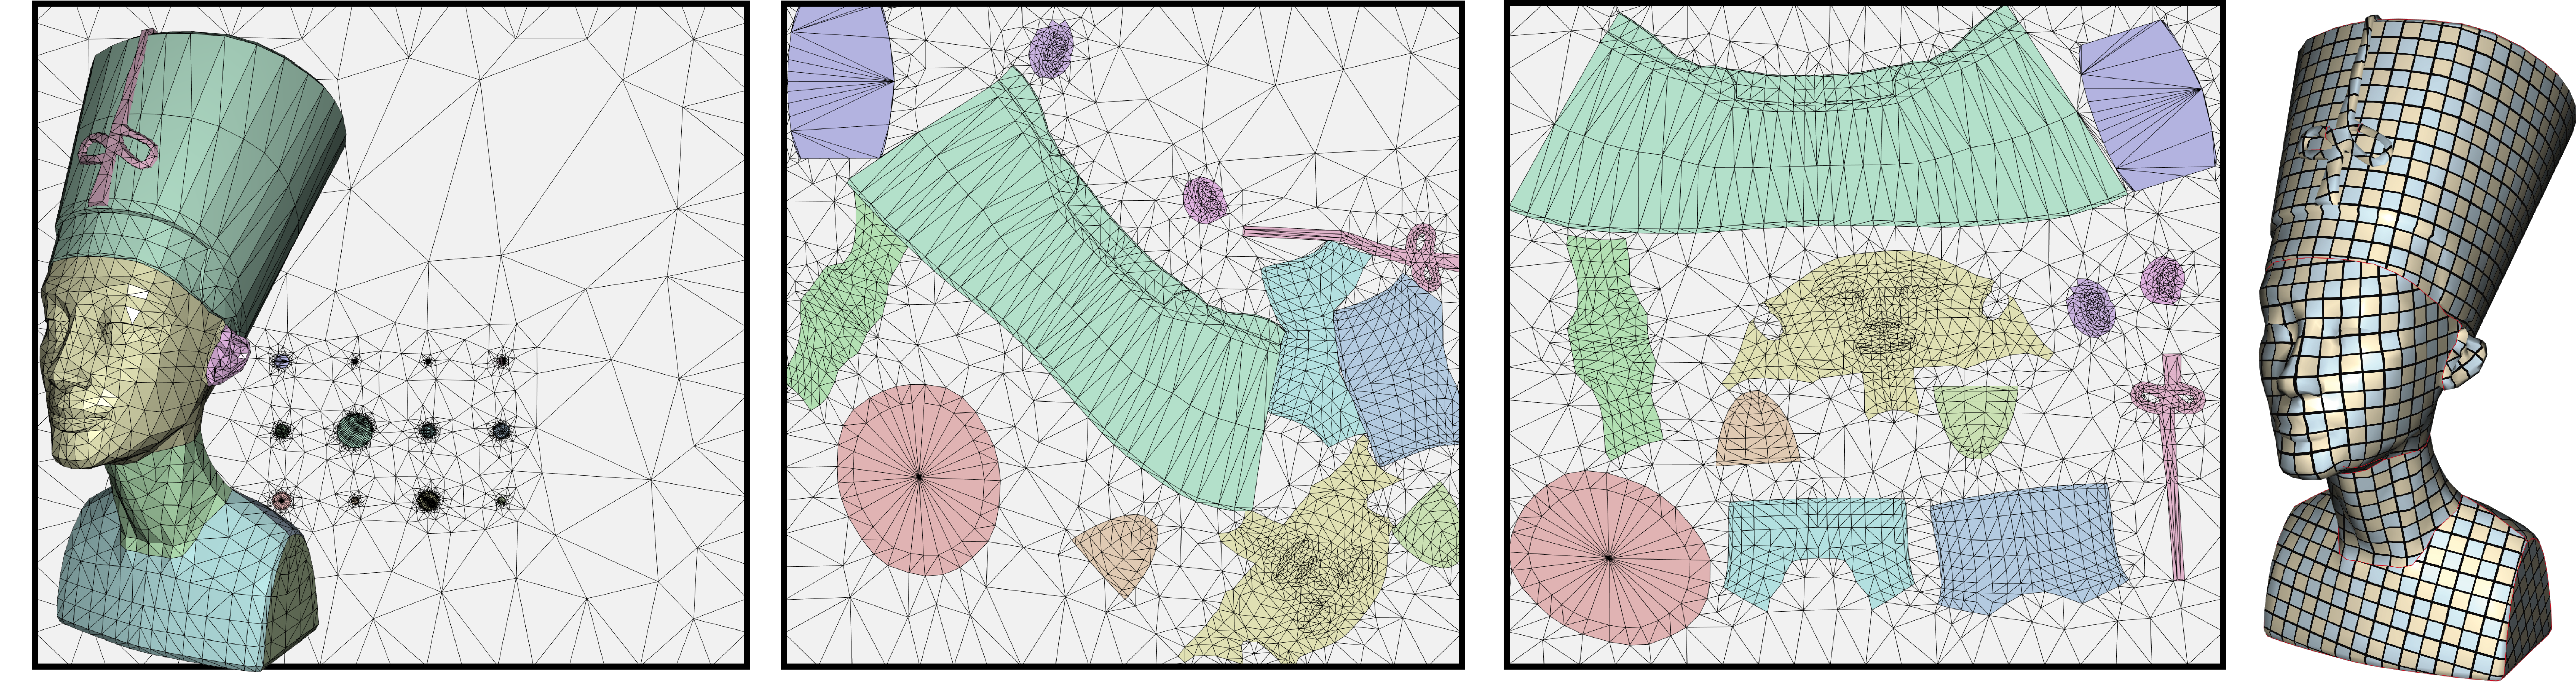
\includegraphics[width=\textwidth]{scaf-tex/figs/teaser}
 \caption{The Nefertiti model with prescribed seams is UV mapped by our algorithm. Each chart is bijective mapped into a circle or ring with Tutte's embedding and achieves minimal distortion in less than a second. The layout is further improved interactively and the final parametrized model is shown on the right. Our approach guarantees a valid UV map with no inverted elements or overlapping triangles. See the attaching video for the optimization and manual interaction.
}
 \label{scaf:fig:teaser}
\end{figure}

\section{Introduction}

The computation of discrete maps is a fundamental problem in computer graphics that has been extensively studied in the last three decades. The problem is challenging due to the large solution space
and the non-linearity of the desired properties ({in both} distortion measures and constraints). Algorithms for robustly and efficiently computing locally injective (i.e. non-flipping) maps have been only recently introduced \cite{Lipman:2012,Kovalsky:2016,rabinovich2017scalable} and are now having a major impact in many research areas outside of traditional texture mapping, including remeshing \cite{Bommes:2013}, image editing \cite{Poranne:2014}, and cultural heritage \cite{Pal:2014}.

In this chapter, we consider the problem of generating bijective maps, i.e. locally injective maps with {non-intersecting boundaries} %no self-overlapping triangles. 
This is a difficult problem, exacerbated by the fact that any pair of {boundary elements could overlap, leading to non-linear constraints whose number is quadratic in the size of the boundary}. %triangles could potentially overlap, leading to a quadratic number of non-linear constraints to satisfy {(yet, with locally injectivity, number of constraints can be seen as linear in terms of boundary elements \cite{Lipman:2013ArXiv}).} 
This problem is usually tackled by iteratively deforming an existing map, checking for overlaps after each step, and then preventing the overlap using constraints \cite{Harmon:2011} or penalty forces \cite{harmon2010robust}. These methods require a spatial acceleration structure to find the candidate pairs of overlapping elements and a resolution strategy that updates the map while avoiding the detected overlaps. {However, t}he newly computed displacement might {in turn} lead to new overlaps, and this process {has to be} performed iteratively {in the hope that} no  collisions are {left}. Difficult cases with many collisions might requires tens or hundreds of iterations before all the candidate intersecting pairs are detected.

Our approach sidesteps the need to find candidate self-intersections {based on a} simple observation: if the the entire ambient space {(with a fixed simple boundary)} is tessellated, then local injectivity implies global bijectivity \cite{Zhang:2005,Lipman:2013ArXiv,Muller:2015}. We {thus} propose an optimization framework based on this idea {making it possible to} leverage recent techniques for {locally} injective maps; our algorithm is simple to implement, robust, and two orders of magnitude faster than competing methods.

\paragraph{Overview.} Given an input bijective map represented by a discrete triangle mesh and its mapped vertex locations, we create a new scaffold mesh for a bounding box that contains the initial, mapped triangle mesh (Figure \ref{scaf:fig:teaser}) and conforms to its boundary. We then optimize for the desired property of the map (such as distortion, positional constraints, etc.) while ensuring that no triangle will flip. This property is achieved using a variational formulation that combines a user-defined energy for the map with a regularization term that allows the scaffold to freely deform without hindering the optimization of the map properties. During the optimization, we refine and optimize the connectivity of the scaffold mesh to prevent possible locking situations.

{While a scaffold mesh has been already used in previous works \cite{Zhang:2005,Misztal:2012,Muller:2015}, we propose to use an isometric distortion energy on the scaffold mesh, with the reference reset to the current rest pose at each iteration, and an online remeshing strategy. Our scaffold energy aims for "isometry to the current iteration", which resembles how plasticity is usually modeled in elasto-plastic simulations --- this leads to a global and natural deformation of the scaffold elements that opens up space for the evolving boundary and allows for an efficient optimization using recent numerical methods for locally injective maps \cite{rabinovich2017scalable}.}

We demonstrate the practical utility of our algorithm in the context of single patch mesh parametrization by producing distortion minimizing bijective maps for a collection of {119} challenging models. Our algorithm is ideal to compute tight UV maps for models with multiple connected components and seams as we demonstrate in our interactive texture packing experiments. Our algorithm can also be easily extended to 3D by replacing the triangular scaffold with one composed of tetrahedra. For the 3D case, we show that our method can be used to deform surfaces preventing self-intersections and to remove self-intersection from existing genus-0 surfaces when paired with a mean conformalized flow \cite{Kazhdan:2012,Sacht:2013}.

In the additional material, we provide a video (showing the optimization iterations) and the input/output meshes for each figure in the paper. To foster replicability of results, we will release an open-source reference implementation of our algorithm. 

\paragraph{Contribution.}
\begin{itemize}
\vspace{-1em}
\item We enhance the idea of scaffolding to the context of efficient geometric optimization with the "isometry to the current iteration" energy. This allows scaffold elements to freely open up space for the chart boundary to take larger steps than otherwise possible (Figure 12), as well as oblivious to the triangulation at each iteration.
\item To the best of our knowledge, ours is the first method that can bijectively parameterize large, complex models efficiently and robustly.
\item Our method provides an intuitive and simple way to prevent degenerate elements, which is required to avoid locking (different from \cite{Muller:2015}, where they must allow flip to exert force), and handles challenging cases such as those in Figure 5. 
Our formulation unifies geometric optimization problems in 2D/3D
%\item 
%Our work is also greatly motivated by practical considerations: we are not aware of any method that can robustly/efficiently compute bijective maps in 2D and 3D, which is fundamental and appears in many graphics and geometry processing tasks. We believe our proposal is a major step forward in solving this problem, simple to implement, and extremely robust.
\end{itemize}

\section{Method}

Our method, Simplicial Complex Augmentation Framework (SCAF) utilizes a scaffold structure to robustly compute a bijective map between a pair of simplicial meshes with the same connectivity. SCAF is specialized for the context of geometric optimization, i.e. we are interested in maps with low distortion and optionally satisfying a set of geometric constraints. We assume our maps are continuous and piecewise affine, i.e. the map deforms every simplex with an affine deformation. Thus, we can fully define the map using the image of its vertices.

% SCAFfolding Conforming Auxiliary Faces
 Our algorithm uses a discrete, bijective identity map (encoded as a non-overlapping and non-flipping triangle/tetrahedral mesh)  as initialization and then iteratively refines it, displacing the vertices while always ensuring that it remains bijective. Our method is composed of three stages: (1) augment the initial mesh with a scaffold, filling a bounding box around the initial map image; (2) optimize the extended mesh (scaffold included), reducing the geometric distortion of the map; (3) update the vertices and scaffold, enlarging the bounding box if necessary, to improve the quality of the triangulation. Steps (2) and (3) are iterated until the quality of the map is deemed sufficient.  

\subsection{General Formulation} \label{sec:general_form}
Denote the input simplicial mesh by $\Mesh = (\V,\F)$ with a single, simple boundary representing a compact $d$-dimensional manifold embedded in the $d$-dimensional Euclidean space, where $\V$ is the set of $n$-vertices and $\F$ is the set of $m$-simplices. Our goal is to compute a continuous and piecewise affine mapping 
$\Phi : \Mesh \rightarrow \R^{d}$ with $\Omega := \Phi(\Mesh) = (\V',\F)$ the resulting simplicial mesh with the same connectivity as $\Mesh$. 

We are interested in the bijective map that minimizes a given type of geometric energy:
\begin{align}
\begin{split}\label{eq:bijective_energy}
    \min_{\V'}& \quad E_{\Mesh} (\Phi) \\
    \text{s.t.}& \quad \Phi\text{ is bijective},
\end{split}
\end{align}
where $E_{\Mesh}$ is a user-defined geometric energy.

\paragraph{Reduction to Local Orientation Preservation.}  A sufficient %\revision{and necessary} 
condition for the simplicial map 
$\Phi: M\rightarrow \Omega $ to be bijective is that the map preserves orientation and its restriction to the boundary $\Phi|_{\partial M} : \partial M \rightarrow \partial \Omega$ is bijective~\cite{Lipman:2013ArXiv}. In this light, we are able to take advantage of the following simple construction (Figure \ref{scaf:fig:construction}): the algorithm extends the axis aligned bounding box of $M$ to get a $d$-orthotope and fills the enclosed region with a scaffold simplicial complex to form a simplicial complex mesh $D$ that includes and conforms to $M \subset D$. We can now define the continuous and piecewise affine map $\Psi : D \rightarrow D'$ with $\Phi = \Psi |_{M}$ where $\Psi|_{\partial D}$ is the identity map, and denote the scaffold region as $S = D\setminus M$. Now $\Phi$ is guaranteed to be bijective if $\Psi$ preserves orientation. Using this observation, we can translate the bijectivity into a local, orientation-preserving requirement defined per simplex.

\begin{figure}[h!]
\centering
    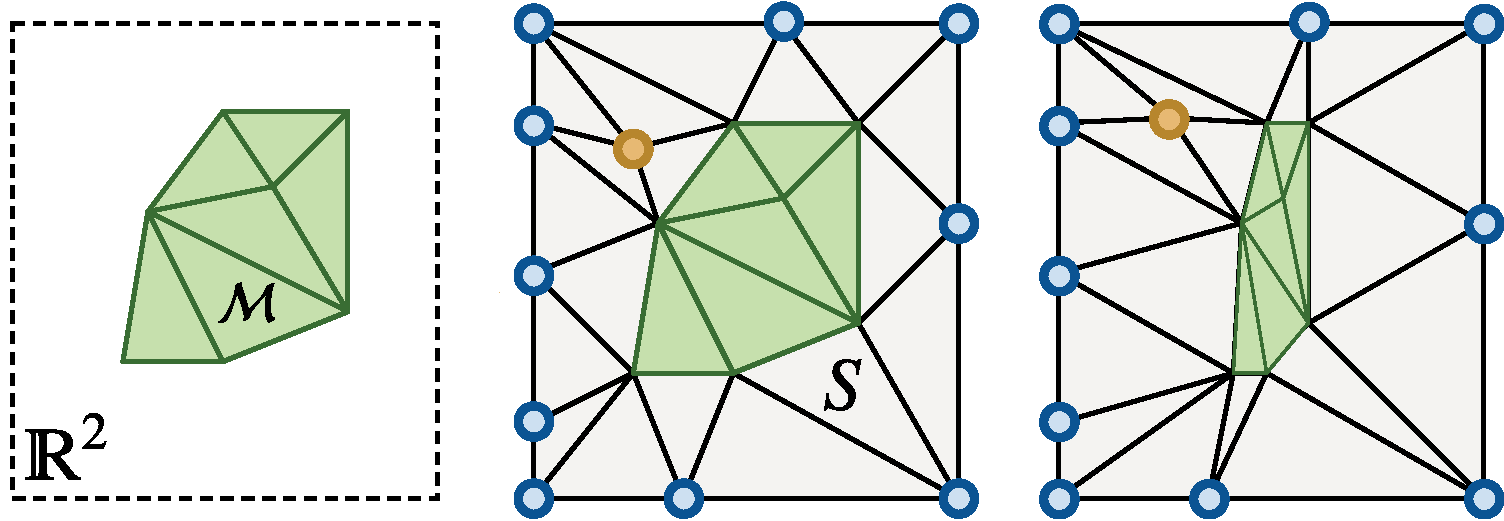
\includegraphics[width = \columnwidth]{scaf-tex/figs/scaffold_illustration}
\caption{The initial mesh $\Mesh$ (in green, left), is embedded in another mesh $D$ (in gray, middle) that covers a box in the ambient space and contains the same triangles as $\Mesh$. $D$ might contain additional points (orange). We denote the triangles that are in $D$ but not in $\Mesh$ as the scaffold $S$. Our algorithm deforms $D$, inducing a corresponding deformation on $\Mesh$ (right), while keeping the boundary (blue vertices) fixed and preventing changes in the triangle orientation.}
\label{scaf:fig:construction}
\end{figure}


 \paragraph{Variational Formulation} 
 Minimizing the distortion of $\Phi$ using the augmented map $\Psi$ poses an interesting challenge: what is the desired shape of the scaffold $S$? Ideally we would like the simplices in the scaffold to maintain their orientation and not affect the optimization in any other way. Such a requirement is difficult to model directly, since it is a discontinuous condition that is not well-suited for the variational framework that we would like to use to minimize $E_{\Mesh}$. 
 
 We propose a regularized version of this condition modeled with an energy $E_{\Mesh} (\Psi|_{S})$ that still diverges when elements change orientation and that mildly penalizes any non-rigid distortion.
 
 We choose a reweighted version of the symmetric Dirichlet energy $\Distort$~\cite{Smith:2015}, measured w.r.t. the Jacobian of the map $\Psi$ computed from the rest pose of $S$ for each simplex $f$,
\begin{equation}
    J_f := \nabla \Psi_f
\end{equation}
where $\Psi_f$ is the restriction of $\Psi$ over the simplex $f$, which is an affine map. We divide the energy of each scaffold simplex $f$ by its area $A_f$, and sum them up to obtain the final energy that favors an equal contribution regardless of the size of each scaffold simplex:
\begin{align}
    \begin{split}
    E_S(\Psi|_{S}) =&\sum_{f\in S} \frac{1}{A_f} \Distort(J_f) \\
    =&\sum_{f\in S} (\norm{J_f}_F^2 + \norm{J^{-1}_f}_F^2 -2d).
    \end{split}
\end{align}
The $-2d$ term ensures that the energy is 0 when $J_f = \mathbb{I}$. The map is then computed by summing the two terms:
\begin{align}
\begin{split}\label{eq:variational}
\min_{D} & \quad E_{\Mesh}(\Psi|_{\Mesh}) + \lambda E_{S} (\Psi|_{S}) \\
    \text{s.t.} & \quad \Psi|_{\partial D} \revision{\text{ is Identity}} \\ 
    & \quad \Psi \text{ preserves orientation}.
\end{split}
\end{align}
where $\lambda > 0$ is balancing the contribution of the two energies, decreasing as the optimization proceeds.

\paragraph{Iterative Regularization}
Solving this problem leads to a bijective and distortion minimizing map, but the regularizer will affect the stationary points of $E_{\Mesh}$, which is problematic, especially for large deformations.
%
To address this problem we iteratively minimize this energy, regenerating the scaffold at each iteration, and use the new scaffold as a rest pose for the regularization term $E_{S} (\Psi|_{S})$. This iterative procedure has two positive effects: (1) it acts as a proximal regularization term without inhibiting movement since the rest pose is updated at each iteration; (2) the meshing quality of the scaffold is high, which avoids locking configurations.

\paragraph{Interpolation Coefficient.}
We experimentally observed that our algorithm is robust to different choices of $\lambda$, generating indistinguishable results in most cases. However, $\lambda$ affects the convergence speed (Figure \ref{scaf:fig:different_weight}). We used $\lambda = \frac{1}{100}\frac{ E_{\Mesh}(\Psi|_{\Mesh})}{|S|}$ for all our experiments, where $|S|$ is the number of scaffold simplices.

\begin{figure}[h!]
\centering
    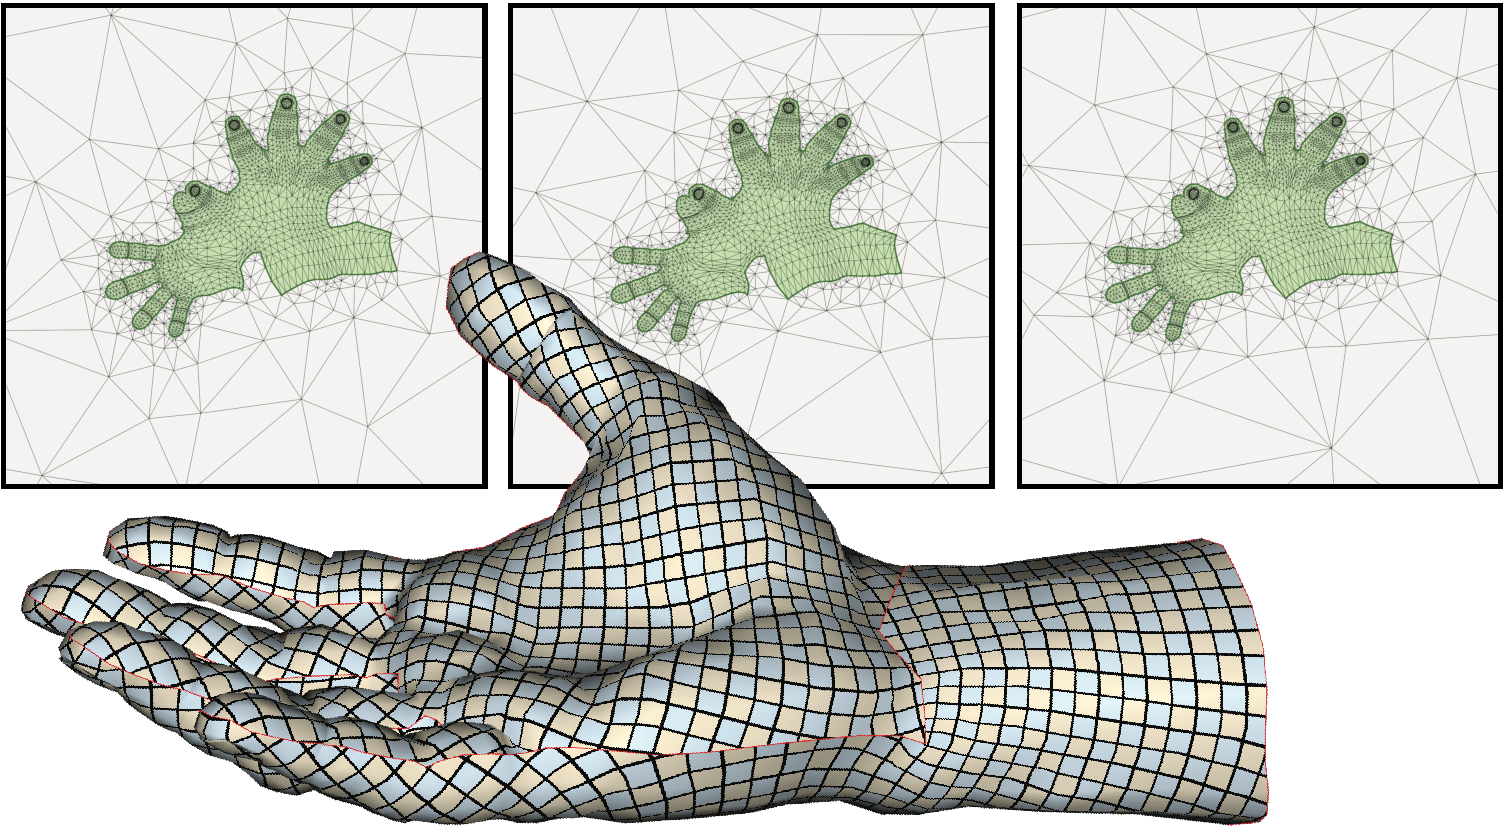
\includegraphics[width = \columnwidth]{scaf-tex/figs/hand_weight}
\caption{Different values of $\lambda$ do not affect the result, but they change the number of iterations needed. From left to right: we used a large weight (100x ours), our weight, and a small weight (0.01x ours). The optimization took 9,7, and 8 iterations, respectively, to reach the same energy level.}
\label{scaf:fig:different_weight}
\end{figure}

\paragraph{Solver.}
Since our energy is rotational invariant, we can minimize the energy with the same quadratic proxy proposed in SLIM \cite{Rabinovich:2017}, enriching the approach with the equality constraint needed to fix the boundary $\partial D$. We also employ the orientation-preserving line search \cite{Smith:2015} (with exact predicates \cite{Shewchuk:1996}) to ensure that no triangles can change orientation. Alternatively, other methods such as AQP \cite{Kovalsky:2016} could be used to minimize this energy. Since our approach changes the mesh connectivity at every iteration, AQP loses much of its advantages as the approximate \revision{H}essian must be recomputed at each iteration and not prefactored.  Therefore, our approach is an ideal fit for \cite{Rabinovich:2017}, which takes large steps at every iteration without relying on a constant, prefactored matrix at each iteration. For practical applications, SLIM iterations are sufficient to minimize the energy to acceptable levels. For two  stress tests (figures \ref{scaf:fig:recovering} and \ref{scaf:fig:smith}) we used the result of SLIM as a warm start for a Newton optimization (as suggested by \cite{Rabinovich:2017}), which quickly converges to a numerical minimum.

\subsection{Surface Parametrization}
Our framework can be used for many applications, one of which is computing a bijective surface parametrization from a 3D surface into the UV  plane. We follow \cite{Liu:2008} and assume that each 3D triangle $f^{3D}$ is equipped with a rigid transformation $R_f$ such that applying $R_f$ to $f^{3D}$ maps $f^{3D}$ to the plane. Given this transformed triangle $f$, we can now measure the distortion of the map using the Jacobian of the affine transformation (a $2\times2$ matrix) from $R_f(f^{3D})$ to $f$, the location of the triangle in the parametrization.

\paragraph{Initialization} Our method is initialized with Tutte's embedding algorithm~\cite{Tutte:1963}:
\[\Phi^0 : \Mesh^{3D} \rightarrow \Omega^0,\]
where $\Omega^0$ is a simplicial disk domain. Then we construct a larger rectangular domain $D^0 \supset \Omega^0$, where $\partial D^0$ is an axis-aligned rectangle, and use Triangle \cite{Shewchuk:1996} to triangulate the region in between.  We enforce a quality bound of $20^\circ$ to obtain a graded mesh that is coarse on the boundary and conforming the boundary of $\Omega^0$. This grading implicitly produces an approximate inverse distance  weighting of the scaffold space with respect to the error function, which enables a larger deformation per iteration. Then we define $\Psi: D^0 \rightarrow D \subset \mathbb{R}^{2}$ and restrict $\Psi |_{\partial D^0}$ to be the identity.
% \DP{Can we drop this?}We denote the vertex coordinates in $D^0$ by $U^0$, and augmented face set by $\matS$, i.e., $D^0 = (\matU^0, \matF\cup \matS)$.

\paragraph{Mesh Improvement}
At the end of each iteration, we improve the quality of the scaffold. The reason for maintaining a good mesh quality is two-fold. 
First, as observed in \cite{Zhang:2005, Muller:2015}, fixing the scaffold will potentially prevent movement. Secondly, the quality of the scaffold affects the condition of the linear system in SLIM \cite{Rabinovich:2017}: a higher  quality leads to larger and more efficient iterations.

We resort to Triangle \cite{Shewchuk:1996} to create the initial scaffold and to regenerate the scaffold mesh in the improvement step. Our experiments show that, in 2D, it is faster to generate the mesh from scratch at every iteration instead of trying to optimize the scaffold using local operations as suggested in \cite{Muller:2015}. Since our solver makes large steps in each iteration, the scaffold requires significant connectivity changes each iteration, which explains why regenerating the triangulation is faster than local operations. This is in stark contrast with physical simulation scenarios where each iteration represents a small time step and, thus, a minor change in the vertex positions.

We demonstrate the effectiveness of the remeshing strategy in Figure \ref{scaf:fig:recovering} where our method recovers from a large rotation --- note that the scaffold is updated during the iterations and always leaves space for the map to move freely.

\begin{figure}[h]
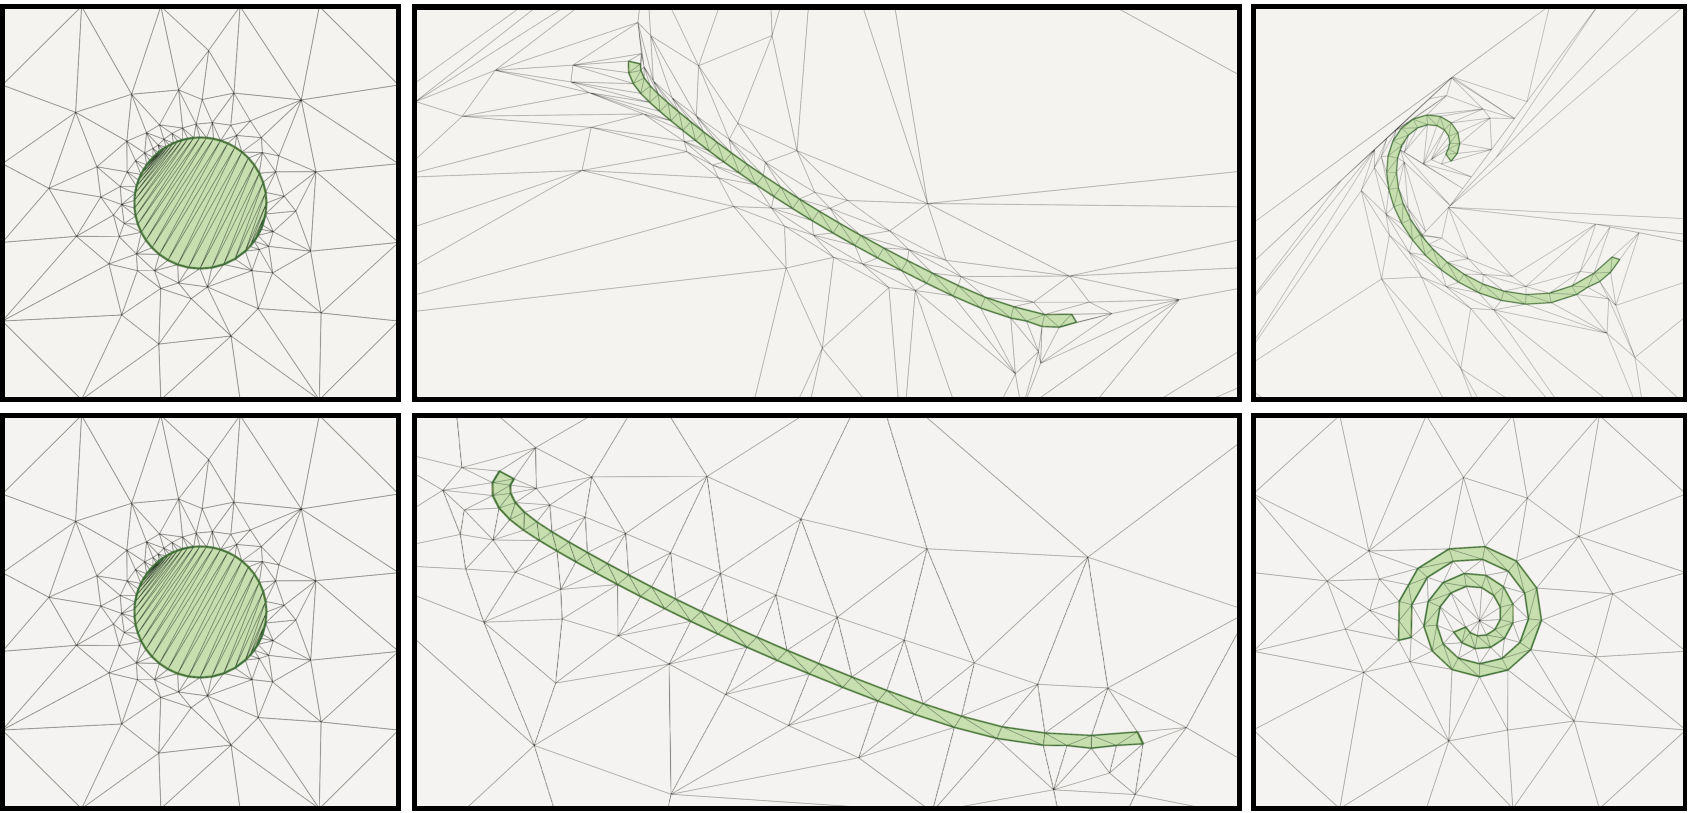
\includegraphics[width=\columnwidth]{scaf-tex/figs/coil-remeshing}
\caption{
\label{scaf:fig:recovering}
A bijective map from a circle (left) to a spiral (right) is computed without (top) and with (bottom) the iterative remeshing step. The slivers in the triangulation locks the optimization (top), preventing it from reaching the target shape.
% Recovering from a large rotation (up is remeshing: init, 30SLIM, 30 Newton; down is w/o reeshing 30 SLIM, 270 Newton) 
}
\end{figure}
\paragraph{Sliding \revision{\& Degeneracy Prevention}}
As the optimization proceeds and some of the boundary elements get closer, some of the scaffold triangles might (and often will) get smaller and smaller, restricting the amount of sliding that is allowed in one iteration as well as introducing numerical difficulties in computing the corresponding Jacobian $J_f$ \revision{whose singular values will approach infinity.}
% (Figure \ref{scaf:fig:slide}).  

To avoid this issue, we replace the degenerating target \revision{when computing its} Jacobian. For the triangles with an area smaller th\revision{an $\epsilon$, we use an equilateral triangle with area $\epsilon$ to compute the local Jacobian.} \revision{In our experiment,} we traverse through the boundary of the interior of the uv domain at the current iteration to find the minimum edge length $l$ \revision{and set} $\epsilon = \frac{l^2}{4}$.

A theoretical downside of this modification \revision{is that} it affects the distortion energy. We experimentally observed that the changes are negligible, and we thus used it for all our experiments. \revision{However, on the practical side}, it discourages fully degenerate elements --- this change, coupled with the orientation preserving line search \cite{Smith:2015}, makes our algorithm robust \revision{enough for the challenging stress tests shown in} Figure \ref{scaf:fig:miq_database}.
% \begin{figure}{h}
% 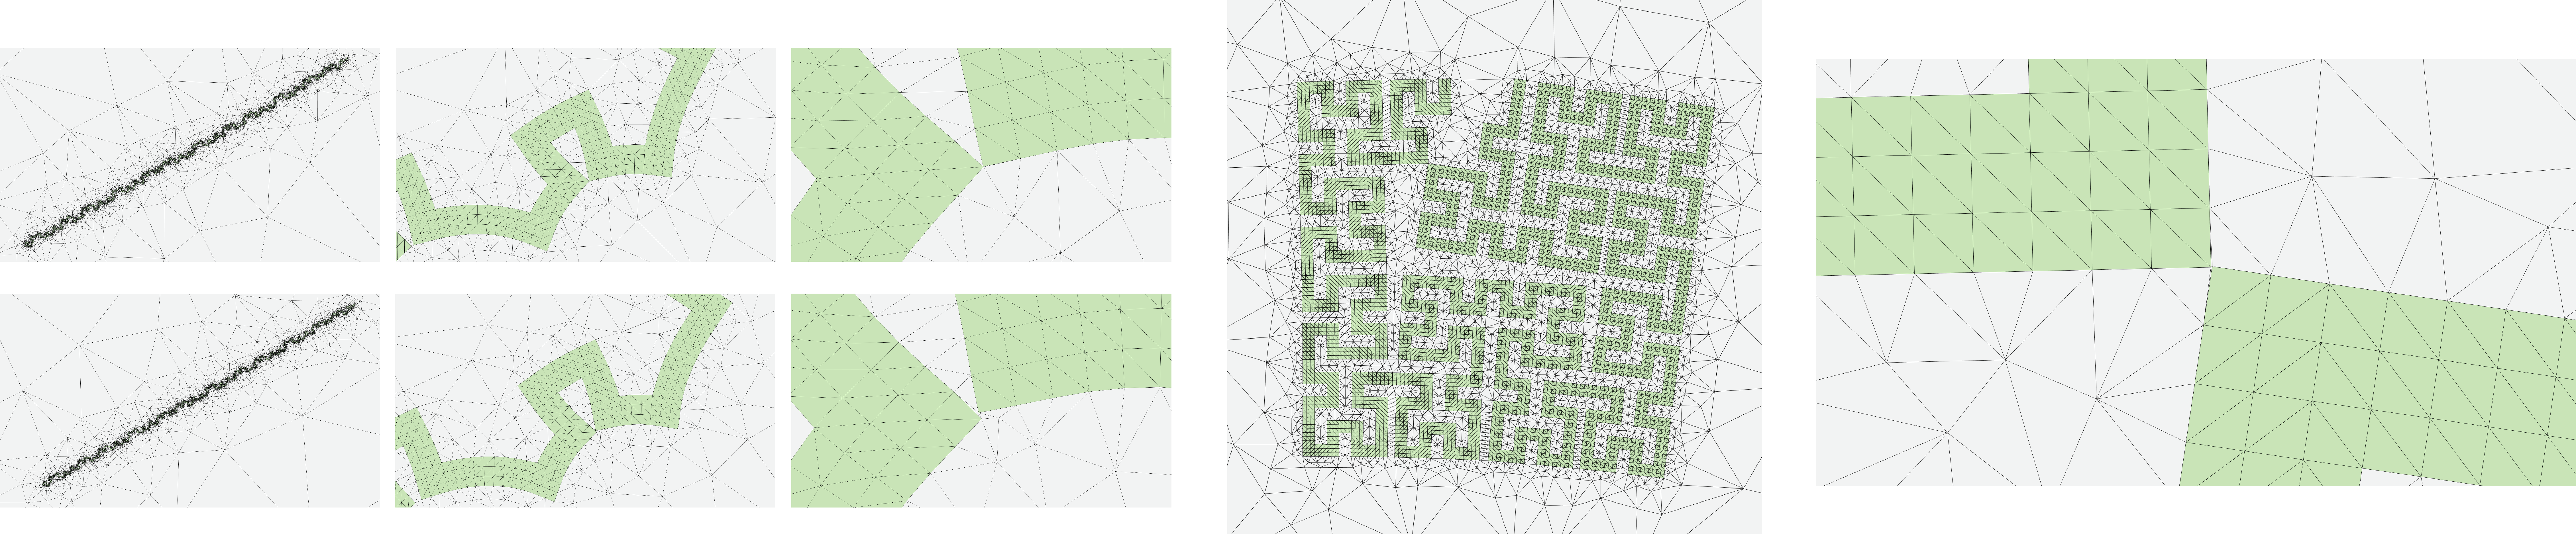
\includegraphics[width=8cm,height=4cm]{scaf-tex/figs/hilbert_area_threshold}
% \caption{
% Sliding example, one gets stuck the other one does not. \DP{TODO}}
% \label{scaf:fig:slide}
% \end{figure}

\subsection{Extension to 3D}

\revision{Our formulation naturally unifies bijective geometric optimization problems in 2D and 3D, so the} algorithm readily extends to the 3D case with only one major difference: the scaffold becomes a tetrahedral mesh, which is computationally more challenging to create and update.
\paragraph{\revision{Mesh Improvement}}
We use TetGen \cite{Si:2015} to generate the initial scaffold and the local operations proposed in \cite{Klingner:2009} to optimize the scaffold's quality in the subsequent iterations. 
%We describe our mesh improvement algorithm in details in Appendix \ref{appendix:improvement} \DP{TODO}.
%
It is unfortunately not possible to directly use TetGen at every iteration as we did with Triangle in the 2D case, since TetGen fails when boundaries get too close, which is common in our experiments.

\revision{
\paragraph{Guarantee} Similarly to the 2D case, we are guaranteed that no flipping or self-intersecting tetrahedra will occur since we are following an interior point strategy. Notice the contrast with Air Mesh \cite{Muller:2015} where only if penetration happens can the constraints be of effect. However, as pointed out in \cite{Dougherty2004}, the local operations we are performing may not be sufficient to explore the entire space of possible tetrahedralizations. %effective enough to explore the whole space of tessellation. 
Therefore, we cannot guarantee that the algorithm achieves the globally optimal solution.
}
\section{Results}
We implemented our algorithm in C++ using Eigen for linear algebra routines. We \revise{ran} our experiments on a desktop with a 4-core Intel i7  processor clocked at 4 GHz and 32 GB of memory \revise{but using only one thread on a single core}. For all experiments, the scaffold bounding box is computed by uniformly scaling by three times the bounding box of the image of the current map. 

\begin{figure}[t]
\includegraphics[width=8cm]{figs/database_demo}
\caption{Two models are cut using \cite{Bommes:2009} and bijectively parametrized using our algorithm. See the additional material for more examples.}
\label{scaf:fig:miq_database}
\vspace{-0.2cm}
\end{figure}

\paragraph{Robustness.} To demonstrate the robustness of our algorithm, we computed  bijective maps for all the 102 meshes parametrized by the MIQ algorithm \cite{Bommes:2009} \revise{and for the 17 meshes parametrized by  \cite{Myles:2014}} in the dataset proposed by \cite{Myles:2014}. The cuts in these meshes have been designed for locally injective parametrization that usually have major self-overlap. We use them as a stress test for the effectiveness and robustness of our method:  the cuts introduce a massive distortion in the Tutte initialization and lead to boundaries that are prone to overlap in hundreds of locations. Our method successfully creates bijective parametrizations for all these models with default parameters. We attach all the parametrized models in the additional material and show two examples in Figure \ref{scaf:fig:miq_database}. 


% To demonstrate robustness in 3D, we deform \DP{XX} surfaces simultaneosly, by prescribing positional constraints that are  We simulate the deformation of a material made of hundreds of elastic layers. We run the simulation both on a 2D slice and on the full 3D model in Figure \ref{scaf:fig:stresstestlayers}. For this example, we compare the result obtained with the SLIM solver proposed in this paper and with the AQP algorithm \cite{}. \DP{TODO after we will know how it looks.}

% \begin{figure}[h]
% 
\includegraphics[width=8cm]{figs/placeholder.png}
% \caption{Mille-feiulle, both in 2D and 3D \DP{TODO}}
% \label{scaf:fig:stresstestlayers}
% \end{figure}

\paragraph{Scalability.} Our methods scales gracefully to large datasets, similarly to \cite{Rabinovich:2017}. We repeat their scalability experiment, but producing bijective maps instead of just locally injective maps (Figure \ref{scaf:fig:scalability}). The behaviour is remarkably similar --- the density of the model (and consequently of the scaffold) does not affect the number of required iterations. 

\begin{figure}[t]
\includegraphics[width=\columnwidth]{figs/lucy-scalability}
\caption{We compare the distortion energy with respect to the number of iterations on a set of Lucy's meshes with different resolutions (from 1 to 12 million faces). In the center of the plot, we show the 1M Lucy model parametrized by our algorithm.
}
\label{scaf:fig:scalability}
\end{figure}

\paragraph{Texture Atlas Generation} 

UV mapping is a time consuming procedure required in most geometric modeling pipelines. Existing commercial tools provide the ability to flatten single patches and arrange them in UV layouts where multiple patches are tightly packed inside a rectangular domain, which is then loaded in the texture memory of a GPU. 

Our algorithm can bijectively parameterize a single patch (Figure \ref{scaf:fig:manuallycut}), avoiding the typical manual UV postprocessing required with traditional tools.  Our algorithm can also be used to create automatic UV charts of models with multiple connected components (or predefined cut edges). We show an example in Figure \ref{scaf:fig:packing2D} where we detected the connected components, bijectively map the patches into a set of circles (using a grid layout), and reduce their distortion using our algorithm. The result is a tight and automatic packing without resorting to any user-interaction. Additional interactive tools can further improve the atlas by dragging\&dropping regions or translating islands while ensuring that no overlaps are introduced (Figure \ref{scaf:fig:teaser}). We show interactive sessions using our packing tool in the additional material.

\begin{figure}[t]
\includegraphics[width=8cm]{figs/the_animal}
\caption{A mesh is cut by an artist into a single chart and parametrized using SLIM \protect\cite{Rabinovich:2017} (left) and with our algorithm (right). Note that local-injectivity is not sufficient for this model, since the global overlaps in the highlighted region prevent this parametrization from being a UV texture map. Our result (right) is guaranteed to be bijective.}
\label{scaf:fig:manuallycut}
\vspace{-0.2cm}
\end{figure}

\begin{figure}[t]
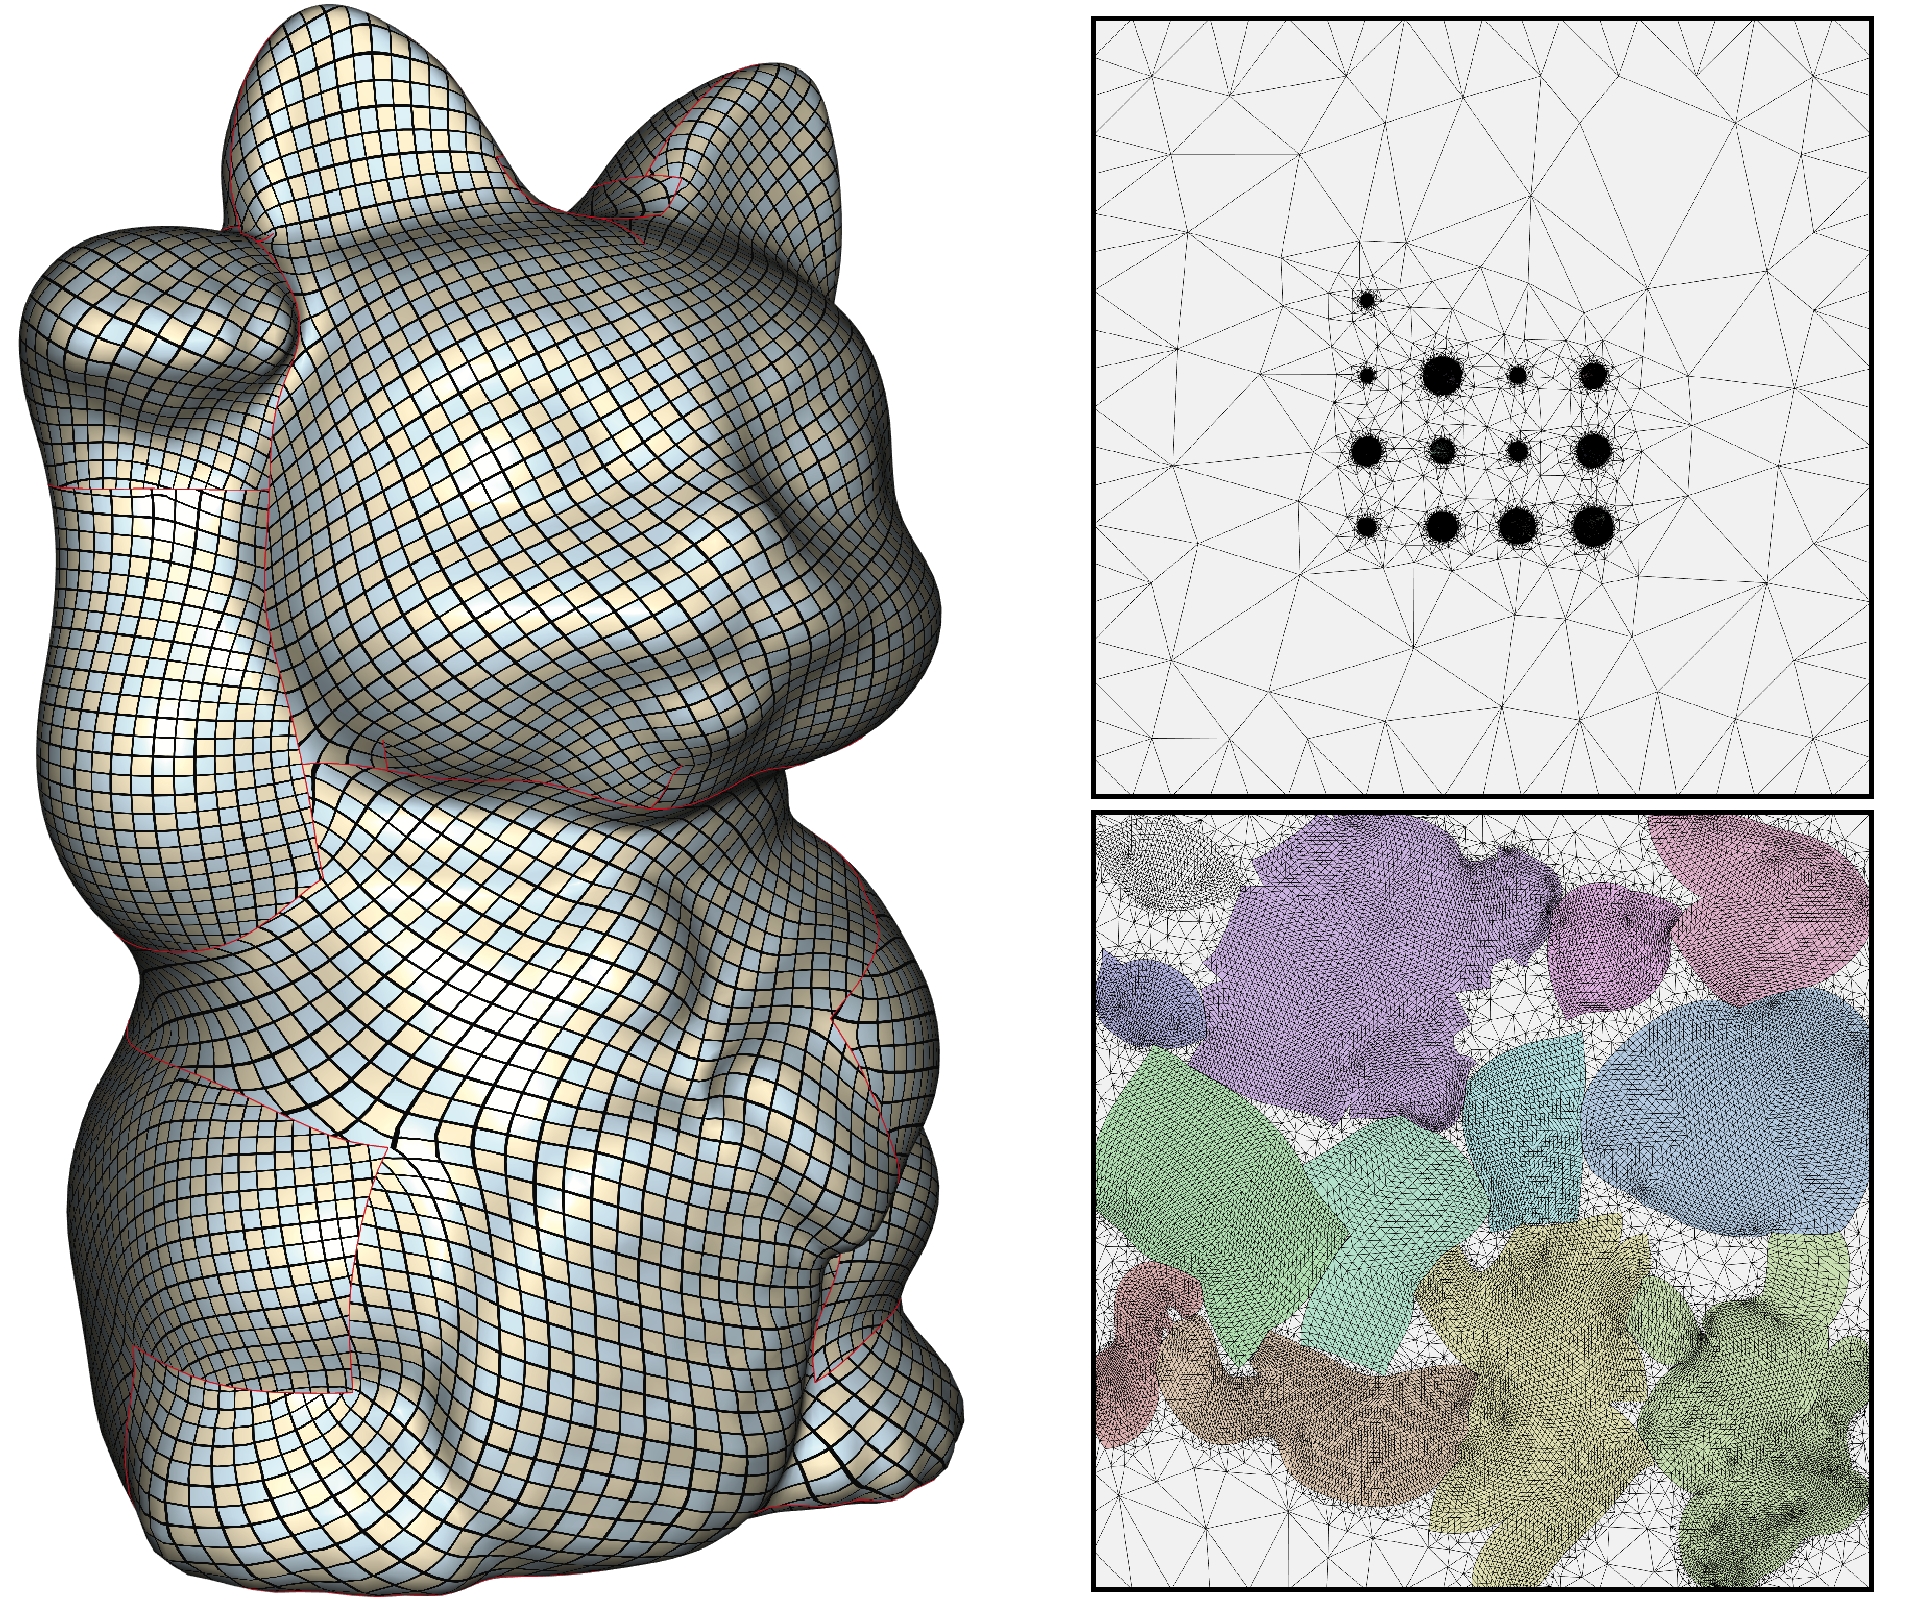
\includegraphics[width=\columnwidth]{figs/maneki_neko_colorful}
\caption{A model with multiple chart (left) is automatically parametrized in a texture atlas (bottom-right) by first mapping each component to a circle (top-right) and then minimizing the distortion.}
\label{scaf:fig:packing2D}
\end{figure}

\paragraph{Preventing Self-Intersections}
Our algorithm can be generalized to handle mixed dimension problems, such as the deformation of 2D surface in 3D space, while preventing self-intersections. In Figure \ref{scaf:fig:flow}, we demonstrate the use of our method to resolve self-intersections of surfaces. First we perform a conformalized flow \cite{Kazhdan:2012} using the algorithm proposed in \cite{Sacht:2013} to resolve any self-intersections.  While \cite{Sacht:2013} will resolve the intersections, the resulting surface may be geometrically far from the initial shape (see Figure \ref{scaf:fig:flow}).  Next we tetrahedralize the ambient space while conforming to the deformed surface mesh and minimize Equation \ref{eq:variational} with an additional energy term that strives to restore the rest pose geometry of the surface, using the surface ARAP energy proposed in \cite{Sorkine:2007}. The result is a surface similar to the original mesh, but without self-intersections. In this example, it is possible to observe that even dramatic changes of scale (on the foot) can be robustly handled by our parametrization algorithm.

A more challenging stress test is shown in Figure \ref{scaf:fig:rabbit}, where the bunny model is scaled up inside a box, to 30 times its original size. No self-intersections are introduced, despite the extreme, constrained deformation.

\begin{figure}[t]
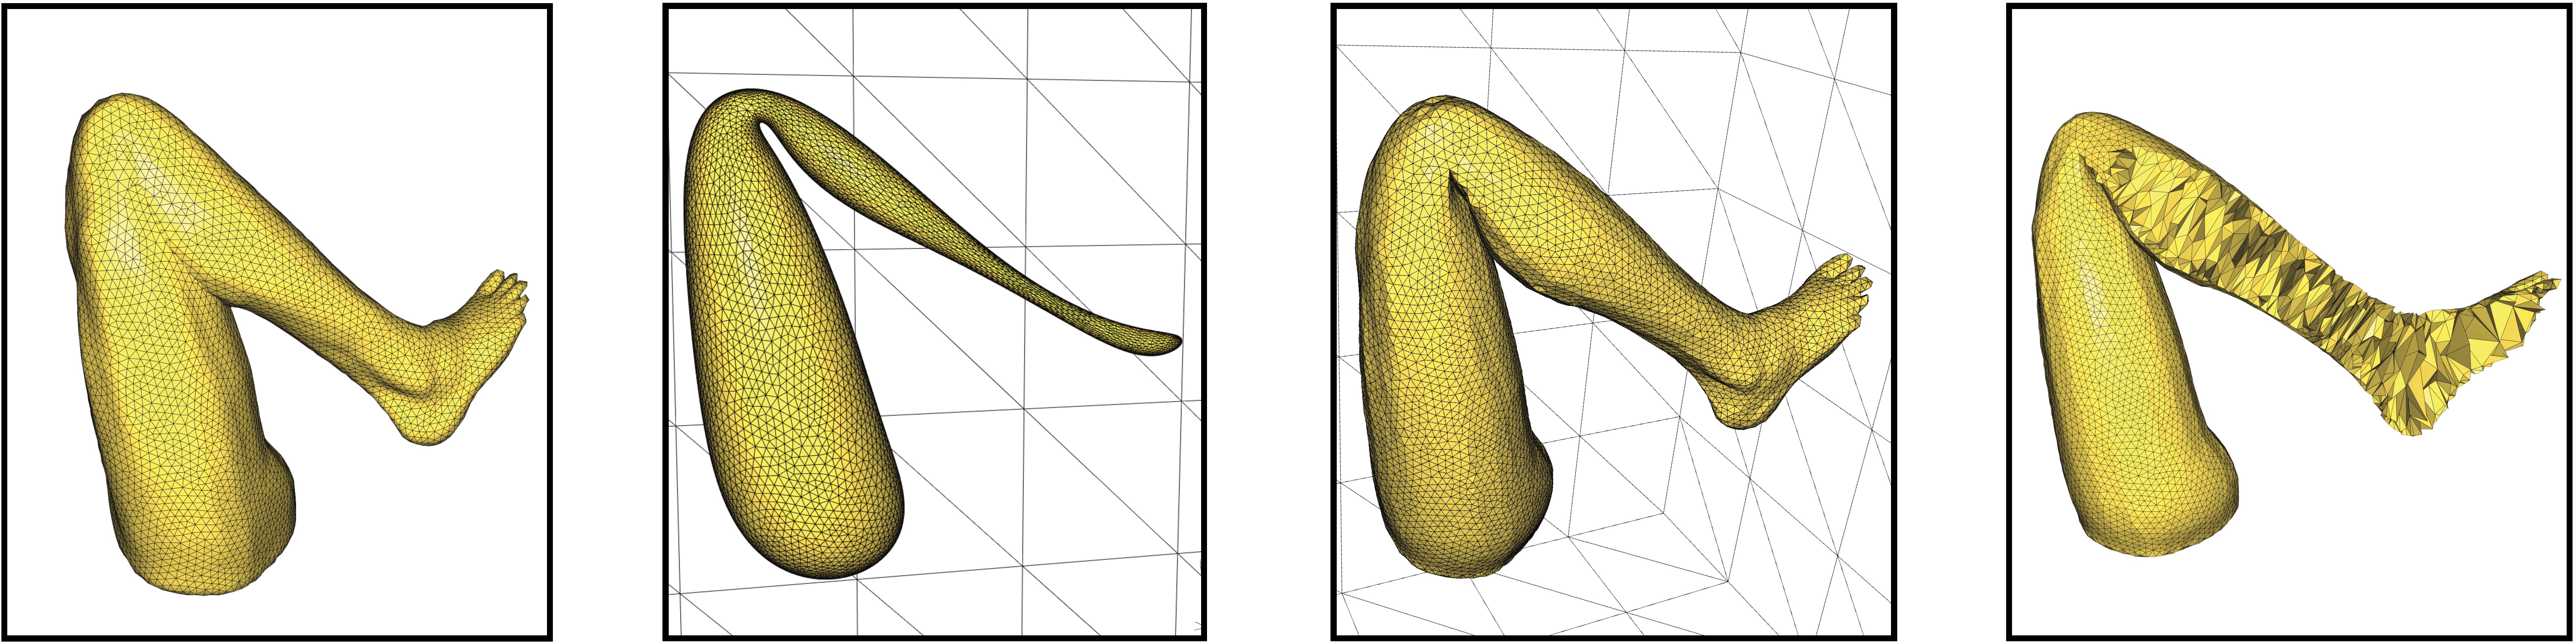
\includegraphics[width=\columnwidth]{figs/leg-flow}
\caption{We remove the self-intersections from a genus 0 model using the conformalized flow \protect\cite{Kazhdan:2012,Sacht:2013}. The flow is inverted, while using our algorithm to compute a bijective volumetric map, to recover a self-intersection free version of the original surface. The final model can now be meshed using TetGen, since it is free from self-intersections.}
\vspace{-0.2cm}
\label{scaf:fig:flow}
\end{figure}

\begin{figure}[t]
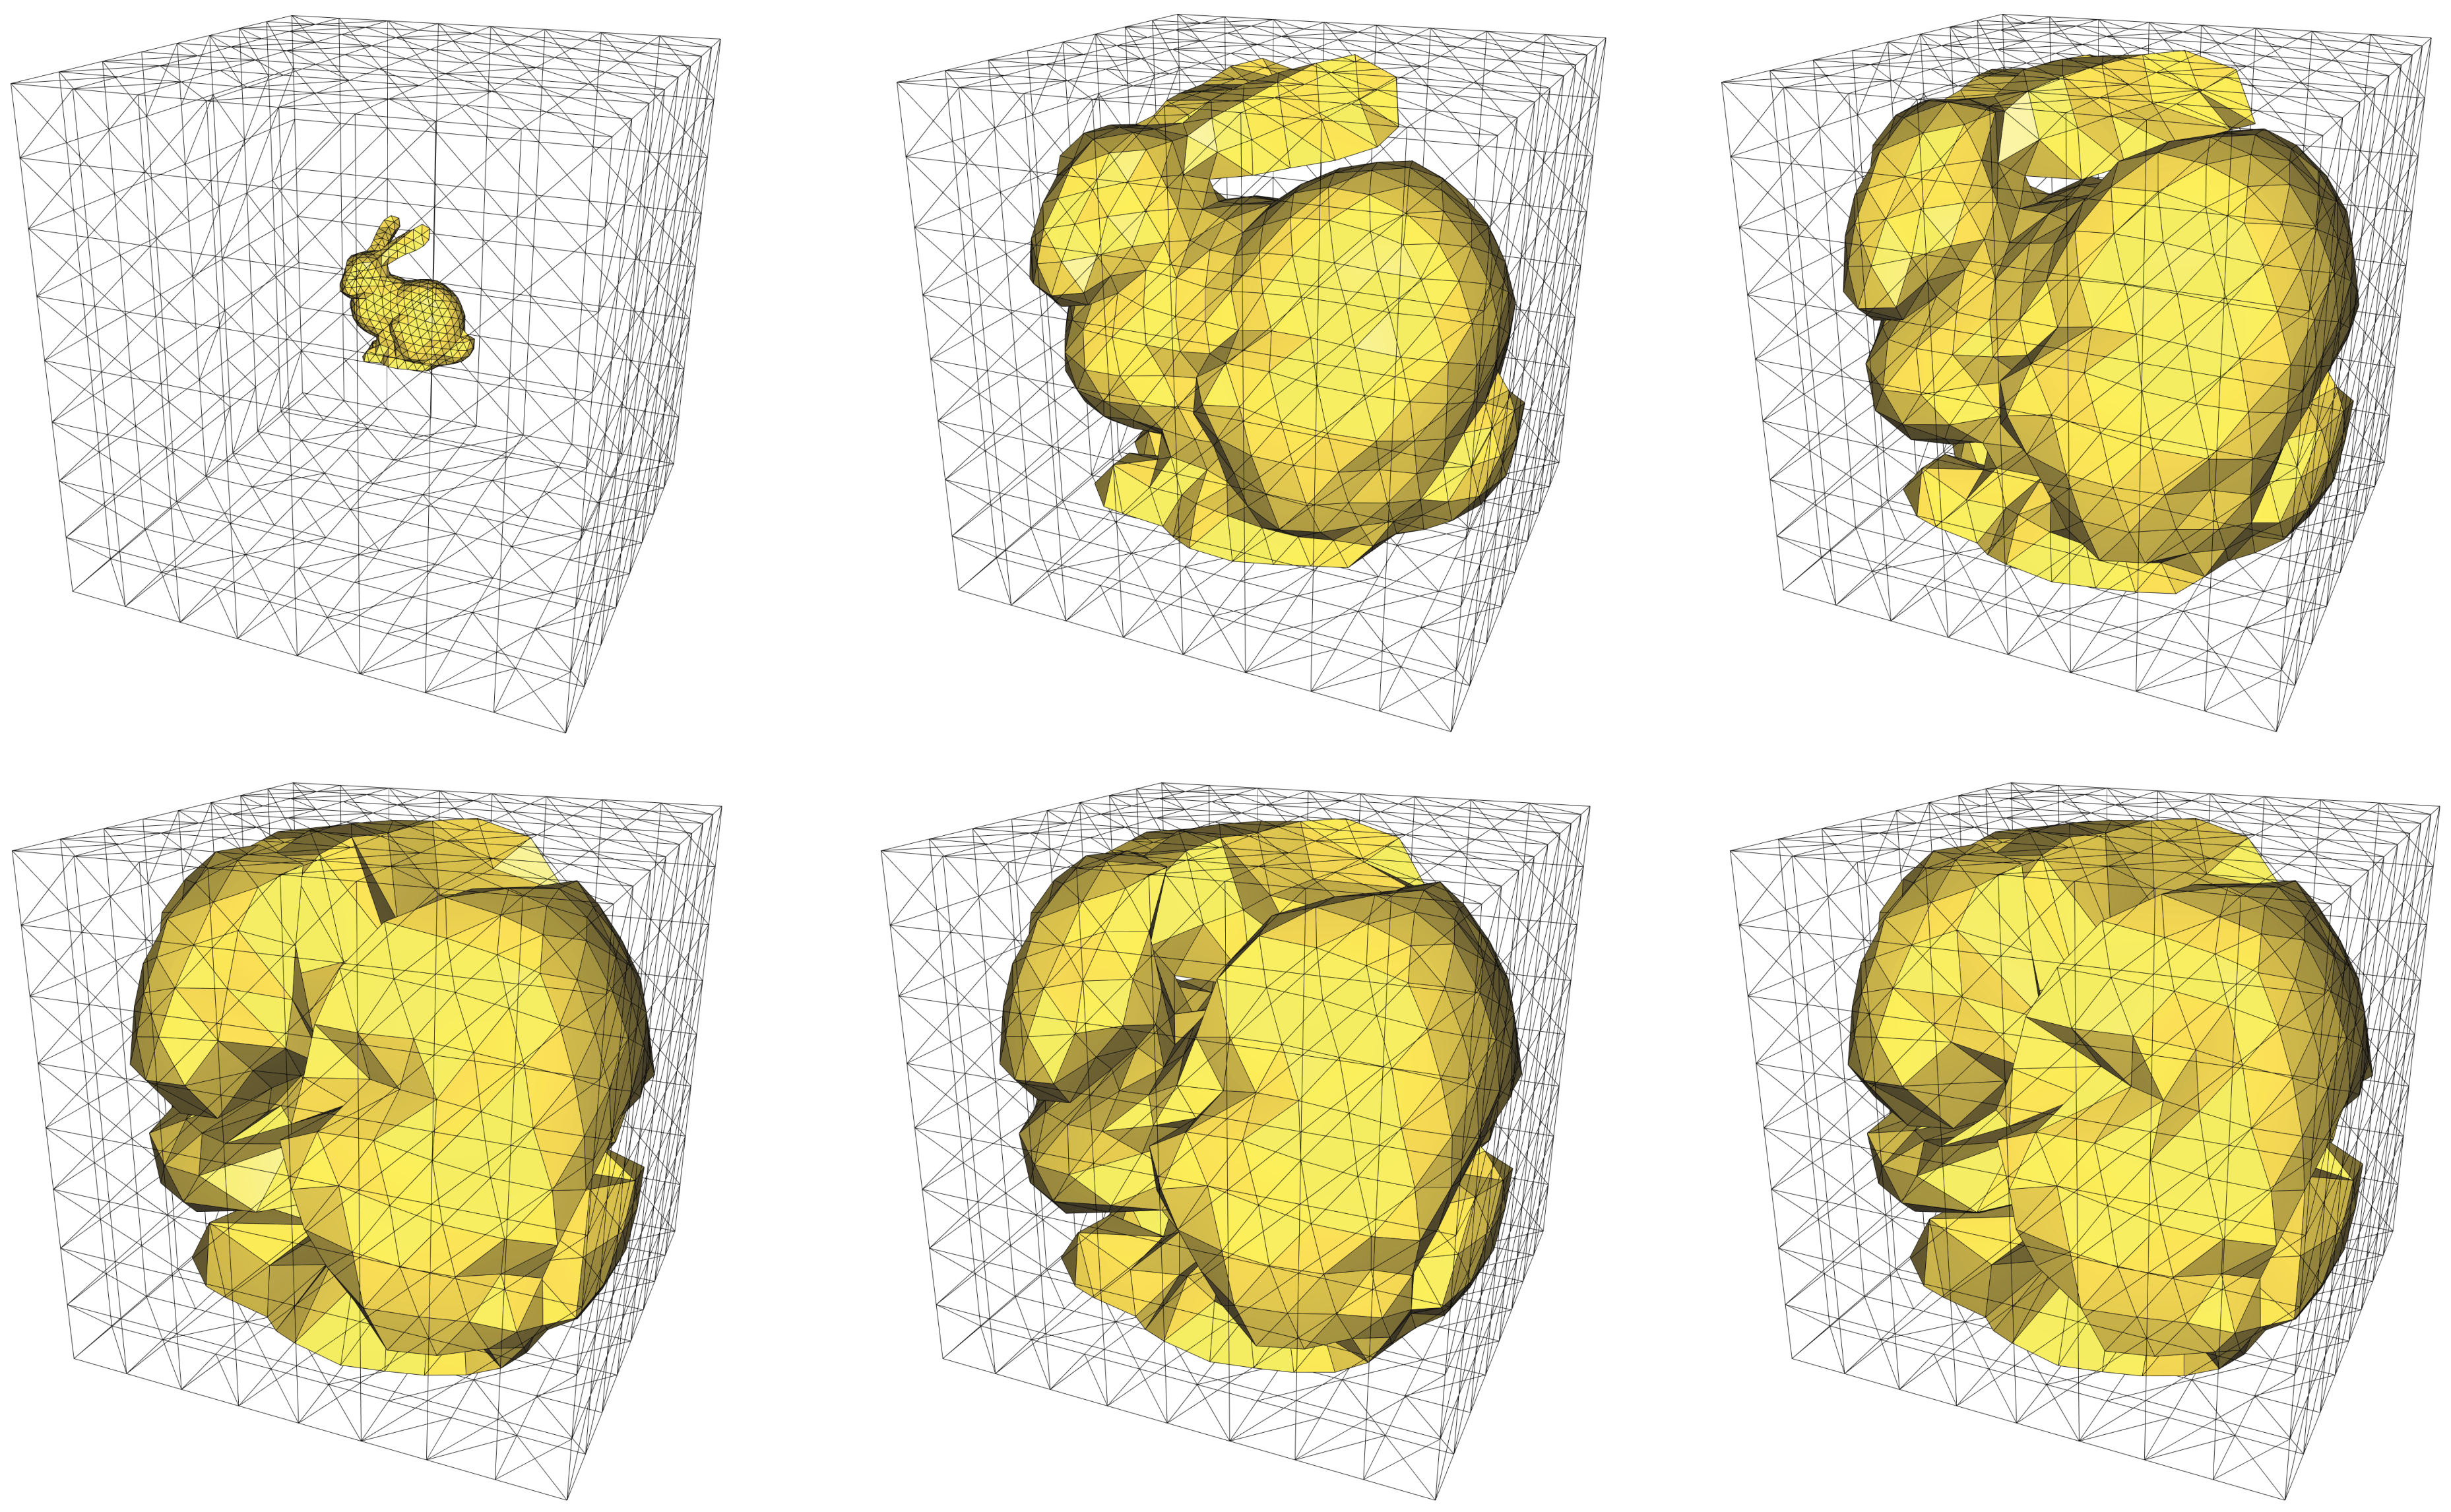
\includegraphics[width=0.8\columnwidth]{figs/rabbit_grow}
\caption{We grow a bunny inside a box, while preventing  self-intersections. We show the result after 0,10,20,30,40, and 50 iterations.}
\label{scaf:fig:rabbit}
\end{figure}


\paragraph{Comparison with \cite{Smith:2015}}
The algorithm closest to ours is \cite{Smith:2015}, which tackles a similar problem (restricted to the 2D case). We replicated the space filling curve experiment and obtained remarkably similar results, where our running time is 96s, compared with 8,472s for \cite{Smith:2015} (88 times faster). We show in Figure \ref{scaf:fig:smith} a more challenging experiment with a subdivided version of the space filling curve to emphasize the performance difference: our algorithm converges in 39 minutes, while \cite{Smith:2015} did not converge after 5 days and 21 hours. For this example, we used the procedure suggested in \cite{Rabinovich:2017}: we performed a few iterations minimizing the quadratic proxy and then switch to a traditional newton method until numerical convergence. A video of the optimization is provided in the additional material.

\begin{figure}[t]
\includegraphics[width=\columnwidth]{figs/dense_hilbert}
\caption{\revise{We repeat the challenging test in \cite{Smith:2015} with a subdivided version of their Hilbert curve to increase the triangle count. Our method starts from a disc (upper left), gracefully extends (upper right), and reaches the same minimum (lower left) in 39 minutes whereas \cite{Smith:2015} didn't terminate more than 5 days (lower right), highlighting our performance boost of over 200 times.
}}
\label{scaf:fig:smith}
\vspace{-0.2cm}
\end{figure}

\begin{figure}[t]
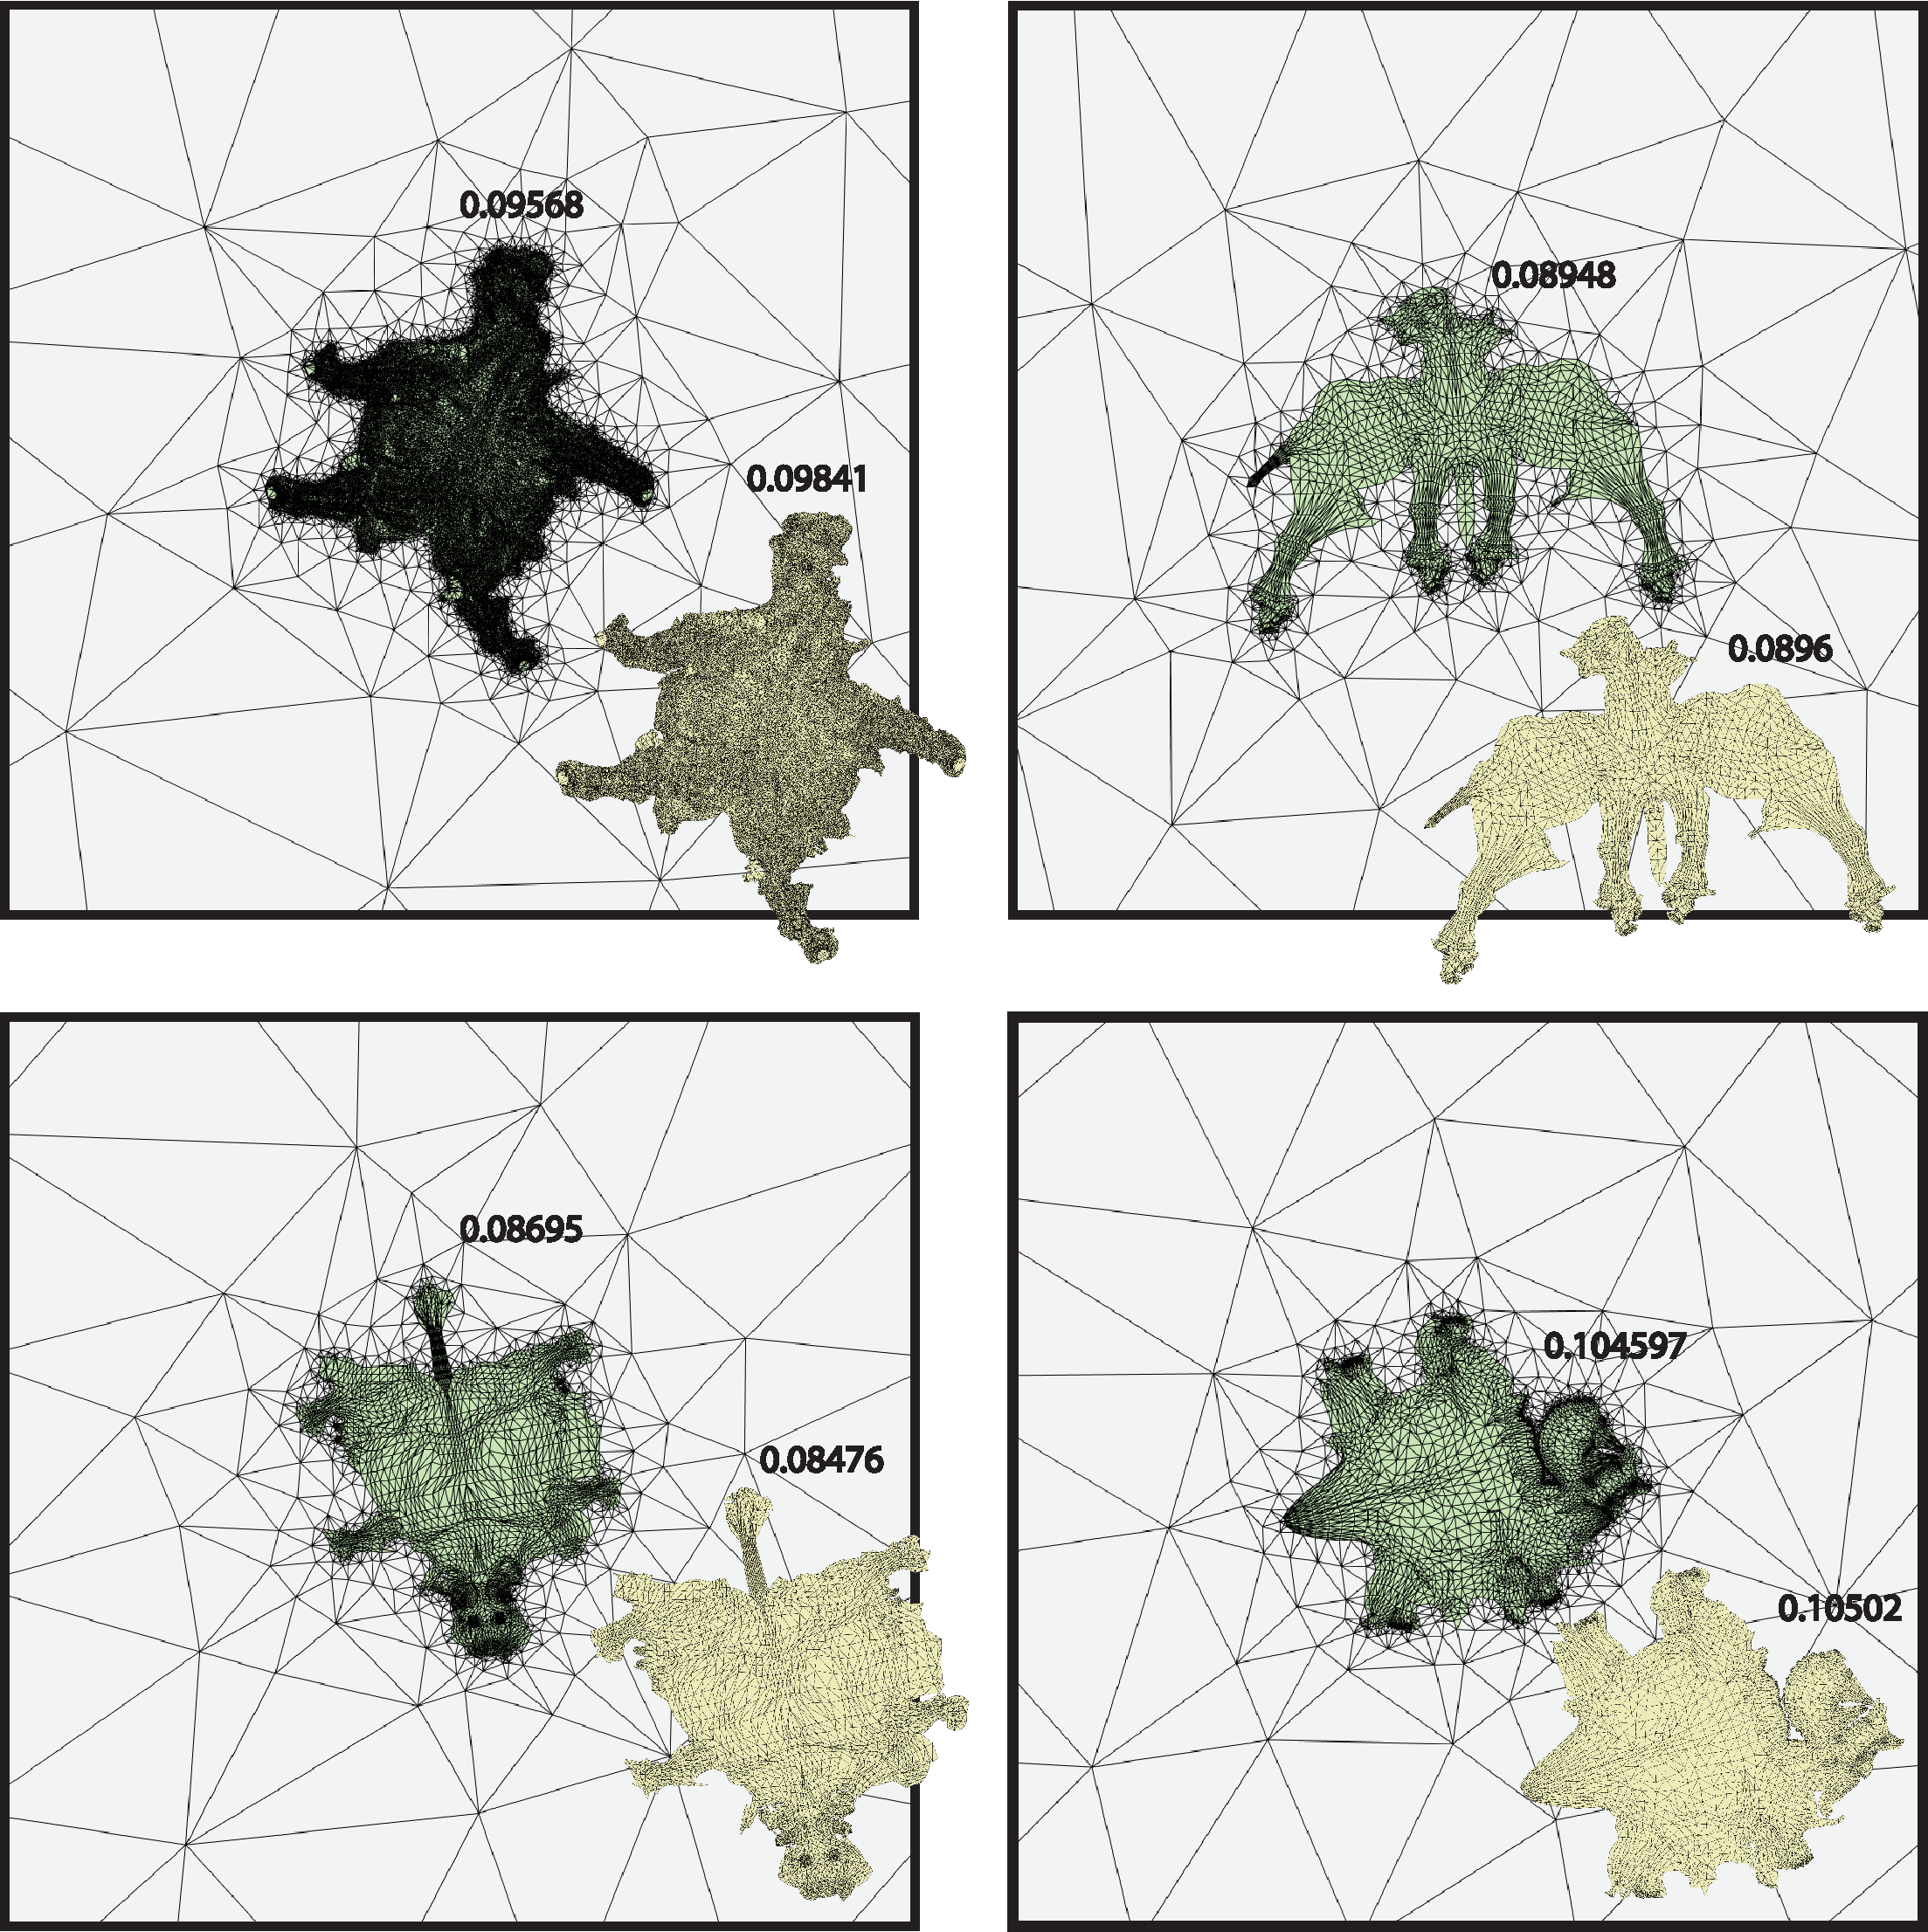
\includegraphics[width=\columnwidth]{figs/compare_smith}
\caption{\revise{We apply our algorithm on 4 models used in \cite{Smith:2015} (using the same stopping criteria) obtaining visually identical results. Distortion errors produced by our algorithm (outer) and theirs (inner) are shown in black.
}}
\label{scaf:fig:smith-all}
\vspace{-0.2cm}
\end{figure}

\revise{Our method produces results that are visually identical to \cite{Smith:2015}. In Figure  \ref{scaf:fig:smith-all} we repeat the experiments shown in \cite{Smith:2015}, stopping our optimization at the same energy value.}

\paragraph{Local vs Global Optimization} 

Both \cite{Zhang:2005} and \cite{Misztal:2012} use a construction similar to ours to generate bijective maps (Section \ref{sec:related}). Both methods explicitly prevent changes of orientation using a local approach: they optimize the map using coordinate descent iterations \cite{SolomonBook} allowing only one vertex at a time to move in its 1-ring and thus ensuring that no triangle flip. This strategy severely limits the maximal displacement per iteration and restricts the step to the size of the 1-rings. Such a restriction makes these methods impractical for parametrization applications since the difference in scale between the Tutte's embedding and the final result is extreme (the ratio of min and max triangle area is $10^{-6}$ in Figure \ref{scaf:fig:largestep}). We show an example of one of our iterations in Figure \ref{scaf:fig:largestep}, where the highlighted vertex traversed a distance of ~150 times the size of the average edge length of its 1-ring in one single step. Using coordinate descent would have required hundreds of iterations to achieve the same effect. 

\begin{figure}[t]
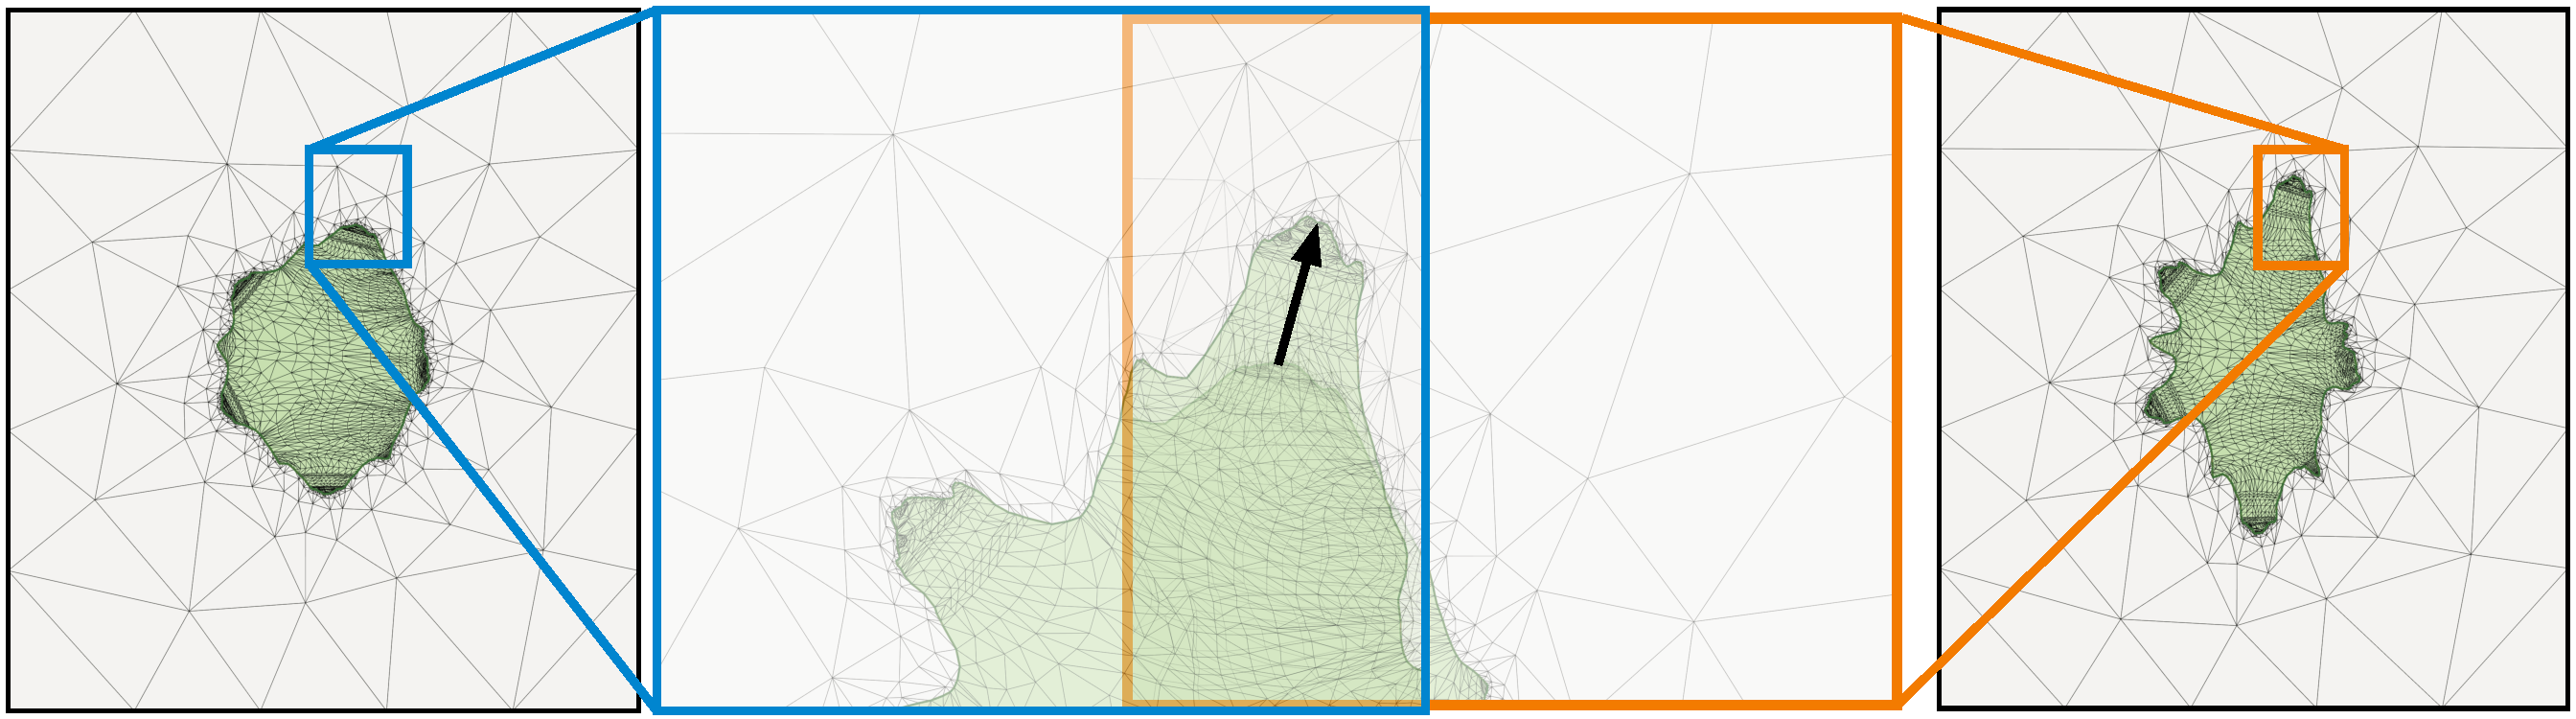
\includegraphics[width=\columnwidth]{figs/camel_step.pdf}
\caption{A single iteration of our algorithm (from left to right) drastically reduces the distortion. The black vector in the center is ~150 times longer than the average edge length of its 1-ring. Iterative methods would need thousands of iterations to achieve a similar progress.}
\vspace{-0.3cm}
\label{scaf:fig:largestep}
\end{figure}

\revise{
% what about... the original is convoluting the metric on the scaffold with the independence to orientation
Despite the orientation-dependent box used as scaffold boundary, our optimization produces results that are, in practice, independent of orientation.  We show this effect in Figure~\ref{scaf:fig:random-rotate} where we initialize the optimization with 1000 randomly rotated Tutte's mappings of the same camel model and run our optimization.  The isometric distortion of the model after 50 iterations is quite similar in all trials (the minimum, maximum, average, standard deviation of distortion errors in all 1000 runs are 0.1086, 0.1107, 0.1095, 3.2698e-4 resp.) indicating very little change based on the initial orientation.
%Since we enforce an isometric energy to the scaffold, translation and rotation is encouraged to make space for the evolving interior boundary. We are able to observe this effect by performing the experiment in Fig. \ref{scaf:fig:random-rotate}. Our algorithm is initialized with 1000 randomly rotated Tutte's mappings of the same camel model, then the isometric distortion of the model after 50 iterations is similar enough (the minimum, maximum, average, standard deviation of distortion errors in all 1000 runs are 0.1086, 0.1107, 0.1095, 3.2698e-4 resp.), indicating very little change based on the initial orientation.
}
\begin{figure}[t]
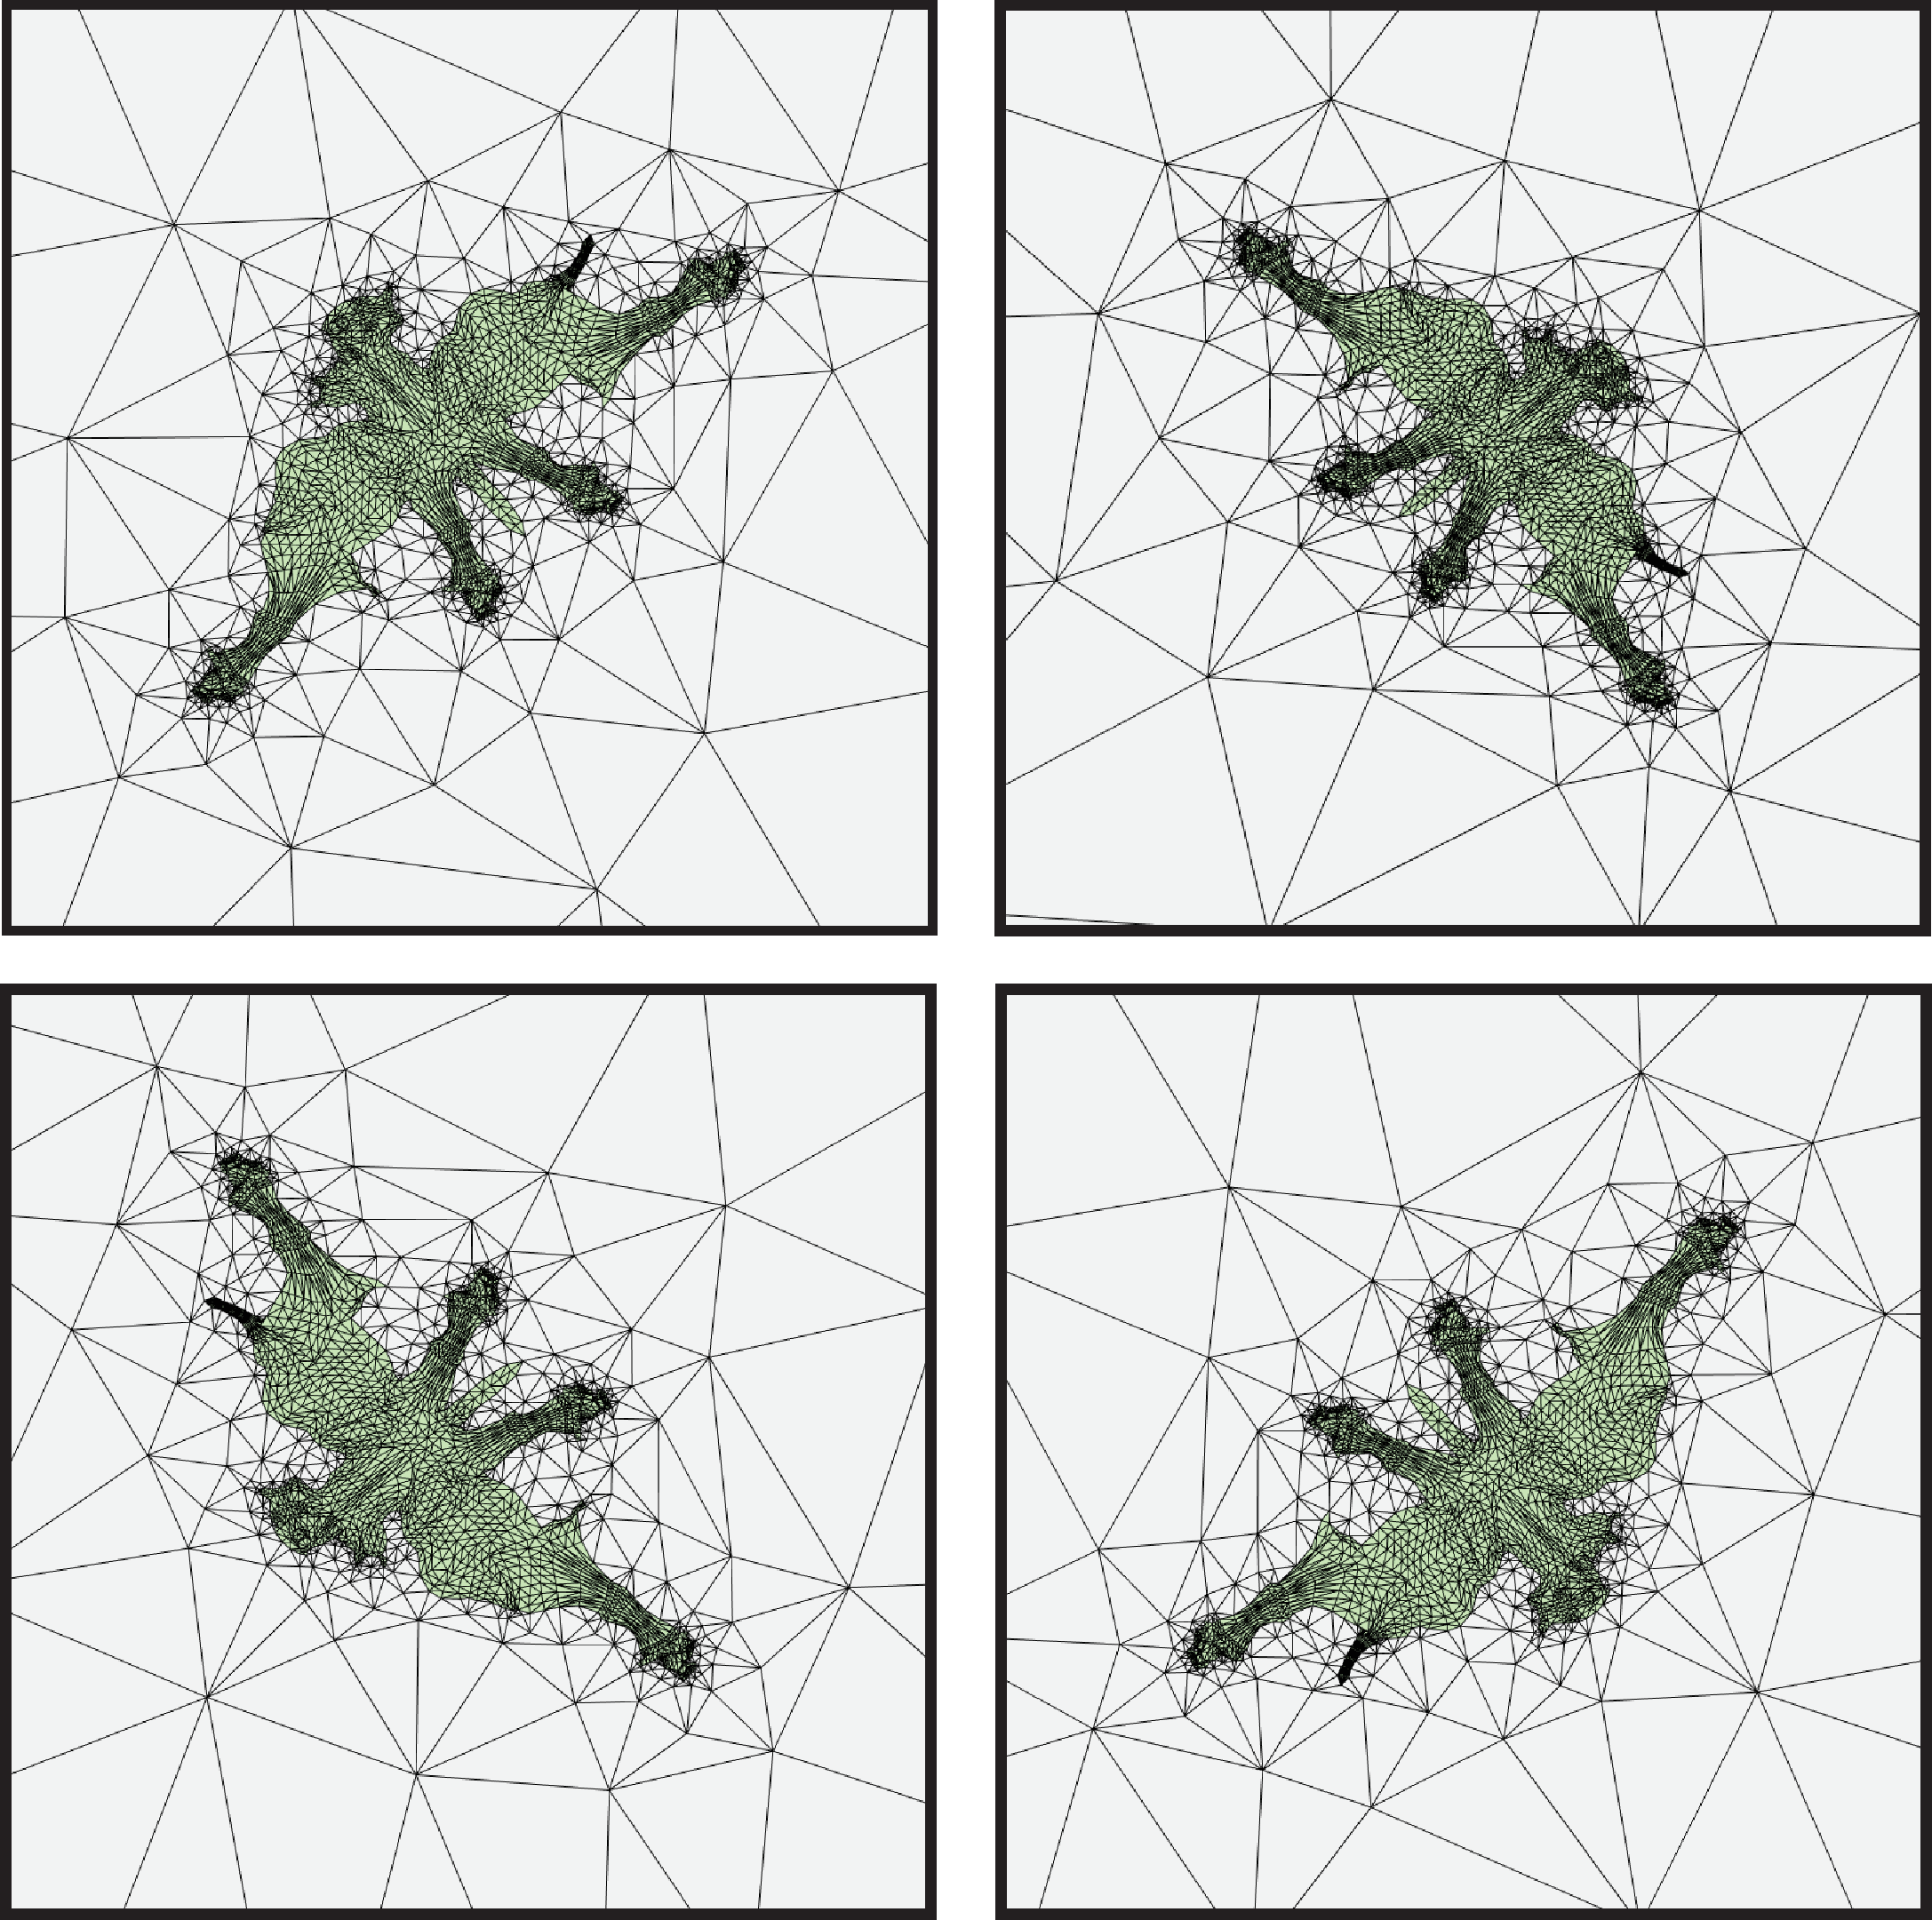
\includegraphics[width=\columnwidth]{figs/random-rotate.pdf}
\caption{
\revise{Our algorithm is independent to the initial orientation. We rotate the initializing Tutte's mapping of the camel model and obtain results with similar isometric distortion.}}
\vspace{-0.2cm}
\label{scaf:fig:random-rotate}
\end{figure}


\paragraph{Timings} The timings for all the results in the paper are reported in Table \ref{tab:timings}.
\begin{table}[t]
	\centering
	\begin{adjustbox}{width=\columnwidth,totalheight=\textheight,keepaspectratio}
	\begin{tabular}{llrrrrrrr}
%		\hline
\textbf{{Type}} &\textbf{Model} & $\mathbf{\#V}$	& $\mathbf{\#F}$ & $\mathbf{\#V_S}$	& $\mathbf{\#F_S}$ & \textbf{It.} & \textbf{{Total Time (s)}} & \textbf{{It. Time (s)}}\\
\hline
\multirow{2}{*}{Atlas}&Nefertiti (Fig.~\ref{scaf:fig:teaser})
&1697	&2823	&983/	247&	1945	/728&	50&	0.71&0.01\\
&Maneki-Neko (Fig.~\ref{scaf:fig:packing2D})
&23025	&43648	&2427	/725&	7174/	3770&	50&	16.81&0.34\\
\hline
\multirow{12}{*}{2D}
&Hand (Fig.~\ref{scaf:fig:different_weight})
&2239&4046&347/280&1104/970&7&0.14&0.02\\
&Spiral (Fig.~\ref{scaf:fig:recovering})
&54&52&78/36&190/106&50(50)&0.04(0.21)&0.01\\
&Thai Statue (Fig.~\ref{scaf:fig:miq_database}, left)
&42405&79970    &   3665/1593&12148/8004&50&28.28&0.56\\
&Filigree (Fig.~\ref{scaf:fig:miq_database}, right)
&56062&100000&9160/2627&30422/17356&100&75.99&0.76\\
&Lucy (Fig.~\ref{scaf:fig:scalability})&	501105&	1000000&	1856/	3470&	5900/	5674&	100&	2524.22&25.24\\
&Lucy (Fig.~\ref{scaf:fig:scalability})&	1001375&	1999999&	2284/	4400&	7297/	7133&	100&	7251.00&72.51\\
&Lucy (Fig.~\ref{scaf:fig:scalability})&	2002031&	3999999&	3587/	6930&	11215/	10985&	100&	22500.07&225.00\\
&Lucy (Fig.~\ref{scaf:fig:scalability})&	3002899&	5999999&	5135/	9859&	16047/	15601&	100&	52235.31&522.35\\
&Lucy (Fig.~\ref{scaf:fig:scalability})&	4002816&	8000000&	5140/	10288&	15890/	15918&	100&	59413.14&594.13\\
&Lucy (Fig.~\ref{scaf:fig:scalability})&	5003408&	10000000&	6194/	12231&	19182/	19040&	100&	95247.59&952.47\\
&Lucy (Fig.~\ref{scaf:fig:scalability})&6004111&12000000 & 7357/6418 & 2291/21036 &50 & 78726.05 &1574.52\\
&Animal (Fig.~\ref{scaf:fig:manuallycut})
&19937&39040&747/593&2306/1998&50&15.36&0.31\\
&Space Filling (Fig.~\ref{scaf:fig:smith})
&79545&146832&90815/88237&181608/176452&200(250)&547.13(1836.58)&5.30\\
&Horse (Fig.~\ref{scaf:fig:smith-all}) & 20636 & 39698 & 1343/984 & 4238/3520 & 30(10) & 8.26(12.03) & 0.28(1.20) \\
&Camel (Fig.~\ref{scaf:fig:smith-all}) & 2032 & 3576 & 384/272 & 1234/1010 & 30(10) & 0.52(1.13) & 0.02(0.11) \\
&Cow (Fig.~\ref{scaf:fig:smith-all}) & 3195 & 5804 & 491/277 & 1546/1118 & 30(10) & 0.81(1.74) & 0.03(0.17) \\
&Tricera (Fig.~\ref{scaf:fig:smith-all}) & 3163 & 5660 & 544/329 & 1732/1302 & 30(10) & 0.83(1.77) & 0.03(0.18) \\
\hline

\multirow{2}{*}{3D}&Leg (Fig.~\ref{scaf:fig:flow})
&6617&13230&5016/5021&68521/68544&500&3251.17&6.50\\
&Bunny (Fig.~\ref{scaf:fig:rabbit})
&568&1132&683/706&6209/6289&50&7.16&0.14\\

\hline
	\end{tabular}
	\end{adjustbox}
			\caption{Timings and statistics for the models shown in the paper. From left to right: number of input vertices and simplices, number of initial/final scaffold vertices and simplices, number of iterations, running time in seconds. The numbers in parenthesis refer to the Newton optimization. Note that our timings are considerably higher than those reported in the SLIM paper for the Lucy model since we used the reference implementation in \protect\cite{libigl}, which {does not use} a multi-threaded solver.}
	\label{tab:timings}
	\vspace{-0.2cm}
\end{table}


%\newpage
\section{Limitations and Concluding Remarks}

We proposed a simple and robust algorithm to generate bijective maps, both in 2D and 3D. We demonstrated the practical value of the algorithm in UV mapping and deformation applications, and its robustness with extensive stress tests.

One major venue for future work is the support of hard positional constraints, which are favored over soft constraints in many practical applications. Our current algorithm only supports soft constraints as geometric energy \cite{Schuller:2013}. To support hard constraints we would need to generate a bijective starting point that guarantees those constraints, and then preserve them in our optimization. While bijecive maps with hard constraints can be constructed for a 2D patch homeomorphic to a disk \cite{Weber:2014} and for a 3D volume homeomorphic to a ball \cite{Campen:2016}, the generic solution is still elusive.

In 3D cases, the generation of the initial scaffold is not as robust as in 2D, since TetGen fails for geometries with self-intersections and other imperfections. Our algorithm is also slower in 3D due to larger and denser linear systems, as well as the need for local mesh refinement operations instead of regenerating the entire tetrahedralization. We believe a more optimized and parallel implementation could reduce this overhead, and plan to explore this in the future.
%\vspace{-0.5em}

%slow in 3D\\
%no robust tetrahedralization\\
%no robust initialization\\
%satisfy user-constraints exactly\\
%floating point accuracy locking\\ % we address this with exact predicates, right?
%restricting to rotation-invariant energies\\
%some effect of the scaffold on the map\\  % we kind of already talk about this wrt sliding, mention again?
%minimal separation\\



 \begin{acks}
 The authors would like to thank
 Michael Rabinovich and Roi Poranne for providing the source code and Lucy models for \cite{Rabinovich:2017},
 Leonardo Sacht for providing the source code and Leg model for \cite{Sacht:2013},
 and the anonymous reviewers for their insightful comments and suggestions.
\end{acks}


\chapter{Bijective Projection in the Shell}
\label{chp:shell}


\begin{figure}
	\centering
	\includegraphics[width=\linewidth,draft=false]{prism-tex/figs/teaser_edit.pdf}
    \caption{A low-quality mesh with boundary conditions (a)
    is remeshed using our shell (b)
    to maintain a bijection between the input and the remeshed output.
    The boundary conditions (arrows in (a)) are then transferred to the high-quality surface (c),
    and a non-linear elastic deformation is computed %with PolyFEM%TODO
    on a volumetric mesh created with TetGen ({e}).
    The solution is finally transferred back to the original geometry ({d}).
    Note that in this application setting both surface and volumetric meshing {can be hidden from} the user, {who} directly specifies boundary conditions and analyses the result on the input geometry.}
    
    % \vspace{-1em}
    \label{prism:fig:teaser}
\end{figure}

\section{Introduction}
\label{prism:sec:introduction}

Triangular meshes are the most popular representation for discrete surfaces, due to their flexibility, efficiency, and direct support in rasterization hardware. Different applications demand different meshes, ranging from extremely coarse for collision proxies, to high-resolution and high-quality for accurate physical simulation.
%
For this reason, the adaptation of a triangle mesh to a specific set of criteria (surface remeshing) is a core building block in geometry processing, graphics, physical simulation, and scientific computing.

In most applications, the triangular mesh is equipped with attributes, such as textures, displacements, physical properties, and boundary conditions (Figure~\ref{prism:fig:teaser}). Whenever remeshing is needed, these properties must be transferred on the new mesh, a task which has been extensively studied in the literature and for which robust and generic solutions are still lacking (Section \ref{prism:sec:related}). 
Defining a {continuous} bijective map, {more precisely, a homeomorphism where the inverse is also continuous,} between two {geometrically close}  piecewise-linear meshes of the same topology is a difficult problem, even in its basic form, when one of these meshes is obtained by adapting the other in some way (e.g., coarsening, refining, or improving triangle shape).a
Common approaches to this problem are Euclidean projection
\cite{jiao2004overlaying}, parametrization on a common domain \cite{praun2001consistent,kraevoy2004cross,lee1998maps}, functional maps \cite{Ovsjanikov:2012}, and generalized barycentric coordinates \cite{Hormann:2017:GBC}.  However, the problem is not fully solved, as all existing methods, as we discuss in greater detail in Section~\ref{prism:sec:related},
 often fail to achieve bijectivity and/or sufficient quality of the resulting maps when applied to complex geometries. %geometrical models.
{Our focus is on correspondences between meshes obtained during a remeshing procedure, instead of solving the more general problem of processing arbitrary mesh pairs.}

In this work, we propose a general construction designed to enable attribute mapping between geometrically close (in a well-defined sense) meshes by jointly constructing: (1) a shell $\S$ around triangle mesh $\T$ spanned by a set of prisms, inducing a volumetric vector field $\V$ in its interior and (2) a projection operator $\P$ that bijectively maps surfaces inside the shell to $\T$, as long as the dot product of the surface face normals and $\V$ is positive
(we call such a surface a \emph{section} of $\S$).
Given a surface mesh $\T$ and its shell $\S$, it is now possible to exploit the bijection induced by $\P$ in many existing remeshing algorithms by adding to them an additional constraint ensuring that the generated surface is a section of a given shell.

As long as the generated mesh is a section, the projection operator $\P$ can be used to transfer application-specific attributes. At a higher level, the middle surface of our shell can be seen as a common parametrization domain shared by sections within the shell: differently from other methods that map the triangle meshes to a disk, region of a plane, a canonical polyhedron, or orbifolds, our construction uses an explicit triangle mesh embedded in ambient space as the common parametrization domain.
This provides additional flexibility since it is adaptive to the density of the mesh and naturally handles models with high genus, while being numerically stable under floating-point representation (and exact if evaluated with rational arithmetic). The downside is that it is defined only for sections contained within the shell. {
    The construction and optimization of our shell, and corresponding bijective mapping, is computationally more expensive than remeshing-only methods: our algorithms takes seconds to minutes on small and medium sized models, and might take hours on the large models in our tests.}

We evaluate the robustness of {the proposed}approach by constructing shells for a subset of the models in Thingi10k \cite{zhou2016thingi10k} and in ABC \cite{koch2019abc} (Section \ref{prism:sec:results}). We also integrate it in six common geometry processing algorithms to demonstrate its practical applicability (Section \ref{prism:sec:applications}):
\begin{enumerate}
    \item \emph{Proxy}.
    The creation of a proxy, high-quality remeshed surface to solve PDEs (e.g., to compute geodesic distances or deformations), avoiding the numerical problems caused by a low-quality input in commonly used codes.
%    without requiring any change in existing codes,
    Bijective projection operators associated with a shell enable us to transfer boundary conditions to the proxy mesh, compute the solution on the proxy, and then transfer the solution back to the original geometry.
    \item \emph{Boolean operations.} The remeshing of intermediate results of Boolean operations, to ensure high-quality intermediate meshes while preserving a bijection to transfer properties between them.
    \item \emph{Displacement Mapping.} The automatic conversion of a dense mesh into a coarse approximation and a regularly sampled displacement height map. Our method generates a  bijection that allows us to bake the geometric details in a displacement map.
    \item \emph{Tetrahedral Meshing.} The conversion of a surface mesh of low quality into a high-quality tetrahedral mesh, with bijective correspondence.
    \item \emph{Geometric Textures.} Generation of complex topological structures using volumetric textures mapped to the volumetric parametrization of a simplified shell defined by $\P$. Our analysis on the initial shell also complements the literature on shell maps.
    \item \emph{Nested Cages.} A robust approach to generate a coarse approximation of a surface for collision checking, cage-based deformation, or multigrid approaches.
\end{enumerate}

Our contributions are:
\begin{enumerate}
    \item An algorithm to build a prismatic shell and the corresponding projection operator around an orientable, manifold, self-intersection free triangle mesh with arbitrary quality;
    \item A new definition of bijective maps between {\emph{close-by} discrete} surfaces;%, closed under rational representation and at the same time efficient and robust to evaluate in floating-point;\ZJ{Not shown}
    \item A reusable, reference implementation {provided at \url{https://github.com/jiangzhongshi/bijective-projection-shell}}.
\end{enumerate}

\begin{figure}
    \centering
    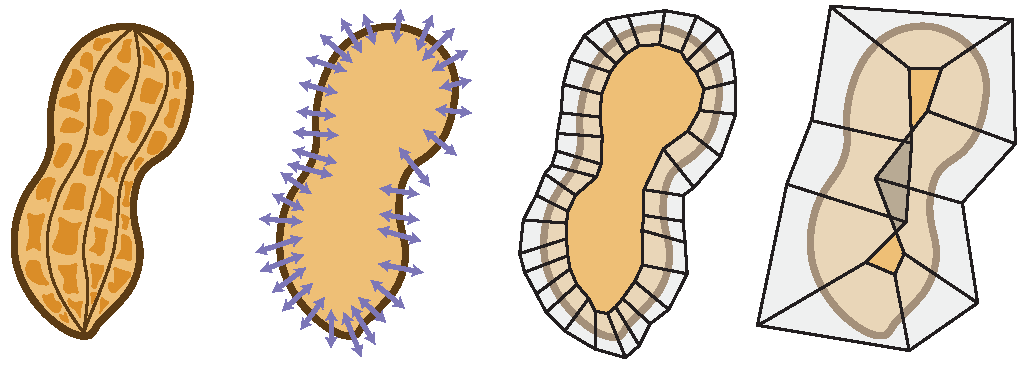
\includegraphics[width=\linewidth]{prism-tex/figs/pipeline}
    \caption{Overview of our algorithm. We start from a triangle mesh, find directions of extrusion, build the shell, and optimize to simplify it.}
    \label{prism:fig:pipeline}
    
\end{figure}

\section{Method}\label{prism:sec:method}
Our algorithm (Figure~\ref{prism:fig:pipeline}) converts a self-intersection free, orientable, manifold triangle mesh $\T = \{V_\T,F_\T\}$, where $V_\T$ are the vertex coordinates and
$F_\T$ the connectivity of the mesh, into a shell composed of generalized prisms $\S = \{(B_\S,M_\S,T_\S),F_\S\}$, where $B_\S$, $M_\S$, $T_\S$ are bottom, middle, and top surfaces of the shell, 
consisting of bottom, middle, and top  triangles of the prisms,
and $F_\S$  is the connectivity of the prisms (Figure \ref{prism:fig:corona}).
The algorithm initially generates a shell $\S$ whose middle surface $M_\S$ has the same geometry as the input surface $\T$ (possibly with refined connectivity),
and then optimizes it while ensuring that $\T$ is contained inside and projects bijectively to $M_\S$. The shell induces a volumetric vector field $\V$ and a projection operator $\P$ in the interior of each of its prisms (Section \ref{prism:sec:projection}). This output can be used directly in many geometry processing tasks, as we discuss in detail in Section~\ref{prism:sec:applications}.

\begin{figure}
    \centering
    \includegraphics[width=0.9\linewidth]{prism-tex/figs/corona}
    \caption{Example of the top (left, outer) and bottom (right, inner) surface of the prismatic shell.}
    
    \label{prism:fig:corona}
\end{figure}


We first introduce the definition of our projection operator $\P$ and the conditions required for bijectivity of its restrictions to sections of the shell (Section \ref{prism:sec:projection}). We then define shell validity (Section \ref{prism:sec:strong}), present our algorithm for creating an initial shell (Section\ \ref{prism:sec:initialization}) and optimizing it to decrease the number of prisms (Section \ref{prism:sec:optimization}).
To simplify the exposition,
we initially assume that our input triangle mesh does not contain \emph{singular points} (defined in Section~\ref{prism:sec:initialization}) and boundary vertices, and we explain how to modify the algorithm to account for these cases in sections \ref{prism:sec:singularities} and \ref{prism:sec:boundaries}.

\subsection{Shell and Projection}
\label{prism:sec:projection}

Let us consider a single generalized prism $\Prism$ in a prismatic layer $\S$ (Figure \ref{prism:fig:prism_decomposition} left). The generalized prism $\Prism$ is defined by the position of the vertices of three triangles, one at the top, with coordinates $t_1,t_2,t_3$, one at the bottom, with coordinates $b_1,b_2,b_3$, and one in the middle, implicitly defined by a per-vertex parameter $\alpha_i \in [0, 1]$, with coordinates $m_i = \alpha_i t_i + (1-\alpha_i) b_i, i=1,2,3$. We will call the top (bottom) ``half'' of the prism \emph{top (bottom) slab} (we refer to Appendix~\ref{app:dblayer} for an explanation on why we need two slabs).
For brevity, we will refer to a generalized prism as a prism.

% Without loss of generality, we will describe our algorithm only for the top half of the prism $\Prism$ denoted $\H$ since the other half of the construction is symmetric.

\begin{figure}
    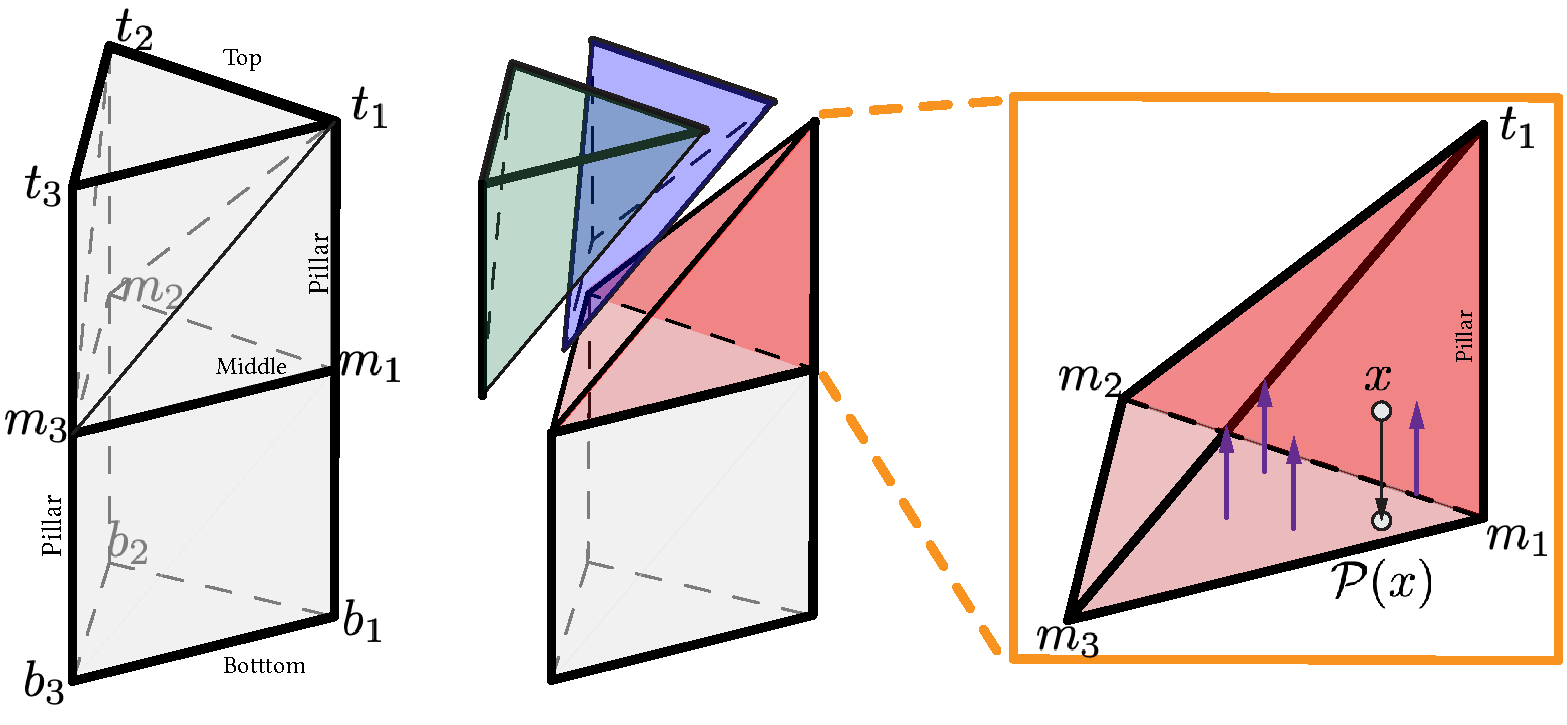
\includegraphics[width=\linewidth]{prism-tex/figs/prism_projection}
    \caption{A prism $\Prism$ (left) is decomposed into 6 tetrahedra (middle, for clarity, we only draw the 3 tetrahedra of the top slab). Each tetrahedron has a constant vector field in its interior (pointing toward the top surface), which is parallel to the only pillar of the prism that contains the point.}
    \label{prism:fig:prism_decomposition}
    
\end{figure}

 \paragraph{Decomposition in Tetrahedra} We decompose each prism $\Prism$ into 6 tetrahedra (3 in the top slab and 3 in the bottom one, Figure~\ref{prism:fig:prism_decomposition} middle), using one of the patterns in \cite[Figure 4]{dompierre1999subdivide}. The patterns are identified by the orientation (rising/falling) of the two edges cutting the side faces of the prism. While, for a single prism, any decomposition would be sufficient for our purposes, we need a consistent tetrahedralization between neighboring prisms to avoid inconsistencies in the projection operator. To resolve this ambiguity, we use the technique proposed in \cite{garimella2000boundary}: we define a total ordering over the vertices of the middle surface of $\Prism$ (naturally, we use the vertex id) and split (for each half of the prism) the face connecting vertices $v_1$ and $v_2$ with a rising edge if $v_1 < v_2$ and a falling edge otherwise. 

\paragraph{Forward and Inverse Projection}
% \ZJ{multi-value definition comment.
% Vector Field is defined piecewise, but the projection is unique.}
We define a piecewise constant vector field $\V$ inside the decomposed prism,
by assigning to each tetrahedron $\Tet_j^{\Prism}$, $j=1,\hdots,6$,
the constant vector field defined by the only edge of $\Tet_j^{\Prism}$ which is a \emph{oriented pillar} of $\Prism$ connecting the bottom surface to the top surface passing through the middle surface). That is, for any $p\in \Tet_j^{\Prism}$
\begin{equation}
    \label{eq:V}
    \V(p) = t_i - b_i,
\end{equation}
where $i$ is the index of the vertex corresponding to the pillar edge of $\Tet_j^{\Prism}$.
Note that {$\V$ is constant on each tetrahedron and might be discontinuous on the boundary: we formally define the value of $\V$ on the boundary as any of the values of the incident tetrahedra. This choice does not affect our construction.}
{T}here is exactly one {integral (poly-)line} passing through each point of the prism if
all the decomposed tetrahedra have positive volumes
(Theorem~\ref{thm:projection}). This allows us to define
the \emph{projection operator} $\P(p)$ for a point $p \in \Prism$ as the intersection of the {integral line} $f_p(t)$ of the vector field $\V$ passing through $p$, with the middle surface of $\Prism$ (Figure~\ref{prism:fig:advection}). 
%
\begin{figure}
    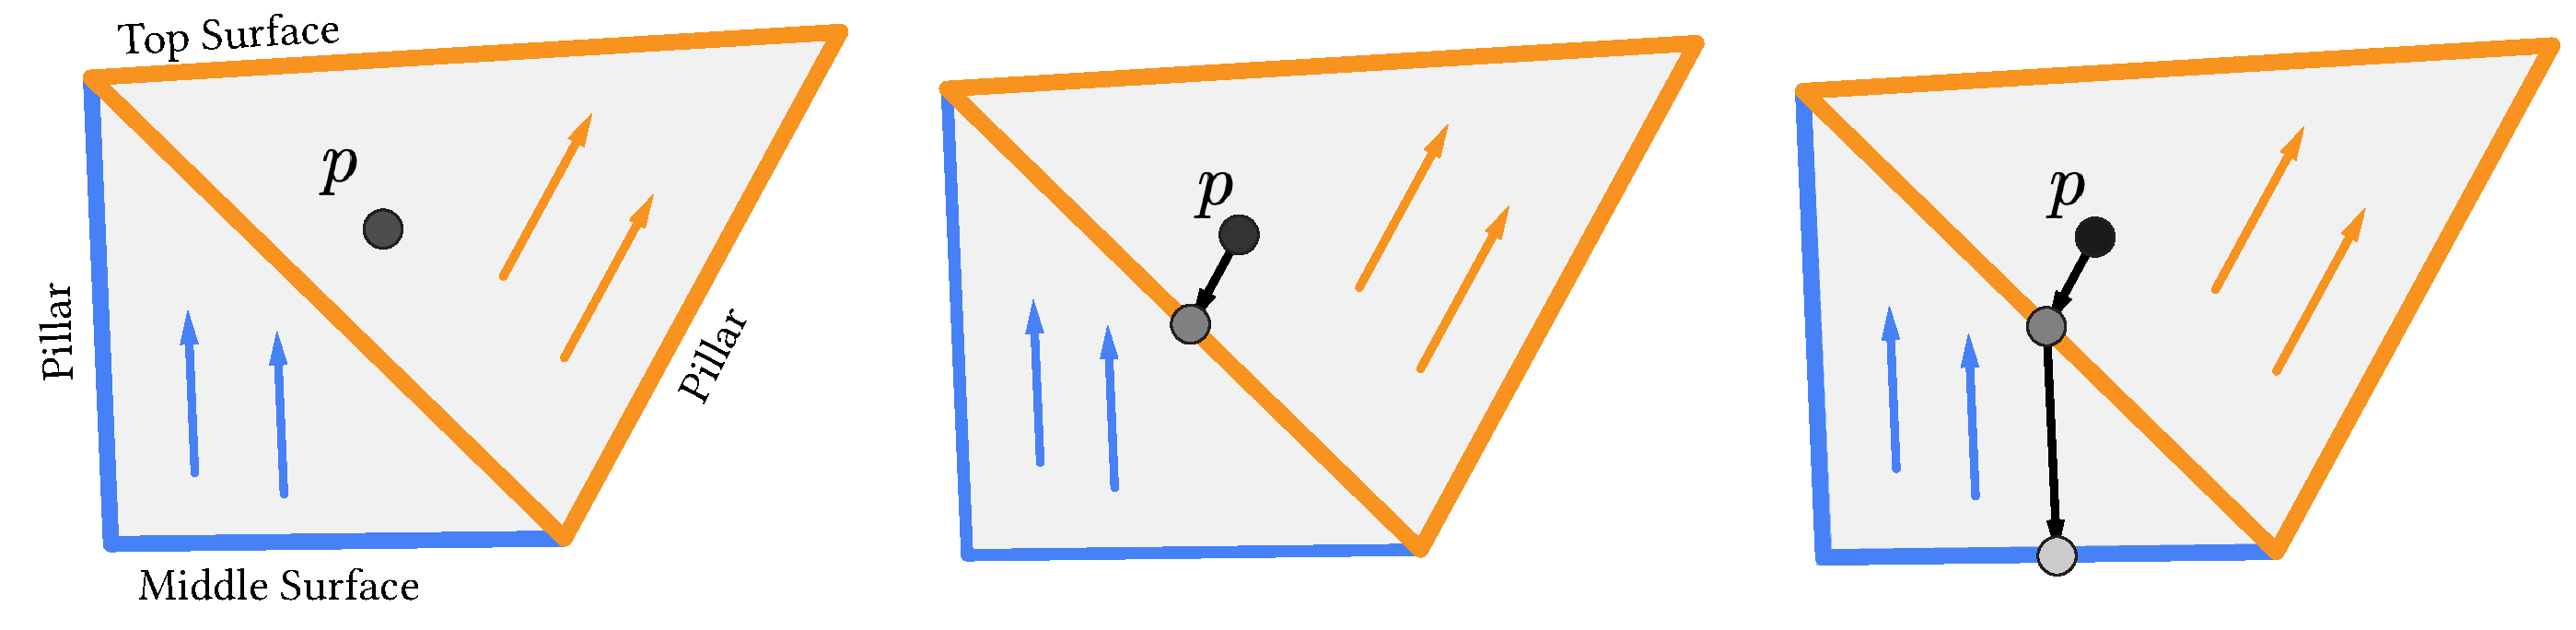
\includegraphics[width=\linewidth]{prism-tex/figs/projection}
    \caption{A point $p$ (left) is traced through $\V$ inside the top part of the shell. A ray with $p$ as origin and $\V$ as direction is cast inside the orange tetrahedron (middle). The procedure is repeated (on the blue tetrahedron) until the ray hits a point in the middle surface (right).}
    \label{prism:fig:advection}
    
\end{figure}
%
% \begin{wrapfigure}{r}{width=0.3\linewidth}
%     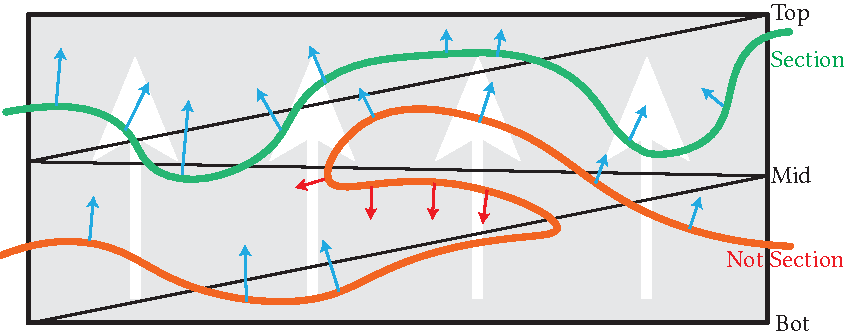
\includegraphics[width=\linewidth]{prism-tex/figs/not-section-illustrate}
% \caption{Example of being a section (green) and not a section (red).}
% \end{wrapfigure}
%
Intuitively, we can project any mesh that does not fold in each prism (Figure~\ref{prism:fig:not_section}) to the middle surface.
\begin{figure}
    \centering
    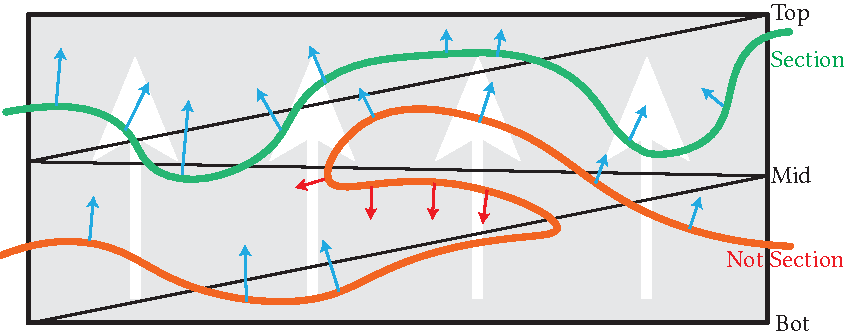
\includegraphics[width=0.8\linewidth,draft=false]{prism-tex/figs/not-section-illustrate}
    \caption{A 2D illustration for the normal dot product condition. The blue arrows agrees with the background vector field (white arrows), while the red arrows do not agree.}
    \label{prism:fig:not_section}
    
\end{figure}
Formally, we introduce the following definition, to describe this property in terms of the triangle normals of the mesh.

With a slight abuse of the notation, for meshes and collections of prisms $A$ and $B$, we use $A \cap B $ to denote the intersection of their corresponding geometry.

\begin{definition}
\label{def:section}
A \emph{section} $\hat{\T}$ of a prism $\Prism$ is a manifold triangle mesh whose intersection with $\Prism$ is a simply connected submesh $\hat{\T} \cap \Prism$ whose single boundary loop is contained in the boundary of $\Prism$, excluding its top and bottom surface, and such that for every point $p \in \hat{\T} \cap \Prism$ the dot product
between the face normal $n(p)$ and the vector field $\V(p)$ is strictly positive. Similarly, a triangle mesh $\hat{\T}$ is a \emph{section of a shell $\S$}, if it is a section of all the prisms of $\S$.
\end{definition}
Note that this definition implies that all sections are contained inside the shell.
% that is, the union of all prisms minus the intersection region of non-adjacent prisms (light gray area in Figure~\ref{prism:fig:pipeline)}\ZJ{Move this sentence}.
{Additionally, the definition implies that the section does not intersect with either bottom or top surface. 
However, our definition allows for the bottom or top surface to self-intersect. 
The intersection of the shell does not invalidate the \emph{local} definition of projection since it is defined per prism.
Allowing intersections is crucial to an efficient implementation of our algorithm since it allows us to take advantage of a static spatial data structure in later stages of the algorithm (Section~\ref{prism:sec:optimization}).
}

 

\begin{theorem}
If all  6 tetrahedra $\Tet_j^{\Prism}$ in a decomposition of a prism $\Prism$ have positive volume,
then the projection operator $\P$ defines a bijection between any section $\hat{\T}$ of $\Prism$ and the middle triangle of the prism ($M$ in Figure~\ref{prism:fig:projection_sections}).
\label{thm:projection}
\end{theorem}
\begin{proof}
    \label{app:projection}
    Consider the unique (up to symmetry) piece-wise affine map $T$ deforming $\Prism$ into a reference prism $\hat\Prism = \{u,v \geq 0|u+v \leq 1\} \times [-1,1]$, identifying the bottom surface of $\hat\Prism$ as $z=-1$, middle surface as $z=0$, and top surface as $z=1$.
    Let $T_{\Tet}$ be the affine map mapping tetrahedron $\Tet$ to the reference prism.
    Since the volume of all $\Tet$ is positive by assumption, the map $T$ is bijective and orientation preserving. 
    In particular, $T$ transforms $\V(p)$ to the const vector $e_z = (0,0,1)$ since the edges of the prism are mapped to axis aligned edges of the reference prism. The projection operator $\P(p)$ can thus be equivalently defined as $\P(p) = T^{-1}(\P_z(T(p)))$, where $\P_z$ is the projection over the $z$-axis in the reference prism. 
    $\P_z$ is bijective if the piecewise linear mesh intersecting $\Prism$ is composed of triangles with positive area (and the boundaries are mapped to the boundaries) \cite{lipman2014bijective}, after being mapped to the reference $\Prism$ and projected by $\P_z$. In the reference domain, having positive area after projection (with a fixed boundary) is equivalent to that the dot product between the projection direction and the normal of every face is positive. In the top half of $\Prism$, $\P_z$ is bijective if for every point $T(p), p \in f$ $T(n_p)\cdot [0,0,1] = T(n_p) \cdot T(\V(p)) > 0$  which holds since $ n_p \cdot \V(p) > 0$ (from the definition of section) and the fact that $T$ is orientation preserving and thus not changing the sign of the dot product.
\end{proof}

The \emph{inverse projection operator} $\P^{-1}$ is defined for a section $\hat{\T}$ as the inverse of the forward projection
restricted to $\hat{\T}$. %, $\P: \hat{\T} \rightarrow \T$ is bijective.
It can be similarly computed by tracing the vector field in the opposite direction, starting from a point in the middle surface of the prism. Note that, differently from the inverse Phong projection \cite{panozzo2013weighted, kobbelt1998interactive}, whose solution depends on the root-finding of a quadric surface, our shell has an explicit form for the inverse and does not require a numerical solve. The combination of forward and inverse projection operators allows to bijectively map between any pair of sections, independently of their connectivity (Figure \ref{prism:fig:projection_sections}). An interesting property of our forward and inverse projection algorithm, which might be useful for applications requiring a provably bijective map, is that our projection could be evaluated exactly using rational arithmetic.

%%%%%%%%%%

\begin{figure}
    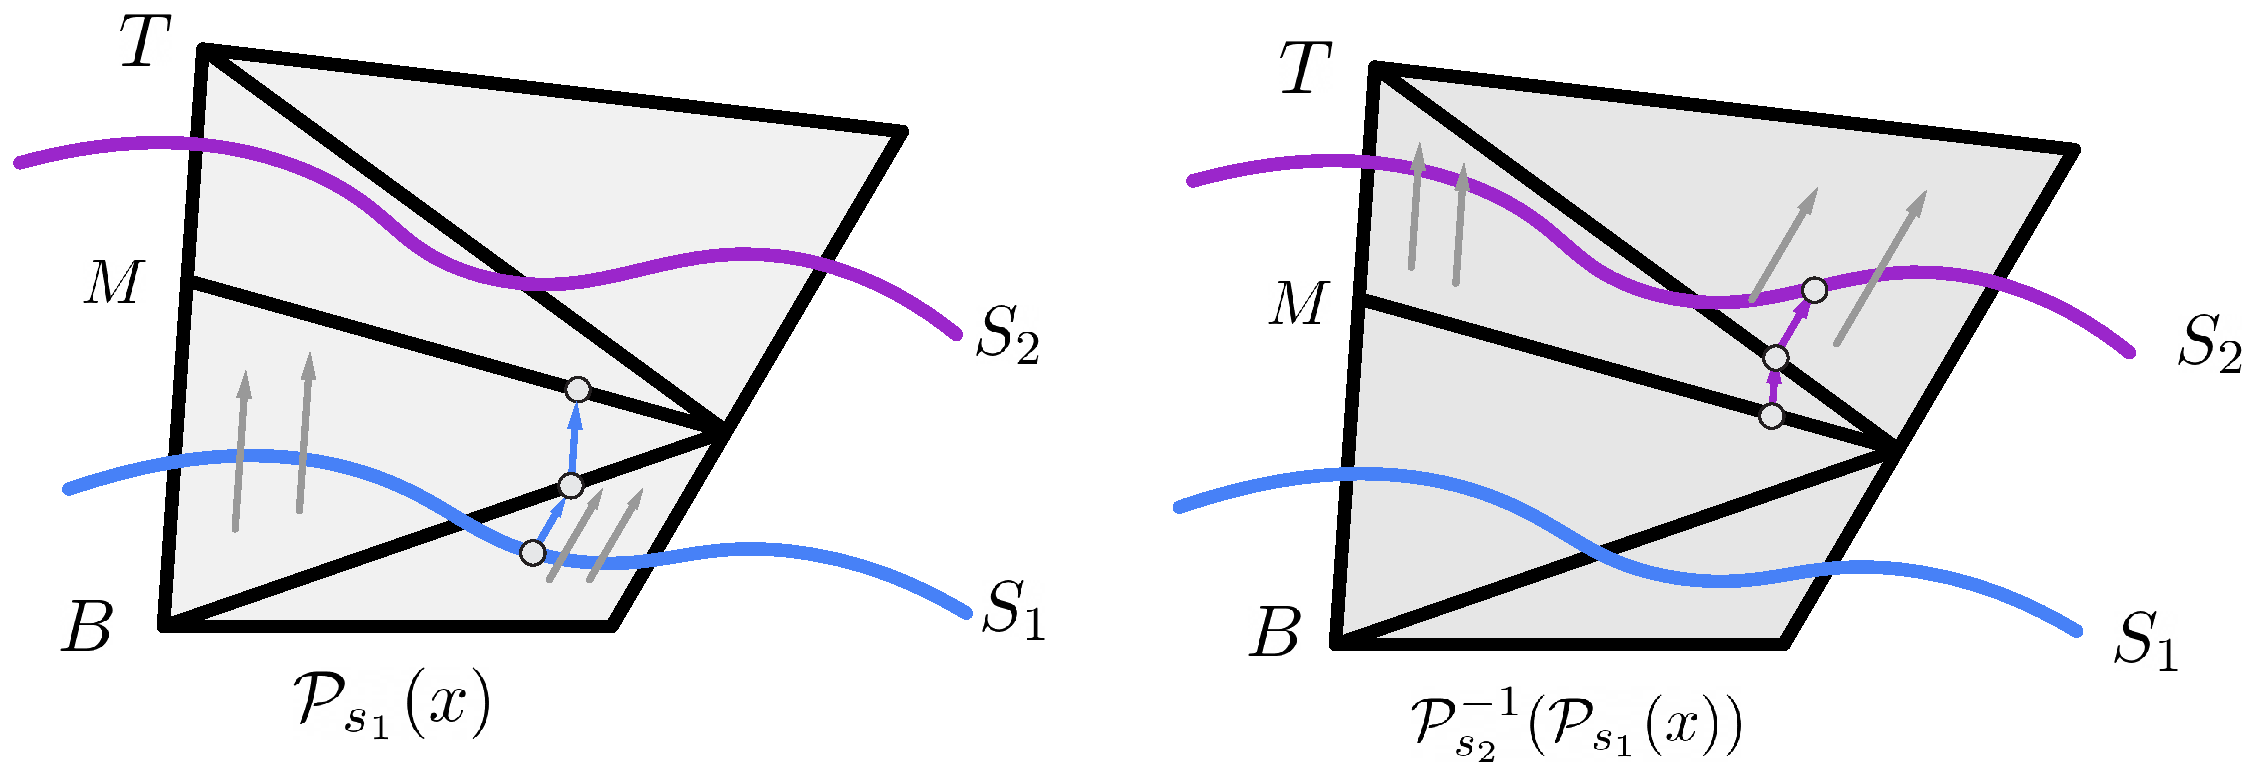
\includegraphics[width=\linewidth]{prism-tex/figs/composition}
    \caption{The composition $\P^{-1}_{\S_2}(\P_{\S_1}(x))$ with $x \in \S_1$, of a direct and an inverse projection operator defines a bijection between two sections $\S_1$ and $\S_2$.}
    \label{prism:fig:projection_sections}
    
\end{figure}

{
\subsection{Validity Condition}
\label{prism:sec:strong}

Shell, projection operator, section definitions, and the bijectivity condition (Theorem~\ref{thm:projection}) are dependent on a specific tetrahedral decomposition, which depends on vertex numbering.

To ensure that our shell construction is independent from the vertex and face order, we define the validity of a shell by accounting for all 6 possible tetrahedral decompositions \cite[Figure 4]{dompierre1999subdivide}}.

\begin{definition}\label{def:validshell}
% \paragraph{Validity}
We say that a prismatic shell $\S$ is \emph{valid with respect to a mesh $\hat\T$} if it satisfies two conditions for each prism.
\begin{enumerate}
    \item[I1] \emph{Positivity}. The volumes of  24 tetrahedra (Appendix \ref{app:I1}) corresponding to  6 tetrahedral decompositions are positive.
    \item[I2] \emph{Section.} $\hat\T$ is a section of $\S$ for all 6 decompositions.
\end{enumerate}
\end{definition}
If a shell is valid, from I1, I2, then by Theorem \ref{thm:projection}, it follows that any map between sections induced by the projection operator $\P$ is bijective.

I2 ensures that the input mesh is a \emph{valid section} independently from the decomposition, that is, we require the dot product to be positive with respect to all \emph{three} pillars of a prism inside the convex hull. An interesting and useful side effect of this validity condition is that it ensures the bijectivity of a natural nonlinear parametrization of the prism interior (Appendix \ref{app:bilinear}, Figure~\ref{prism:fig:displacement-mapping}).

\subsection{Shell Initialization}
\label{prism:sec:initialization}

We now introduce an algorithm to compute a \emph{valid} prismatic shell $\S = \{(B_\S,M_\S,T_\S),F_\S\}$ with respect to a given triangle mesh $\T = \{V_\T,F_\T\}$ such that $\T$ is geometrically identical to the middle surface of $\S$.  We assume that the faces of the triangle mesh are consistently oriented.

\paragraph{Extrusion Direction.} The first step of the algorithm is the computation of an extrusion direction for every vertex of $\T$. These directions are optimized to be pointing towards the \emph{outside} of the triangle mesh (which we assume to be orientable), that is,
they must have a positive dot product with the normals of all incident faces. More precisely, for a vertex $v$, we are looking for a direction $d_v$ such that $d_v \cdot n_f > 0$ for each adjacent face $f$ with normal $n_f$. We can formulate this as the optimization problem
\begin{equation}
\label{eq:OPT}
\begin{split}
    \max_{d_v}& \min_{f \in N_v} n_f \cdot d_v,\\
    \text{s.t. }&\quad n_f \cdot d_v \geq {\epsilon}, \qquad \forall f \in N_v\\
               &\quad  \|d_v\|^2 = 1.
\end{split}
\end{equation}

With slack variable $t$, Problem \ref{eq:OPT} can be rewritten as

$$\max_t t;\; d_v n_f \geq t, \|d_v\| = 1, t \geq {\epsilon}.$$

In the admissible region, substituting 
$t = 1/s$, 
$$\min_s s;\; s d_v n_f \geq 1, \|d_v\| = 1, {0< s \leq 1/\epsilon}.$$
Substituting $x=s d_v$ (thus $\|x\| = s\|d\| = s$), we obtain the QP problem \ref{eq:QP}. Note that the lower bound on $s$ is implied from $s d_v n_f \geq 1$, and the upper bound $\|x\| < 1/\epsilon$ is checked a posteriori.

A solution, if it exists, can be found solving the following quadratic programming problem
\begin{equation}
\label{eq:QP}
\begin{split}
    \min&\quad \|x\|^2,  \\
    \text{s.t.}&\quad \mathbf{C} x \geq 1,
\end{split}
\end{equation}
with $d_v = x / \|x\|$ and $\mathbf{C}$ the matrix whose rows are the normals $n_f$ of the faces in the 1-ring $N_v$ of vertex $v$. Solutions not satisfying $\|x\| \leq 1/\epsilon$ needs to be discarded. The QP can be solved with an off-the-shelf solver\cite{osqp,cheshmi2020nasoq}, and in particular it can be solved exactly \cite{gartner2000efficient} to avoid numerical problems. Note that the Problem \eqref{eq:OPT} is studied in a similar formulation in~\cite{aubry2008most} but their solution requires tolerances in multiple stages of the algorithm to handle cospherical point configurations.




The admissible set of \eqref{eq:OPT} might be empty for a vertex $v$,
that is, no vector $d_v$ satisfies $\mathbf{C}d_v\geq\epsilon$. 
In this case we call $v$ a \emph{singularity}. For example, Figure \ref{prism:fig:singularity_example} shows a triangle mesh containing a singularity: there exist no direction whose dot product with the adjacent face normals is positive. To simplify the explanation, we assume for the remainder of this section that $\T$ does not contain singularities and also that it does not contain boundaries: we postpone their handling to sections \ref{prism:sec:singularities} and \ref{prism:sec:boundaries}.

\begin{proposition}\label{thm:I1}
Let $\T$ be a closed (without boundary) triangle mesh without singularities and $\N$ be a per-vertex displacement field satisfying $\mathbf{C} \N_i > 0$ for every vertex $v_i$ of $\T$. 
Then there exist a strictly positive per-vertex \emph{thickness} $\delta_i$ such that vertices $t_i$ and $b_i$ obtained by displacing $v_i$ by $\delta_i$ in the direction of $\N_i$ and in the opposite direction, define a shell that satisfies invariant I1.
\end{proposition}
\begin{proof}
    \label{app:I1}
    For simplicity, we will show that a uniform lower bound $\delta$ for all vertices exists. By consider a triangle of $T$, extruded over the displacement field $\N$, we obtain a generalized half prism with six vertices
    $0$, $e_1$, $e_2$, $\delta n_0$, $e_1$ + $\delta n_1$, $e_2 + \delta$ $n_2$, with $\delta$ a positive constant. The indices of the tetrahedra are:
    (0 ,2, 3, 4), 
    (0 ,3, 4, 5), 
    (0 ,1, 5, 3), 
    (0 ,1, 2, 3), 
    (1 ,2, 3, 4), 
    (0 ,1, 2, 4), 
    (0 ,1, 5, 4), 
    (1 ,3, 4, 5), 
    (1 ,2, 3, 5), 
    (0 ,2, 5, 4), 
    (0 ,1, 2, 5), 
    (2 ,3, 4, 5). 
    
    For a sufficiently small $\delta$, the linear term will dominate the higher power of $\delta$, which we omit. 
    The dominant volume terms are listed in the following table: ($e_{ij} := e_j - e_i$)
    
    \vspace{1em}
    {
    % \begin{table}[t]
    \footnotesize
    %     \centering
        {
    \begin{tabular}{|l|l|l|}
    \hline
    (0 ,2, 3, 4)&\text{vol1}$( 0,e_2,\delta  n_0,e_1 + \delta  n_1)           $&$ \delta \langle e_2,n_0,e_1\rangle$\\             
    (0 ,3, 4, 5)&\text{vol2}$( 0,\delta  n_0,e_1 + \delta  n_1,e_2 + \delta n_2)   $&$ \delta \langle n_0,e_1,e_2\rangle $\\
    (0 ,1, 5, 3)&\text{vol3}$( 0,e_1,e_2 + \delta n_2,\delta  n_0)            $&$ \delta \,\langle e_1,e_2,n_0\rangle  $\\
    (0 ,1, 2, 3)&\text{vol4}$( 0,e_1,e_2,\delta  n_0)                    $&$ \delta \langle e_1,e_2,n_0\rangle                           $\\
    (1 ,2, 3, 4)&\text{vol5}$( e_1,e_2,\delta  n_0,e_1 + \delta  n_1)         $&$ \langle e_{12}, \delta  n_0 - e_1, \delta n_1\rangle            $\\ 
    && $=\delta \langle e_2, -e_1, n_1\rangle     $\\
    (0 ,1, 2, 4)&\text{vol6}$( 0,e_1,e_2,e_1 + \delta  n_1)             $&$ \delta \langle e_1,e_2,n_1\rangle                             $\\
    (0 ,1, 5, 4)&\text{vol7}$( 0,e_1,e_2 + \delta n_2,e_1 + \delta  n_1)     $&$ \langle e_1,e_2 + \delta n_2, \delta  n_1\rangle                  $\\ 
    &&$ =\delta \langle e_1,e_2,n_1\rangle                                           $\\
    (1 ,3, 4, 5)&\text{vol8}$( e_1,\delta  n_0,e_1 + \delta  n_1,e_2 + \delta n_2) $&$ \delta \langle \delta  n_0 -e_1, n_1, e_{12} + \delta n_2\rangle    $\\ 
    &&$ = \delta \langle -e_1, n_1, e_2\rangle                                   $\\
    (1 ,2, 3, 5)&\text{vol9}$( e_1,e_2,\delta  n_0,e_2 + \delta n_2)          $&$ \langle e_{12}, \delta  n_0 - e_1, e_{12} + \delta n_2 \rangle $\\
    &&$ =\delta \langle e_{12}, \delta  n_0 - e_1, n_2\rangle $\\
    &&$ =\delta \langle e_2, - e_1, n_2\rangle $\\
    (0 ,2, 5, 4)&\text{vol10}$( 0,e_2,e_2 + \delta n_2,e_1 + \delta  n_1)     $&$ \delta \langle e_2, n_2, e_1\rangle$ \\
    (0 ,1, 2, 5)& \text{vol11}$( 0,e_1,e_2,e_2 + \delta n_2)$
                                                      &$ \delta \langle e_1,e_2,n_2\rangle $\\
    (2, 3, 4, 5)&\text{vol12}$( e_2,\delta  n_0,e_1 + \delta  n_1,e_2 + \delta n_2) $&$ \langle \delta  n_0 - e_2, \delta  n_1-e_{12}, \delta  n_2\rangle      $\\
    &&$ =\delta \langle - e_2, e_1, n_2\rangle$
                                                      \\
                                                      \hline
    \end{tabular}}
    % \end{table}
    \vspace{1em}
    }
    
    
    For all the 12 tetrahedra the linear term is multiplied by a determinant containing the edges of the prism. We check directly that all these determinants are positive due to the assumption that $\mathbf{C} \N_i > 0$.
    
\end{proof}




\paragraph{Initial Thickness}
We first show that a strictly positive per-vertex thickness $\delta$ exists for a shell $\S$ with $\T$ as its middle surface, and then discuss a practical algorithm to realize it.

\begin{theorem}
\label{thm:thickness}
Given a closed, orientable, self-intersection free triangle mesh $\T$ such that for all its vertices  Problem \eqref{eq:OPT} has a solution, a shell $\S$ exists such that $\T$ is the middle surface and there exist a strictly positive per-vertex thickness $\delta$.
\end{theorem}
\begin{proof}

    Consider a ball around a point $p$ of the middle face $M$ of the prism.  
    If the radius $r(p) > 0$ is sufficiently small, it contains, at most, a single vertex of $M$, and parts of incident  faces. As $M$ is compact, there is a minimal value of $r$ on $M$, and it is positive. 
    The line along the normal, passing through $v$, intersects incident faces at $v$ so it cannot intersect them at any other point. Thus, the top and bottom prism vertices can be obtained by displacing $V$ by $r$ in either direction along the normal. 
    Consider the $r$-neighborhood of the $M$, i.e. the union of all balls of radius $r$ centered at 
    points of $M$. This is a convex set, containing only $M$ and parts of vertex-adjacent faces. 
    All top and bottom prism vertices are in this set. Thus tetrahedra connecting these vertices are also in the set, i.e., complete prisms. The fact that tetrahedra are nondegenerate is established in Proposition~\ref{thm:I1}.
    \end{proof}


To find a valid per-vertex thickness $\delta_i$ to construct the top surface, we initially cast a ray in the direction of $\N$ for each vertex and measure the distance to the first collision with $\T$ (and cap it to a user-defined parameter $\delta_{max}$ if no collision is found).
An initial top mesh is built with this extrusion thickness; then we test whether any triangle in the top surface intersects $\T$, through triangle-triangle overlap test \cite{guigue2003fast},
and iteratively shrink $\delta_i$ in this triangle by 20\% until we find a thickness that prevents intersections between the input and the top surface. Analogously, we build the bottom shell along the opposite direction. {Note that the thickness of a vertex for the top and bottom surface can be different.}

\paragraph{Validity of the Initial Shell}
Proposition~\ref{thm:I1} and Theorem~\ref{thm:thickness} ensure that the initial shell constructed using a displacement field $\N$ obtained by solving \eqref{eq:QP}, satisfies property I1. However, $\T$ might not formally satisfy the conditions for being a section of $\S$, despite being identical to the middle surface of $\S$, due to our definition of the projection operator $\P$.
%
The reason for this can be seen in Figure \ref{prism:fig:closed}.
After the initialization, the middle surface is the input mesh. Thus every prism $\Prism$ corresponds to a triangle $T_\Prism$ of $\T$. The intersection $\Prism \cap \T$, required to check if $\T$ is a section of $\Prism$ (Definition \ref{def:section}) contains points from both $T_\Prism$ and its 1-ring neighborhood.

The projection operator (and thus the definition of the section) is based on all tetrahedral decompositions of $\Prism${;} it is possible that multiple tetrahedra (with different vector field values in $\V$) overlap on the boundary of $\Prism$. 


\begin{figure}\centering
    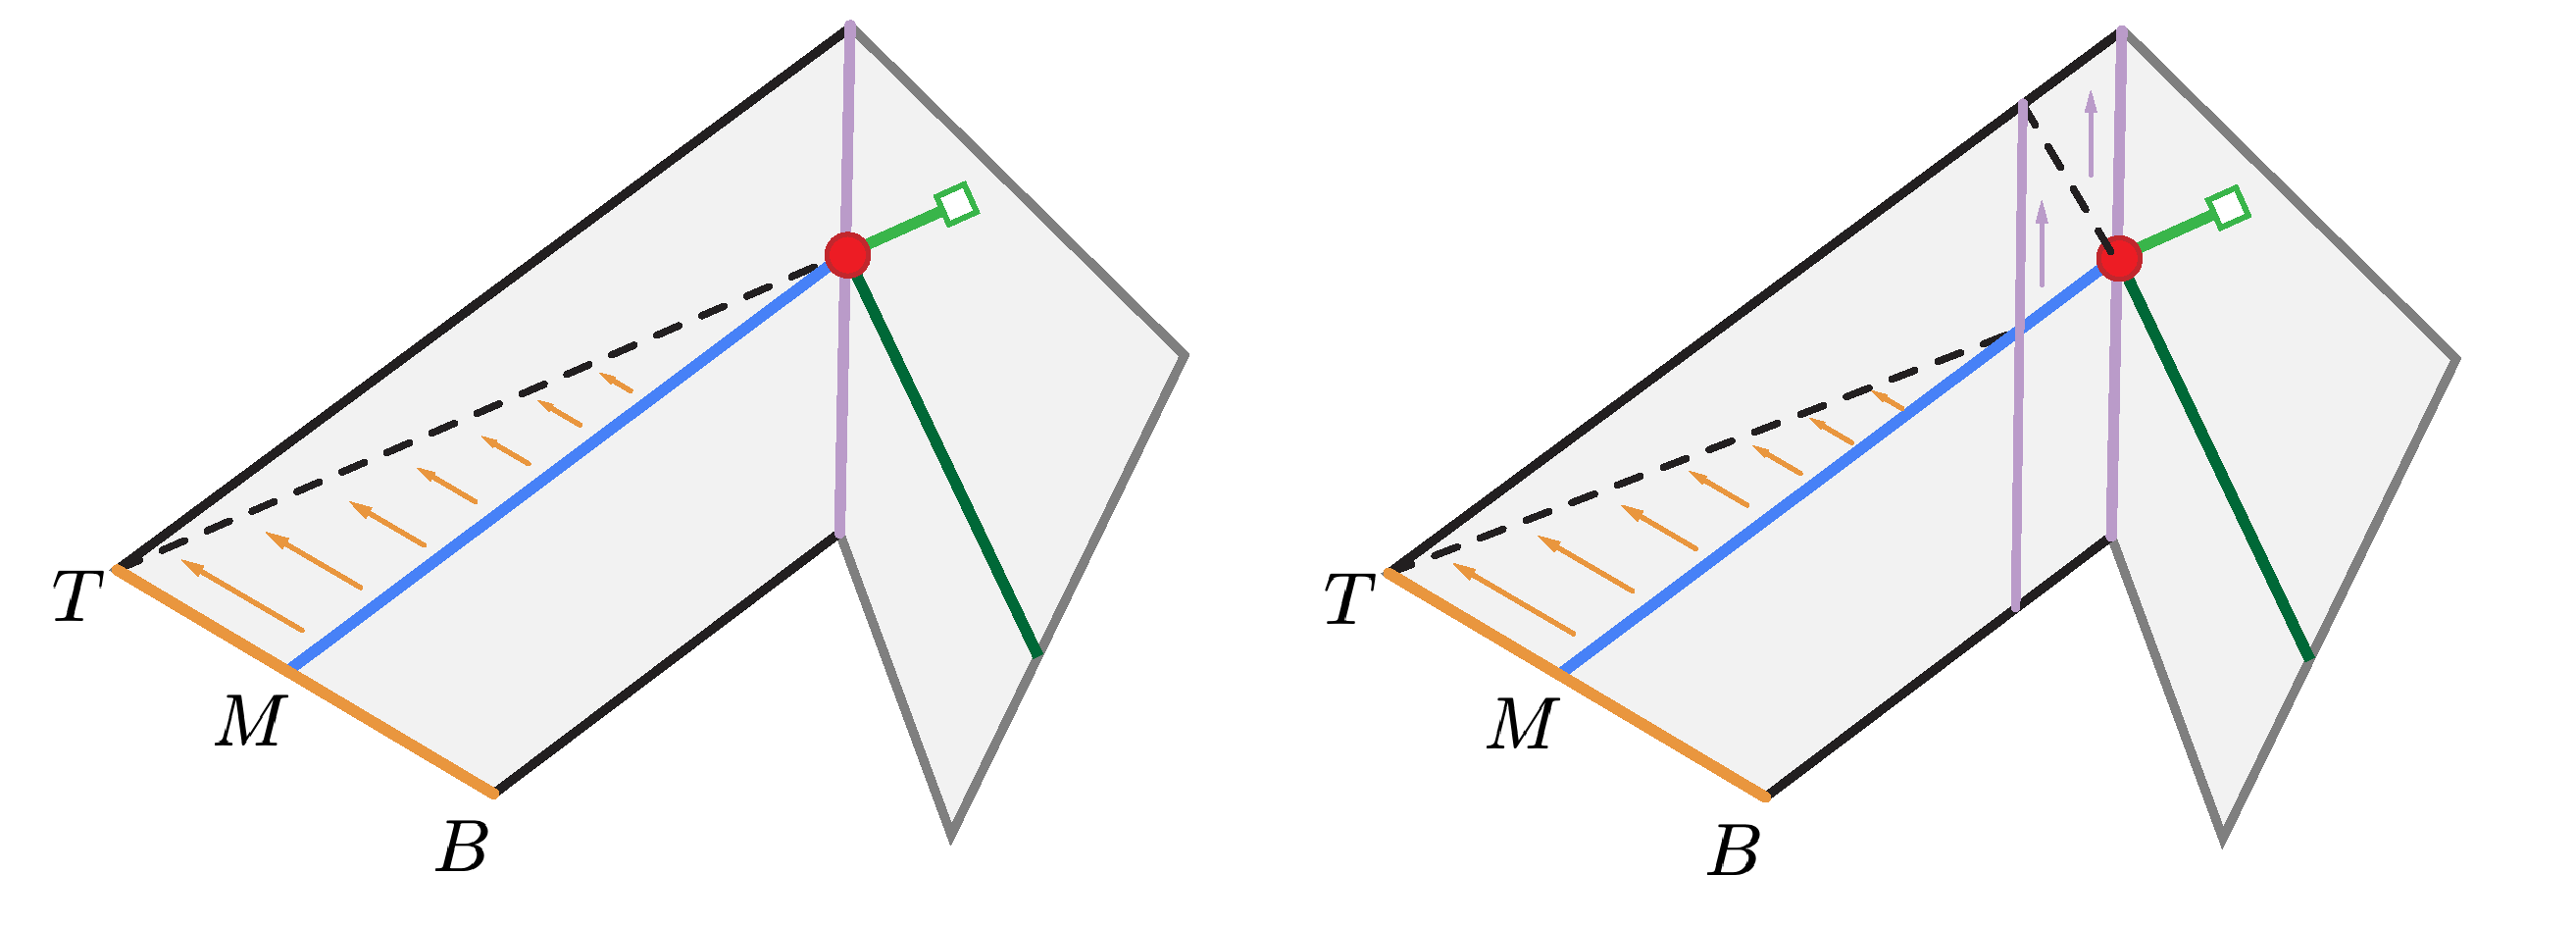
\includegraphics[width=0.9\linewidth]{prism-tex/figs/need_to_bevel}
    \caption{The vector field aligned with the pillar edge (orange) has a negative dot product with the green triangle normal; the tetrahedron with this field direction meets the green triangle at the red vertex. As a consequence, the mid-surface is not a section.
    After topological beveling, the shell becomes valid since the dot product between the green normal and the new pillar (purple) is positive.
    }
    \label{prism:fig:closed}
    
\end{figure}

Depending on the dihedral angles in the mesh $\T$,
it is possible that the dot product between one of the pillars (orange in Figure~\ref{prism:fig:closed}) and the face normals of some of the triangles from 1-ring neighborhood (green in Figure~\ref{prism:fig:closed}) is negative. 
While it may seem that this  problem could be addressed
by changing the definition so that each edge is assigned to one of the incident triangles, so that the field direction only in one incident tetrahedron needs to be considered, this problem is more significant than it may seem, as it leads to instability under small perturbations (e.g., due to floating-point rounding of coordinates). Such small perturbations can change the set of triangles intersecting a prism and thus violate the validity of the shell and, consequently, the bijectivity of $\P$.
We propose instead to refine $\T$, without changing its geometry, so that the shell corresponding to the refined mesh satisfies I2 (i.e., its middle surface is a section).
\paragraph{Topological Beveling.} We identify a prism $\Prism_v$ for which I2 does not hold and use a beveling pattern \cite{coxeter1973regular,conway2016symmetries,hart2018conway}
to decompose $\Prism_v$ in a way that $\T$ becomes a section for all 6 decompositions (I2). We refer to this operation as \emph{topological beveling}, as it does not change the geometry of the mesh, only its connectivity (Figure \ref{prism:fig:beveled_example}). 
We use the pattern in Figure \ref{prism:fig:patterns}a for $\Prism_v$, and we use the other two patterns (b) and (c) on the adjacent prisms to ensure valid mesh connectivity. The positions of the vertices are computed using barycentric coordinates (we used $t = 0.2$, i.e., the orange dot is at $1/5$ of the horizontal edge), and the normals of the newly inserted vertices are copied from the closest vertex (in Figure \ref{prism:fig:patterns}, the internal vertices have the normal of the triangle corner with the same color).

\begin{figure}
    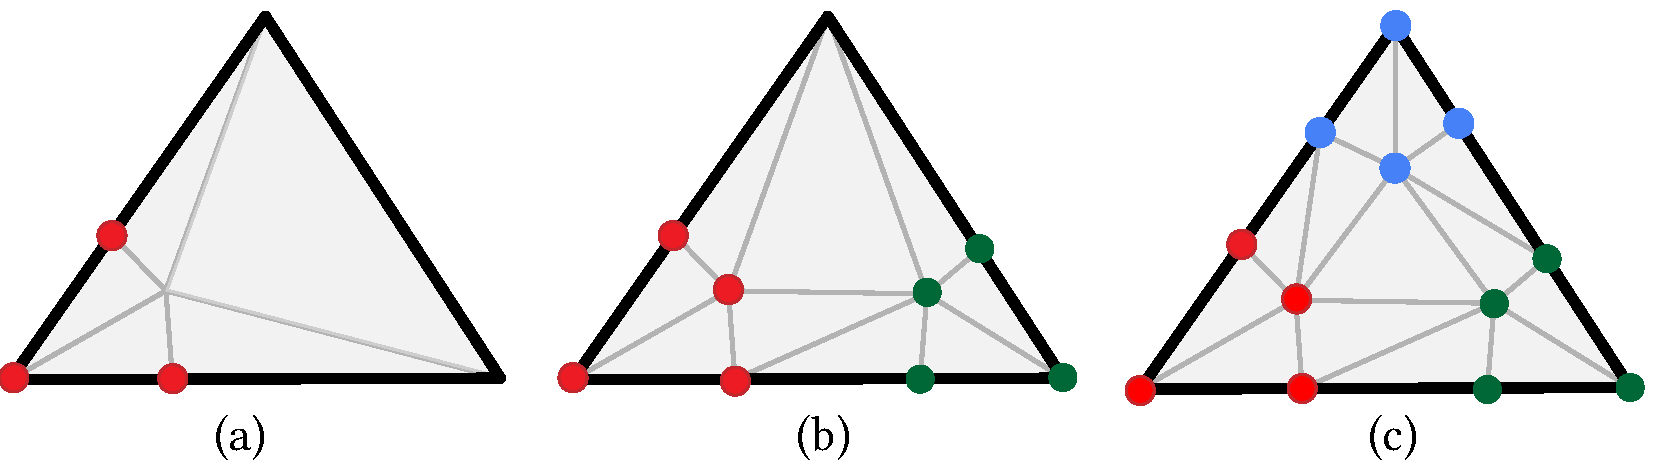
\includegraphics[width=0.9\linewidth]{prism-tex/figs/bevel}
    \caption{The beveling patterns used to decompose prisms for which $\T$ is not a section.}
    \label{prism:fig:patterns}
    
\end{figure}

\begin{figure}
    \includegraphics[width=\linewidth]{prism-tex/figs/screwdriver_bevel}
    \caption{Our algorithm refines the input model (left) with beveling patterns (middle) to ensure the generation of a valid shell. The subsequent shell optimizations gracefully remove the unnecessary vertices (right).}
    \label{prism:fig:beveled_example}
    
\end{figure}

\begin{theorem}
\label{thm:bevel}
Suppose $\T$ is the middle surface of $\S$, and neither $T_\S$ or $B_\S$ intersects with $\T$. After topological beveling, I2 holds, that is, $\T$ is a section of the shell $\S$ for all 6 decompositions.
\end{theorem}
\begin{proof}
    To show that $\T$ is a section of $\S$ we need to show that (1) $M_\Prism= \T \cap \Prism$ is a simply connected patch  for any prism of $\S$
and (2) for {each prism $\Prism$} and every point $p\in M_\Prism$ the dot product between the face normal $n(p)$ and the {pillars} $\V_i, i=1,2,3$ is strictly {positive}.

(1) is trivial since for every prism $\Prism$ of $\S$, $\Prism$ contains exactly one {triangle of the topological bevel refinement} face of $\T$.% (eventually subdivided by the beveling pattern without changing its geometry).


To prove (2), consider the dot products of the normals of each of the triangles in the beveled region sharing at least a vertex with $M_\Prism$, and the vectors along the pillars of $M_\Prism$.
We use colors to refer to the triangles of beveled prisms as shown in Figure~\ref{prism:fig:bevel-explain} left. 


\begin{figure}
    \centering
    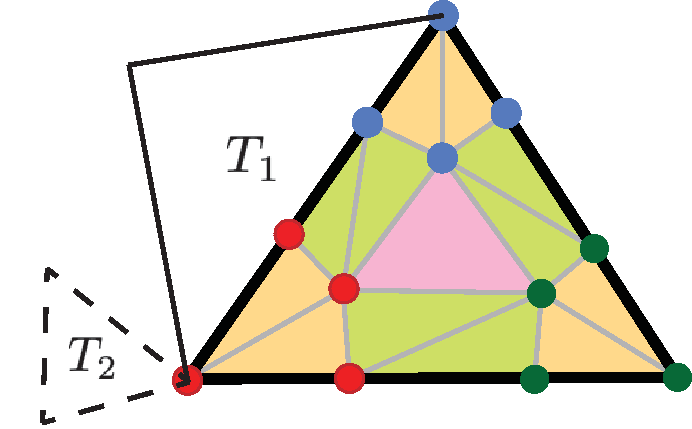
\includegraphics[width=0.5\linewidth]{prism-tex/figs/bevel_colors}
    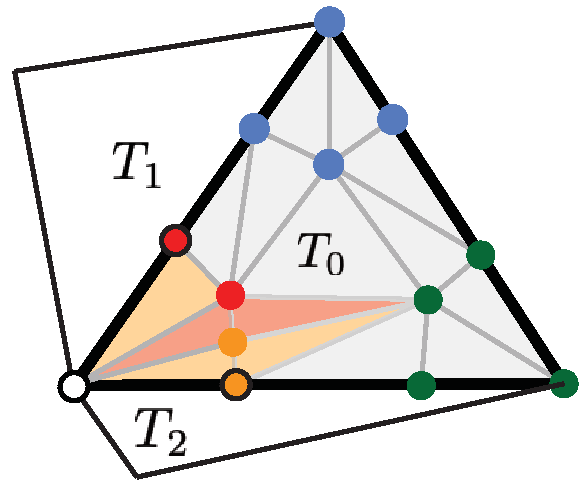
\includegraphics[width=0.4\linewidth]{prism-tex/figs/singularity-bevel-explained}
    \caption{Bevel patterns used in the proofs in Appendix~\ref{app:bevel} and Section~\ref{sec:extend-singularity}}
    
    \label{prism:fig:bevel-explain}
    \vspace{-1em}
\end{figure}
% The prism on the pink... \DZ{incomplete sentence}
The prism {corresponding to} the {pink} triangle covers only the interior of the original triangle. It satisfies {the dot product condition} since {its pillars are copied from the solution of Problem~(\ref{eq:QP})} at each vertex. 
A similar argument can be made for the green {prisms}: each  {prism} 
{gets its pillars from the edges}
incident at two of the vertices, {which are compatible with the normal of the adjacent triangle (e.g., red and blue pillars have positive dot product with  {the normal of} $T_1$).}
Finally, the prisms corresponding to orange triangles cover the same one ring that was used to compute the {original pillars (e.g., red pillar is compatible with $T_1$ and $T_2$)}. Since the same {pillar} is used for  each of the 3 vertices of the original prism, {the dot product} is {unchanged}.

\end{proof}


\paragraph{Output}
The output of this stage is a valid shell with respect to $\T$ (Section \ref{prism:sec:strong}), that is, it satisfies I1 and I2.


\subsection{Shell Optimization}
\label{prism:sec:optimization}

During shell optimization, we perform local operations
(Figure \ref{prism:fig:local_operations})
on a valid shell to reduce its complexity and increase the quality. Before applying every operation, we check the validity of the operation to ensure that: (1) the resulting middle surface will be manifold \cite{dey1999topology} and (2) the shell will be valid with respect to $\T$ (to ensure a bijective projection). We forbid any operation that does not pass these checks.  
{We would like to remark that, 
while there are different choices to guide the shell modification, we
experimentally discovered that allowing shell simplification and optimization consistently leads to thicker shells with a richer space of sections.} 

\begin{theorem}\label{thm:invariants}
Let $\S$ be a valid shell with respect to a mesh $\T$ and let $C=\{\Prism_i\}_{i\in I} \subset \S$ be a collection of prisms such that the middle surface $M_C$ of $C$ is a simply connected topological disk.

Let $\mathbb{O}$ be an operation replacing $C$ with a new collection of prisms $C'=\{\Prism_i'\}_{i\in I'}$, preserving both geometry and connectivity of the sides of the prism collection $C$, and ensuring that $M_{C'}$ is a simply connected topological disk.

If these three assumptions hold:
\begin{enumerate}
    \item property I1 holds for $C'$, %1
    \item the top and bottom surfaces of $C'$ do not intersect $\T$ ($T_{C'} \cap \T = B_{C'}\cap \T = \varnothing$), %4
    \item the dot product condition $n(p) \cdot \V(p)>0$ is satisfied for all points $p \in \T\cap \Prism_i'$ for all pillars of every prism $\Prism_i'$ of $C'$, %5
\end{enumerate}
then, $\forall i \in I'$, $\T \cap \Prism_i'$ is a simply connected topological disk.
In other words, $\T$ is a section of the new shell $\S'$ obtained by applying the operation  $\mathbb{O}$ to $\S$.
\end{theorem}
\begin{proof}

    We use $A^\circ$ to denote the interior of a set $A$. 
    We first assert that the topological disk patch $\T \cap C$ coincides with $\T \cap C'$.
    To make the notation more concise, we define $\T_C = \T \cap C$ and $\T_{C'} = \T \cap C'$.
    
    We show that $\T_C \subset C'$ by contradiction: assume there is $p\in \T_C$ but $p \not\in C'$.
    Choose a point $q \in \partial \T_C$,  that belongs to single prisms in $C$ and $C'$ and denote the enclosing prism in $C$ as $\Prism_q$ and the corresponding one in $C'$ as $\Prism_{q}'$.
    It follows from the positivity of the volumes of $\Prism_q$ and $\Prism_q'$ (Assumption 1), that there is  $\varepsilon>0$ such that the half-ball (for sufficiently small $\varepsilon$)  $\text{Ball}(q, \varepsilon) \cap \Prism_q$  coincides with $ \text{Ball}(q, \varepsilon) \cap \Prism_q'$.
    Futhermore, the validity of the initial shell guarantees that there exists an interior point $\bar{q} \in \text{Ball}(q, \varepsilon) \cap \Prism_q^\circ \cap \T$, and $\bar{q}\in \Prism_q'^\circ \cap \T \subset C'^\circ\cap \T$.
    
     Since neither $p$ or $\bar{q}$ lies on the boundary side triangles of $\partial C'$ (since $p,\bar{q}\notin\partial \T_C$), therefore there exists an interior path $P$ (i.e., a path both in $\T_C$ and in $\T_{C'}$) that connects $p$ and $\bar{q}$. By continuity the path $P$ it will cross $\partial C'$ at some point $p_i\in \T_C$. 
    Since the $\partial \T_{C'} = \partial \T_C$ is a fixed boundary loop (by the definition of $\mathbb{O}$), and does not contain interior points, $p_i$ can only cross on the top surface or bottom surface of $C'$ which contradicts Assumption 2. The roles of $C$ and $C'$ can be inverted to complete the proof. 
    
    We then  map $M_C$ to a
    regular planar $n$-gon $D$, with vertices on $\partial M_C$ mapped cyclically to the vertices of $\partial D$.
    It follows from \cite[Corollary 6.2]{floater2003one} that such a convex combination mapping $\varphi\colon M_C \to D$ is bijective. Then, similarly to the construction in Theorem~\ref{thm:projection},
    we 
    %``lift'' $D$ and 
    define $\phi\colon C \to D\times[-1,1]$ through affine mapping induced by the thetrahedralization of the prisms $\Prism_i$.
    %
    Similarly, we define $\psi \colon C' \to D\times[-1,1]$. The mapping $\psi$ is also bijective because of Assumption 1 and the definition of $\mathbb{O}$ it follows that the codomain of $\psi$ is the same as $\phi$.
    %
    Note that in both cases, the map transforms the vector field $\V(p)$ to the constant vector field $e_z = (0,0,2)$, and the projection is $\P_z$, as defined in the proof of Theorem~\ref{thm:projection}. 
    
    The dot product condition (Assumption 3) ensures that $\P_z$ defines a bijection between $D$ and $\psi(\T_C)${;} and further, the image {satisfies} $\P_z(\psi(\Prism_i'\cap \T)) = \psi(M_i')$ where $M_i'$ is the middle surface (a single triangle) of $\Prism_i'$.
    Therefore, since $\psi$ and $\P_z$ are both continuous and bijective, they are homeomorphisms which preserve topology, 
    thus $\Prism_i'\cap \T $ is a simply connected topological disk.
\end{proof}


We note that assumption (2) in Theorem~\ref{thm:invariants} prevents the input surface from crossing the bottom/top surface, thus avoiding it to move in the interior of a region covered by more than one prism. 

Our local operations (satisfying the definition of $\mathbb{O}$ in Theorem \ref{thm:invariants}) are translated from surface remeshing methods \cite{dunyach2013adaptive} since our shell can be regarded as a triangle mesh (middle surface) extruded through a displacement field $\N$. All the local operations described below directly change the middle surface, and consequently affect the extruded shell. After every operation, the middle surface is recomputed by intersecting $\T$ with the edges of the prisms in $\S$.
%\DZ{This is not clear,expand}
\begin{figure}
    \centering
    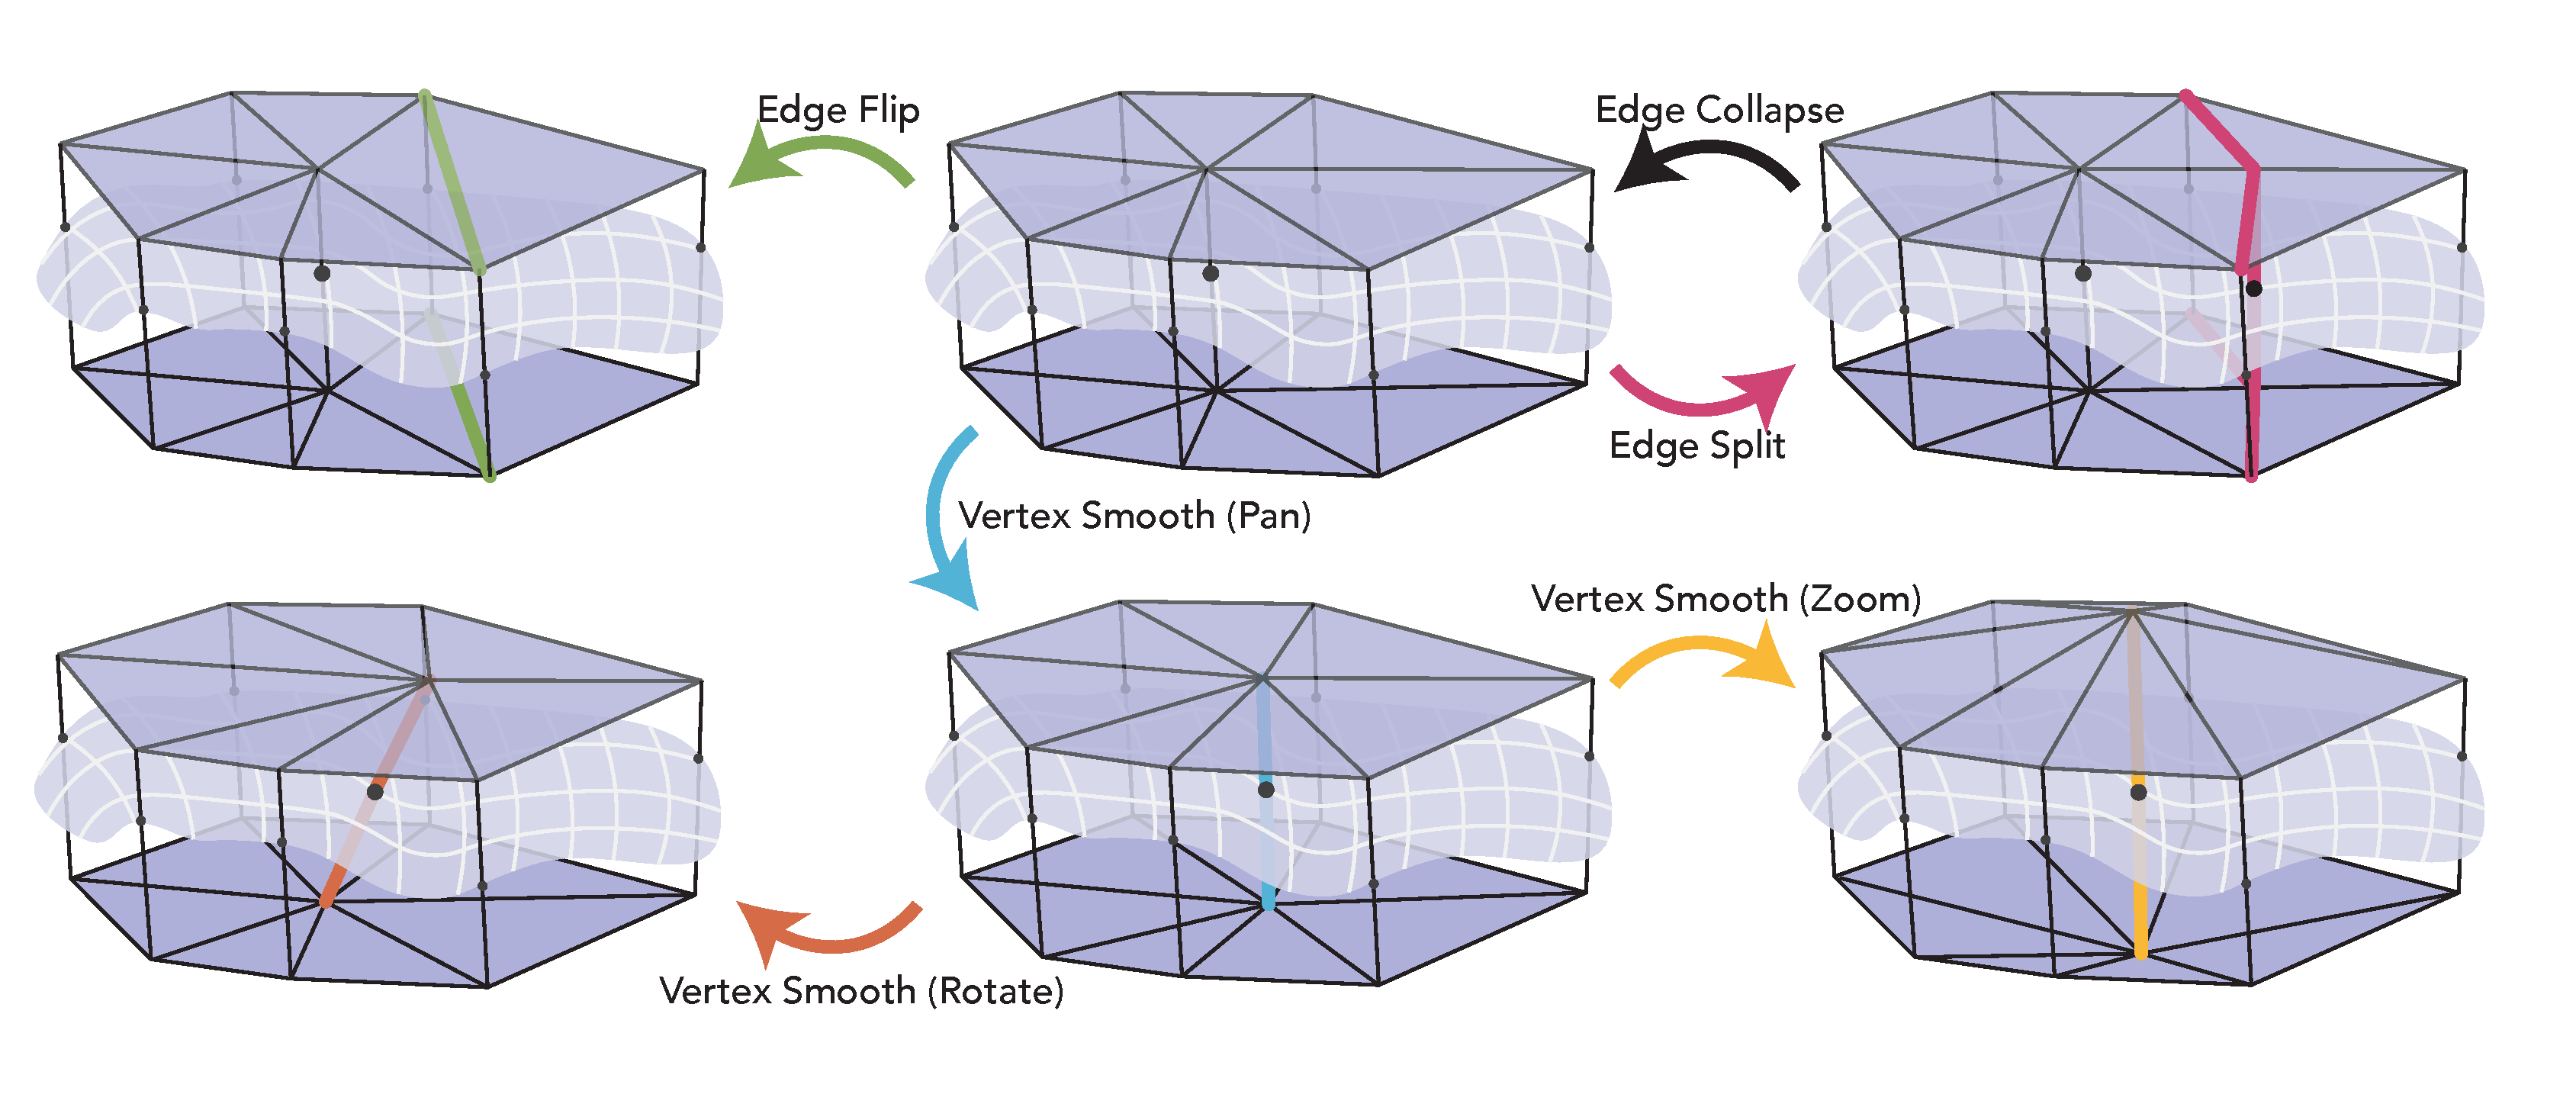
\includegraphics[width=0.9\linewidth]{prism-tex/figs/local-operations}
    % \includegraphics[0.5\linewidth]{prism-tex/figs/block_singular}
    \caption{Different local operations used to optimize the shell. Mesh editing operations translate naturally to the shell setting. For vertex smoothing, we decompose the operation into 3 intermediate steps: pan, zoom, and rotate.}
    \label{prism:fig:local_operations}
    
\end{figure}

\paragraph{Shell Quality}
We measure the quality of the shell $\S$ using the MIPS energy \cite{hormann2000mips} of its middle surface $M_\S$. For each triangle $T$ of the middle surface, we build a local reference frame, and  compute the affine map $\J_T$ transforming the triangle into an equilateral reference triangle in the same reference frame. The energy is then measured by
\begin{equation*}
    \sum_{T \in M_\S} \frac{\tr(\J_T^T\J_T)}{\det(\J_T)}.
\end{equation*}
This energy is invariant to scaling, thus allowing the local operations to coarsen the shell whenever possible while  encouraging the optimization to create well-shaped triangles. Good quality of the middle surface decreases the chances, for the subsequent operations, to violate the shell invariants.

\paragraph{Shell Connectivity Modifications.} We translate three operations for triangular meshes to the shell settings (Figure~\ref{prism:fig:local_operations} top). Edge collapse, split, and flip operations can be performed by simultaneously modifying the top and bottom surfaces
and retrieve the positions for the middle surface through the intersection. We only accept the operations if they pass the invariant check.

\paragraph{Vertex Smoothing.} Due to the additional degree of freedom on vertex-pairs (position, direction, and thickness), we decompose the smoothing operations into three {components} (Figure~\ref{prism:fig:local_operations} bottom). 
\emph{Pan} moves the positions of the top and bottom vertex at the same time, 
minimizing the MIPS quality of the middle surface. Neither the thickness or direction will be changed. 
\emph{Rotate} re-aligns the local direction to be the average of the neighboring ones while keeping the position of the middle vertex fixed. 
\emph{Zoom} keeps the direction and position of the middle vertex, and set the thickness of both top and bottom to be 1.5 times of the neighbor average, capped by the input target thickness.


\paragraph{Invariant Check}
% Our algorithm maintains both invariants using exact predicates \cite{shewchuk1997adaptive}. 
We use exact orientation predicates \cite{shewchuk1997adaptive} to make sure all the prisms satisfy positivity (I1). Further, we ensure that the original surface $\T$ is not intersecting with the bottom and top surface, except at the prescribed singularities.
The check is done using the triangle-triangle overlap test \cite{guigue2003fast}, accelerated using a static axis-aligned bounding box tree constructed from $\T$. 
To accelerate the checks for normal condition, 
for each prism $\Prism_i$, 
we maintain a list triangles overlapping with its convex hull (an octahedron), 
and check their respective normals against all the three pillars of $\Prism_i$. These three checks ensure that the three conditions in  Theorem~\ref{thm:invariants} are satisfied.
%
Note that the vertex smoothing operation is continuous, in the sense that any point between the current position and the optimal one improves the shell. 
We, however, handle it as a discrete operation to check our conditions: we attempt a full step, and if I1 is not satisfied, we perform a bisection search for a displacement that does. We avoid bisection for the other two conditions since they are expensive to evaluate.



\paragraph{Projection Distortion} 
An optional invariant to maintain (not {necessary} for guaranteeing bijectivity, but useful for applications), 
is a bound  on the maximal distortion $\D_\P(\Prism) $ of $\P$ for a prism $\Prism$. 
We measure it as  the maximal angle between the normals of the set $\C$ containing the faces of $\T$ intersecting $\Prism$ and $\V$:
\begin{equation*}
    \D_\P(\Prism) = \max_{p \in \C} \angle (n_p, \V(p)),
\end{equation*}
where $\angle$ is the unsigned angle in degrees. This quantity is bounded from below by the smallest dihedral angle of $\T$, making it impossible to control exactly. However, we can prevent it from increasing by measuring it and discarding the operations that increase it. In our experiments, we use a threshold of $89.95$ degrees.

\paragraph{Scheduling and Termination}
Our optimization algorithm is composed of two nested loops. The outer loop repeats a set of local operations until the face count between two successive iteration decreases by less than 0.01\%. In the inner loop we: (1) flip every edge of $\S$ decreasing  the MIPS energy and avoiding high and low vertex valences \cite{dunyach2013adaptive}; (2) smooth all vertices which include pan, zoom, and rotate; and (3) collapse every edge of $\S$ not increasing the MIPS energy over {30}. Note that for every operation, we check the invariants, the projection distortion, and manifold preservation and reject any operation violating them.
%
After the outer iteration terminates (i.e.  the shell cannot be coarsened anymore), we further optimize the shell with 20 additional iterations of flips and vertex smoothing.




% \TS{new text done with Zhongshi, old text is on the bottom, probably kill it}

% We separate the operations into \emph{outer passes, which contains only one of the operations (either collapse, flip or smooth), and}
% iteratively perform \emph{outer passes} composed of one sequence of edge collapse, one of edge flip, and one of vertex smoothing. We stop these iterations when the face count between different passes decreases by less than 0.01\%. We then further optimize the shell with 20 additional passes of flips and vertex smoothing.

\begin{figure}
    \centering
    \includegraphics[width=\linewidth,draft=false]{prism-tex/figs/doublewheel_pinch}
    % \includegraphics[0.5\linewidth]{prism-tex/figs/block_singular}
    \caption{A model with 48 singularities and a close up around one (left).
    Our shell is pinched around each of them without affecting other regions (right).}
    \label{prism:fig:singularity_example}
    
\end{figure}


\subsection{Singularities}\label{prism:sec:singularities}

% We introduced the algorithm assuming that problem \eqref{eq:OPT} always has a solution, and assuming that our mesh does not contains boundaries. We will now extend our construction to handle these cases, which requires minor variations to our algorithm.

Singularities, i.e. vertices of $\T$ for which the constraints set of problem \eqref{eq:OPT} is empty, are surprisingly common in large datasets (Figure~\ref{prism:fig:singularity_example} shows an example). For instance, in our subset of Thingi10k \cite{zhou2016thingi10k}, although only 0.01\% vertices are singular,  8\% of the models have at least one singular point. This has been recently observed as a limitation for the construction of nested cages \cite[Appendix A]{sacht2015nested}, and it is a well-known issue when building boundary layers \cite{aubry2015most,aubry2017boundary,garimella2000boundary}.
%
There are two main situations that give rise to singular points. 
The first one naturally generates a singular point when more than two ridge-lines meet (e.g., figures~\ref{prism:fig:singularity_example} and~\ref{prism:fig:singularity-boolean}), thus making the point a feature point. 
The second one is a pocket-like mesh artifact, often produced as a result of mesh simplification (Figure~\ref{prism:fig:singularity-illustration}).

While singularities might seem fixable by applying local smoothing or subdivision as a pre-process, it is not desirable in the case of a feature point, and is likely to introduce self-intersection or more serious geometric inconsistency.
%in the presence of the meshing artifacts.
Therefore, due to the above reasons and observing that they are very uncommon, we propose to extend our theory (Section~\ref{sec:extend-singularity}) and algorithm to handle isolated singularities  by \emph{pinching} the thickness of the shell. Note that in the rare case where two singular points are sharing the same edge, they are \emph{automatically} separated by our topological beveling.

\paragraph{Pinching.} 
We extend our definition of the shell by allowing it to have zero thickness on singularities, thus tessellating the degenerate prism with 4 instead of 6 tetrahedra (Figure~\ref{prism:fig:singularity-illustration}). We further remark that these isolated points must be excluded from Definition~\ref{def:section}. In the implementation, this requires to change the intersection predicates to skip the singular vertices.
With this change, the singularity becomes a trivial point of the projection operator $\P$,
% \DZ{all middle surface points are fixed points of $\P$}
and the rest of our shell can still be used in applications without further changes. Since singularities tends to be isolated (they are usually located at the juncture of multiple sharp features), this solution has minimal effects on applications: for example, when our shell is used for remeshing, pinching the shell at singularities will freeze the corresponding isolated vertices while allowing the rest of the mesh to be freely optimized.

\begin{wrapfigure}{r}{0.3\linewidth}
    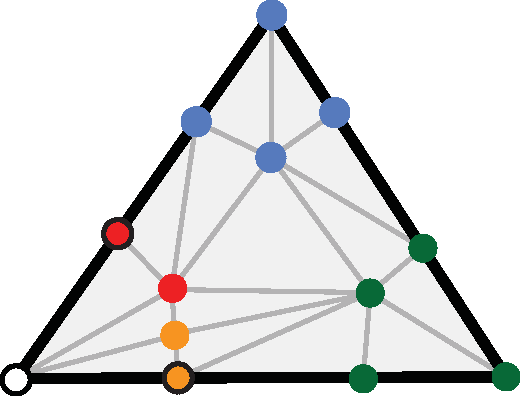
\includegraphics[width=1\linewidth]{prism-tex/figs/singular_bevel}
\end{wrapfigure}

\begin{figure}
\centering
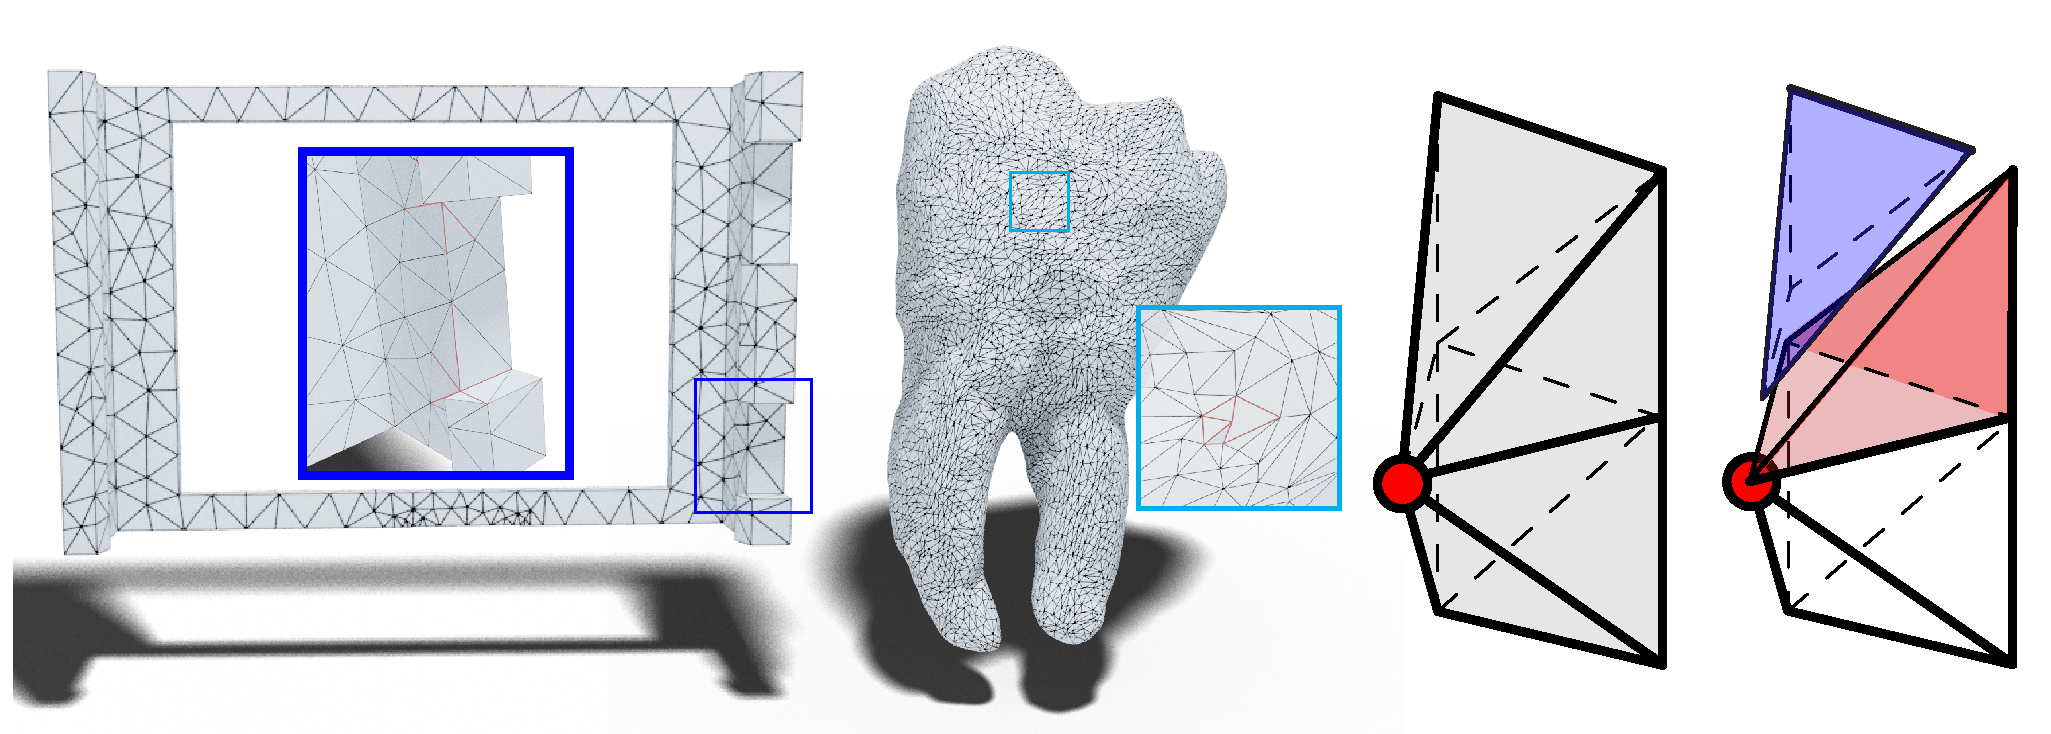
\includegraphics[width=\linewidth]{prism-tex/figs/degenerate_prism_decompose}
\caption{Left to right: examples of a singularity as a feature point and as a meshing artefact; and illustration of the degenerate prism with a singularity (red) and its tetrahedral decomposition made of only four tetrahedra.}
\label{prism:fig:singularity-illustration}

\end{figure}

The topological beveling algorithm is changed most significantly: for singularities, there is no pillar to copy from.
In this case, we apply an additional edge split, to use the pattern in the inset (with the singularity marked by a white dot) in the one-ring neighborhood of the singularity.
The newly inserted vertices lie either inside a triangle (uncircled red and orange dots), 
or in the interior of an edge (circled red and orange dots).
Therefore, we assign to the orange vertices the average normal of the two adjacent triangles, and to red the pillar of the connected orange one.


Additionally, the edges connecting singularities will always be beveled/split after beveling. Therefore no prism will contain more than one singular point.
We discuss the technical extensions for our proofs to shells with pinched prisms as follows,

\subsection{Extension to meshes with Singularities}\label{sec:extend-singularity}
Most of the proofs and definition in Section~\ref{prism:sec:method} easily extends to meshes with singularity or pinched shells. For instance,
{both} Theorem~\ref{thm:projection} and Definition~\ref{def:validshell} apply to pinched shells by just considering a prism made of 4 (2 for the top and 2 for the bottom slab) instead of 6. Propositions~\ref{thm:I1} and~\ref{thm:thickness} both rely on per-vertex properties; by just excluding singular vertices (and neighboring prism) from the statements the proofs (and our algorithm) still holds.


Theorem~\ref{thm:invariants} requires some minor additional considerations. As a consequence of beveling, no two singularities are adjacent. Therefore, we can always find a point $q \in \partial \T_C$ that belongs to a single prism (Appendix~\ref{app:invariant-checks}) since every prism will have a positive volume
because no singularities are adjacent.


Finally Proposition~\ref{thm:bevel} requires a new proof since the beveling pattern used for singularities is different.
% \begin{proposition}
% For a prism $\Prism$ with one singularity, 
% \end{proposition}
\begin{proof}
In  Figure~\ref{prism:fig:bevel-explain} right, we highlight in red and orange the triangles not covered by the discussion in Appendix~\ref{app:bevel}. 
The prism corresponding to an orange middle triangle intersects the edge-adjacent triangle. And since the new pillars are computed as the average of the normals of the two adjacent triangles with dihedral angle strictly less than $360^\circ$ 
 (Section~\ref{prism:sec:singularities} inset), each dot product is positive. 
The prism {for} a pink middle triangle intersects only the interior of the original triangle, and the dot product between the pillars and the triangle normal are positive by construction. 
\end{proof}



\begin{figure}
    \centering
    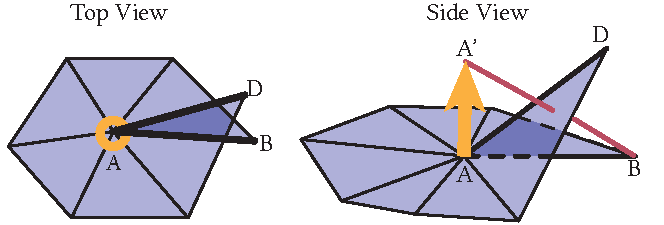
\includegraphics[width=0.9\linewidth]{prism-tex/figs/boundary_singular}
    \caption{$AA'$ is a direction with positive dot product with respect to all its neighboring faces. However, no valid shell can be built following that direction.}
    \label{prism:fig:boundary_singularity}
    
\end{figure}

\subsection{Boundaries.}\label{prism:sec:boundaries}

We introduced our algorithm, assuming that the input mesh does not have boundaries. We will now extend our construction to handle this case, which requires minor variations to our algorithm.

For some vertices on the boundary, it might be impossible to extrude a valid shell (Figure~\ref{prism:fig:boundary_singularity}), even if problem \eqref{eq:OPT} has a solution, as  Theorem~\ref{thm:thickness} does not apply in its original form. 
%
We identify such cases by connecting every edge in the 1-ring neighborhood of the boundary vertex
to the extruded point and check if they collide with the existing 1-ring triangles (e.g., the triangle $A'AB$ intersects the existing input triangle in Figure~\ref{prism:fig:boundary_singularity}). If it is the case, we consider this vertex as a singularity, and we pinch the shell. Note that this is an extremely rare case and, in our experiments, we detected it only for models where the loss of precision in the STL export introduces rounding noise on the boundary.% (and the problem goes away increasing precision). We could not identify any realistic case of this scenario in our model collection.

Once we pinch all boundary singularities, our construction extends naturally to the boundary. The only necessary modification is in the shell optimization (Section~\ref{prism:sec:optimization}), where we skip all operations acting on boundary vertices to maintain the bijectivity of the induced projection operator (Figure~\ref{prism:fig:open-hand}).
%
We thus freeze these vertices and never allow them to move or be affected by any other modification of the shell. Note that, in certain applications, it might also be useful to freeze additional non-boundary vertices to ensure that these remain on the middle surface during optimization (e.g., to exactly represent a corner of a CAD model).


\begin{figure}
    \centering
    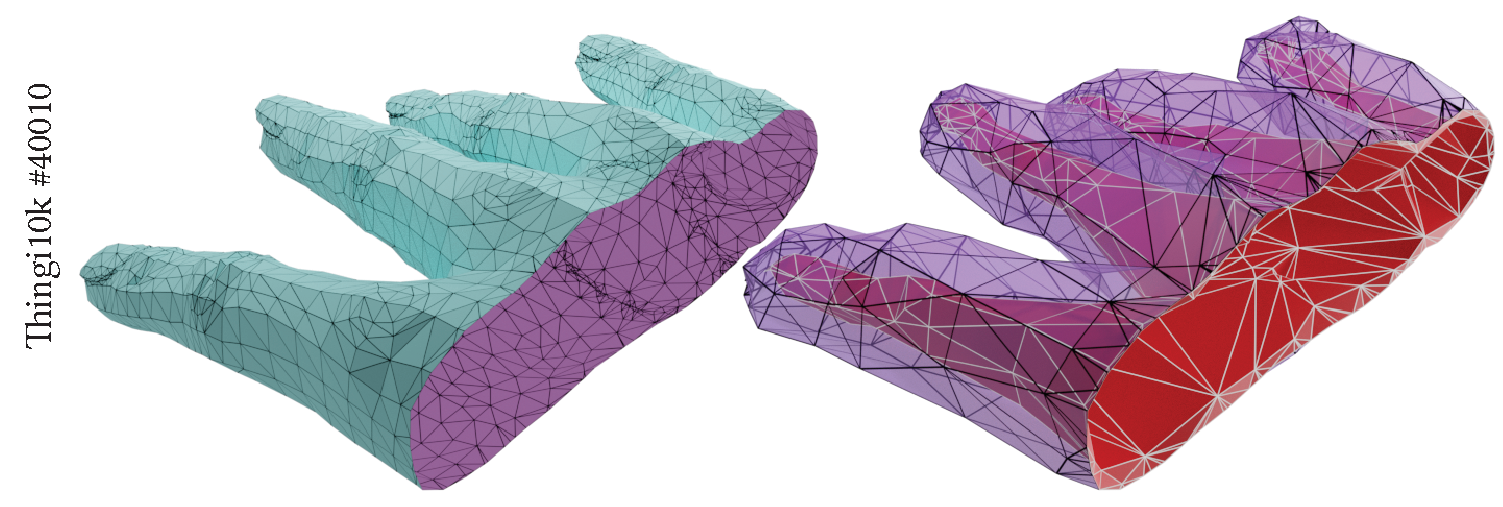
\includegraphics[width=0.9\linewidth]{prism-tex/figs/open-hand}
    \caption{An example of a mesh with boundary.}
    \label{prism:fig:open-hand}
    
\end{figure}




.
\section{Results}
\label{sec:results}
Our algorithm is implemented in C++ and uses Eigen \cite{eigenweb} for the linear algebra routines, CGAL \revision{\cite{cgal2008computational}} and Geogram \cite{levy2015geogram} for predicates and spatial searching, and libigl \cite{jacobson2016libigl} for basic geometry processing routines.
We run our experiments on cluster nodes with a Xeon E5-2690 v2 @ 3.00GHz.
The reference implementation used to generate the results is attached to the submission and will be released as an open-source project.

\paragraph{Robustness}

\begin{figure}
    \centering
    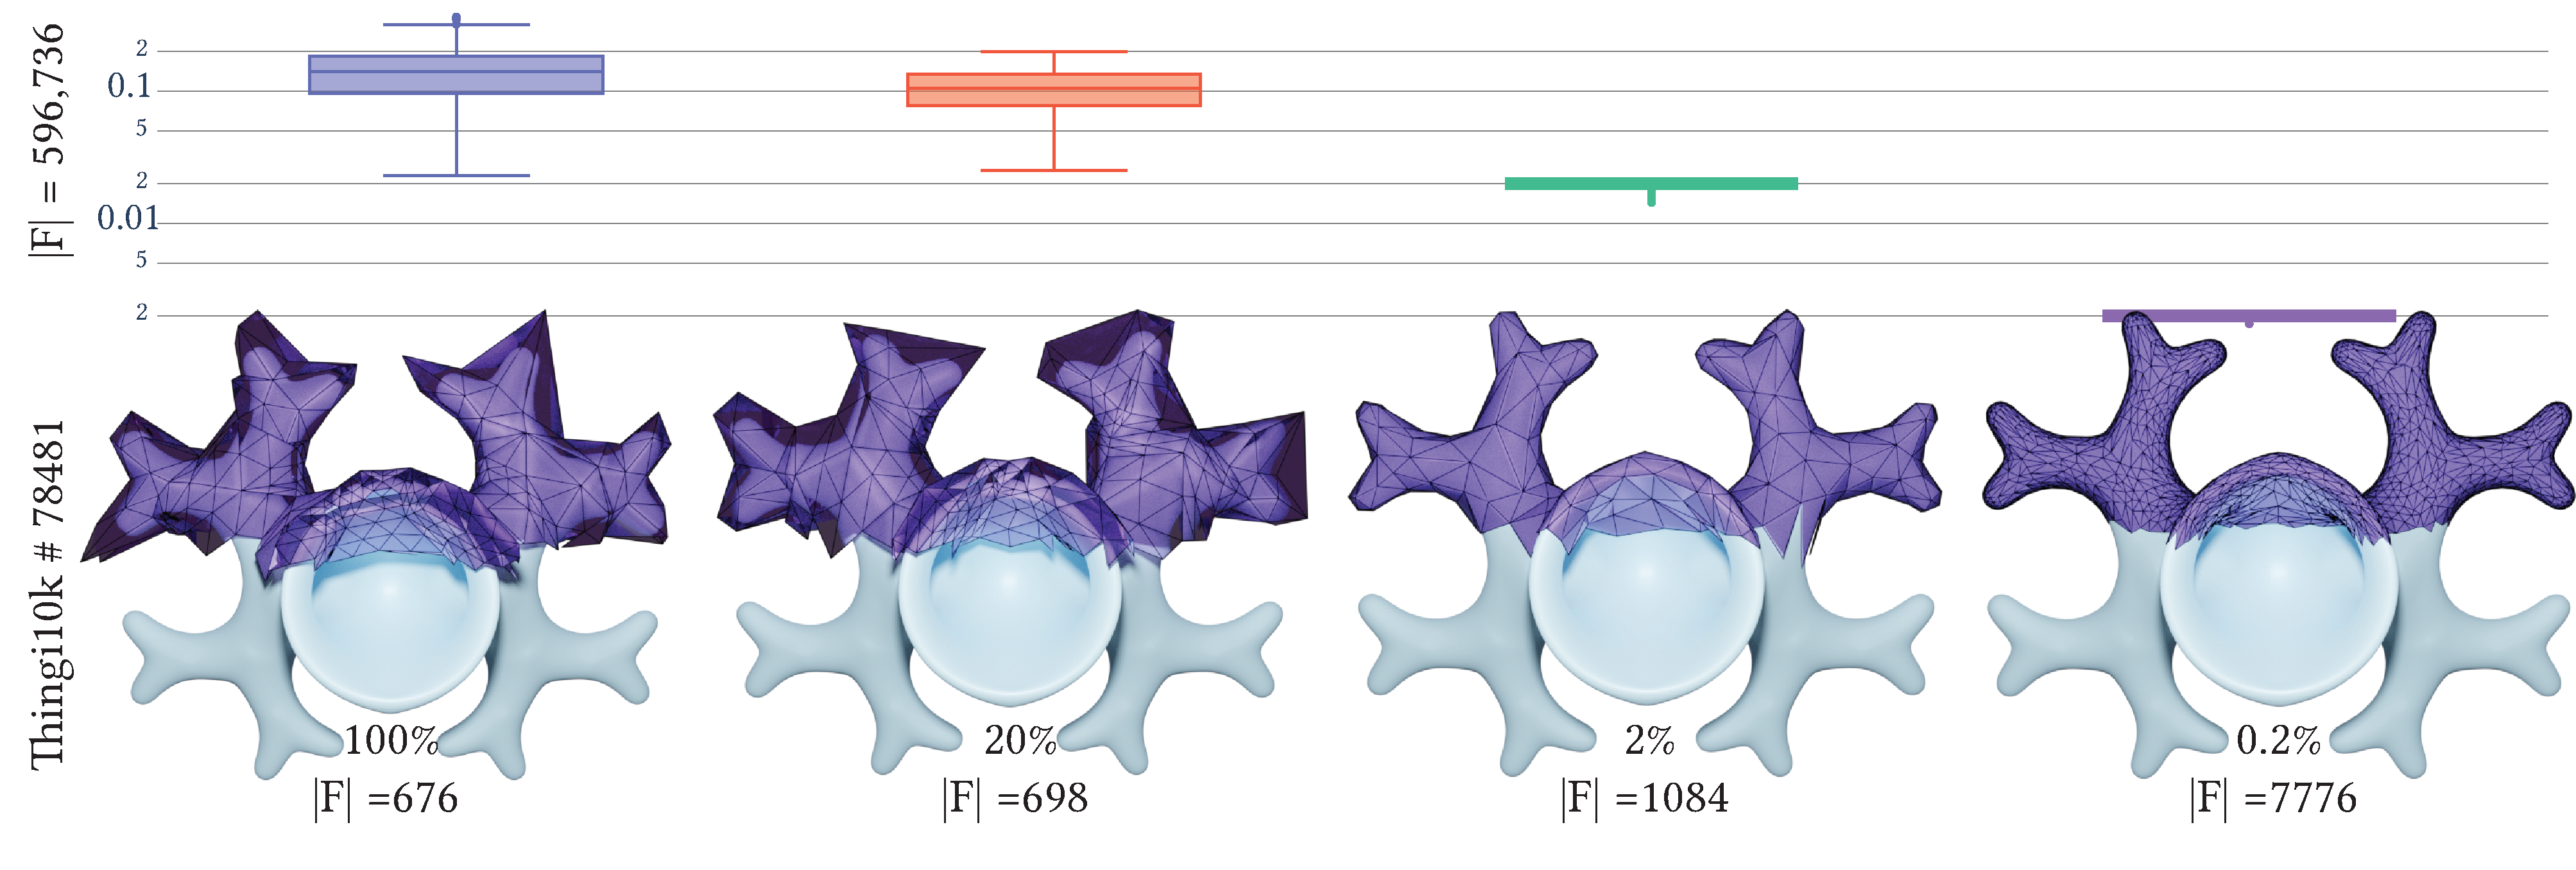
\includegraphics[width=\linewidth,draft=false]{prism-tex/figs/varying_thickness}
    %input F= 596736, Thingi10k 78481
    \caption{The effect of different target thickness on the number of prisms |F| of the final shell, 
    and distribution of final thickness (\revision{shown as the box plots on the} top).} 
    
    \label{prism:fig:vary_thick}
\end{figure}

For each dataset, we selected the subset of meshes satisfying our input assumptions:  intersection-free, orientable, manifold triangle meshes without zero area triangles (tested using a numerical tolerance $10^{-16}$).  We test self-intersections by two criteria: a ball of radius $10^{-10}$ around each vertex does not contain non-adjacent triangles; and all the dihedral angles are larger than 0.1 degrees.

We tested our algorithm on two datasets: (1) Thingi10k dataset \cite{zhou2016thingi10k} containing, after the filtering due to our input assumptions, 5018 models; and (2) the first chunk of for the ABC dataset~\cite{Koch_2019_CVPR} with 5545 models.
The only user-controlled parameter of our algorithm is the target thickness of our shell; in all our experiments (unless stated otherwise), we use 10\% of the longest edge of the bounding box. 
In Figure~\ref{prism:fig:vary_thick}, we show how the target thickness influences the usage of the shell: a thicker shell provides a larger class of sections, thus accommodates more processing algorithms, while a thinner one offers a natural bound on the geometric fidelity of the sections.

% We use a large thickness in our experiments to show that our algorithm can create it, even if we expect that a thinner shell will be more practical in most applications.

\begin{figure}
    \centering
    Thingi10k\\
    \includegraphics[width=0.9\linewidth]{prism-tex/figs/10k_gallery}\\%[0.5em]
    %
    ABC\\
    \includegraphics[width=\linewidth]{prism-tex/figs/abc_gallery}
    %
    \caption{Gallery of shells built around models from Thingi10k \protect\cite{zhou2016thingi10k} and ABC~\protect\cite{Koch_2019_CVPR}.}
    \label{prism:fig:gallery}
    
\end{figure}


Our algorithm successfully creates shells for all 5018 models for Thingi10k and 5545 for ABC. 
We show a few representative examples of challenging models for both datasets in Figure \ref{prism:fig:gallery}, including models with complicated geometric and topological details. In all cases, our algorithm produces coarse and thick cages, with a bijective projection field defined.

We report as a scatter plot the number of output faces, the timing, and the memory used by our algorithm (Figure \ref{prism:fig:large-dataset}).
In total, the number of prisms generated by our algorithm is 7\% and 2\% of the number of input triangles for the Thingi10k and ABC dataset respectively 
and runs with no more than 4.7 \revision{GB} of RAM. 
The generation and optimization of the shell takes 5min and 59s in average and up to 8.6 hours for the largest model. \revision{50\% of the meshes finish in 3 minutes and 75\% in 6 minutes and 15 seconds.}

% \begin{figure}
%     \centering
%     Thingi10k
%     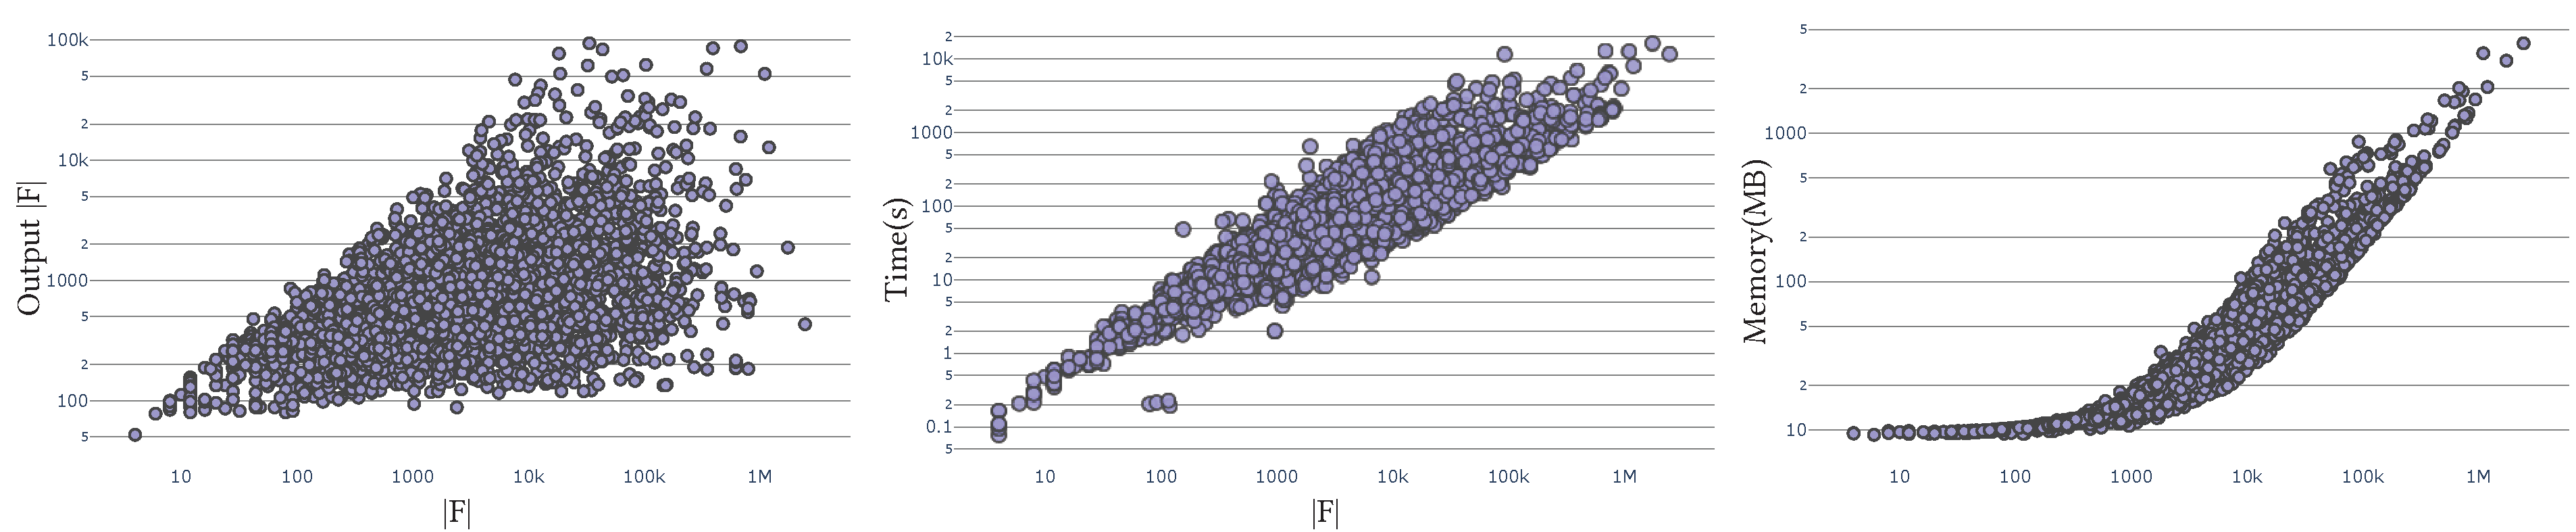
\includegraphics[width=\linewidth]{prism-tex/figs/stats10k}
%     ABC
%     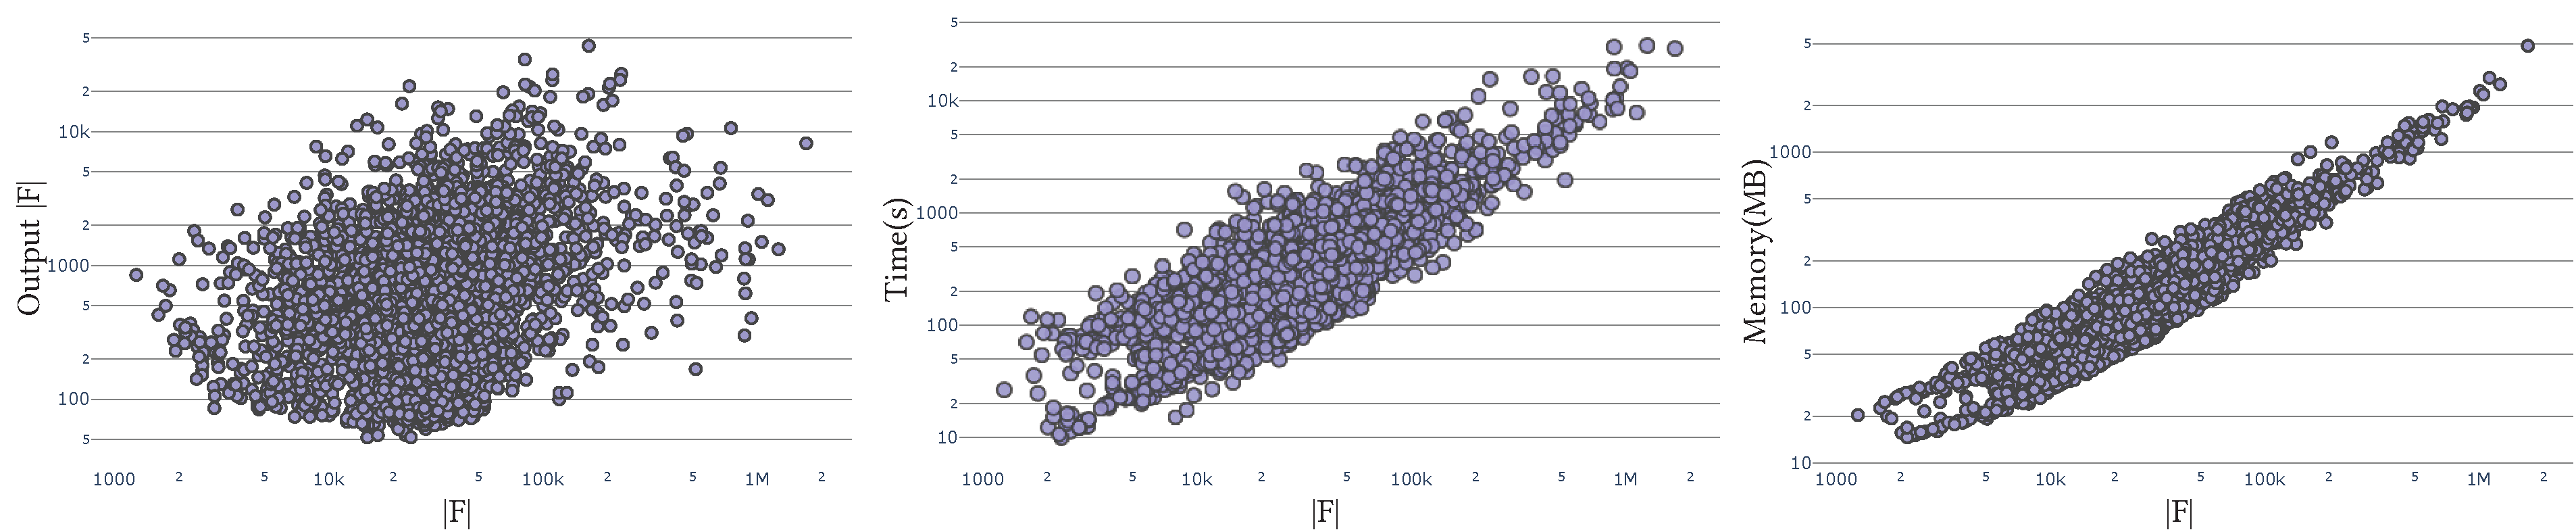
\includegraphics[width=\linewidth]{prism-tex/figs/stats_abc}
%     \caption{Statistics of 5018 shells in Thingi10k dataset \cite{zhou2016thingi10k} (top) and 5545 in ABC Dataset \cite{Koch_2019_CVPR} (bottom).}
%     \label{prism:fig:large-dataset}
%     
% \end{figure}
\begin{figure}
    \centering
    \begin{tabular}{cc}
        Thingi10k & ABC \\ 
        \includegraphics[width=0.4\linewidth,page=2]{prism-tex/figs/stats_combined}
        &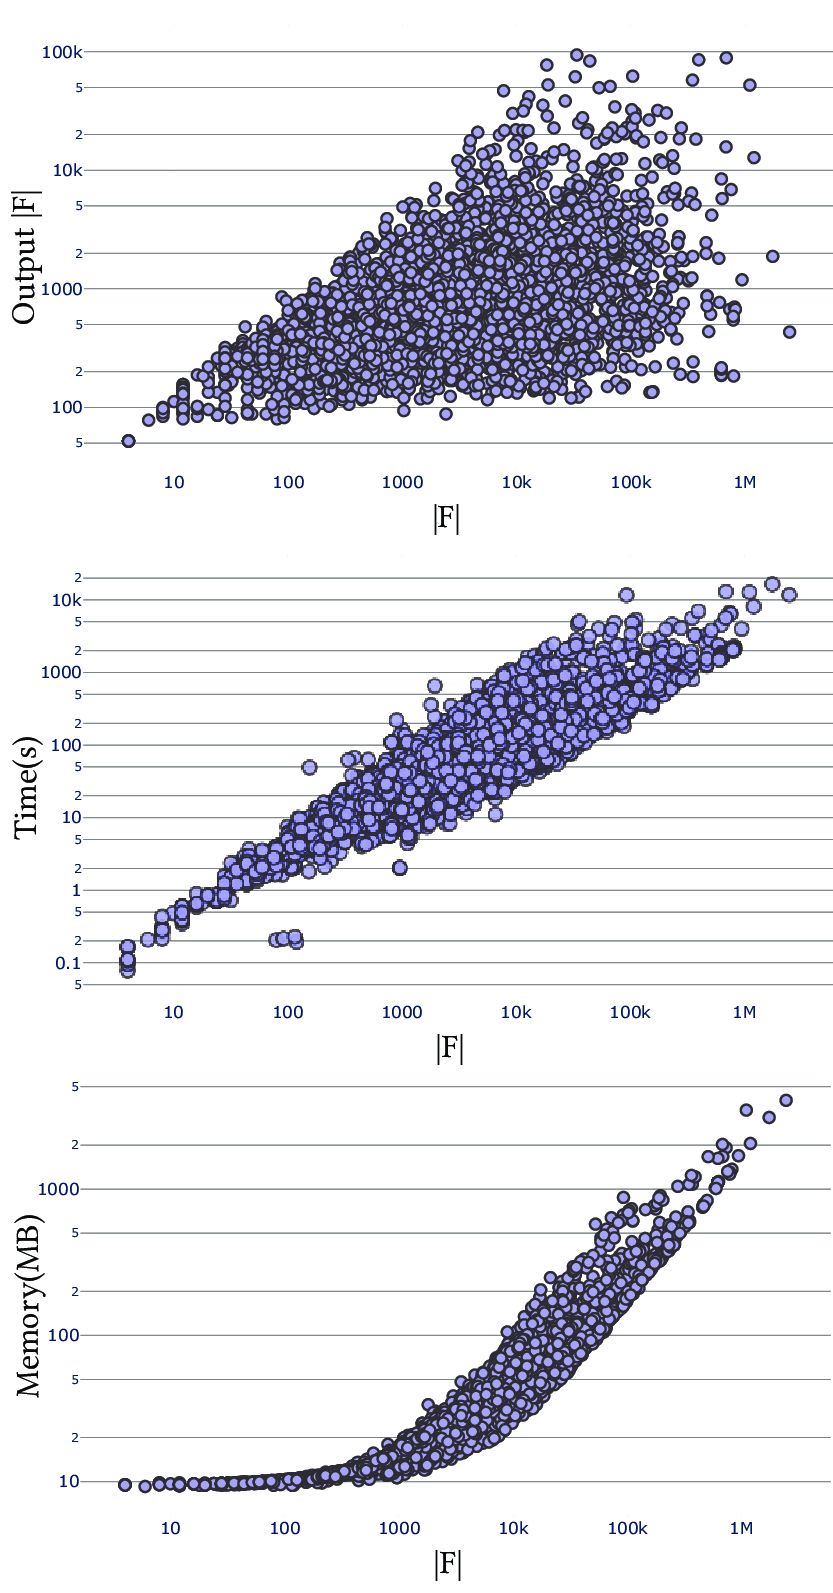
\includegraphics[width=0.4\linewidth,page=1]{prism-tex/figs/stats_combined}
    \end{tabular}
    \caption{Statistics of 5018 shells in Thingi10k dataset \cite{zhou2016thingi10k} (left) and 5545 in ABC Dataset \cite{Koch_2019_CVPR} (right).}
    \label{prism:fig:large-dataset}
    
\end{figure}


\begin{figure}
    \centering
    \includegraphics[width=1\linewidth]{prism-tex/figs/thai_comparision}
    \caption{The \emph{UV based method} cannot simplify the prescribed seams, and introduces self-intersections. 
    The projection induced by the \emph{Naive Cage} method is not continuous and not bijective; it leads to visible spikes in the reconstructed geometry.}
    \label{prism:fig:qslim_naive}
    
\end{figure}

\paragraph{Comparison to Simple Baselines}
In Figure~\ref{prism:fig:qslim_naive} we compare to two baseline methods based on \cite{garland1998simplifying}. For each method, we generate a coarse mesh, uniformly subdivide it for visualization purposes, 
%this is the old text % start with a uniformly subdivided coarse mesh, 
and query the corresponding spatial position on the original input to form the subdivided mesh.
% a mesh with subdivision connectivity. 
The \emph{UV based} method is a conventional way of establishing correspondence in the context of texture mapping. However, the robust generation of a UV atlas satisfying a variety of user constraints is still an open problem. We use the state-of-the-art methods \cite{li2018optcuts,jiang2017simplicial} to generate a low-distortion bijective parametrization, and use seam-aware decimation technique~\cite{liu2017seamless} to generate the coarse mesh.
Due to the complex geometry and the length of the seam (Figure~\ref{prism:fig:qslim_naive} second figure), the simplification is not able to proceed beyond the prescribed seam while maintaining the bijectivity, making the pipeline inadequate especially for building computational domains. 
%The reconstructed geometry also exhibits excessive distortion.

\revision{We also set up a baseline of the \emph{Naive Cage} method by creating} a simplified coarse mesh with \cite{garland1998simplifying} and use Phong projection to establish the correspondence \cite{kobbelt1998interactive,panozzo2013weighted}. \revision{Such attribute transfer} is not guaranteed to be bijective; some face may not be projected (Figure~\ref{prism:fig:qslim_naive} third image). With our method, we can generate a coarse mesh while having a low-distortion bijective projection (Figure~\ref{prism:fig:qslim_naive} fourth image).

\paragraph{Numerical accuracy} 
To evaluate the numerical error introduced by  our projection operator \revision{when implemented with floating-point arithmetic}, we \emph{transfer} the vertices of the input mesh to the middle surface and \emph{inverse transfer} them from the middle surface back to the input mesh.  We measure the Euclidean distance with respect to the source vertices (Figure~\ref{prism:fig:shark_accuracy}). 
We compare the same experiment with the Phong projection \cite{kobbelt1998interactive}. This alternative approach exhibits distance errors up to $10^{-5}$ even after ruling out the outliers for which the method fails due to its lack of bijectivity.  The maximal error of our projection is on the order of $10^{-8}$; this error could be completely eliminated (for applications requiring an exact bijection) by implementing the projection operator and its inverse using rational arithmetic.
\begin{figure}
    \centering
    \includegraphics[width=\linewidth]{prism-tex/figs/shark_accuracy}
    \caption{Our projection is three orders of magnitude more accurate than the baseline method, and bijectively reconstructs the input vertex coordinates.}
    \label{prism:fig:shark_accuracy}
    
\end{figure}
%%%%%%%%%%%%%%%%%%%%%%%%%%%%%%%%%%%%%%%%%%%%%%%%%%%%%
%%%%%%%%%%%%%%%%%%%%%%%%%%%%%%%%%%%%%%%%%%%%%%%%%%%%%
%%%%%%%%%%%%%%%%%%%%%%%%%%%%%%%%%%%%%%%%%%%%%%%%%%%%%
%%%%%%%%%%%%%%%%%%%%%%%%%%%%%%%%%%%%%%%%%%%%%%%%%%%%%
\section{Applications}
\label{sec:applications}
Using our shell $\S$, we implement the following predicates and functions:
\begin{itemize}
    \item $\isinside(p)$: returns true if the point $p \in \mathbb{R}^3$ is inside $\S$. %\TS{and there is only one prism containing $p$}
    \item $\issection(\T)$: returns true if the triangle mesh $\T$ is a section of $\S$.
    % \item $\P_\T(t_{id},\alpha,\beta)$: returns the prism id and the barycentric coordinates  of the projection of the vertex of $\T$ in the triangle tid, at barycentric coordinates $\alpha$,$\beta$
    \item $\P(p)$: returns the prism id (pid), the barycentric coordinates ($\alpha,\beta$) \revision{in the corresponding triangle of the middle surface}, \revision{and the relative offset distance from the middle surface 
    ($h$, which is -1 for the bottom surface, and 1 for the top surface) of the projection of the point $p$.}
    \item $\P^{-1}(\text{pid},\alpha,\beta,h)$ is the inverse of $\P(p)$.
    \item \revision{$\P_\T(\text{tid}, \alpha,\beta) = \P(q)$, where $q$ is the point in the triangle tid of the mesh $\T$ , with barycentric coordinates $\alpha,\beta$.}
    \item \revision{$\P_\T^{-1}(\text{pid},\alpha,\beta)$ is the inverse of $\P_\T$.}
\end{itemize}

As explained in Section~\ref{sec:method}, our shell may self-intersect and 
%to avoid keeping track of the correspondences, 
we opted to simply exclude the overlapping regions. In practice this affects only the function $\isinside(p)$ which needs to check if $p$ is contained in two or more non-adjacent prisms. 

These functions are sufficient to implement all applications below, demonstrating the flexibility of our construction and how easy it is to integrate in existing geometry processing workflows. %We used a floating-point version of these functions for performance reasons, but we will also provide a slower, yet exact, version for applications that require strict bijectivity.

%%%%%%%%%%%%%%%%%%%%%%%%%%%%%%%%


\begin{figure}
    \centering
    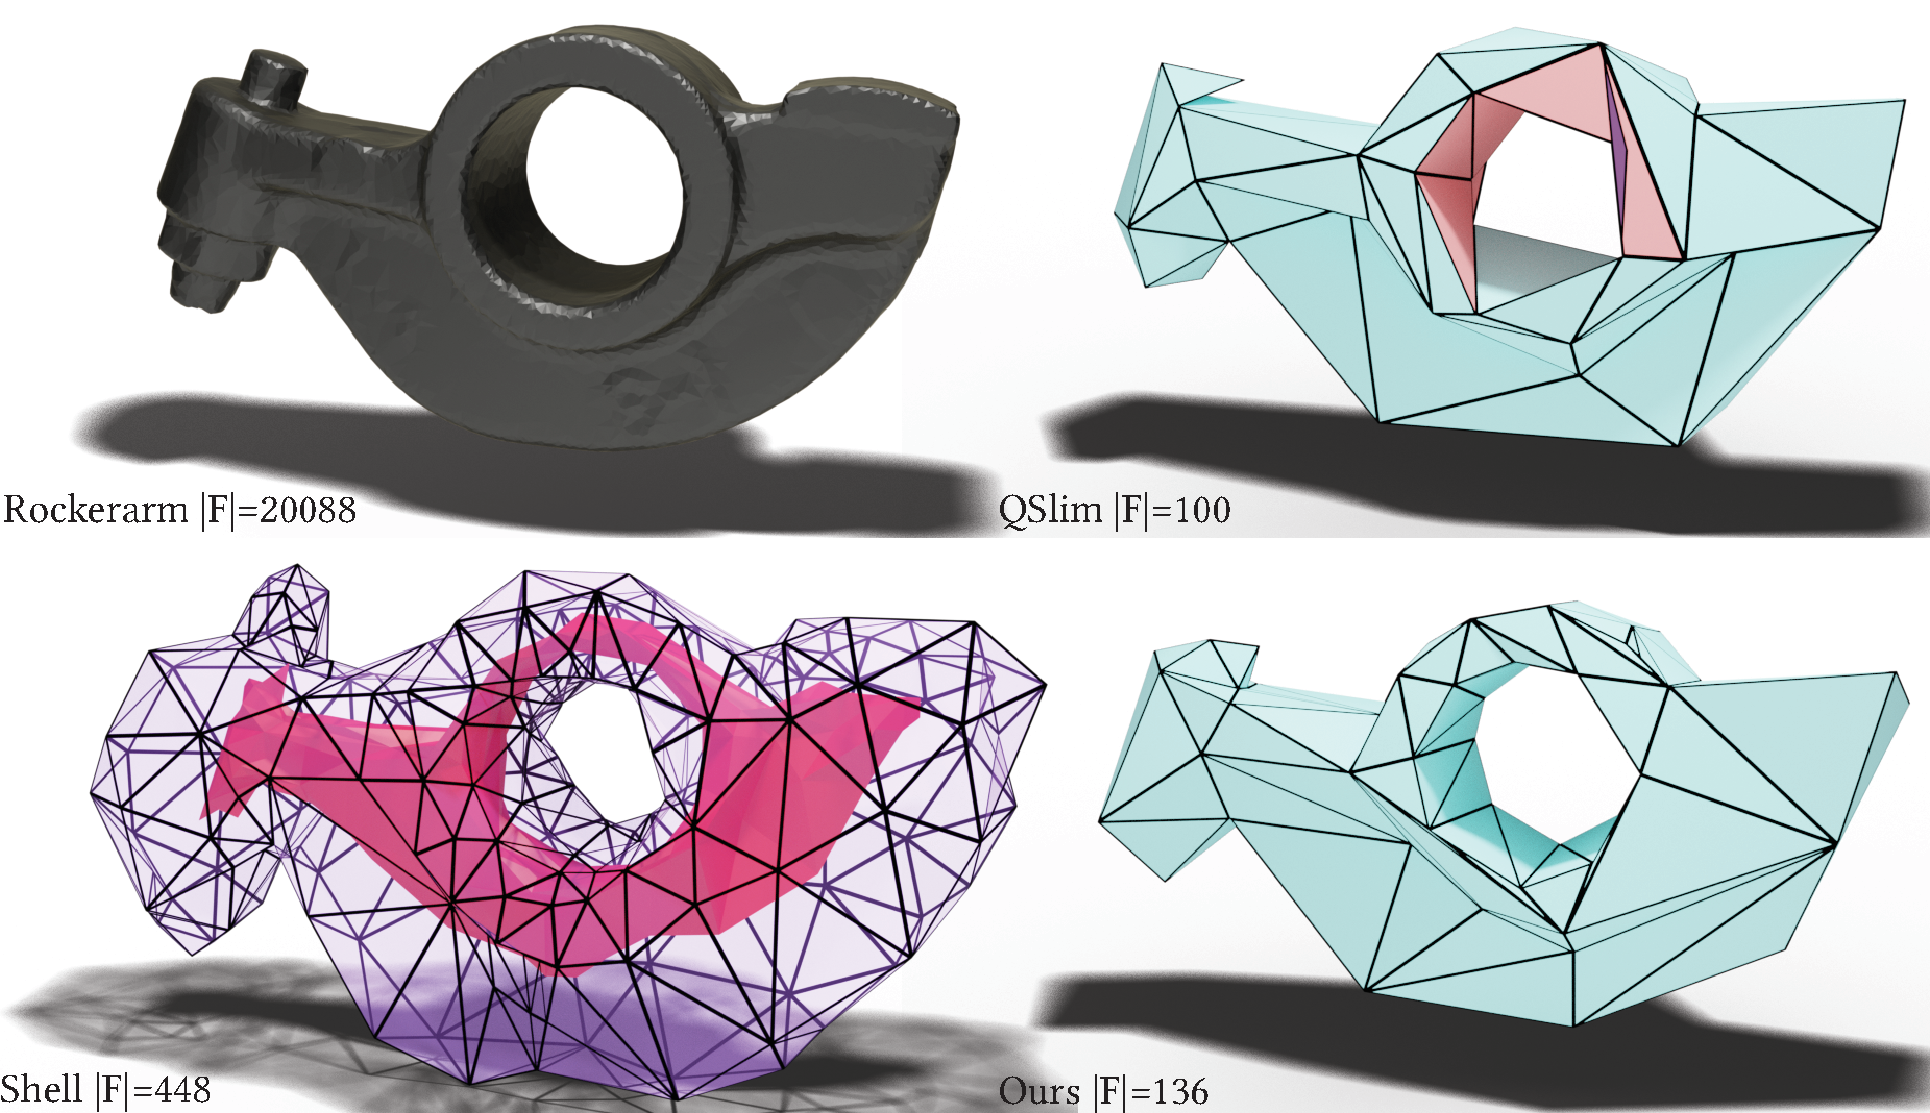
\includegraphics[width=1\linewidth]{prism-tex/figs/rockerarm_qslim}
    \caption{We attempt to simplify \protect\emph{rockerarm} (top left) from 20088 triangles to 100. QSlim~\cite{garland1998simplifying} succeeds in reaching the target triangle count (top right) but generates an output with a self-intersection (red) and flipped triangles (purple).
    With our shell constraints (bottom left), the simplification stagnates at 136 triangles, but the output is free from undesirable geometric configurations. \revision{Note that both examples use the same quadratic error metric based sceduling~\cite{garland1998simplifying}.}
    }
    % 868 Distortion Reject, 284 Intersection Reject.
    \label{prism:fig:qslim100}
    
\end{figure}

\paragraph{Remeshing}
We integrated our shell in the meshing algorithm proposed in \cite{dunyach2013adaptive} by adding envelope checks ensuring that the surface is a section after every operation. After simplification, we can use the projection operator to transfer properties between the original and remeshed surface (e.g., figures \ref{prism:fig:proxy-heat}, \ref{prism:fig:proxy-tetgen}).
%During the algorithm, we can also transfer sharp features to the current surface \DP{How is it done?} to preserve them in the remeshed surface (Figure \ref{prism:fig:sharp}).
Since the  remeshed surface is a section, a very practical side effect of our construction is that the remeshed surface is \emph{guaranteed to be free of self-intersections}, 
% \ZJ{the next sentence is commented out}
As shown in Figure~\ref{prism:fig:qslim100}, the constraints enforced through our shell prevents undesirable geometric configurations (intersections, pockets, or triangle flips).

%boundaries are preserved by our algorithm during shell construction, but cannot be simplified without breaking the bijectivity of the map. For applications such as remeshing, it is easy to allow the boundary to be simplified by enabling also the points on the boundary to move (Figure \ref{}), and the locally injective map from the remeshed surface to the input can still be used to resample attributes.


%%%%%%%%%%%%%%%%%%%%%%%%%%%%%%%%
\begin{figure}
    \centering
    \includegraphics[width=\linewidth]{prism-tex/figs/heat-in-nut}
    \caption{The heat method (right top) produces inaccurate results due to a poor triangulation (left top). We remesh the input with our method (left bottom), compute the \revision{solution of the heat method~\cite{crane2013geodesics}} on the high-quality mesh (middle bottom) and transfer the solution back to the input mesh using the bijective projection (bottom right). This process produces a result closer to the exact discrete geodesic distance \cite{mitchell1987discrete} (top middle, \revision{error shown in the histograms}).}
    \label{prism:fig:proxy-heat}
    
\end{figure}


\begin{figure}
    \centering
    \includegraphics[width=\linewidth]{prism-tex/figs/tet-knot}
    \caption{\emph{Knot} simplified with our method and tetrahedralized with TetGen. 
    The original model is converted to 1,503,428 tetrahedra (left) while the simplified surface is converted to only
    176,190 tetrahedra (right).}
    \label{prism:fig:proxy-tetgen}
    
\end{figure}


\paragraph{Proxy}
A particularly useful application of our shell is the construction of proxy domains for the solutions of PDEs on low-quality meshes. 
Additionally, by specifying the target thickness parameter (Figure~\ref{prism:fig:vary_thick}),
we are able to bound the geometry approximation error to the input as well.
Using our method,
we can (1) convert a low-quality mesh to a proxy mesh with higher quality and desired density, (2) map the boundary conditions from the input to the proxy using the bijective projection map, (3) solve the PDE on the proxy (which is a standard mesh), and (4) transfer back the solution on the input surface (Figure \ref{prism:fig:proxy-heat}). 
% \ZJ{NiT discussion is commented out below.}
\revision{Our} algorithm can be directly used to solve volumetric PDEs.
by calling an existing tetrahedral meshing algorithm between steps 2 and 3 (figures \ref{prism:fig:teaser},~\ref{prism:fig:proxy-tetgen}). 
In this case, we control the geometric error by setting the target thickness (we use 2\% of the longest edge of the bounding box).

% \begin{figure}
%     \centering
%     \includegraphics[width=1\linewidth]{prism-tex/figs/uvsphere-nit}
%     \caption{Intrinsic refinement~\cite{sharp2019navigating} cannot simplify the input mesh, while our approach can freely change the input connectivity and resolution. We can create a high-quality, isotropic triangulation of the sphere by uniformly upsampling the middle surface and projecting it to the input with our projection. Note that this mesh is a section, and we can thus transfer any attribute from the input bijectively.}
%     \label{prism:fig:uvsphere_nit}
% \end{figure}

%%%%%%%%%%%%%%%%%%%%%%%%%%%%%%%%

\begin{figure}
    \centering
    \includegraphics[width=0.9\linewidth]{prism-tex/figs/birdengine}
    \caption{The union of two meshes is coarsened through our algorithm, while preserving the exact correspondence, as shown through color transfer.}
    \label{prism:fig:birdengine}
    
\end{figure}

\paragraph{Boolean Operations}
The mesh arrangements algorithm enables the robust and exact (up to a final floating-point rounding) computation of Boolean operations on PWN meshes \cite{zhou2016mesh}. 
However, the produced meshes tend to have low triangle quality that might hinder the performance of \revision{downstream} algorithms. %using them to evaluate large CSG trees. 
By interleaving a remeshing step performed with our algorithm after every operation, we ensure  high final quality and more stable runtime. The composition of the bijections enables us to transfer properties between different nodes of the CSG tree (Figure~\ref{prism:fig:birdengine}).%\ZJ{I am not sure we want to talk about CSG tree, since we did not really have it.}


%%%%%%%%%%%%%%%%%%%%%%%%%%%%%%%%
\begin{figure}
    \centering
    \includegraphics[width=0.95\linewidth]{prism-tex/figs/bunny-displacement}
    \caption{Top: an input mesh decimated to create a coarse base mesh, and the details are encoded in a displacement map (along the normal) with correspondences computed with Phong projection \cite{kobbelt1998interactive}. Bottom: the decimation is done within our shell while using the same projection as above. With our construction, this projection becomes bijective (Appendix \ref{app:bilinear}), avoiding the artifacts visible on the ears of  the bunny in the top row.}
    \label{prism:fig:displacement-mapping}
    
\end{figure}
\paragraph{Displacement Mapping}
The middle surface of the shell is a coarse triangular mesh that can be directly used to compress the geometry of the input mesh, storing only the coarse mesh connectivity and adding the details using normal and displacement maps (Figure \ref{prism:fig:displacement-mapping}). A common way to build such displacement is to project \revision{\cite{kobbelt1998interactive,collins2002mesh}} the dense mesh on the coarser version. As shown in Appendix \ref{app:bilinear}, our method guarantees that this natural projection is also bijective as long as the coarse mesh is a section. This 
\revision{alleviates the loss of information}
% ensures that no information is lost 
even on challenging geometry configurations, and our shell can thus be used to automate the creation of projection cages and displacement maps.
%%%%%%%%%%%%%%%%%%%%%%%%%%%%%%%%

% \paragraph{Boundary Layers}
% Boundary layer meshes are commonly used in computational fluid dynamics. Our algorithm can be used to generate them by sampling the inverse projection operator at different heights to construct a set of thinner prismatic layers (Figure \ref{}). The volume outside of the shell can then be meshed using TetGen \cite{}.


%%%%%%%%%%%%%%%%%%%%%%%%%%%%%%%%
\begin{figure}
    \centering
    \includegraphics[width=\linewidth]{prism-tex/figs/chain-lizard}
    \caption{Two volumetric chainmail textures (right) are applied to a shell (bottom left) constructed from the \emph{Animal} mesh (top left).
    The original UV coordinates are transferred using our projection operator.}
    \label{prism:fig:volumetric-textures}
    
\end{figure}
\paragraph{Geometric Textures.}
The inverse projection operator provides a 2.5D parametrization around a given mesh and can be used to apply a volumetric texture (Figure \ref{prism:fig:volumetric-textures}).
Note that we build the volumetric texture on the simplified shell, while still being able to bijectively transfer the texture coordinates.
%We also believe our discussion on the valid shells (Section~\ref{sec:singularities}) will be the building block for a robust shell map algorithm.}



%%%%%%%%%%%%%%%%%%%%%%%%%%%%%%%%%%%%%%
%%%%%%%%%%%%%%%%%%%%%%%%%%%%%%%%%%%%%%
%%%%%%%%%%%%%%%%%%%%%%%%%%%%%%%%%%%%%%



\section{Variants}\label{sec:variants}


\paragraph{Input with Self-Intersections}
Up to this point, we assumed that our input meshes are without self-intersections. This requirement is necessary to guarantee a bijection between any section (e.g., the input mesh) and the middle surface. Such bijection is essential for a key target application, the transfer of boundary conditions for solving PDEs on meshes or mesh-bounded domains. 

However, our method can be easily extended to meshes containing self-intersections, broadening the class of meshes it can be applied to, at the cost of making the resulting shell usable in fewer application scenarios: for example, if it is used for remeshing, it will likely generate a new surface that still contains self-intersections.

If $\T$ contains self-intersections, our algorithm can be trivially extended to generate a shell which will be \emph{locally injective}, and the bijectivity of the mapping between sections still holds but with respect to the immersion. The only change required is to modify the invariance checks (Section \ref{sec:optimization}): we have to replace the global intersection check with checking whether local triangles overlap with the current prisms. Figure~\ref{prism:fig:intersect-leg} shows an example of a mesh $\T$ with self-intersections, the generated shell, and the isolines of geodesic transferred on the coarser middle surface.
\begin{figure}
    \centering
    \includegraphics[width=\linewidth]{prism-tex/figs/leg-intersect}
    \caption{An example of a shell built around a self-intersecting mesh.}
    \label{prism:fig:intersect-leg}
    
\end{figure}


\begin{figure}
    \centering
    \includegraphics[width=\linewidth]{prism-tex/figs/armadillo_cage}
    \caption{The \protect\emph{Armadillo} model with four nested cages. We create a shell from the original mesh, and then rerun our algorithm on the outer shell to create the other three layers. Note that all layers are free of self-intersections, and we have an explicit bijective map between them.}
    
    \label{prism:fig:nested-cages}
\end{figure}

\paragraph{Resolving Shell Self-Intersections}
\label{sec:postprocessing}
% During initialization and optimization, we forbid the top and bottom surfaces to intersect with $\T$. However, the optimized shell $\S$ might have self-intersections, i.e. there can be a point in ambient space contained in more than one prism.  While this is not an issue for our shell construction and optimization (which is defined inside every prism), this is not desirable for specific applications 
% where the offset surface we created for geometry processing tasks. 
For certain applications it might be preferable to have a shell whose  \revision{top and bottom surfaces do} not self-intersect:
for example, in the construction of nested cages \cite{sacht2015nested} (useful for collision proxies and animation cages), we want to iteratively build nested shells while ensuring no intersections between them (Figure \ref{prism:fig:nested-cages}). 
With a small modification, our algorithm can be used to generate nested cage automatically and robustly, with the additional advantage of being able to map any quantity  bijectively across the layers and to the input mesh. In contrast, \cite{sacht2015nested}
does not provide guarantees on the success (e.g., the reference implementation of \cite{sacht2015nested} fails on Figure~\ref{prism:fig:qslim_naive}, probably due to the presence of a singularity). 
\begin{figure}
    \centering
    \includegraphics[width=0.8\linewidth]{prism-tex/figs/camel}
    \caption{After optimization, the shell may self-intersect (left). Our postprocessing can be used to extract a non-selfintersecting shell, which is easier to use in downstream applications (right).}
    \label{prism:fig:shell_shrinking-cages}
    
\end{figure}

To resolve the self-intersections of the top (bottom) surface, we identify the regions covered by more than one prism by explicitly testing intersections between the tetrahedralized prisms, accelerated using \cite{zomorodian2000fast}. For every detected prism, we reduce the thickness by 20\%, and iterate until no more intersections are found. 
Differently from the procedure in Section \ref{sec:initialization}, where reducing the thickness of the shell always maintains the validity of the shell, at this stage, the shrinking of the shell may make the shell invalid, since $\T$ may not be contained anymore in $\S$. 
Whenever this happens, we perform one step of red-green refinement \cite{bank1983some} on the regions we wish to thin, and we iterate until we succeed. This procedure is guaranteed to terminate since, on the limit of the refinement, the middle surface will be geometrically identical to $\T$, and thus Theorem \ref{thm:thickness} holds.
In the worst case, the procedure terminates when the size of triangles on the middle surface is comparable to the input; then no refinement is required to shrink below the minimum separation of the input.
Figure~\ref{prism:fig:shell_shrinking-cages} shows how the intersecting shell between the legs of the camel can be shrunk to generate an intersection-free shell. 



\begin{figure}
    \centering
    \includegraphics[width=0.9\linewidth]{prism-tex/figs/blocks}
    \caption{We generate a pinched shell for a model with a singularity (left).
    Optionally, we can complete the shell using our Boolean construction.}
    \label{prism:fig:singularity-boolean}
    
\end{figure}


\paragraph{Pinching Alternative.} For certain applications, such as boundary layer meshing, it is necessary to have a shell with non-zero thickness everywhere, including at singularities, and it is tolerable to lose bijectivity at the vicinity of a singularity. For these cases, we propose a Boolean construction to \emph{fill} the shell around singularities, and to extend the projection operator $\P$ inside these regions. That is, every point in the filled region will project to the singularity. 
% An unavoidable (with our definition of projection) side effect of this construction is that $\P$ loses local injectivity.

Without loss of generality, let us assume that $\T$ has a single singularity (Figure \ref{prism:fig:singularity-boolean}). We initially construct a pinched shell, with zero thickness at the singularity, construct a valid shell (Section~\ref{sec:method}), and then perform a corefinement~\cite{corefinement} between a tetrahedron (centered at the singularity and whose size is smaller than the minimal thickness of the neighboring vertices) and the shell. The result of the corefinement operation (Figure \ref{prism:fig:singularity-boolean} middle) consists of triangles belong to the tetrahedron, or the shell surface. The remaining part of the tetrahedron is a star-shaped polyhedron with the singularity in its kernel, and sharing a part of its boundary with the shell. This polyhedron can be easily tetrahedralized by connecting its triangulated boundary faces (one of them is highlighted in red in Figure \ref{prism:fig:singularity-boolean} middle) with the singularity. For every point $p$ in these tetrahedra, the projection operator $\P$ projects $p$ to the singularity. The remaining triangles are divided into two groups: 
the triangles with only one new vertex complete the degenerate prisms (one of them is highlighted in blue in Figure \ref{prism:fig:singularity-boolean} middle), 
while the others map to the edges they are attached to.






\section{Limitations and Remarks}

Currently, our algorithm is limited to manifold and orientable surfaces: its extension to non-manifold and/or non-orientable meshes is a potential venue for future work. With such an extension, the integration of shells with robust tetrahedral meshers \protect{\cite{hu2018tetrahedral, Hu:2019:fTetWild}} would allow to solve PDEs on imperfect triangle meshes without ever exposing the user to the volumetric mesh, allowing them to directly work on the boundary representation to specify boundary conditions and to analyze the solution of the desired PDE.
%
{Since we rely on the additional checks for the bijective constraints, our method is slower than classical surface mesh adaptation algorithms and it is not suitable for interactive applications.}

{Integrating our approach into existing mesh processing algorithms might lose some of their guarantees or properties since our shell might prevent some local operations.
Other surface processing algorithms guarantee some properties under some regularity assumptions on the input, which might not hold when our bijective constraints are used. 
For example, 
%mesh fairing using Willmore flow \cite{bobenko2005discrete} might not converge to the true smooth solution,
QSlim \cite{garland1997surface} might not be able to reach the desired target number of vertices and \cite{dey2010polygonal} might not be able to achieve the bounded aspect ratio.}
{A practical limitation is that integrating our approach into existing remeshing or simplification implementations requires code level access.}

{Our shell is ideal for triangle remeshing algorithms employing incremental changes: not every geometry processing algorithm requiring a bijective map can use our construction. For example, it is unclear how isosurface-extraction methods \cite{hass2020approximating} could use our shell or how global parametrization algorithms \cite{kraevoy2004cross,Schreiner:2004,alliez2003isotropic,bommes2013quad} could benefit from our method since they already compute a map to a common domain.}



We introduce an algorithm to construct shells around triangular {meshes} and define bijections between surfaces inside the shell. We proposed a robust algorithm to compute the shell,
validated it on a large collection of models, and demonstrated its practical applicability in common applications in graphics and geometry processing. 


We believe that many applications in geometry processing could benefit from bijectively mapping spatially close surfaces, and that the idea of using an explicit mesh as a common parametrization domain could be extended to the more general case of computing cross-parametrizations between arbitrary surfaces. To foster research in this direction, we will release our reference implementation as an open-source project.





\chapter{Bijective and Coarse High-Order Tetrahedral Meshes}
\label{chp:curve}

\begin{figure}
    \centering
    \includegraphics[width=\linewidth]{curve_meshing_in_shell_tex/figs/teaser}
    \caption{Our pipeline starts from a dense \emph{linear} mesh with annotated features (green), 
    which is converted in a curved shell filled with a high-order mesh. The region bounded by the shell is then tetrahedralized with linear elements, which are then optimized. Our output is a coarse, yet accurate, curved tetrahedral mesh ready to be used in FEM based simulation. Our construction provides a bijective map between the input surface and the boundary of the output tetrahedral mesh, which can be used to transfer attributes and boundary conditions.}
    \label{bichon:fig:teaser}
\end{figure}

\section{Introduction}

Piecewise linear approximations of surfaces are a popular representation for 3D geometry due to their simplicity and wide availability of libraries and algorithms to process them. However, dense sampling is required to faithfully approximate smooth surfaces. 
%
Curved meshes, that is, meshes whose element's geometry is described as a high-order polynomial, are an attractive alternative for many applications, as they require fewer elements to achieve the same representation accuracy of linear meshes. In particular, curved meshes have been shown to be effective in a variety of simulation settings in mechanical engineering, computational fluid dynamics, and graphics. Despite their major benefits, they are not as popular as linear meshes: We believe that {one of} the main reason for their limited usage is the lack of an automatic, robust way of constructing them. 

While robust meshing algorithm exists for volumetric linear tetrahedral meshing, there are few algorithms for curved meshes, and even fewer of them having either a commercial or open-source implementation (Section \ref{sec:related}). Only {a} few algorithms work directly on arbitrary triangle meshes (most of them require the input geometry to be either a CAD file or an implicit function), and none of them can reliably process a large collection of 3D models. 

We propose the first robust and automatic algorithm to convert dense piecewise linear triangle meshes (which can be extracted from scanned data, volumetric imaging, or CAD models) into coarse, curved tetrahedral meshes equipped with a bijective map between the input triangle mesh and the boundary of the tetrahedral mesh. Our algorithm takes advantage of the recently proposed bijective shell construction \cite{jiang2020bijective} to allow joint coarsening, remeshing, and curving of the dense input mesh, which we extend to support feature annotations.
Our outputs are guaranteed to have a self-intersection free boundary and the geometric map of every element is guaranteed to be bijective, an important requirement for FEM applications.

The key ingredient of our algorithm is the separation of the curved volumetric meshing problem into a near-surface, surface curving problem, followed by a restricted type of linear volumetric meshing. 

% This is repetitive
%For the former, we use prismatic elements to create a valid parametrization close to the surface, and use it to ensure validity during mesh coarsening and curving.

% \TS{i dont think we should state this here}
% An important subproblem, of independent interest, that we tackle in this paper is constrained linear volumetric meshing (i.e. fill the interior of closed, non self-intersecting triangle mesh without refining it), for which we propose a simple and robust algorithm that is inspired by the TetWild algorithm \cite{hu2018tetrahedral}.

We believe that our curved meshing algorithm will enable wider adoption of curved meshes, as it will provide a way to automatically convert geometric data in multiple formats into a coarse tetrahedral mesh readily usable in finite element applications. To showcase the benefits of our approach we study 2 settings: (1) we show that a coarse proxy mesh can be used to compute non-linear deformations efficiently and transfer them onto a high-resolution geometry, targeting real-time simulation (Figure~\ref{bichon:fig:teaser}), and (2) 
we show that our meshes are ready to use in downstream FEM simulations.

% Additionally, we show that the boundary of our tetrahedral mesh, which is a curved (yet only $C^0$) surface mesh is useful for automatically generating assets for real-time rendering pipelines, despite the lack of normal continuity across patches.
% \DP{Or maybe not? Let's see.}

We validate the reference implementation of our approach on a large collection of more than 8000 geometrical models, which will be released as an open-source project to foster the adoption of curved meshes in academia and industry.

Our contributions are:
\begin{itemize}
    \item An algorithm to convert dense piecewise linear meshes into coarse curved volumetric meshes while preserving a bijective map with the input and bounding the approximation error.
    \item An extension of the bijective shell construction algorithm to support feature {annotations}.
    \item An algorithm for conforming tetrahedral meshing without allowing refinement on the boundary, but allowing internal Steiner points.
    % \item A reusable open-source implementation of our algorithm evaluated on a large scale benchmark.
    \item A large-scale dataset of high-order tetrahedral meshes.
\end{itemize}

\subsection{Variation from the Original Algorithm}
To extend the shell formulation in~\ref{chp:shell} to accommodate for feature preservation (Section \ref{cumin:sec:features-pres}), 
we modify the definition of a valid section (Chapter~\ref{chp:shell} Definition 3.1), 
by relaxing the intersection between a triangle and a prism in the discrete case. That is, we do not consider the prism to be intersecting a triangle if they share only one vertex of the triangle; we also ignore the intersection if they intersect on a feature edge on opposite sides. The bijectivity and validity condition of the shell projection trivially holds.

%%%%%%%%%%%%%%%%%%%%%%%%%%%%%%%%%%%%%%%%%%%
%%%%%%%%%%%%%%%%%%%%%%%%%%%%%%%%%%%%%%%%%%%

\begin{figure}
    \centering
    \includegraphics[width=.8\linewidth]{curve_meshing_in_shell_tex/figs/illustrations/input-output.pdf}
    \caption{Input triangle mesh $\M$ and points $\P$. Output curved tetrahedral mesh $\T^k$ and bijective map $\phi^k$.}
    \label{bichon:fig:input-output}
\end{figure}

\section{Curved Tetrahedral Mesh Generation}\label{cumin:sec:curved-pipeline}



\paragraph{Input.}
The input of our algorithm is a collection of oriented manifold, watertight, self-intersection-free triangle mesh $\M=(V,F)$, and a set of points $p_i\in\P$ (possibly empty) on the surface of $\M$ (Figure~\ref{bichon:fig:input-output}, left) where the distance bound $\varepsilon$ is prescribed. The collection $\M$ must be consistently oriented such that it is the boundary of an oriented 3-manifold.
A set of edges can also be optionally provided as annotated features (Section~\ref{cumin:sec:features-pres}).

\begin{figure}
    \centering
    % \includegraphics[width=.6\linewidth]{curve_meshing_in_shell_tex/figs/nodes}\hfill
    % \includegraphics[width=.37\linewidth]{curve_meshing_in_shell_tex/figs/gmapping}
    \includegraphics[width=\linewidth]{curve_meshing_in_shell_tex/figs/illustrations/high-order.pdf}
    \caption{Lagrange nodes on the reference element $\hat \tau$ for different $k=1,2,3$, and example of geometric mapping $g$.}
    \label{bichon:fig:high-order}
\end{figure}

\paragraph{Output.}
The output of our algorithm is a tetrahedral mesh $\T^k = (V^k,T^k)$ of order $k$. 
Formally, each tetrahedron $\tau\in T^k$ is defined through the \emph{geometric map} from the reference tetrahedron $\hat \tau$,
\begin{equation}\label{eq:gmap}
g^\tau = \sum_{j=1}^n c_j^\tau L_j(\hat u,\hat v,\hat w),
\end{equation}
where $\hat u,\hat v,\hat w$ are the local coordinates of a point in $\hat \tau$, $c_j^\tau$ are the control points for a tetrahedron $\tau$, and $L_j$ are polynomial bases (typically Lagrange bases).
For two tetrahedra $\tau_1$ and $\tau_2$ 
of $T^k$ sharing a face $F$, the restriction of the maps $g^{\tau_i}$, $i=1,2$, to $F$ coincide.
Figure~\ref{bichon:fig:high-order} shows the position of the control points $c_j$ on the reference element for $k=1,2,3$ for the Lagrange bases. We call the tetrahedralization of a curved mesh $\T^k$ \emph{positive} if $\det(J_{g^\tau}) > 0$ everywhere on every $\tau$. 
% That is, we require that the geometric mapping $g^T$ is bijective for every tetrahedron \DP{I don't think this is true, the implication holds the other way, discuss.} \DZ{Indeed this is obviously not true except in the linear case; positive Jacobian only guarantees local injectivity; a sufficient condition is that the map is bijective on the boundary}. 
In particular, for $k=1$, since $g$ is affine, $J_{g^\tau}$ is constant and the positivity reduces to the positive orientation of the vertices \cite{shewchuk1997adaptive}.

Note that, while bijectivity of the geometric map $g^\tau$ implies positivity, the reverse is not true. 
Therefore, our algorithm not only checks for $\det(J_{g^\tau}) > 0$, but also ensures that the boundary $\partial\T^k$ does not intersect; we show in section~\ref{cumin:sec:bij-proof} that these two conditions guarantee the bijectivity of $g^\tau$.
Furthermore, our algorithm ensures that the distance from any point in $\P$ to $\partial\T^k$ (the surface of $\T^k$) is smaller than an user-controlled parameter $\varepsilon$.

\begin{figure}
    \centering\small
    \includegraphics[width=0.23\linewidth]{curve_meshing_in_shell_tex/figs/bunny/0001}\hfill
    \includegraphics[width=0.23\linewidth]{curve_meshing_in_shell_tex/figs/bunny/0004}\hfill
    \includegraphics[width=0.23\linewidth]{curve_meshing_in_shell_tex/figs/bunny/0003}\hfill
    \includegraphics[width=0.23\linewidth]{curve_meshing_in_shell_tex/figs/bunny/0002}\par
    \parbox{.23\linewidth}{\centering 0 points.}\hfill
    \parbox{.23\linewidth}{\centering 200 points.}\hfill
    \parbox{.23\linewidth}{\centering 500 points.}\hfill
    \parbox{.23\linewidth}{\centering 1000 points.}
    \caption{Effect of the choice of the set $\P$ on the output.}
    \label{bichon:fig:points-effect}
\end{figure}



We are not assuming anything on $\P$: a sparse set of points will generate a mesh less faithful to the input geometry, while a dense sampling computed for instance with Poisson disk sampling~\cite{bowers2010parallel} will prevent the surface from deviating too much (Figure~\ref{bichon:fig:points-effect}).


Our algorithm guarantees that the tetrahedralization is positive and that $\partial\T^k$ does not have self-intersections. 
It also aims at coarsening {$\T^k$} as much as possible while striving to obtain a good geometric quality. 
To reliable fit $\partial \T^k$ to $\M$ we require a bijective map
\[
\phi^k \colon \M \to \partial \T^k
\]
from the input $\M$ to the surface of $\T^k$ (Figure~\ref{bichon:fig:input-output} right). Our algorithm also generates this map and exposes it as an output for additional uses, such as attribute transfer. Note that, since we build upon the shell construction in~\ref{chp:shell}, we also {guarantee} $\partial\T^k$ is homeomorphic and topology-preserving with respect to $\M$ (Figure~\ref{bichon:fig:intersection}).


\begin{figure}
    \centering
    % \includegraphics{}
    \includegraphics[width=0.9\linewidth]{curve_meshing_in_shell_tex/figs/intersection-free.pdf}\hfill
    \caption{Our algorithm maintains {free of} intersection even on challenging models, without the need of setting adaptive threshold.}
    \label{bichon:fig:intersection}
\end{figure}


%For each edge provided in the feature annotation list, 
%there exists one curved edge in the output mesh, 
%where the marked edge is in bijective correspondence to a segment in the curved edge.


To simplify the explanation{,} we use the bar $\overline{\phantom{M}}$ to represent quantities on the \emph{straight} linear shell, the tilde $\widetilde{\phantom{M}}$ for the \emph{curved} shell, and hat $\hat{\phantom{M}}$ for the reference elements (e.g., $\overline P$ is the prism on {the} straight coarse shell, $\widetilde P$ is the curved prism, and $\hat P$ is the prism on the reference configuration).


\begin{definition}\label{def:curved-mesh}
We call a curved mesh $\T^k$ and its mapping $\phi^k$ to $\M$ \emph{valid} if it satisfies the following conditions:
\begin{enumerate}
    \item $\phi^k$ is bijective;
    \item the distance between any $p\in\P$ and $\partial\T^k$ is less than $\varepsilon$;
    \item $\T^k$ is positive (i.e., every geometric map $g^\tau$ has positive Jacobian's determinant).
\end{enumerate}
\end{definition}

\paragraph{Overview.} 
Our algorithm starts by creating a valid mesh (i.e., it satisfies~\ref{def:curved-mesh}), then it performs local operations (section~\ref{app:local-ops}) to improve $\T^k$ (i.e., coarsen it and improve its quality) while ensuring all the conditions remain valid with respect to local modification. 
To achieve this goal, our algorithm uses two stages: (1) curved shell generation and (2) tetrahedral mesh generation and optimization.

\begin{figure}
    \centering
    \includegraphics[width=\linewidth]{curve_meshing_in_shell_tex/figs/illustrations/pipeline.pdf}
    \caption{Overview of curved mesh generation pipeline.}
    \label{bichon:fig:pipeline}
\end{figure}

\paragraph{Stage 1: Curved Shell Construction.}
In the first stage (Section~\ref{cumin:sec:high-order}) we extend the shell construction of~\ref{chp:shell} by combining the shell projection $\Pi$ with {a} high-order mapping 
\[
\psi^k \colon \prS \to \PS.
\]
We start form the \emph{valid} shell $\PS$ constructed from the input mesh $\M$ (i.e., $\M$ is a section $\PS$). We call $\PS$ a \emph{\ps{}} and call the prismatic projection $\Pi$. Together with the construction of $\PS$, we build an order $k$ \emph{curved prismatic shell} $\prS$ that defines a curved layer around $\M$ and a \emph{bijective} map $\psi^k$ between $\prS$ and $\PS$ (Figure~\ref{bichon:fig:pipeline}, first three figures) that ensures that the distance between $\M$ and $\partial\T^k$ is smaller than $\varepsilon$ (Section~\ref{cumin:sec:distance}). That is, $\phi^k(p) < \varepsilon$ for any $p\in\P$. (Note that we do not require $\M$ to be a section of $\prS$.)

To facilitate the volumetric meshing in the next stage (Section~\ref{cumin:sec:tets}), we restrict the top and bottom surface of $\prS$ to be linear (independently from the order of $\psi^k$). The final output of this first stage is a high-order volumetric shell,
a bijective mapping $\phi^k = \Pi \circ \psi^k$,
and a \emph{positive} tetrahedralization of $\prS$ with flat boundary. In other words, the tetrahedralization of $\prS$ satisfies~\ref{def:curved-mesh}.

\paragraph{Stage 2: Tetrahedral Mesh Generation.}
In the second stage (Section~\ref{cumin:sec:tets}) we use boundary-conforming tetrahedralization to connect the top and bottom surface of $\prS$ with a background tetrahedral mesh, thus generating a \emph{positive} order $k$ tetrahedralization $\T^k$ of a bounding box around the input, which we can further optimize with local operations to improve its quality  (Figure~\ref{bichon:fig:pipeline}, last two figures). % Note that this pipeline  decouples the surface generation and feature preservation problem from the conforming volumetric tassellation, enabling us to tackle these two challenges independently.


To ensure that our first condition is satisfied{,} we define the mapping $\phi^k$ as a composition of several mappings{,} which we ensure are bijective. 
For the second condition, we initialize our construction with $\phi^k$ {as} the identity, {and} thus, the distance at the sample points is zero. 
After every operation, we recompute the distance and ``undo'' the operation if the distance becomes larger than $\varepsilon$. To ensure that the last condition holds, we rely on checking if all prisms (linear and curved) have positive geometric mapping, which {ensures} that they can be tetrahedralized with a positive tetrahedralization. 
Ensuring the condition while coarsening $\M$ {allows} us to generate a coarse \emph{curved} tetrahedral mesh $\T^k$ and the \emph{bijective} map $\phi^k$ to the input mesh $\M$.


\subsection{High-order Shells}\label{cumin:sec:high-order}
To simplify the explanation, we first focus on the case where $\varepsilon = \infty$, that is, we aim at generating {an} as-coarse-as-possible curved mesh. Note that, the trivial solution (i.e., a single tetrahedron) is not necessary a valid $\T^k$ since it would be impossible to build the bijective mapping $\phi^k$.

The output of~\ref{chp:shell} is a coarse shell $\PS$ with {a} piecewise linear middle surface. To curve it, we construct a shell $\prS$ and the bijective map $\psi^k$ while constructing $\PS$. 
The shell $\prS$ is constructed warping every prism $\widetilde P$ of $\prS$ with $\psi^k$. Since we define $\phi^k$ as  $\Pi \circ \psi^k$, and $\Pi$ satisfies the first two conditions~\ref{def:curved-mesh}, we only need to ensure that $\psi^k$ is bijective, for $\phi^k$ to be bijective.  We define the mapping $\psi^k = \overline\omega\circ(\widetilde\omega^k)^{-1}$ {through} two {cross-parametrization} maps from the reference prism $\hat P$: 
\[
% \text{(1) } 
\overline\omega \colon \hat P \to \overline P, \qquad
% \text{(2) } 
\widetilde\omega^k \colon \hat P \to \widetilde P.
\]

Both mappings $\overline\omega$ and $\widetilde\omega^k$ are defined as the tensor product between the base triangular mapping (high-order for $\widetilde\omega^k$) and pillar's {barycentric} heights. That is, for a prism $\widetilde P$
\[
\widetilde\omega^k (\hat u,\hat v, \hat h) = 
% \sum_{i=1}^3 
\sum_{j=1}^n c_j^P L_j(\hat u,\hat v) \big((1-\hat u - \hat v)  h_1^{\widetilde P}+ \hat u h_2^{\widetilde P} + \hat v  h_3^{\widetilde P}\big)\hat h,
\]
where $\hat u,\hat v,\hat h$ are the barycentric coordinates in the reference prism, $c_j$ the control points of a triangle, $h_i^{\widetilde P}$ the three pillars heights, and $L_j$ a triangle polynomial basis.
By ensuring that $\psi^k$ is bijective, we guarantee that any curved tetrahedralization of a prism $\widetilde P$ will be a valid tetrahedralization of $\prS$.

We note that to decouple the following tetrahedral mesh generation and the curved shell generation, we ensure that $\widetilde\omega^k$ maps the top and bottom face of the curved prism $\widetilde P$ to a linear triangle.

After each local operation, we generate samples $\hat s_i, i=1,\dots,m$ on the parametric base of the prism $\hat P$ and use $\Pi^{-1}\circ \overline\omega$ to map $\hat s_i$ back to $\M$ and $\widetilde \omega^k$ to map them to $\partial\T$. Using the mapped point we solve
\[
\min_{c_i} \sum_{i=1}^m \|
(\Pi^{-1}\circ \overline\omega)(\hat s_i) - 
\widetilde \omega[c_i]^k(\hat s_i)
\|_2^2,
\]
where $c_i$ are the control points of $\widetilde\omega^k$. As $\widetilde \omega[c_i]^k(\hat s_i)$ is a linear function of $c_i$. This is a quadratic optimization problem.
The control points of the top and bottom surface are fixed to ensure that $\widetilde\omega^k$ maintains the two surfaces as linear. We validate the bijectivity of
$\widetilde\omega^k$ by checking positivity of the determinant~\cite{johnen2013geometrical} and that the top and bottom surfaces are intersection free. The intersection is simplified in our case since fast and exact algorithms\cite{guigue2003fast} are available since the top and bottom surfaces stay linear.



\begin{figure}
    \centering\small
    % \includegraphics{}
    \includegraphics[width=.23\linewidth]{curve_meshing_in_shell_tex/figs/fish/fish002}
    \hfill
    \includegraphics[width=.23\linewidth]{curve_meshing_in_shell_tex/figs/fish/0003}\hfill
    \includegraphics[width=.23\linewidth]{curve_meshing_in_shell_tex/figs/fish/0001}\hfill
    \includegraphics[width=.23\linewidth]{curve_meshing_in_shell_tex/figs/fish/0004}\par
    \parbox{.23\linewidth}{\centering Input}\hfill
    \parbox{.23\linewidth}{\centering $\varepsilon =5\times 10^{-3}$}\hfill
    \parbox{.23\linewidth}{\centering $\varepsilon =  10^{-3}$}\hfill
    \parbox{.23\linewidth}{\centering $\varepsilon = 5\times 10^{-4}$}
    \caption{A model simplified with different distances.}
    \label{bichon:fig:distance}
\end{figure}

\subsection{Distance Bound}\label{cumin:sec:distance}

In the previous section, we explained how to generate a curved shell $\prS$ that satisfies~\ref{def:curved-mesh}. To ensure that the middle surface of $\prS$ has a controlled distance from the points in $\P$, we interleave a distance check in the construction of $\widetilde\omega^k$ after each local operation. Formally, after every local operation we use the mapping $\phi^k$ to map every point $p_i\in\P$ to $\widetilde p_i = \phi^k(p_i)$ a point on the coarse curved middle surface of $\prS$ and, if $\|p_i-\widetilde p_i\| \geq \varepsilon$ we reject the operation. The initial shell is trivially a valid initialization as $\phi^k$ is identity and thus, the distance is zero. Note that, $\widetilde p_i$ is not necessarily the closest point to $p_i$ on $\partial\T$, thus $\|p_i-\widetilde p_i\|$ is an upper bound on the actual pointwise distance. Figure~\ref{bichon:fig:distance} shows the effect of the distance bound on the surface; a small distance will lead to a denser mesh with more details, while a {large} one will allow for more coarsening.



%%%%%%%%%%%%%%%%%%%%%%%%%%%%%%%%%%%%%%%%%%%%%%%%%%%%%%%%%%%%%%%%
%%%%%%%%%%%%%%%%%%%%%%%%%%%%%%%%%%%%%%%%%%%%%%%%%%%%%%%%%%%%%%%%
\subsection{Tetrahedral Meshing}\label{cumin:sec:tets}

The outcome of the previous stage is a curved tetrahedralization of $\prS$ that closely approximates $\M$ with linear (``flat'') boundaries. We now consider the problem of filling its interior (and optionally its exterior) with a tetrahedral mesh, a problem known as  \emph{conforming boundary preserving} tetrahedralization. 

%After the linear tetrahedralization, we have a valid (according to Definition~\ref{def:curved-mesh}) output which we further improve by performing local operations on the curved mesh.

\begin{figure}
    \centering
    % \includegraphics[width=.39\linewidth]{curve_meshing_in_shell_tex/figs/tet12}\hfill
    % \includegraphics[width=.39\linewidth]{curve_meshing_in_shell_tex/figs/tet34}\hfill
    % \includegraphics[width=.19\linewidth]{curve_meshing_in_shell_tex/figs/tet5}
    \includegraphics[width=\linewidth]{curve_meshing_in_shell_tex/figs/illustrations/conforming-overview.pdf}
    \caption{Two dimensional overview of the five steps of our boundary preserving tetrahedral meshing algorithm.}
    \label{bichon:fig:conforming-overview}
\end{figure}

Several solution exists for this problem (Section~\ref{cumin:sec:rel:linear}) and the most common implementation is TetGen~\cite{tetgen}. Most algorithms refine the boundary, which allows {deriving} bounds on the quality of the tetrahedral mesh. However, in our setting, this is problematic, as any change will have to be propagated to the curved shell. To avoid coupling the volumetric meshing problem with the curved shell coarsening, while technically possible it is very challenging to implement robustly, we opt for using a tetrahedral meshing algorithm that preserves the boundary exactly. Not many algorithms support this additional constraint, the only one with a public implementation is the widely used TetGen algorithm. However, we discovered that, when this option is used, it suffers from robustness issues.
%
To solve this problem in our specific setting, we propose in the following five step algorithm (Figure~\ref{bichon:fig:conforming-overview}) taking advantage of the availability of a shell, based on the  TetWild~\cite{hu2018tetrahedral} algorithm.

\paragraph{Step 1.}
To generate a boundary preserving linear mesh, we first exploit the shell to extrude the bottom surface $B$ (and top $T$) {further} by a positive (potentially small) constant $\delta$ such that the newly extruded bottom surface $B_e$ (and top $T_e$) does not self-intersect. The space between $B$ and $B_e$ (and between $T$ and $T_e$) consists of prisms {divided} into positive tetrahedra. 

\paragraph{Step 2.}
Then we insert $B_e$ and $T_e$ in a background mesh $\B$ generated following TetWild algorithm (\cite[Section 3.1]{hu2018tetrahedral}), that is, we use the triangle of $B_e$ and $T_e$ as the input triangle meshes for the first stage of the TetWild algorithm, which inserts them into a background mesh $\B$, so that
each input triangle is a union of faces of refinement of $\B$.


We interrupt the algorithm after the  binary space partitioning (BSP) subdivision (and before the TetWild mesh optimization \cite[Section 3.2]{hu2018tetrahedral})
to obtain a positive tetrahedral mesh in rational coordinates with a surface with the same geometry of $B_e$ and $T_e$, but possibly different connectivity as TetWild might refine it during the BSP stage.

\paragraph{Step 3.}
Our original goal was to compute a mesh conforming to $B$ and $T$, but we could not do it directly with TetWild as they might be refined. We now replace the mesh generated by TetWild between $B_e$ and $T_e$ with another one conforming to $B$ and $T$. To achieve this, we delete all tetrahedra between $B_e$ and $T_e$, and insert the surfaces $B$ and $T$, which will ``float'' in the empty space between $B_e$ and $T_e$. We now want to fill the space between $B$ and $B_e$ with positive tetrahedra conforming to the surfaces $B$ and $T$. 

\paragraph{Step 4.}
Every prism $P$, made by a bottom triangle $B^T$ and a bottom extruded triangle $B_e^T$ and its corresponding bottom extruded refined triangle $B_e'^T \in \B$, can be tetrahedralized without refining $B$: That is, we first decompose the prism $B^T, B_e^T$ in tetrahedra (always possible by construction), then refine every tetrahedron touching $B_e'^T$. By repeating the same operation on the space between $T$ and $T_e$ we will have a positive linear boundary conforming tetrahedral mesh of $B$ and $T$. 

\paragraph{Step 5.}
The tetrahedra generated in the previous step will have rational coordinates and will also likely have low quality. To round the coordinates to floating-point representation and to improve their quality, we use the mesh optimization stage of TetWild, with the minor variant of keeping the vertices and edges on $B$ and $T$ frozen. Note that the vertices in $B$ and $T$ are already roundable to floating-point representation, as they were part of the input.


\begin{figure}
    \centering
    \parbox{0.02\linewidth}{~}\hfill\hfill
    \parbox{.47\linewidth}{\centering Mean}\hfill
    \parbox{.47\linewidth}{\centering Max}\par
    %%%%%
    \parbox{0.02\linewidth}{\centering\rotatebox{90}{\scriptsize{Model Count}}}\hfill\hfill
    \parbox{.47\linewidth}{\includegraphics[width=\linewidth]{curve_meshing_in_shell_tex/figs/stats/tetgen_meanE}}\hfill
    \parbox{.47\linewidth}{\includegraphics[width=\linewidth]{curve_meshing_in_shell_tex/figs/stats/tetgen_maxE}}\par
     \scriptsize{AMIPS Energy}
    \caption{Histogram of mean and maximum conformal AMIPS energy~\cite{rabinovich2017scalable} of the output of our method and TetGen.}
    \label{bichon:fig:energy-max-avg}
\end{figure}

\begin{figure}
    \centering
    \parbox{.7\linewidth}{\centering
    \parbox{0.02\linewidth}{\centering\rotatebox{90}{\scriptsize{Model Count}}}\hfill
    \parbox{.95\linewidth}{\includegraphics[width=\linewidth]{curve_meshing_in_shell_tex/figs/stats/tetgen_TO}}\par
    \scriptsize{Tetrahedra Number}
    }
    \caption{Histogram of output tetrahedra number for TetGen and {our} method. }
    \label{bichon:fig:numt}
\end{figure}

\paragraph{Boundary preserving TetGen comparison}
We compared our conforming tetrahedral meshing algorithm (Section~\ref{cumin:sec:tets}) with TetGen on the linear shells (triangle meshes) of 3522 models from the Thingi10k dataset, giving each model sufficient computing resources (2 hours maximum running time and 32GB memory usage). Inheriting the robustness from TetWild, our method successfully processed all the inputs while preserving the triangulation, while TetGen fails on 224 models (215 models are not conforming, and 9 models have no output).  In Figure~\ref{bichon:fig:energy-max-avg}, we show the average and maximum element quality of the output of our method and TetGen. Our method has {a} better average and maximum output quality than TetGen. Note that in the quality plot, the ``tail'' of TetGen's distribution is longer than ours. The maximum average energy of TetGen's output and ours are $3\times 10^8$ and $3 \times 10^5$ respectively. The largest maximum energy of TetGen's output and ours are $3\times 10^{12}$ and $7 \times 10^6$ respectively. Our method generates denser output (Figure~\ref{bichon:fig:numt}), but our focus is on robustness instead of efficiency in this step.



\paragraph{Curved Tetrahedral Mesh Optimization}
After generating the conforming linear tetrahedral mesh. we stitch it with the tetrahedralized $\prS$ to obtain a valid output mesh $\T^k$ {(Definition~\ref{def:curved-mesh}).} However, its quality might be low, in particular in the curved region, as $\prS$ can be thin with large triangles. To improve the quality of  $\T^k$ we adapt the local operation of a linear pipeline to our curved settings. We propose three local operations: smoothing, collapse, and flip. 
Since the surface of $\T^k$ is already coarse {and} of high quality, {as} part of the definition of $\phi^k$, we prevent any local operation from changing it. We validate every local operation (i.e., check the positivity of $\T^k$) using the convex-hull property~\cite{johnen2013geometrical} and reject the operation if it is violated.
Our local operations are prototypical, and we leave as future work a more comprehensive study of curved mesh optimization.
 
\paragraph{Smoothing.} As for the linear case, we compute the total energy of a vertex $v$ by summing up the energies of the tetrahedra adjacent to it, which we compute on 56 regularly sampled points. 
We then perform gradient descent {for} all high-order nodes in the one-ring neighborhood of $v$. That is, we collect all edge nodes, face nodes, and cell nodes of the one-ring neighborhood of $v$. Differently {from} the linear case, the optimization is expensive since the nodes neighborhood typically contains hundreds of nodes.

\paragraph{Collapse and Swap}
The collapse and swap are the same as in a linear mesh, and we place the high-order nodes of the newly created face on the linear flat face.

\section{Local Operations for High Order Meshing}
\label{app:local-ops}
Figure~\ref{prism:fig:local_operations} introduce a set of \emph{valid} local operations to modify the shell, including edge split, edge collapse, edge flip and vertex smoothing. 
The operations are an analogue of the triangle mesh edit operations \cite{dunyach2013adaptive}, 
by simultaneously editing the shared connectivity of bottom, middle and top surface of the shell.
Chapter~\ref{chp:shell} Theorem 3.7 outlines invariant conditions, which maintains the shell projection to be bijective. 

Our algorithm adopts and extends the local operations therein to the high order setting. In addition to the existing conditions, we also validate the curved volumetric mesh in the shell.
The algorithm maintains the global intersection free bottom (top) surface with a dynamic hash grid \cite{teschner2003optimized}. Then for each prism, we check the positivity (defined by the determinant of Jacobian of the geometric map) of the prismatic element (each decomposed into three tetrahedra).

In the presence of feature annotation and feature straightening (Section \ref{cumin:sec:features-pres}) more care is taken to maintain the valid correspondence between the grouped feature chains and the curved edges: 
edge flip is disabled on the edges annotated as features; collapse is only allowed when it does not degenerate the chain, and the two endpoints of the edge is on the same chain. 
Since we require a map from the original input edges, we insert additional degree of freedoms in the input mesh. When performing edge split, the insertion of the new vertex is queried among the pre-image of the current edge, as an existing vertex of the input. For vertex smoothing (more specifically pan), the target location is limited to the set of input vertices.

\section{Feature Preserving Curved Shell}\label{cumin:sec:features-pres}


\begin{figure}
    \centering
    % \includegraphics[width=.7\linewidth]{curve_meshing_in_shell_tex/figs/input-output}
    \includegraphics[width=.75\linewidth]{curve_meshing_in_shell_tex/figs/illustrations/input-output-feature.pdf}
    \caption{Input triangle mesh with features and output curved mesh with feature preserved equipped with bijective map $\phi^k$.}
    \label{bichon:fig:input-output-feature}
\end{figure}

% We are now ready to extend the previous construction to features. 
\paragraph{Input}
We enhance the input to additionally include a set of feature edges $f_i\in\F$ and feature vertices $v_i\in\V$ such that no triangle in $F$ has more than one feature edge (Figure~\ref{bichon:fig:input-output-feature} left). (This property can be satisfied on any generic mesh by performing 1-to-3 refinement on every triangle with more than one feature edge). 

\paragraph{Output}
Since the input has features, the output curved mesh $\T^k$ will also have curved {feature} edges $f_i^k\in\T^k$, feature vertices $v_i^k\in\V^k$, and the bijective map $\phi^k$ preserves features by bijectively mapping $\F$ to $\F^k$ and $\V$ to $\V^k$. Our {method} makes no assumption on the topology and ``quality'' of the features. If the features are reasonable, it will produce {a} high-quality mesh, while if the features are close our algorithm will preserve them and result in smaller triangles on the surface. (Figure~\ref{bichon:fig:bad-features}).

\begin{figure}
    \centering
    % \includegraphics{}
    \includegraphics[width=.24\linewidth]{curve_meshing_in_shell_tex/figs/sphere/0001}\hfill
    \includegraphics[width=.24\linewidth]{curve_meshing_in_shell_tex/figs/sphere/0002}\hfill
    \includegraphics[width=.24\linewidth]{curve_meshing_in_shell_tex/figs/sphere/0003}\hfill
    \includegraphics[width=.24\linewidth]{curve_meshing_in_shell_tex/figs/sphere/0004}
    \caption{A sphere with different marked features (green). As we increase the number of features our algorithm will preserve them all but the quality of the surface suffers.}
    \label{bichon:fig:bad-features}
\end{figure}


\begin{figure}
    \centering
    \includegraphics[width=.7\linewidth]{curve_meshing_in_shell_tex/figs/illustrations/not-feat-pres.pdf}
    \caption{Input feature (green) is not preserved after traditional shell simplification.}
    \label{bichon:fig:not-feat-pres}
\end{figure}

The previous construction generates valid curved tetrahedral meshes and the bijective map $\phi^k$ based on the construction of~\cite{jiang2020bijective}. However, the shell construction cannot coarsen features{:} the authors suggest {freezing} them. For instance, when performing an edge collapse on the feature, the new coarse edge (orange) will not map to the feature (green) anymore (Figure~\ref{bichon:fig:not-feat-pres}). 
To ensure feature preservation we extend Definition~\ref{def:curved-mesh}.
\begin{definition}\label{def:curved-features}
We call a curved mesh $\T^K$ and its mapping $\phi^k$ from $\M$ \emph{valid and feature preserving} if they are valid (Definition~\ref{def:curved-mesh}) and $\phi^k$ bijectively maps $\F$ to $\F^k$ and $\V$ to $\V^k$
\end{definition}
As for the non-feature preserving case, we always aim to maintain a valid feature preserving $\T^k$.


\begin{figure}
    \centering
    % \includegraphics[width=\linewidth]{curve_meshing_in_shell_tex/figs/pipeline}
    \includegraphics[width=\linewidth]{curve_meshing_in_shell_tex/figs/illustrations/stage-1.pdf}
    \caption{Overview of the construction of the first stage of our pipeline.}
    \label{bichon:fig:stage-1}
\end{figure}

\begin{figure}
    \centering
    % \includegraphics[width=\linewidth]{curve_meshing_in_shell_tex/figs/pipeline}
    \includegraphics[width=0.33\linewidth]{curve_meshing_in_shell_tex/figs/snap_abc6/0001.png}\hfill
     \includegraphics[width=0.33\linewidth]{curve_meshing_in_shell_tex/figs/snap_abc6/0002.png}\hfill
     \includegraphics[width=0.33\linewidth]{curve_meshing_in_shell_tex/figs/snap_abc6/0003.png}\par
     \parbox{.33\linewidth}{\centering Input mesh}\hfill
     \parbox{.33\linewidth}{\centering Snapped mesh}\hfill
     \parbox{.33\linewidth}{\centering Curved mesh}
    \caption{The input mesh has feature edges snapped, to create a valid shell, as well as the curved mesh.}
    \label{bichon:fig:ex-snapping}
\end{figure}

To account for features, we propose to change the prismatic map $\Pi$, that is, we only need to change the first stage. This is done by snapping the input features  (Section~\ref{cumin:sec:snapping}). That is, we modify $\M$ to ``straighten'' the feature to ensure that the coarse prismatic projection preserves them and construct a mapping $\beta$ between the {straight} mesh $\overline\M$ and $\M$ (Figure~\ref{bichon:fig:ex-snapping}). 

The outcome {is} a \emph{valid} shell $\PS$ with respect to the {straight} surface $\overline\M$ (i.e., $\overline\M$ is a section $\PS$) that preserve features, the prismatic projection $\Pi$, and the bijective map $\beta$ that can be directly used in the curved pipeline (Section~\ref{cumin:sec:curved-pipeline}). That is, the mapping  $\phi^k$ will be defined as $\phi^k = \beta \circ \Pi \circ \psi^k$.

As for the non-preserving feature pipeline we ensure that our conditions are always met, starting {from} a trivial input and rejecting operations violating them. Our goal is to modify the input mesh $\M$ and create $\overline\M$ by moving its vertices. In such a way, the mapping $\beta$ is simply barycentric. To guarantee bijectivity of $\phi^k$ we need to ensure that all {mappings} composing it are bijective, in particular $\beta$. To ensure that $\beta$ is bijective it is enough that $\overline\M$ is self-intersection free (guaranteed by the shell construction) and that all its triangles have positive area. By straightening the features of $\M$ we ensure that the edges of the prism will map to the feature. Thus, $\phi^k$ will be feature preserving.


\begin{figure}
    \centering
    % \includegraphics[width=0.5\linewidth]{curve_meshing_in_shell_tex/figs/feat-gr}
    \includegraphics[width=0.65\linewidth]{curve_meshing_in_shell_tex/figs/illustrations/feat-gr.pdf}
    \caption{The input edges feature (green) are grouped together in poly-lines and categorized in graph (left) and loops (right). For every graph we add the nodes (blue) to the set of feature vertices.}
    \label{bichon:fig:feat-gr}
\end{figure}

\paragraph{Feature Grouping.}
The first step of our pipeline consists of grouping successive edges $f_i\in\F$ into poly-lines and identifying two categories: loops and graphs (Figure~\ref{bichon:fig:feat-gr}). For every graph, we identify its nodes and add them as feature vertices. In other words, we add to $\V$ all the end-points and junction of poly-lines.


%%%%%%%%%%%%%%%%%%%%%%%%%%%%%%%%%%%%%%%%%%%%%%

\subsection{Feature straightening.}\label{cumin:sec:snapping}
To allow feature coarsening, we propose to straighten $\M$ to ensure that all features are collinear. In other words, we build, together with the shell $\PS$, a mesh $\overline\M = (\overline V,F)$ (i.e., a mesh with the same connectivity $F$ of $\M$) and features $\overline \F$ such that every triangle of $\overline \M$ has a positive area, $\overline \M$ is a section of $\PS$, and the features in $\overline\F$ are collinear. 
In such a way, the mapping $\beta$ is trivially defined as piecewise affine ($\overline\M$ and $\M$ share the same connectivity) and is locally injective as long as all the triangles on $\overline\M$ have positive {areas}. Note that the bijectivity of $\beta$ follows from the fact that the shell prevents self-intersections of $\overline\M$.


\begin{figure}
    \centering
    % \includegraphics{curve_meshing_in_shell_tex/figs/slide_on_feature.pdf}
    \includegraphics[width=\linewidth]{curve_meshing_in_shell_tex/figs/illustrations/loc-op.pdf}
    \caption{Illustration of smoothing on a feature.}
    \label{bichon:fig:loc-op}
\end{figure}

To construct a mesh $\overline\M$ with straight features, 
we start with $\overline\M = \M$ (in the beginning all prisms of $\PS$ cover at most one feature edge).
Let $\overline f^1 = \{\overline f_i^1\}, i=1,\dots,n$ and $\overline f^2 = \{\overline f_i^2\}, i=1,\dots,k$ two chains of {feature} edge belonging to the same feature $\overline f \in \overline\F$.
For every local operation acting on a feature $\overline f_1$ and $\overline f_2$  we first construct the new feature $\overline f^n = \{\overline f_i^n\}, i=1,\dots,k$ such that the segments $(\overline f_i^n, \overline f_{i+1}^n)$ are collinear and their length is proportional to $( f_i, f_{i+1})$ (the feature vertices in the input mesh $\M$), that this we use arc-length cross parameterization from $f$ to $\overline f^n$ (Figure~\ref{bichon:fig:loc-op} show an example of smoothing a feature). Moving vertices of $\overline f^n$ will also move the vertices of $\overline\M$ thus, straighten the mesh as the local operations {proceed}. After the construction of $\overline f^n$ we check if the newly constructed $\overline\M$ is still a section of $\PS$ and if the triangles modified by the straightening have {areas} larger than  $\epsilon$. In practice, we choose $\epsilon=10^{-10}$: a smaller value would lead to numerical instabilities and a larger one to less straightening.

Note that not all features can be {straight}; for instance, if a triangle has three feature vertices (the snapped feature will result {in} a degenerate triangle, thus, $\beta$ will not be bijective) or if the snapping flips the normal ($\overline\M$ will no longer be a section of $\PS$). Both are extremely rare cases in our dataset.
%%%%%%%%%%%%%%%%%%%%%%%%%%%%%%%%%%%%%%%%%%%%%%


\section{Results}

{Our} algorithm is implemented in C++, {using} Eigen \cite{eigenweb} for the linear algebra routines, CGAL \cite{cgal2008computational} and Geogram \cite{levy2015geogram} for predicates and geometric kernel, libigl \cite{jacobson2016libigl} for basic geometry processing routines, and
meshio \cite{schlomer2020nschloe} for converting across the different formats.
We run our experiments on cluster nodes with Intel Xeon Platinum 8268 CPU 2.90GHz.
The reference implementation and the data used to generate the results will be released as an open-source project.


\begin{figure}
    \centering\small
    \includegraphics[width=.23\linewidth]{curve_meshing_in_shell_tex/figs/anphora/0005}
    \hfill
    \includegraphics[width=.23\linewidth]{curve_meshing_in_shell_tex/figs/anphora/0001}\hfill
    \includegraphics[width=.23\linewidth]{curve_meshing_in_shell_tex/figs/anphora/0002}\hfill
    \includegraphics[width=.23\linewidth]{curve_meshing_in_shell_tex/figs/anphora/0003}
     \parbox{.24\linewidth}{\centering Input}\hfill
    \parbox{.24\linewidth}{\centering $k=3$}\hfill
    \parbox{.24\linewidth}{\centering $k=4$}\hfill
    \parbox{.24\linewidth}{\centering $k=5$}
    \caption{Curved meshes of different order. The additional degrees of freedom allows for more coarsening.}
    \label{bichon:fig:diff-k}
\end{figure}

To simplify the exposition, all meshes presented in this section are quartic meshes ($k=4$). Our method is flexible and, for lower $k$, it will generate denser meshes (Figure~\ref{bichon:fig:diff-k}).

\subsection{Large Scale Validation.}

We tested the robustness and quality of the result produced by our algorithm on three datasets: (1) Thingi10k dataset \cite{zhou2016thingi10k} containing 3574 models without features; (2) the first chunk {of} the ABC dataset~\cite{koch2019abc} with 5328 models with features marked from the STEP file and (3) the CAD dataset~\cite{Gao:2019} containing 106 models with semi-manual features.
%\ZJ{47 Thingi, 60 ABC out-of-time 12 hours}

Note that the original datasets contain more models since, for each of them, we selected meshes satisfying our assumptions: intersection-free (using the same strategy as in~\ref{chp:shell} with a distance tolerance of $10^{-6}$ and dihedral angle of $2^\circ$) oriented, manifold triangle meshes, smallest triangle area larger than $10^{-8}$. 





\begin{figure}
    \centering
    % \includegraphics{}
    \parbox{0.02\linewidth}{~}\hfill\hfill
    \parbox{.3\linewidth}{\centering Thingi10k}\hfill
    \parbox{.3\linewidth}{\centering ABC}\hfill
    \parbox{.3\linewidth}{\centering CAD}\par
    %
    \parbox{0.02\linewidth}{\centering\rotatebox{90}{\scriptsize{Edge length \%}}}\hfill\hfill
    \parbox{.3\linewidth}{\includegraphics[width=\linewidth]{curve_meshing_in_shell_tex/figs/stats/edgelength_Thingi10k}}\hfill
    \parbox{.3\linewidth}{\includegraphics[width=\linewidth]{curve_meshing_in_shell_tex/figs/stats/edgelength_ABC}}\hfill
    \parbox{.3\linewidth}{\includegraphics[width=\linewidth]{curve_meshing_in_shell_tex/figs/stats/edgelength_PolyCube}}\par
    \scriptsize{Input Vertices}
    \caption{Relative average edge length (with respect to longest bounding box edge of each model) of our curved meshes versus number of input vertices.}
    \label{bichon:fig:tet-count}
\end{figure}


\begin{figure}
    \centering\small
    \includegraphics[width=.32\linewidth]{curve_meshing_in_shell_tex/figs/octa/0003}\hfill
    \includegraphics[width=.32\linewidth]{curve_meshing_in_shell_tex/figs/octa/0002}\hfill
    \includegraphics[width=.32\linewidth]{curve_meshing_in_shell_tex/figs/octa/0001}\par
    \parbox{.32\linewidth}{\centering Input}\hfill
    \parbox{.32\linewidth}{\centering fTetWild}\hfill
    \parbox{.32\linewidth}{\centering Ours}
    \caption{Within the same distance bound ($10^{-3}$ of the longest bounding box side), our method generates a coarser high order mesh, compared to the linear counterpart generated by fTetWild.}
    \label{bichon:fig:us-vs-ftetwild}
\end{figure}

Our method has only the geometry accuracy parameter $\varepsilon$, which we set to $1\%$ {of the longest bounding box edge}, and the point set $\P$ which we set {as} the input vertices $V$. 
With this basic setup, our algorithm aims to produce the coarsest possible mesh while preserving features and striving to generate high-quality meshes.
Our algorithm successfully generates curved meshes for 3527 for Thingi10k, 5268 for the ABC, and all for CAD dataset within 12 {hours}; by allowing more time, all models but 3 can be successfully processed. 
The 3 failures are due to models with a small one-tetrahedra component {that} ``move'' inside the shell as it grows. This is an implementation choice: we use collision detection instead of continuous collision detection for efficiency reasons.

Our method successfully {generates} coarse meshes whose average edge length is 10\% of the model size while preserving features (Figure~\ref{bichon:fig:tet-count}).
Figure~\ref{bichon:fig:us-vs-ftetwild} shows how our method successfully {captures} the features and coarsen the surface with curved elements, while many linear elements (generated with fTetWild~\cite{Hu:2020:fTetWild}) are required to closely approximate the surface.


\begin{figure}
    \centering
    % \includegraphics{}
    \parbox{0.02\linewidth}{~}\hfill\hfill
    \parbox{.3\linewidth}{\centering Thingi10k}\hfill
    \parbox{.3\linewidth}{\centering ABC}\hfill
    \parbox{.3\linewidth}{\centering CAD}\par
    %
    \parbox{0.02\linewidth}{\centering\rotatebox{90}{\scriptsize{Volume energy}}}\hfill\hfill
    \parbox{.3\linewidth}{\includegraphics[width=\linewidth]{curve_meshing_in_shell_tex/figs/stats/energy_Thingi10k}}\hfill
    \parbox{.3\linewidth}{\includegraphics[width=\linewidth]{curve_meshing_in_shell_tex/figs/stats/energy_ABC}}\hfill
    \parbox{.3\linewidth}{\includegraphics[width=\linewidth]{curve_meshing_in_shell_tex/figs/stats/energy_PoLyCube}}\par
    \scriptsize{Surface Energy}
    \caption{Surface and volume average MIPS energy of the output of our method (the CAD volume energy is truncated at 100, excluding 6 models).}
    \label{bichon:fig:quality}
\end{figure}

The output of our algorithm can be directly used in {the} simulation (Section~\ref{cumin:sec:application}) since we guarantee that the geometric mapping $g$ is positive. To ensure good conditioning and performance of the numerical solver, we measure the MIPS energy~\cite{hormann2000mips,fu2015computing} of our output meshes (Figure~\ref{bichon:fig:quality}). 

\begin{figure}
    \centering
    % \includegraphics{}
    \parbox{0.02\linewidth}{~}\hfill\hfill
    \parbox{.3\linewidth}{\centering Thingi10k}\hfill
    \parbox{.3\linewidth}{\centering ABC}\hfill
    \parbox{.3\linewidth}{\centering CAD}\par
    %
    \parbox{0.02\linewidth}{\centering\rotatebox{90}{\scriptsize{Time(s)}}}\hfill\hfill
    \parbox{.3\linewidth}{\includegraphics[width=\linewidth]{curve_meshing_in_shell_tex/figs/stats/time_Thingi10k}}\hfill
    \parbox{.3\linewidth}{\includegraphics[width=\linewidth]{curve_meshing_in_shell_tex/figs/stats/time_ABC}}\hfill
    \parbox{.3\linewidth}{\includegraphics[width=\linewidth]{curve_meshing_in_shell_tex/figs/stats/time_PoLyCube}}\par
    \scriptsize{Input Vertices}
    \caption{Timing of our algorithm versus the input number of vertices.}
    \label{bichon:fig:timings}
\end{figure}

Figure~\ref{bichon:fig:timings} shows the running time of our method with respect to the number of vertices. The running time of our algorithm is linear with respect to the number of input vertices; it takes around an hour for a model with around 10 thousand vertices.


%%%%%%%%%%%%%%%%%%%%%%%%%%%%%%%%%%%%%%%%%%%%%%%%%%%%%%%%%%%%%%%%%%%
%%%%%%%%%%%%%%%%%%%%%%%%%%%%%%%%%%%%%%%%%%%%%%%%%%%%%%%%%%%%%%%%%%%
\subsection{Comparisons}\label{cumin:sec:comparison}



\paragraph{Curved ODT}
\cite{feng2018curved} is, to the best of our knowledge, the only existing algorithm designed to convert dense triangle meshes into coarse, curved approximations. The input and output are the same as in our algorithm. However, their method does not provide a bijective map between the input and output, does not guarantee to preserve features, has no bound on the distance to the input surface, and does not guarantee that the elements are positive. While our algorithm has been designed to process large collections of data automatically, exposing only a few intuitive options to control the faithfulness to the input, the reference implementation of the curved ODT method provided to us by the authors requires the user to choose multiple \emph{per-model} parameters to achieve good results, and the parameters have a strong effect on the quality and validity of the result (as shown in~\cite[Figure 16]{feng2018curved}). We thus restricted our comparison to only a small selection of models (see additional material) that the authors of \cite{feng2018curved} processed for us.
%
\begin{figure}
    \centering\small
    \includegraphics[width=.24\linewidth]{curve_meshing_in_shell_tex/figs/gargo/0001}\hfill
    \includegraphics[width=.24\linewidth]{curve_meshing_in_shell_tex/figs/gargo/0002}\hfill
    \includegraphics[width=.24\linewidth]{curve_meshing_in_shell_tex/figs/gargo/0003}\hfill
    \includegraphics[width=.24\linewidth]{curve_meshing_in_shell_tex/figs/gargo/0004}
    \parbox{.24\linewidth}{\centering Input}\hfill
    \parbox{.24\linewidth}{\centering CODT with uniform\\(46249 elements)}\hfill
    \parbox{.24\linewidth}{\centering CODT with LFS\\(38159 elements)}\hfill
    \parbox{.24\linewidth}{\centering Our\\(2037 elements)}\par
    \caption{Compared with Curved ODT, our method does not rely on setting vertex number and sizing field, and can generate coarse valid results.}
    \label{bichon:fig:cdt}
\end{figure}

From our discussions with the authors, we observed that curved ODT generates a \emph{valid} output when we provide (1) a sufficiently large number of vertices and (2) a good local feature size sizing field (LFS)~\cite{alliez2005variational} to efficiently spend the vertex budget in the regions with more geometrical details.  Figure~\ref{bichon:fig:cdt} shows an example of a model for which \cite{feng2018curved} fails to converge when using a uniform sizing field, while it succeeds when the sizing field is used.

In contrast, our algorithm can be run automatically on {a} large collection of geometrical models, it is guaranteed to have positive Jacobian (up to the use of floating-point predicates, Section~\ref{cumin:sec:conclusion}), it preserves features, it automatically controls the density of the output depending on the desired user-provided distance threshold, and it provides a bijective map between the input mesh the boundary of the curved surface. For the model in Figure \ref{bichon:fig:cdt}, our result contains 2037 elements, 18 times less than the curved ODT algorithm. %We note that the LFSSF is brittle and the authors were unable to generate it for complex models with features (see additional material), thus their algorithm fails.


\begin{figure}
    \centering\small
    \includegraphics[width=0.32\linewidth]{curve_meshing_in_shell_tex/figs/gmsh/not-bij}\hfill
    \includegraphics[width=0.32\linewidth]{curve_meshing_in_shell_tex/figs/gmsh/bij}\hfill
    \includegraphics[width=0.32\linewidth]{curve_meshing_in_shell_tex/figs/gmsh/torus}
     \parbox{.32\linewidth}{\centering Gmsh Fixed Surface}\hfill
    \parbox{.32\linewidth}{\centering Gmsh Free Surface}\hfill
    \parbox{.32\linewidth}{\centering Ours}\par
    \caption{Example of a BRep meshed with Gmsh where the optimization fails to untangle elements when fixing the surface. By allowing the surface to be modified, the mesh becomes ``wiggly''. Our method successfully generate a positive curved mesh.}
    \label{bichon:fig:gmsh-flipped}
\end{figure}


\begin{figure}
    \centering\small
    \includegraphics[width=.32\linewidth]{curve_meshing_in_shell_tex/figs/gmsh/step/0001}\hfill
    \includegraphics[width=.32\linewidth]{curve_meshing_in_shell_tex/figs/gmsh/step/0002}\hfill
    \includegraphics[width=.32\linewidth]{curve_meshing_in_shell_tex/figs/gmsh/step/0003}\par
    \parbox{.32\linewidth}{\centering Coarse Gmsh}\hfill
    \parbox{.32\linewidth}{\centering Dense Gmsh}\hfill
    \parbox{.32\linewidth}{\centering Ours}\par
    \caption{Example of a STEP file meshed with Gmsh where, due to the low mesh density, the tetrahedralization is not positive. Gmsh manages to generate a positive mesh by using a denser initial  tessellation. Since our method starts from a dense mesh and coarsen it, it can successfully resolve the geometry.}
    \label{bichon:fig:closed-holes}
\end{figure}
\paragraph{Gmsh}
\cite{Geuzaine:2009:gmsh} can only generate curved meshes from boundary representation (BRep), that is the input is not exactly the same as ours. To compare both algorithms, we start from the BRep and we generate a dense \emph{linear} mesh that we use for our input. The Gmsh algorithm {first} constructs a curved mesh by fitting the high-order nodes to the BRep (possibly inverting elements) then performs mesh optimization to untangle them~\cite{remacle2013robust}; thus has no guarantee to generate positive meshes while preserving the surface (Figure~\ref{bichon:fig:gmsh-flipped}, left). Additionally, Gmsh algorithm cannot control the distance from the input when the untangling allows the surface to move, and thus the surface is ``wiggly'' and denser than our result (Figure~\ref{bichon:fig:gmsh-flipped}, center). We also observed that if the initial surface mesh is not dense enough, Gmsh closes holes and cannot generate a valid tetrahedral mesh (Figure~\ref{bichon:fig:closed-holes}).


%%%%%%%%%%%%%%%%%%%%%%%%%%%%%%%%%%%%%%%%%%%%%%%%%%%%%%%%%%%%%%%%%%%
%%%%%%%%%%%%%%%%%%%%%%%%%%%%%%%%%%%%%%%%%%%%%%%%%%%%%%%%%%%%%%%%%%%
\subsection{Flexibility}

\begin{figure}
    \centering\small
    %\includegraphics[width=0.45\linewidth]{curve_meshing_in_shell_tex/figs/micro/0001}\hfill
    \includegraphics[width=0.49\linewidth]{curve_meshing_in_shell_tex/figs/micro/color}\hfill
    %\includegraphics[width=0.45\linewidth]{curve_meshing_in_shell_tex/figs/spot.png}\hfill
    \includegraphics[width=0.49\linewidth]{curve_meshing_in_shell_tex/figs/spot.png}\par
    \parbox{.49\linewidth}{\centering Implicit microstructure}\hfill
    \parbox{.49\linewidth}{\centering {subdivision} surface}
    \caption{Our algorithm processes triangle meshes that can be extracted from different formats: an implicit  microstructure geometry from \cite{tozoni2020low} or a subdivision surface from  \cite{crane2013conformal}. The bijective map preserved on the surface allows taking advantage of the plethora of surface algorithms including polyhedral geodesic computation \cite{mitchell1987discrete} and texture mapping.}
    \label{bichon:fig:flex}
\end{figure}

Since the input to our method is a triangle mesh, our method naturally supports a variety of input that can be easily converted into triangle meshes. For instance, $\M$ can be {generated from} marching an implicit surface or Catmull-Clark subdivision of a hand-made quad mesh (Figure~\ref{bichon:fig:flex}). The bijective map $\phi^k$ {is used}, for instance, to transfer the geodesic distance field or color information from the input triangle mesh to the coarse curved mesh.


%%%%%%%%%%%%%%%%%%%%%%%%%%%%%%%%%%%%%%%%%%%%%%%%%%%%%%%%%%%%%%%%%%%
%%%%%%%%%%%%%%%%%%%%%%%%%%%%%%%%%%%%%%%%%%%%%%%%%%%%%%%%%%%%%%%%%%%
\subsection{Applications}\label{cumin:sec:application}


\begin{figure}
    \centering
    % \includegraphics{}
    \parbox{0.01\linewidth}{~}\hfill\hfill
    \parbox{.3\linewidth}{\centering Thingi10k}\hfill
    \parbox{.3\linewidth}{\centering ABC}\hfill
    \parbox{.3\linewidth}{\centering CAD}\par
    %
    \parbox{0.01\linewidth}{\centering\rotatebox{90}{\scriptsize{$L^2$ error}}}\hfill\hfill
    \parbox{.3\linewidth}{\includegraphics[width=\linewidth]{curve_meshing_in_shell_tex/figs/stats/error_Thingi10k}}\hfill
    \parbox{.3\linewidth}{\includegraphics[width=\linewidth]{curve_meshing_in_shell_tex/figs/stats/error_ABC}}\hfill
    \parbox{.3\linewidth}{\includegraphics[width=\linewidth]{curve_meshing_in_shell_tex/figs/stats/error_PolyCube}}\par
    \scriptsize{Average Edge Length}
    \caption{$L^2$ error of the solution of the Poisson equation with respect to model size on our three datasets.}
    \label{bichon:fig:large-scale-poisson}
\end{figure}

\paragraph{Large Scale Poisson}
To show that our meshes are ready for simulation, we solve for Poisson equation
\[
\Delta u  = f,\quad
u|_{\partial \Omega} = g,
\]
where $\Omega$ is the domain (i.e., the mesh), $f$ is the right-hand side, and $g$ are the Dirichlet boundary conditions. To simplify the setup and the error measurements, we use fabricated solutions~\cite{SALARI:2000:CVB}. That is, we choose the function $u_\text{exact}$ to be {%\scriptsize
\begin{align*}
u_\text{exact}&(x_1,x_2,x_3) =
\\&3/4\,{ e}^{-((9x_1-2)^2+(9x_2-2)^2+(9x_3-2)^2)/4}+
3/4\,{ e}^{-(9x_1+1)^2/49-(9x_2+1)/10-(9x_3+1)/10} \\
%
&+1/2\,{ e}^{-((9x_1-7)^2+(9x_2-3)^2+(9x_3-5)^2)/4}-
1/5\,{ e}^{-(9x_1-4)^2-(9x_2-7)^2-(9x_3-5)^2},
\end{align*}}
then we plug it in the equation to obtain $f$ ($g$ is simply $u_\text{exact}$). Figure~\ref{bichon:fig:large-scale-poisson} shows the $L^2$ error (average) distribution across our three datasets using our quartic meshes with quadratic approximation of $u$ (i.e., we use superparametric elements).


\begin{figure}
    \centering\small
    % \includegraphics[width=.32\linewidth]{curve_meshing_in_shell_tex/figs/fluid/0001}\hfill
    \includegraphics[width=.45\linewidth]{curve_meshing_in_shell_tex/figs/fluid/0003}\hfill
    \includegraphics[width=.53\linewidth]{curve_meshing_in_shell_tex/figs/fluid/0002}\hfill
    % \includegraphics[width=.32\linewidth]{curve_meshing_in_shell_tex/figs/fluid/0001}\par
    \parbox{.45\linewidth}{\centering Tetrahedral mesh}\hfill
    \parbox{.53\linewidth}{\centering Curved simulation}\hfill
    % \parbox{.32\linewidth}{\centering Linear simulation}
    \caption{By meshing the region between a box and a complicated obstacle, we are able to perform non-linear fluid simulation on our curved mesh.}
    \label{bichon:fig:ns}
\end{figure}
\paragraph{High Accuracy Fluids}
Our curved meshes can be directly used to solve different partial differential equations (PDEs). For instance, by meshing the part outside the top shell and discarding the rest, we can generate a curved background mesh for the Navier-Stokes equation (Figure~\ref{bichon:fig:ns}). 

%took 5.01566s

% \begin{figure}
%     \centering
%     % \includegraphics{}
%     \TODO{do me}
%     \caption{Example of using a curved mesh as animation proxy.}
%     \label{bichon:fig:anim}
% \end{figure}
\paragraph{Fast Animation}
Our coarse curved meshes can be {used} as animation proxies as in~\cite{mezger2007finite,Suwelack2013}. We first compute an as-coarse-as-possible curved mesh (i.e., we set $\varepsilon$ to infinity). Then we apply the boundary condition to simulate an elastic distortion of the curved mesh using linear elements. Finally, we use our bijective map $\varphi^4$ to map the displacement back to the input high-detailed surface mesh (Figure~\ref{bichon:fig:teaser}). The results are almost indistinguishable {to} a classical pipeline (i.e., mesh the input mesh), but the runtime is 400 times faster (8s versus over 50 minutes). 



% \paragraph{Tessellation Shading}
% \TODO{probably skip, if we do, we can rename the section}
% rendering example, as coarse as possible, high error is ok, simplifying seams

%\subsection{Rendering}
% \subsection{Reverse Engineering}
% Triangle mesh to CAD.
% \subsection{Simulation efficiency?}
\section{Limitations and Concluding Remarks}\label{sec:conclusion}

We introduce an automatic algorithm to convert dense triangle meshes in coarse, curved tetrahedral meshes whose boundary is within a user-controlled distance from the input mesh. Our algorithm supports feature preservation, and generates meshes with positive Jacobians and high quality, which are directly usable for FEM simulations. 

\paragraph{Limitations.} Our algorithm generates meshes with a $C^0$ geometric map. For most FEM applications, this is not an issue. However, for geometric modeling applications, where only the mesh boundary is used, the $C^0$ geometric map introduces normal discontinuities, which are undesirable.
% We show an example of a CAD model automatically converted into a surface curved mesh (which can be edited in existing CAD software) in Figure \ref{bichon:fig:tri2cad}.
While the surface looks smooth from  far away, plotting the reflection lines shows the discontinuity between the normals. We believe an exciting extension of our work would be to study the feasibility of using geometric maps that are $C^1$ \cite{lyche2015simplex} or $C^2$ \cite{Xia:2017:IGA}. A second limitation is that, in our implementation, the validity conditions (Definition \ref{def:curved-mesh}) are currently checked using floating point arithmetic, using numerical tolerances to account for rounding errors. While our implementation works on a large collection of models, it is possible that it will fail on others due to the inexact validity predicates. We are not aware of exact predicates for these conditions, and we believe that developing them is an interesting, and challenging, venue for future work.

\paragraph{Future Work.} Our current high order mesh optimization pipeline is preliminary, as it only supports vertex smoothing, collapse, and swap. Adding additional operators, allow them to exploit the curved geometric map, and optimizing the boundary could lead to a further increase in mesh quality. While simple at a high-level, this change will require to merge the two parts of our algorithm, a major implementation effort.

\paragraph{Conclusions.} We believe that our work will foster adoption of curved meshes, and open the door to a new family of geometry processing algorithms able to take advantage of this highly compact, yet accurate, shape representation.

%targets the generation of 
%Reverse Engineering to reconstruct CAD surface.
%Extend to $G^1$ with a different set of fitting basis.
% \DP{Not sure what you want to say} \ZJ{In Hoppe paper, among the local operations, they have a tagging operation, (tag as sharp if it improves fitting quality), used for their feature detection result.}use fitting to detect feature as in \cite{hoppe1994piecewise}.

% Explore the large scale study and effectiveness. 


\chapter{Declarative Specification for Unstructured Mesh Editing Algorithms }
\label{chp:wmtk}


\section{Introduction}

Unstructured triangular and tetrahedral meshes are widely used in graphics, engineering, and scientific computing due to their flexibility to represent objects with complex boundaries. Such unstructured meshes find their usage in modeling and rendering 3D objects and scenes, discretizing partial differential equations for physical simulation,  collisions detection and response, path planning in robotics, and many other applications.

\revision{An unstructured} mesh is usually stored in a custom data-structure supporting a set of local operations to add, remove, or change its elements and their properties. A major research effort has been invested in exploring different data-structures and evaluating their generality and efficiency (Section \ref{wmtk:sec:related}), which led to the development of mesh libraries such as CGAL \cite{cgal2008computational}, VCG/meshlab \cite{vcg}, OpenMesh \cite{botsch2002openmesh}, libigl \cite{jacobson2016libigl}, PMP \cite{pmp-library}, and OpenVolumeMesh \cite{kremer2013openvolumemesh}.
Commonly, mesh-editing algorithms are tightly coupled with a data-structure and its API, and porting an algorithm from one library to another is a major engineering effort. 
Code relying on local operations is also inherently error prone, as it usually involves keeping track of properties attached to mesh elements as the mesh itself changes due to the local operations. Parallelizing code using a mesh data structure is also challenging, due to race conditions when multiple threads attempt to change the same region of the mesh. 

At a high-level, it is common practice to describe a mesh editing algorithm as a sequence of topological and geometrical editing operations. We argue that this approach is unnecessarily low-level, as it exposes the algorithm designer to technical problems that can be handled automatically by changing the abstraction level. It also makes it challenging to use or customize mesh editing algorithms in larger projects (such as their use in physical simulation for adaptive refinement), as low-level data structure details percolate in the entire code-base. 
\revision{A particularly difficult challenge in these algorithms is to ensure that a set of conditions (such as manifoldness, being free from self-intersections, minimal quality, maximal geometrical approximation) hold after each operation is applied. This is usually tackled by simulating each operation for the purpose of checking these conditions, an error-prone process that needs to be carefully designed for each pair of operation and condition. The additional presence of attributes attached to vertices, edges, or faces further complicates these problems.}

We propose a different way to describe mesh-editing algorithms on simplicial manifold meshes, using a declarative specification instead of a more traditional procedural approach. Instead of focusing on what the algorithm does, we ask the user to specify what are the requirements that the desired mesh should have. We divide these requirements into two groups: invariants and desiderata. The former is a description of hard requirements on the mesh (for example, no inverted elements or no self-intersections) and the latter is a set desirable properties (such as good quality). A mesh editing algorithm is then described as: (1) a set of per-element invariants (for example, all elements should have correct orientation), (2) a measure for the desiderata (for example, element quality), (3) a set of application-specific attributes attached to mesh elements, and how they are affected by local operations, and (4) a schedule of operation types. We show that many existing algorithms for mesh generation, remeshing, and parametrization, can be concisely expressed in this form (Section \ref{wmtk:sec:applications}), which we denote IDAS (Invariant-Desiderata-Attributes-Schedule).

The IDAS specification has been designed with four goals:
\begin{enumerate}
    \item \textbf{Modularity:} The connectivity of the mesh is abstracted from the user, which can only navigate the mesh using a high-level abstraction based on a cell tuple \cite{Brisson1989}. This reduces the learning curve for a new user, as they only need to learn a navigation API to implement algorithms in IDAS. It will also allow IDAS programs to benefit from continuous progress in data-structure design, as the data structure will be swappable without requiring downstream code changes in the high level IDAS code. This is in stark contrast with existing mesh libraries, which tend to be very invasive in the user code relying on them due to the close connection between navigation, mesh editing, and property management.
    \item \textbf{Usability:} The user code sees, at all times, a valid mesh: the library simulates each operation transparently allowing the user to navigate on a valid mesh before and after every operation, dramatically simplifying the logic required to define invariants and desiderata. Properties on the mesh are also similarly abstracted, allowing to attach attributes on every simplex independently on the data structure used for implementing the specification.
    \item \textbf{Efficiency:} The specification purposely requires only definitions of properties on individual elements. This feature allows runtimes for IDAS program to  parallelize the computation (Section \ref{wmtk:sec:applications}) without requiring special attention from an user. We demonstrate that automatic parallelization of mesh editing algorithms is possible on multi-core architectures.
    \item \textbf{Robustness:} The IDAS specification moves the majority of the robustness issues typical of meshing algorithm on the runtime used to execute a IDAS program instead of the IDAS code itself. This simplifies the development of robust algorithms: for example, the user invariants are guaranteed to be enforced during processing, as the runtime will automatically check them on every modified element. As long as the user provides correct code for the invariant (for example to check for area positivity of an element using a predicate), then the runtime ensures that the invariants will be satisfied for all elements.
\end{enumerate}

Given an algorithm in IDAS form, we design an algorithm and runtime library to realize it, with guarantees on satisfying the invariant and a best effort to maximize the desiderata. Our library exploits shared memory parallelism without any additional effort required from users in the algorithm specification. 

To demonstrate the generality and effectiveness of our approach, we provide IDAS formulations for five popular mesh editing algorithms (Section \ref{wmtk:sec:applications}, Figure~\ref{wmtk:fig:teaser}): (1) shortest edge collapse \cite{hoppe1996progressive} (decimation for triangle meshes), (2) \revision{QSlim} \cite{garland1997surface}, (3) isotropic triangle meshing \cite{botsch2004remeshing} (remeshing for triangle meshes), (4) harmonic triangulations \cite{Alexa:2019} (quality improvement for 3D volumes), and (5) robust tetrahedral mesh generation \cite{Hu:2019:fTetWild} (conversion of surface meshes to volumetric meshes). 
The IDAS formulation closely resemble the textual description of the algorithms in the corresponding papers: it is compact, readable, and easy to adapt for requirements of specific applications. As an example, we show that modifying (1) and (2) to guarantee a maximal geometric error requires is straightforward. Despite its generality, IDAS implementations executed using our library are comparable or faster than state of the art implementations in open-source software: the overhead due to the framework generality is more than compensated by the automatic parallelization (Section \ref{wmtk:sec:applications}).

We believe our contribution is an important step to allow researchers and practitioners to effectively develop new mesh-editing algorithms, shielding the designer of mesh editing algorithms from many of the robustness and correctness challenges plaguing previous low-level approaches, by moving these components inside the runtime environment. It will also allow mesh editing algorithms to be used more easily in larger systems, as they can be tailored to requirements of a specific application with minimal programming effort.

We provide an open-source implementation of our library and of the five mesh editing algorithms as additional material.


\begin{figure}
    \centering\footnotesize
    \includegraphics[width=\linewidth]{wmtk-tex/figs/pipeline_illustration.pdf}
    \caption{{Overview of the components behind our specification. A mesh is represented trough its topology, implemented by our library, and a list of user provided attributes. Before an operation is attempted, we explicitly perform a pre-check, and, if successful, we generate a mesh (attributes and topology). At this point, we trigger the after check to validate the operation (e.g., check if the newly generate mesh has positive volume). In case the after check fails, we \emph{automatically} rollback the operation and restore the mesh to its previous \emph{valid} state.}}
    \label{fig:pipeline}
\end{figure}

\section{Method}

Our declarative specification is designed to remove the burden of low-level management of the mesh connectivity {and attributes}, allowing an algorithm designer to focus only on high-level requirements. The design consists of five components. 

\subsection{{Mesh editing components}}

\paragraph{Operation Rollback.}
It is common to perform mesh editing to improve a given energy functional, such as mesh quality or element size. However, due to the discrete nature of the operations, it is not possible to use standard smooth optimization techniques, and instead the effect of the energy is evaluated before and after every operation to measure its effect on the energy. This is commonly implemented using an ad-hoc energy evaluation that ``simulates'' the operation only for the purpose of measuring the energy change. This simulation is complex (especially in 3D), and error-prone, as not only the connectivity changes, but the energy likely depends on properties attached to mesh elements, which needs to be updated accordingly.

We propose instead to make this process {opaque} to the user, providing to the user-code an explicit copy of the  mesh (and up to date attributes) \emph{before and after} the operation is performed to allow an easy and reliable energy evaluation. The correctness and efficiency of this process is handled by the runtime. This reduces the complexity of mesh editing considerably in our experience, as it makes them more similar to traditional finite difference approaches where the energy is evaluated on different points on the domain to approximate its derivative.

\paragraph{Explicit Invariants.}
It is common to have a set of desiderata on the mesh that needs to be satisfied, such as avoiding triangle insertions or self-intersections. Given the complexity of a mesh editing algorithm it is difficult to ensure that they are satisfied, as these conditions needs to be checked after every operation is applied (and they often depend on attributes too, such as vertex positions).

We propose to make these invariants explicit, and delegate to the library the task of ensuring that they are checked after every mesh modifications, and after the input is loaded. In this way, not only the code is simpler, but it is much easier to ensure correctness, as the checks are handled transparently by the library.

\paragraph{Explicit Attribute Update.}
Mesh attributes are usually handled by low-level meshing libraries, allowing to attach them to the desired mesh element (vertex, edge, face, triangle, or tetrahedra). However, the handling of attributes after a local operation is performed is usually a responsibility of the user code, as it is dependent on the application. 

We propose to make this process more explicit, requiring the user to provide the rules on how to update attributes after operation in a high-level specifications, and delegating the actual update to the library. This makes the specification more direct and less error-prone, and allows users to write algorithms without having to know the low-level details on how the local mesh operations work.

\paragraph{Parallel Scheduling.}
The type and scheduling of local operations is crucial in mesh editing algorithms. It usually involves maintaining a priority queue of operations, which is updated after every local operation.

We provide a direct way of controlling the operations performed and how the queue is updated. In the library, we can then distribute the work automatically on multiple threads, hiding from the user code the complexity of performing mesh editing operations in parallel and ensuring that race conditions are avoided. 

\paragraph{Abstract Mesh Navigation.}
Both invariant and attribute updates require navigating a mesh. Instead of relying on data-structure specific navigation, we favor the use of the cell tuple abstraction \cite{Brisson1989}. This allows the specification to be independent of the mesh data structure used in the library. The \texttt{Tuple} stores four indices  (three for surface meshes), vertex, edge, face, and tetrahedron and provides a single function per index, called \texttt{switch}, to change one index while keeping the other indices fixed. For instance \texttt{switch\_vertex} changes the vertex index while keeping edge, face, and tetrahedron fixed which has the effect of selecting the opposite vertex on an edge.

%%%%%%%%%%%%%%%%%%%%%%%%%%%%%%%%%%%%%%%%%%%%%%%%%%%%%%%%%
\subsection{Declarative Specification}

%As aforementioned explained, the key idea of our declarative specification is to decouple the low-level implementation details from the logic of the actual algorithm. 
%The key idea is to provide an high-level API hiding the complexity for topology changes, and delegate to the application code the update of vertex, edge, face, and tetrahedron attributes. For instance, our meshes do not store any geometric information such as vertex positions. 

Our API provides two abstractions: a \texttt{TetMesh} (and \texttt{TriMesh} class for 2D) (Algorithm \ref{algo:tetmesh}), and a \texttt{Scheduler} (Algorithm~\ref{algo:scheduler}).

\begin{longlisting}
\inputminted{cpp}{wmtk-tex/code/tetmesh.cpp}
\caption{API of our \texttt{TetMesh} class.}
\label{algo:tetmesh}
\end{longlisting}

% \begin{algorithm}
% \inputminted{cpp}{wmtk-tex/code/trimesh.cpp}
% \caption{API of our \texttt{TriMesh} class.}
% \label{algo:trimesh}
% \end{algorithm}


\begin{longlisting}
\inputminted{cpp}{wmtk-tex/code/scheduler.cpp}
\caption{API of our \texttt{Scheduler}.}
\label{algo:scheduler}
\end{longlisting}

\paragraph{Mesh Classes}
Both the \texttt{TetMesh} and \texttt{TriMesh} classes provide the basic local operations (e.g., edge split or collapse) and, for each operation, their corresponding \emph{before} and \emph{after} methods. The mesh class is responsible of implementing the operations changing the topology, and the application code must \emph{only} override the before and after methods to update attributes. The before method has a view of the mesh before the operation, and can thus navigate it to cache local attributes, while the after method has a view after the operation is performed, and it is responsible for updating attributes. In the simple case of regular subdivision of a triangle mesh, the \texttt{split\_before} caches the coordinates of the two edge endpoints, and the \texttt{split\_after} computes the position of the newly inserted vertex by averaging them. 

In addition, the mesh class provides a method, which can be overridden by the user code, that \emph{automatically} verifies user-provided invariants (e.g., maintain positive elements' volume). All user-provided methods return a Boolean status to notify the mesh classes if the operation fails; in case it does, our API rolls back the operation and restores the topology to the previous valid state. As the connectivity and attributes management is handled by the class, this ensures that, in case of failure of the operation, the mesh will go back to a valid state.

Our API provides the standard local operations: edge collapsing. edge/face swapping, edge splitting, and smoothing. We also provide an additional, non standard, operation: triangle insertion. This operation is an enhanced version of splitting where multiple edges, faces, and tetrahedra are subdivided to represent an input  triangle provided as input. This operation is useful to compute mesh arrangements, and it is also used in meshing algorithms \cite{Hu:2019:fTetWild}.

Since the \texttt{TetMesh} class only handles topology, the operation requires the list of edges and tetrahedron the input triangle intersects. Internally it subdivides all of them, and generates a valid tetrahedral mesh using the connectivity table in~\cite{Hu:2019:fTetWild}. The before operation provides the user the list of  faces that will be changed by the operation, allowing the user code to explore the mesh and cache attributes,  while the after provides a mapping between the old faces and any newly inserted face in the mesh.


\paragraph{Scheduler}
The second part of our API is the \texttt{Scheduler} that is responsible to control the order of the individual operations and then execute a list of operations. The main purpose of the scheduler is to abstract the operation order and hide parallelization details from the user. Our scheduler provides customizable callbacks, including,
\begin{itemize}
    \item \emph{Priority} to order the local mesh edit operations.
    \item \emph{Renew neighbor tuples} that is invoked after a successful operation, to add newly created tuples and operations into the queue.
    \item \emph{Lock vertices} that provides information on the affected region for the operation, and avoiding conflicts.
    \item \emph{Stopping criterion} that is checked periodically to terminate the program if certain criterion is met. For example, number of vertices, or quality criterion.
\end{itemize}




% \paragraph{Harmonic Tetrahedralization}
% \TODO{write me}


\subsection{Implementation.}

We implement a runtime for our specification in C++, using Intel oneTBB for parallelization.

\paragraph{Data Structure.} We opt for an indexed data structure, where we explicitly represent the vertices and the simplex of higher dimension (triangle for 2D, tetrahedra for 3D). Each vertex explicitly stores a list of incident simplices, and each simplex stores a sorted list of its vertices. While not the most efficient option for navigation, this data structure makes the implementation of local operation much simpler. 

\paragraph{Parallelization.} To avoid conflicts between local operations working on the same part of the mesh, we introduce a synchronization mechanism using locks. 

\begin{figure}\centering\footnotesize
    \includegraphics[width=\linewidth]{wmtk-tex/figs/lock_illustration}
    \caption{{Example of the locking region for two edges. In the example the operation requires locking a two-ring neighborhood (e.g.,  for the edge collapse operation). If the two edges are sufficiently far (right) both operations can be safely executed in parallel. When the two edges are close (left) the operations might fail acquiring the mutexes in the shared area.}}
    \label{fig:lock-example}
\end{figure}

Each mesh vertex is associated with a mutex. Whenever a thread wants to access (read/write) any attribute stored in a vertex, edge, triangle, or tetrahedron it must first acquire a lock on \emph{all} the vertices of the tetrahedron containing the element(s) storing the attribute (Figure~\ref{fig:lock-example}). For example, if a thread wants to read a value on an edge of a 3D mesh, it first needs to acquire a lock on all vertices of all the tetrahedra containing that edge. This mechanism is used also for mesh navigation, and for updating the mesh connectivity. 

At a first look, this mechanism might seem cumbersome and expensive. However, we rely on asynchronous, tentative lock acquisition operations. We \emph{try} to acquire the lock, and give up if the lock is already taken by another thread. These operations are efficient on modern hardware and dramatically improve the performance, while avoiding deadlocks. A downside is that an operation might be skipped due to impossibility of acquiring a mutex. These operations are retried for several times (by default 10 times) and run serially if the still do not succeed. Before performing any local operation, we try to acquire the lock on vertices in the 1-ring or 2-ring of the vertex involved in the operation. For example, a vertex smoothing operation requires acquiring the 1-ring vertex neighborhood of the smoothed vertex, while an edge-collapse operation on an edge $(v_1, v_2)$ requires acquiring the lock on the 2-ring vertex neighborhood of both $v_1$ and $v_2$
({Figure ~\ref{fig:lock-example}}).

Finally, since we partition the input mesh using {Morton Encoding} \cite{karras2012maximizing}, the amount of conflicts (and skipped operations) is low.



\subsection{{Example: Shortest Edge Collapse}}

We show how the library is used in a classical example, shortest edge collapse. In this case, we add a 3D position to every vertex as a vertex attribute (by default, there are no attributes attached to mesh elements). For every attribute and for every operation we plan to use in the scheduler, we need to provide a function that updates such attribute (Algorithm~\ref{algo:shortest}). In the \texttt{collapse\_before} function, we cache the two vertex coordinates associated with the collapsed edge represented by \texttt{Tuple t}. In the \texttt{collapse\_after} function, we generate a new vertex in the middle of the two endpoints of the collapsed edge. %For instance, this method can be changed to collapse to \texttt{v1p} by simply assigning \texttt{p} to \texttt{v1p}.

\begin{longlisting}
\inputminted{cpp}{wmtk-tex/code/shortest.cpp}
\caption{Overridden methods in \texttt{TriMesh} sub-class to implement shortest edge collapse.}
\label{algo:shortest}
\end{longlisting}

Equipped with the 3D position attribute, which at this point will be automatically kept up to date by the library, we can now schedule the collapse operation (Algorithm \ref{algo:shortest-sced}). For shortest edge collapse, we want to attempt to collapse all edges, prioritizing the shortest ones, until we reach a fixed number of collapses \texttt{n\_collapse}: in the code we registering the operation type (\texttt{ops}), specify how to update the queue after an operation (\texttt{renew}) by adding all the neighbouring edges, and specifying the edge length as a priority (\texttt{priority}). Note that the {outdated} elements in the queue that are affected by a local operation are automatically invalidated using a tagging mechanism on the tuples which is opaque to the user.

% TODO code too long 
\begin{longlisting}
\inputminted{cpp}{wmtk-tex/code/shortest-sched.cpp}
\caption{Scheduler setup for the schedule shortest edge collapse.}
\label{algo:shortest-sced}
\end{longlisting}
\section{Applications}
\label{wmtk:sec:applications}

To showcase the generality and effectiveness of our approach, we implement five popular mesh editing algorithms in our framework, and compare them with reference implementations. Overall, the performance of our method are competitive for surface applications, but the overhead due to the approach generality is higher in 3D, leading to higher running time.

\paragraph{Shortest Edge Collapsing}

The simplest algorithm for simplifying a triangle edge is shortest edge collapse \cite{hoppe1996progressive}, which performs a series of collapse operations prioritizing the shorter edges. The algorithm requires only one local operation, edge collapse. A common criteria for termination is reaching a desired number of mesh elements. We compare our implementation with the ``decimate'' implementation in libigl \cite{jacobson2016libigl}. The serial libigl implementation is comparable when running the algorithms serially, and our parallel implementation is up to 9 times faster when using 32 threads (Figure \ref{fig:decimate}).

\begin{figure}
    \centering\footnotesize
    \includegraphics[width=\linewidth]{wmtk-tex/figs/2d-sec-statue.pdf}
    \parbox{.15\linewidth}{\centering Input}\hfill
    \parbox{.15\linewidth}{\centering libigl}
    \hfill
    \parbox{.15\linewidth}{\centering Output}\hfill
    \parbox{.3\linewidth}{\centering Timing}\par
    \caption{
    Comparison of our parallel implementation (32 threads) of shortest edge collapse (scalability plot on the right, from 1 to 32 threads) of a model with $281,724$ faces with the serial version in libigl. {Both libigl and our output have $28,168$ faces and comparable edge length (1.058 for libigl versus 1.061 for ours). Our serial method runs in 4.9s (5.84s on a single thread, 0.52s with 32 thread, leading to a speedup of $11\times$), while libigl runs in 2.74s.}}
    
    % 0 thread: 4.9s
    % 1 thread: 5.84s
    % 2 thread: 2.96s
    % 4 thread: 1.67s
    % 8 thread: 0.98s
    % 16 thread: 0.67s
    % 32 thread: 0.52s
    \label{fig:decimate}
\end{figure}

\paragraph{QSlim}
{We use our framework to implement QSlim~\cite{garland1997surface}. 
QSlim collapse edges based on the planarity of the two adjacent faces measured with an error quadric. The algorithm continues to collapse until it reaches a target number of edges. We compare our implementation with the QSlim implementation in libigl \cite{jacobson2016libigl}. The serial libigl implementation is 8 times faster than our implementation, due to their direct manipulations of elements in the queue with each collapse. But our parallel implementation is twice as fast when using 16 threads (Figure \ref{fig:qslim})}.

\begin{figure}
    \centering\footnotesize
    \includegraphics[width=\linewidth]{wmtk-tex/figs/2d-qslim.pdf}
    \caption{{Comparison of our parallel implementation of QSlim with the serial version in libigl for a model with $1,909,755$ faces. Top right, the libigl output has $17,891$ faces and takes 41.26s. Bottom left, our output has $17,906$ faces and runs in 306.59s.  Our implementation scales well: 347.59s with one thread and 13.88s with 32 (25$\times$ speedup).}
    }
    \label{fig:qslim}
\end{figure}

    % 0 thread: 306.59s
    % 1 thread: 347.59s
    % 2 thread: 179.84s
    % 4 thread: 91.62s
    % 8 thread: 46.19s
    % 16 thread: 24.16s
    % 32 thread: 13.88s

\paragraph{Isotropic Remeshing}

We implemented the {widely used} algorithm for isotropic remeshing proposed in \cite{botsch2004remeshing}. This algorithm alternates edge collapse, edge flips, edge splits, and tangential smoothing to obtain a mesh that is isotropic (i.e. all elements have the same size) and where all triangles are close to equilateral. The process is guided by a user-provided target edge length $L$, and terminates when no local operation leads to either an improvement in the desired edge lengths or an improvement in vertex valence \cite{botsch2004remeshing}.

In Figure~\ref{fig:uniform}, we compare our implementation of \cite{botsch2004remeshing} with the implementation in OpenFlipper~\cite{mobius2010openflipper}.
The OpenFlipper implementation is 2.5 times faster when running on a single thread, and our implementation becomes faster after 4 threads are used (Figure \ref{fig:uniform}).

\begin{figure}
    \centering\footnotesize
    \includegraphics[width=\linewidth]{wmtk-tex/figs/2d-remeshing-lucy.pdf}
    \caption{Example of uniform remeshing a model with $2,529,744$ triangles (left) with the same target edge length. Middle, \cite{mobius2010openflipper} remeshes it to $78,322$ faces in 31.96 seconds. On the right is our
    32-thread implementation, which generates $71,640$ triangles in 8.2 seconds (78.34s serial, 95.0s for a single thread, leading to a speedup of 11$\times$). The difference in density of the meshes is due to differences in the detail of the implementation, which makes the two methods reach an average vertex valence of 5.999, and a similar target edge length (differ 0.01\% of the bounding box diagonal length) with a different element budget.}
    \label{fig:uniform}
    % wmtk avg length 8.86, opf: 8.59, BB 1922.46
    % openfliiper 31.96s
    
    % 0 thread: 78.34s
    % 1 thread: 95.0s
    % 2 thread: 50.42s
    % 4 thread: 27.6s
    % 8 thread: 16.44s
    % 16 thread: 10.8s
    % 32 thread: 8.2s
    
\end{figure}

\paragraph{Harmonic Triangulations}

The \emph{harmonic triangulations} algorithm has been introduced as an alternative to sliver exudation in the Delaunay tetrahedralization pipeline to efficiently reduce sliver tetrahedra. The original paper \cite{Alexa:2019} proposes to use both flip and smoothing operations. 

The code provided by the authors implements a reduced version of the algorithm proposed in the paper, restricting the optimization to 3-2 edge swap operations. We thus implemented both a reduced version for a fair comparison (Figure \ref{fig:harmonic}) and a complete version. Our more generic framework is twice as slower than the hand-optimized code written by the authors when running serially, and it is 2 times faster when running on 32 threads (Figure \ref{fig:harmonic}).

% Reference: 
% Total time for harmonizing Delaunay triangulation: 6.37256 seconds
\begin{figure}
    \centering\footnotesize
    \includegraphics[width=\linewidth]{wmtk-tex/figs/3d-harmonic-gauss.pdf}
    % \parbox{.2\linewidth}{\centering Input\\\#V = 1 million}\hfill
    \parbox{.2\linewidth}{\centering Reference}\hfill
    % \\\#T =6MM,  6.37 s\\Mean Harmonic Index 0.547}\hfill % 5.25 on Kirby, 6.38 on sonic
    \parbox{.2\linewidth}{\centering Output}\hfill
    % \\\#T = 6MM, 3.82 s (32 threads) \\Mean Harmonic Index 0.554}\hfill
    \parbox{.3\linewidth}{\centering Timing}\par
    \caption{Example of \emph{Harmonic Triangulations} starting with one million Gaussian distributed random points. {Both our and the reference implementation reach a similar target number of tetrahedra (5.9 million for the reference and 6.1 million for ours, due to a difference in operation ordering) and a similar Mean Harmonic Index (0.547 for the reference and 0.554 for ours). Our method takes 3.82s with 32 threads (15.49s serial, 40.49s on a single thread, speedup of 11$\times$), while the reference serial implementation takes 6.37s.}}
    \label{fig:harmonic}
    
    % harmonic: 
    
    % 0 thread: 15.49s
    % 1 thread: 40.49s
    % 2 thread: 21.6s
    % 4 thread: 12.3s
    % 8 thread: 7.27s
    % 16 thread: 4.99s
    % 32 thread: 3.82s
    
\end{figure}

\paragraph{Tetrahedral Meshing}

The TetWild algorithm is a tetrahedral meshing algorithm with minimal input requirements: given an input triangle soup, it can generate a tetrahedral mesh which approximates its volume. We {take inspiration from} the original algorithm introduced in \cite{hu2018tetrahedral,Hu:2019:fTetWild} with a few modifications: (1) we use the insertion operation \cite{Hu:2019:fTetWild} (using rational coordinates) as a replacement for their BSP partitioning, as this simplifies the implementation, (2) we use the envelope proposed in \cite{Wang:2020:FE} instead of sampling, and (3) we use 2-3 face swapping, 3-2 and 4-4 edge swapping operations, to simplify the implementation. We show results on two models in Figure \ref{fig:tetwild}: the results are very similar to the original implementation, and our version is 2 times faster when using 8 threads. {We experimentally observe that our framework scales well up to 8 threads, after that the algorithm becomes slower. This is because, as we increase the number of threads and partitions, the frequent conflict in tetrahedral mesh edge operations affects the parallel performance. We believe that this observation might be useful for the future design of high performance concurrent mesh generation algorithms.}
% faster now!
% latest.  original: 287.577s


% 0 thread: 452.42s
    % 1 thread: 521.47s
    % 2 thread: 300.48s
    % 4 thread: 197.68s
    % 8 thread: 153.33s
    % 16 thread: 176.82s
    % 32 thread: 207.35s
% 0.000000000000000000e+00,4.524295280000000048e+02
% 1.000000000000000000e+00,5.214727839999999333e+02
% 2.000000000000000000e+00,3.004886300000000006e+02
% 4.000000000000000000e+00,1.976867799999999988e+02
% 8.000000000000000000e+00,1.533386629999999968e+02
% 1.600000000000000000e+01,1.768291299999999922e+02
% 3.200000000000000000e+01,2.207351280000000031e+02


\begin{figure}
    \centering\footnotesize
    \includegraphics[width=\linewidth]{wmtk-tex/figs/3d-tetwild-dragon.pdf}
    \caption{Tetrahedralize a surface with $856,294$ faces. Original TetWild (top right) generates a mesh with $56,761$ tetrahedra in 287.58s; our reimplementation (bottom left) generates a mesh with $44,866$ tetrahedra in 153.33s with 8 threads (452.42s serial, 521.47s on a single thread, speedup of $3.4\times$). The difference in number of tetrahedra is likely due to the different order of scheduling of operations due to the partitioning.}
    \label{fig:tetwild}
\end{figure}

\subsection{Parallelization}
{
Enabling the parallelization mechanism introduces a minor slowdown as visible in the difference between the pure serial and one thread timings on our applications, due to the additional cost of allocating mutexes and to acquired them. The algorithm scales well in all 5 applications (figures \ref{fig:decimate}, \ref{fig:qslim}, \ref{fig:uniform}, \ref{fig:harmonic}, \ref{fig:tetwild}), obtaining a scaling speedup. 
%Our speedup is 11 \DP{check, 11 in both?} in triangular mesh applications with 32 threads and 11 \DP{11 gain?} in tetrahedral mesh applications using 32 threads. 
We would like to remark that thanks to our specification and our runtime, the serial and parallel implementation of the 5 algorithms above is almost identical.}

{An inevitable drawback of parallelization is that the algorithms cannot efficiently preserve ordering. For instance, in shortest edge collapse, every thread will try collapse edges in its own partition independently from the others. If one of these collapses append on the partition's interface, the thread will need to acquire a lock. In case of failure the collapse is postponed to a later stage thus not respecting the order (Figure~\ref{fig:limitation}). This is a rare event that is more problematic for fast operations.}


\begin{figure}\centering\footnotesize
    \includegraphics[width=\linewidth]{wmtk-tex/figs/limitation-of-para.pdf}
    \caption{{Example of splitting the longest edge on the bottom of the triangle. On the left, the edge can be split to generate the dark blue edge. In the next iteration, the left edge is split (by the light blue edge) leading to a decreasing maximum edge-length. On the left, the bottom edge is locked illustrated by a dashed line. In this case the next iteration splits the left edge (dark blue edge) and so on. As long as the dashed edge is locked it will never be split preventing the maximum edge length to decrease.}}
    \label{fig:limitation}
\end{figure}

\subsection{Algorithm Modifications}

A major motivation to invent and develop this declarative language is enabling easy customization of meshing algorithms. As an example, we add an additional termination criteria to the shortest edge collapse and uniform surface refinement.  Integrating the envelope check is straightforward with our approach, as it only requires adding the envelope check to the invariants. We use the open-source library proposed in \cite{Wang:2020:FE}, which allows to directly specify the maximal allowed surface deviation. The envelope adds a noticeable computational cost, which is ameliorated by our parallel implementation (figures \ref{fig:decimate_envelope} and \ref{fig:uniform_envelope}). 

\begin{figure}
    \centering\footnotesize
    \includegraphics[width=\linewidth]{wmtk-tex/figs/2d-sec-envelope.pdf}
    \parbox{.3\linewidth}{\centering Input}\hfill
    \parbox{.3\linewidth}{\centering Output}\hfill
    \parbox{.3\linewidth}{\centering Timing}\par
    \caption{Shortest edge collapse with envelope containment of a model with $857,976$ faces. {Our method successfully generates a mesh with $71,298$ faces in 37.49s with 32 threads (731.32s serial, 725.34s on a single thread, speedup of $20\times$).}}
    \label{fig:decimate_envelope}
    
    % 0 thread: 731.32s
    % 1 thread: 725.34s
    % 2 thread: 397.18s
    % 4 thread: 220.58s
    % 8 thread: 117.26s
    % 16 thread: 63.55s
    % 32 thread: 37.49s
    
\end{figure}


\begin{figure}
    \centering\footnotesize
    \includegraphics[width=\linewidth]{wmtk-tex/figs/2d-remeshing-headport-env.pdf}
    \parbox{.3\linewidth}{\centering Input}\hfill
    \parbox{.3\linewidth}{\centering Output}\hfill
    \parbox{.3\linewidth}{\centering Timing}\par
    \caption{Uniform remeshing with envelope containment check of a model with $198,918$ faces. {Our method produces a mesh with $68,202$ faces in 29.11s with 32 threads and 493.54s for a single thread (483.68s for the serial version) leading to a speedup of 16$\times$.}}
    \label{fig:uniform_envelope}
    
    % 0 thread: 483.68s
    % 1 thread: 493.54s
    % 2 thread: 258.88s
    % 4 thread: 139.36s
    % 8 thread: 77.38s
    % 16 thread: 43.16s
    % 32 thread: 29.11s

\end{figure}




\subsection{{Large-scale dataset validation}}

{To validate our framework we run our reimplementation of uniform remeshing and tetrahedral meshing on the Thingi10k dataset~\cite{zhou2016thingi10k}. We run all experiments serially on an individual node of an HPC cluster an Intel Xeon Platinum 8268 24C 205W 2.9GHz Processors limiting the runtime to 15 hours.}

{For uniform remeshing,  Figure~\ref{fig:2d-datasaet} shows the time, average edge length normalized by the target, and average valence of isotropic remeshing on the ten thousand models. Most of our models finish within 10 seconds with only a few requiring more than a minute. For almost all meshes, the algorithm succeeds at reaching the target edge length and valence of 6.}

{For TetWild we limit the number of iterations to 25 (Figure~\ref{fig:3d-datasaet}). 
We note that within the 15 hours limit only 2.5\% models did not finish, and after 25 iterations 3\% of the models still have some rational coordinates. Among the successful models, most finish within 20 minutes and succeed in achieving high-quality meshes (only 8 models have average AMIPS larger than 10). 
}


\begin{figure}
    \centering\footnotesize
    \includegraphics[width=\linewidth]{wmtk-tex/figs/tri2d-stats.pdf}
    \caption{{Timings, target edge length ratio, and valence for every model in the dataset. Most models finish within a minute. The target edge length ratio measure how well our algorithm simplifies the meshes to reach the desired edge length, with an optimal value of 1. Since uniform remeshing strives to generate regular meshes, for most model our algorithm is able to obtain the optimal valence of 6.}}
    \label{fig:2d-datasaet}
\end{figure}


\begin{figure}
    \centering\footnotesize
    \includegraphics[width=\linewidth]{wmtk-tex/figs/tet3d-stats.pdf}
    \caption{{Timing, max and average AMIPS energy (capped at 20) for maximum 25 iterations of tetrahedral meshing. Most models finish withing 20 minutes with only a few taking up to a day. Even by limiting the iterations to 25, most models reach an average AMIPS energy lower than 10, with optimal value at 3.}}
    \label{fig:3d-datasaet}
\end{figure}

\section{Remarks}

This paper introduces a new declarative specification for mesh algorithms to allow an easier implementation, while at the same time obtaining competitive performances and exploiting parallel hardware. 

Using this specification, we implement {five} popular mesh editing algorithms covering mesh generation and optimization on surfaces and volumes, which can be easily adapted for other use cases: we demonstrated that integrating an envelope check {requires} only a few lines of code.

The library we implemented supports shared memory parallelism, which leads to a good scaling on the machines we tested it on. We believe an exciting venue for future work would be the implementation of a library {for} our specification targeting  MPI to distribute the computation over an HPC cluster. Having access to such a library would allow our five mesh editing applications to run on a distributed environment with minimal or no changes.


%\ZJ{An important limitation (need a positive spin) is that some operations depend on ordering to have optimal performance, and parallelism cannot guarantee that. Like QSLIM, even edge splitting.}

\chapter{Conclusion}
\label{chp-conclusion}

In the previous chapters, the dissertation has discussed several problems related to the bijective mappings between different spatial domains and introduced relevant computational principles to guarantee the validity of attribute association and present robust algorithms to process information across digital shapes efficiently. 
In this concluding chapter, I argue that the significance of these principles lies not only during the robust and scalable processing of digital geometry shapes but also in developing the next-generation pipeline of geometric modeling and physical simulation. 
To achieve this broader goal, there are still many open and exciting problems to solve.

\begin{enumerate}
  \item \emph{Shape-Aware Adaptive Mesh Refinement}:
In chapter~\ref{chp:curve}, we showcased the benefit of surface and volume simplification in the context of scalable visualization and efficient physical simulation. 
On the other hand, we can further extend the pipeline to refine back towards a given geometry by adding detail and smoothness adaptively. Combined with an Adaptive Mesh Refinement (AMR) pipeline, such features are essential for scientific computing and computational design.
Specifically, given a detailed reference shape with material assignment, the algorithm in chapters~\ref{chp:shell, chp:curve} coarsen the volume domain with drastically fewer elements. 
The governing equations with transferred boundary conditions may be efficiently solved in such a simplified domain. The geometry might refine where needed depending on the current solution's smoothness or accuracy. 
Note that such refinement should always converge to the reference shape to bring the geometry error down, and finally, we can achieve an adaptive solution on an otherwise dense geometry. 

\item \emph{Bijective Shell in the Wild} % partial shell parsely
In chapter~\ref{chp:shell}, the bijective shell is formulated on manifold meshes, 
to guarantee strictly bijective attribute transfer everywhere.
However, a blended framework with envelope \cite{hu2018tetrahedral, Wang:2021} can open the door to partially corrupted or occluded data. 
Such characteristics are common in 3d scanned datasets or MRI medical datasets, and point cloud and implicit represented surface data may all be processed within the same framework.
Given an input mixed shape description, the algorithm would first segment the partial regions with attributes and apply the bijective shell construction algorithm on the partial surface. During downstream remeshing, different parts would be checked with varying envelope criteria, and extra care should be taken to ensure continuity across the segmentation boundaries. 

\item \emph{High-Order reduced FEM simulations}
The high order finite element method is a concept already with decades of development. Still, we believe that the availability of more high-order surface and volume meshes (chapter~\ref{chp:curve}) would benefit its adoption and release the potential inefficient physical computations. In addition, resolving frictional contact with curved representations, \cite{ferguson2022high} can make dynamic simulations more scalable and efficient. 
While surface modeling software often uses curved geometries (e.g. B{\'e}zier and NURBS), the conversion of these geometries to curved simulation meshes is still an open problem, and existing solution are not robust. In this aspect, our contribution of robust and intersection-free curve surface modeling can lead to a more systematically robust industrial design and simulation pipeline.

\item \emph{Improved Computational Fabrication of Customized Devices}
The chapters~\ref{chp:shell,chp:curve} have introduced the robust association between design and simulation representations. A closely related concept with attribute transfer is differentiability. Novel schemes for differentiable physics on the same mesh has been proposed. And in the presence of large deformation with connectivity change, our construction comes in handy by bijectively associating through the remeshing process. 
With such end-to-end associations, the initial design decisions in the shape space can be reflected in the final durability of the parts, and differentiability ensures that the design can be instructed to improve automatically.  

\item \emph{Volume-Aware 3D Geometry Processing}
can be another venue for interesting future works. 
Similar to the principle we explained in chapter~\ref{chp:scaf}, a background mesh provides implicit and easy ways to check for the geometry validity. For example, the scaffold mesh converts global surface self-intersection into locally inversion checks. It has the potential to unify the framework in different shapes and orders of finite element cells, and is partially adopted in the construction of curved shell~\ref{chp:curve}. Traditional geometry processing algorithms, including smoothing, fairing, and animation, can be more efficient and reliable under topology constraints with a tetrahedral-based virtual domain. A notable example is the surface insertion or mesh arrangement problem we used in Chapter~\ref{chp:wmtk}: the exact version is still the bottleneck of our tetrahedral mesh generation algorithm, but recent advances in mesh arrangement~\cite{Hu:2019:fTetWild,zhou2016mesh,ember2022} are promising on this path.

\item \emph{Robust Large-Scale Geometry Dataset Processing}
Finally, advances in new processing algorithms are necessary for improved and automatic data collection techniques. 
Better data is the stepping stone to fully leveraging information from the large-scale dataset\cite{Koch_2019_CVPR,zhou2016thingi10k}. 
More significant amounts of data pave the way for more tasks, including semantic shape segmentation, point cloud feature detection, object physics with interaction understanding, and robotics manipulation.

\end{enumerate}



%%%%% Appendices start %%%%%%%%%%%%%%%%
\appendix
\chapter{Appendix}
\section{Variants}
\subsection{Pointless Variant}
We extend the framework by allowing the relaxation of the definition of a section. 
Originally, any intersection between the triangle and the (different decomposition of the) prism is counted. Here, we explicitly forgive when the intersection is only one point on the vertex of mid surface and the triangle. 
This predicate can be easily implemented, making use of the bitwise equal coordinates.
Therefore, the initial tracking section only follows the edge-adjacency relationship, instead of the vertex adjacent one in the main text. 
With such adjusted condition for section, the optimization can be trivially accomodated. The only thing that is different (simpler) is the part for bevel, since we have less triangles to consider.
The existing one is still valid, however, we can get away with a simpler red-green intersection

\subsection{Dynamic Intersection Check}
To make it easier to guarantee a self-intersection-free shell, we substitute the AABB tree collision check with a dynamic hash grid. We initialize two hash grids at the beginning, one for the top surface and another one for the bottom surface. This is followed by additional shrinking to make sure they are clear. Each local opeartion is responsible to trial and keep the validity of the surfaces. Furthermore, the top/bottom surface should not interfere with the reference input surface, this can be accelerated through the maintainance of the tracking list, and is trial checked before a local operation is performed.

\section{Local Operations for High Order Meshing}
\label{app:local-ops}
Figure~\ref{prism:fig:local_operations} introduce a set of \emph{valid} local operations to modify the shell, including edge split, edge collapse, edge flip and vertex smoothing. 
The operations are an analogue of the triangle mesh edit operations \cite{dunyach2013adaptive}, 
by simultaneously editing the shared connectivity of bottom, middle and top surface of the shell.
Chapter~\ref{chp:shell} Theorem 3.7 outlines invariant conditions, which maintains the shell projection to be bijective. 

Our algorithm adopts and extends the local operations therein to the high order setting. In addition to the existing conditions, we also validate the curved volumetric mesh in the shell.
The algorithm maintains the global intersection free bottom (top) surface with a dynamic hash grid \cite{teschner2003optimized}. Then for each prism, we check the positivity (defined by the determinant of Jacobian of the geometric map) of the prismatic element (each decomposed into three tetrahedra).

In the presence of feature annotation and feature straightening (Section \ref{cumin:sec:features-pres}) more care is taken to maintain the valid correspondence between the grouped feature chains and the curved edges: 
edge flip is disabled on the edges annotated as features; collapse is only allowed when it does not degenerate the chain, and the two endpoints of the edge is on the same chain. 
Since we require a map from the original input edges, we insert additional degree of freedoms in the input mesh. When performing edge split, the insertion of the new vertex is queried among the pre-image of the current edge, as an existing vertex of the input. For vertex smoothing (more specifically pan), the target location is limited to the set of input vertices.


%%%% Input bibliography file %%%%%%%%%%%%%%%
%% For computer science dissertations, I'd recommend using the bibly package
%% to automatically create the .bib file from your citations:
%% https://github.com/michael-emmi/bibly

\cleardoublepage
\phantomsection
\bibliographystyle{apalike}

\bibliography{referenced.bib}

\end{document}

%%% Local Variables:
%%% mode: latex
%%% TeX-master: t
%%% End:
